\documentclass[UTF8,11pt,oneside]{ctexbook}
\usepackage{geometry}
\usepackage{amsmath,amssymb,amsthm,bm}
\usepackage{mathrsfs}
\usepackage{graphicx}
\usepackage{xcolor}
\usepackage{tikz}
\usepackage{tcolorbox}
\usepackage{titlesec}
\usepackage{fancyhdr}
\usepackage{enumitem}
\usepackage{booktabs}
\usepackage{array}
\usepackage{multirow}
\usepackage{makecell}
\usepackage{needspace}
\usepackage{hyperref}
% ============================================================
%  全国大学生数学竞赛（CMC）初赛近十年答案汇编
%  答案册导言区
% ============================================================

% ============================================================
%  全国大学生数学竞赛（CMC）初赛近十年试题汇编
%  公共导言区
% ============================================================

% ---------- 页面与版式 ----------
\geometry{
  a4paper,
  top=2.7cm,
  bottom=2.7cm,
  left=2.9cm,
  right=2.6cm,
  headheight=22pt,
}

% ---------- 颜色 ----------
\definecolor{cmcblue}{HTML}{1F3A5F}
\definecolor{cmcgold}{HTML}{B08D57}
\definecolor{cmcgray}{HTML}{5A6472}
\definecolor{cmclight}{HTML}{F3F5F8}

% ---------- 章节标题 ----------
\titleformat{\chapter}[display]
  {\normalfont\bfseries\color{cmcblue}}
  {\filleft\fontsize{14pt}{18pt}\selectfont 第\,\thechapter\,部分}
  {8pt}
  {\filleft\fontsize{30pt}{36pt}\selectfont}
\titlespacing*{\chapter}{0pt}{-10pt}{28pt}

\titleformat{\section}[hang]
  {\normalfont\Large\bfseries\color{cmcblue}}
  {\thesection}{0.8em}{}
  [\vspace{-0.35em}{\color{cmcgold}\rule{\linewidth}{0.8pt}}]
\titlespacing*{\section}{0pt}{1.2em}{0.7em}

% ---------- 页眉页脚 ----------
\pagestyle{fancy}
\fancyhf{}
\fancyhead[L]{\small\color{cmcgray}全国大学生数学竞赛初赛近十年试题汇编}
\fancyhead[R]{\small\color{cmcgray}\nouppercase{\leftmark}}
\fancyfoot[C]{\small\color{cmcgray}\thepage}
\renewcommand{\headrulewidth}{0.4pt}
\renewcommand{\headrule}{\hbox to\headwidth{\color{cmcgold}\leaders\hrule height \headrulewidth\hfill}}
\fancypagestyle{plain}{%
  \fancyhf{}%
  \fancyfoot[C]{\small\color{cmcgray}\thepage}%
  \renewcommand{\headrulewidth}{0pt}%
}

% ---------- 试题排版 ----------
% 每份试卷的考试信息
\newcommand{\papermeta}{%
  \begin{center}
    \begin{tabular}{@{}l@{\quad}l@{\quad}l@{}}
      \textbf{考试形式：}闭卷 & \textbf{考试时间：}150 分钟 & \textbf{满分：}100 分
    \end{tabular}
  \end{center}
  \vspace{0.2em}
}

% 题目列表：一、二、……
\newlist{problems}{enumerate}{1}
\setlist[problems]{
  label=\chinese{enumi}、,
  leftmargin=3em,
  labelsep=0.4em,
  itemsep=0.9em,
  topsep=0.3em,
  parsep=0.2em,
  before=\small,
}

% 填空题小问：(1) (2) ……
\setlist[enumerate]{
  label=(\arabic*),
  leftmargin=2.4em,
  labelsep=0.3em,
  itemsep=0.55em,
  topsep=0.35em,
  parsep=0.15em,
}

% 常用记号
\newcommand{\dd}{\,\mathrm{d}}
\newcommand{\ee}{\mathrm{e}}
\newcommand{\ii}{\mathrm{i}}
\newcommand{\R}{\mathbb{R}}
\newcommand{\C}{\mathbb{C}}
\newcommand{\N}{\mathbb{N}}
\newcommand{\Z}{\mathbb{Z}}
\newcommand{\Q}{\mathbb{Q}}
\newcommand{\abs}[1]{\left|#1\right|}
\newcommand{\norm}[1]{\left\|#1\right\|}
\DeclareMathOperator{\rank}{rank}
\DeclareMathOperator{\tr}{tr}
\DeclareMathOperator{\diag}{diag}
\DeclareMathOperator{\Span}{span}
\DeclareMathOperator{\sgn}{sgn}

% 年份章标题
\newcommand{\yearchapter}[2]{%
  \chapter{#1 年 · #2}%
}

% 试卷小节标题（带考试信息）
\newcommand{\paper}[1]{%
  \needspace{9\baselineskip}%
  \section{#1}%
  \papermeta
}


% ---------- 页眉 ----------
\fancyhead[L]{\small\color{cmcgray}全国大学生数学竞赛初赛近十年答案汇编}

% ---------- 答案册专用命令 ----------
% 每份试卷的小节标题
\newcommand{\answerpaper}[1]{%
  \needspace{18\baselineskip}%
  \section{#1}%
}

% 题目与分值，后接题目正文
\newcommand{\answerproblem}[2]{%
  \par\needspace{5\baselineskip}%
  \medskip\noindent\textbf{#1（本题 #2 分）}\quad
}

% 解答环境
\newenvironment{solution}{%
  \par\smallskip\noindent\textbf{【解答】}\par\nobreak
}{\par\medskip}

\hypersetup{hidelinks,
  pdftitle={全国大学生数学竞赛初赛近十年答案汇编（2016--2025）}, pdfauthor={整理者}}
\begin{document}
\frontmatter
\begin{titlepage}
\thispagestyle{empty}
\begin{tikzpicture}[remember picture, overlay]
  % 背景
  \fill[cmcblue] (current page.south west) rectangle (current page.north east);
  % 装饰线
  \draw[cmcgold, line width=1.2pt]
    ([xshift=2.2cm,yshift=3.0cm]current page.south west) --
    ([xshift=2.2cm,yshift=-3.0cm]current page.north west);
  \draw[cmcgold, line width=0.5pt]
    ([xshift=2.35cm,yshift=3.0cm]current page.south west) --
    ([xshift=2.35cm,yshift=-3.0cm]current page.north west);
  % 右上角装饰
  \draw[cmcgold, line width=0.8pt]
    ([xshift=-2.2cm,yshift=2.4cm]current page.north east) --
    ([xshift=-7.8cm,yshift=2.4cm]current page.north east);
\end{tikzpicture}

\vspace*{1.6cm}
\begin{flushright}
  {\color{cmcgold}\small\bfseries 中国大学生数学竞赛（CMC）}
\end{flushright}

\vspace{2.4cm}
\begin{flushright}
  {\color{white}\fontsize{34pt}{44pt}\selectfont\bfseries 全国大学生}\\[8pt]
  {\color{white}\fontsize{34pt}{44pt}\selectfont\bfseries 数学竞赛}\\[20pt]
  {\color{cmcgold}\fontsize{20pt}{26pt}\selectfont 初赛近十年答案汇编}
\end{flushright}

\vfill
\begin{flushright}
  {\color{white}\fontsize{52pt}{60pt}\selectfont\bfseries 2016\,—\,2025}\\[12pt]
  {\color{cmcgold}\large 第八届 \ \ —\ \ 第十七届}
\end{flushright}
\vspace*{1.2cm}

\vspace{2.0cm}
\begin{flushleft}
  {\color{white}\small
  数学类 \quad ·\quad 数学 A/B 类 \quad ·\quad 非数学类 \quad ·\quad 非数学 A/B 类}
\end{flushleft}
\end{titlepage}
\clearpage

\chapter*{答\ 案\ 册\ 说\ 明}
\addcontentsline{toc}{chapter}{答案册说明}
\markboth{答案册说明}{答案册说明}

本册是《安徽省大学生数学竞赛近三年试题汇编（2023—2025）》的配套答案册，收录 \textbf{2023—2025 年（第十五至十七届）全国大学生数学竞赛初赛安徽赛区}十二套试卷的参考答案与详细解答，按年份与参赛类别编排，与试题册一一对应。

全国大学生数学竞赛（Chinese Mathematics Competitions，简称 CMC）由中国数学会主办。安徽赛区初赛由安徽省数学会组织，与全国各赛区在同一时间使用全国统一试题。竞赛分为数学 A 类、数学 B 类、非数学 A 类与非数学 B 类四个类别，试题满分均为 100 分，考试时间均为 150 分钟。

本册解答依据中国数学会公布的初赛参考答案整理。为便于阅读，个别证明步骤、符号与排版按 \LaTeX{} 规范作了技术性处理，解答思路与评分要点均以原参考答案为准。部分题目存在多种解法，本册所录为参考答案给出的解法。

由于整理者水平有限，疏漏之处在所难免，恳请读者批评指正。试题与解答版权归中国数学会所有，本册仅供学习交流使用。

\vspace{2em}
\begin{flushright}
  整理者\\
  2026 年 11 月
\end{flushright}

\tableofcontents
\clearpage
\mainmatter
\yearchapter{2016}{第八届}
\answerpaper{数学类}

\answerproblem{一、}{15}
设 $S$ 是空间中的一个椭球面．设方向为常向量 $V$ 的一束平行光照射 $S$，其中部分光线与 $S$ 相切，它们的切点在 $S$ 上形成一条曲线 $\Gamma$．证明：$\Gamma$ 落在一张过椭球中心的平面上．
\begin{solution}
\textbf{证明 1.} 在空间中取直角坐标系，记椭球面 $S$ 的方程为
\[
  \frac{x^2}{a^2}+\frac{y^2}{b^2}+\frac{z^2}{c^2}=1,\qquad V=(\alpha,\beta,\gamma).
\]
设 $(x,y,z)\in\Gamma$，则光束中的光线
\[
  l(t)=(x,y,z)+t(\alpha,\beta,\gamma),\qquad t\in\R
\]
是椭球面 $S$ 的切线．

由于每条切线与椭球面有且仅有一个交点，故 $t=0$ 是方程
\[
  \frac{(x+t\alpha)^2}{a^2}+\frac{(y+t\beta)^2}{b^2}+\frac{(z+t\gamma)^2}{c^2}=1
\]
的唯一解．由于 $(x,y,z)\in\Gamma\subset S$，上述方程化为
\[
  \left(\frac{\alpha^2}{a^2}+\frac{\beta^2}{b^2}+\frac{\gamma^2}{c^2}\right)t^2
  +2\left(\frac{\alpha}{a^2}x+\frac{\beta}{b^2}y+\frac{\gamma}{c^2}z\right)t=0.
\]
这个方程只有 $t=0$ 的唯一解，当且仅当
\[
  \frac{\alpha}{a^2}x+\frac{\beta}{b^2}y+\frac{\gamma}{c^2}z=0.
\]
这是一个过原点的平面方程，故 $\Gamma$ 落在过椭球中心的一张平面上．

\textbf{证明 2.} 在空间中做仿射变换，将椭球面映成圆球面．这时平行光束映成平行光束，切线映成切线，切点映成切点，椭球中心映成球面中心．

由于平行光束照圆球面的所有切线的切点是一个大圆，它落在过球心的平面上，而仿射变换将平面映成平面，故 $\Gamma$ 落在一张过椭球面中心的平面上．
\end{solution}

\answerproblem{二、}{15}
设 $n$ 为奇数，$A,B$ 为两个实 $n$ 阶方阵，且 $BA=0$．记 $A+J_A$ 的特征值集合为 $S_1$，$B+J_B$ 的特征值集合为 $S_2$，其中 $J_A,J_B$ 分别表示 $A,B$ 的 Jordan 标准型．求证：$0\in S_1\cup S_2$．
\begin{solution}
由秩不等式 $\rank A+\rank B\le\rank(BA)+n$，得 $\rank A+\rank B\le n$．结果
\[
  \rank A\le\frac{n}{2}\quad\text{或}\quad\rank B\le\frac{n}{2}.
\]
注意到 $n$ 为奇数，故有 $\rank A<\dfrac{n}{2}$ 或 $\rank B<\dfrac{n}{2}$ 成立．

若 $\rank A<\dfrac{n}{2}$，则 $\rank(A+J_A)\le\rank A+\rank J_A<n$，故 $0\in S_1$；

或 $\rank B<\dfrac{n}{2}$，则 $\rank(B+J_B)\le\rank B+\rank J_B<n$，故 $0\in S_2$．

所以最终有 $0\in S_1\cup S_2$．
\end{solution}

\answerproblem{三、}{20}
设 $A_1,\cdots,A_{2017}$ 为 $2016$ 阶实方阵．证明关于 $x_1,\cdots,x_{2017}$ 的方程
\[
  \det(x_1A_1+\cdots+x_{2017}A_{2017})=0
\]
至少有一组非零实数解，其中 $\det$ 表示行列式．
\begin{solution}
记
\[
  A_1=\left(p_1^{(1)},\cdots,p_{2016}^{(1)}\right),\qquad\cdots,\qquad
  A_{2017}=\left(p_1^{(2017)},\cdots,p_{2016}^{(2017)}\right).
\]
考虑线性方程组
\[
  x_1p_1^{(1)}+\cdots+x_{2017}p_1^{(2017)}=\mathbf{0}.
\]
由于未知数个数大于方程个数，故该线性方程组必有非零解 $(c_1,\cdots,c_{2017})$．从而 $c_1A_1+\cdots+c_{2017}A_{2017}$ 的第一列为 $\mathbf{0}$，更有
\[
  \det(c_1A_1+\cdots+c_{2017}A_{2017})=0.
\]
\end{solution}

\answerproblem{四、}{20}
设 $f_0(x),f_1(x)$ 是 $[0,1]$ 上正连续函数，满足 $\displaystyle\int_0^1 f_0(x)\dd x\le\int_0^1 f_1(x)\dd x$．

设
\[
  f_{n+1}(x)=\frac{2f_n^2(x)}{f_n(x)+f_{n-1}(x)},\qquad n=1,2,\cdots.
\]
求证：数列 $\displaystyle a_n=\int_0^1 f_n(x)\dd x$，$n=1,2,\cdots$ 单调递增且收敛．
\begin{solution}
因为
\begin{align*}
  &\int_0^1\frac{f_1^2(x)}{f_1(x)+f_0(x)}\dd x-\int_0^1\frac{f_0^2(x)}{f_1(x)+f_0(x)}\dd x\\
  &\quad=\int_0^1\frac{f_1^2(x)-f_0^2(x)}{f_1(x)+f_0(x)}\dd x
  =\int_0^1 f_1(x)\dd x-\int_0^1 f_0(x)\dd x\ge 0.
\end{align*}
所以
\begin{align*}
  a_2-a_1&=2\int_0^1\frac{f_1^2(x)}{f_1(x)+f_0(x)}\dd x-\int_0^1 f_1(x)\dd x\\
  &=\int_0^1\frac{f_1^2(x)}{f_1(x)+f_0(x)}\dd x-\int_0^1\frac{f_1(x)f_0(x)}{f_1(x)+f_0(x)}\dd x\\
  &\ge\frac{1}{2}\int_0^1\frac{f_1^2(x)+f_0^2(x)}{f_1(x)+f_0(x)}\dd x-\int_0^1\frac{f_1(x)f_0(x)}{f_1(x)+f_0(x)}\dd x\\
  &=\int_0^1\frac{\left[f_1(x)-f_0(x)\right]^2}{2\left[f_1(x)+f_0(x)\right]}\dd x\ge 0.
\end{align*}
归纳地可以证明 $a_{n+1}\ge a_n$，$n=1,2,\cdots$．

由于 $f_0,f_1$ 为正的连续函数，可取常数 $k\ge 1$，使得 $f_1\le kf_0$．设 $c_1=k$．根据递推关系式可以归纳证明
\begin{equation}
  f_n(x)\le c_nf_{n-1}(x),\tag{1}
\end{equation}
其中 $c_{n+1}=\dfrac{2c_n}{c_n+1}$，$n=0,1,\cdots$．容易证明 $\{c_n\}$ 单调递减且趋于 $1$，且
\[
  \frac{c_n}{c_n+1}\le\frac{k}{k+1}.
\]
以下证明 $\{a_n\}$ 收敛．由 (1) 可得 $a_{n+1}\le c_{n+1}a_n$．因此
\[
  c_{n+1}a_{n+1}\le\frac{2c_{n+1}}{c_n+1}c_na_n
  =\frac{4c_n}{(c_n+1)^2}c_na_n\le c_na_n.
\]
这就说明 $\{c_na_n\}$ 是正单调递减数列，因而收敛．注意到 $\{c_n\}$ 收敛到 $1$，可知 $\{a_n\}$ 收敛，且有 $\lim\limits_{n\to\infty}a_n\le c_1a_1=ka_1$．
\end{solution}

\answerproblem{五、}{15}
设 $\alpha>1$．求证：不存在 $[0,+\infty)$ 上的正可导函数 $f(x)$ 满足
\begin{equation}
  f'(x)\ge f^{\alpha}(x),\qquad x\in[0,+\infty).\tag{1}
\end{equation}
\begin{solution}
若 $f(x)$ 是这样的函数，则 $f'(x)>0$．因此 $f(x)$ 是严格递增函数．(1) 可以表示为
\[
  \left(\frac{1}{\alpha-1}f^{1-\alpha}(x)+x\right)'\le 0.
\]
这说明 $\dfrac{1}{\alpha-1}f^{1-\alpha}(x)+x$ 是单调递减函数．因而
\[
  \frac{1}{\alpha-1}f^{1-\alpha}(x+1)+(x+1)\le\frac{1}{\alpha-1}f^{1-\alpha}(x)+x,
\]
即 $\alpha-1\le f^{1-\alpha}(x)-f^{1-\alpha}(x+1)<f^{1-\alpha}(x)$．因此有 $f^{\alpha-1}(x)<\dfrac{1}{\alpha-1}$．从而 $f(x)$ 是有界函数．

从 $f(x)$ 的严格递增性，可知 $\lim\limits_{x\to+\infty}f(x)$ 收敛．由微分中值定理，存在 $\xi\in(x,x+1)$，使得
\[
  f(x+1)-f(x)=f'(\xi)\ge f^{\alpha}(x)\ge f^{\alpha}(0)>0.
\]
令 $x\to+\infty$，上式左端趋于 $0$，可得矛盾！
\end{solution}

\answerproblem{六、}{15}
设 $f(x),g(x)$ 是 $[0,1]$ 区间上的单调递增函数，满足
\[
  0\le f(x),g(x)\le 1,\qquad \int_0^1 f(x)\dd x=\int_0^1 g(x)\dd x.
\]
求证：$\displaystyle\int_0^1\abs{f(x)-g(x)}\dd x\le\frac{1}{2}$．
\begin{solution}
由于 $f,g$ 可用单调阶梯函数逼近，故可不妨设它们都是单调增的阶梯函数．令 $h(x)=f(x)-g(x)$，则对 $\forall x,y\in[0,1]$，有 $\abs{h(x)-h(y)}\le 1$．

事实上，对 $x\ge y$，我们有
\begin{align*}
  -1\le -\bigl(g(x)-g(y)\bigr)\le{}&h(x)-h(y)\\
  &{}=f(x)-f(y)-\bigl(g(x)-g(y)\bigr)\le f(x)-f(y)\le 1.
\end{align*}
对 $x<y$，有
\[
  -1\le f(x)-f(y)\le h(x)-h(y)\le g(y)-g(x)\le 1.
\]
现记
\[
  C_1=\{\,x\in[0,1]\mid f(x)\ge g(x)\,\},\qquad
  C_2=\{\,x\in[0,1]\mid f(x)<g(x)\,\},
\]
则 $C_1,C_2$ 分别为有限个互不相交区间的并，且由 $\displaystyle\int_0^1 f\dd x=\int_0^1 g\dd x$，有
\[
  \int_{C_1}h\dd x=-\int_{C_2}h\dd x.
\]
让 $\abs{C_i}\ (i=1,2)$ 表示 $C_i$ 所含的那些区间的长度之和，则
\[
  \abs{C_1}+\abs{C_2}=1.
\]
于是
\begin{align*}
  2\int_0^1\abs{f-g}\dd x
  &=2\left(\int_{C_1}h\dd x-\int_{C_2}h\dd x\right)\\
  &\le\left(\frac{\abs{C_2}}{\abs{C_1}}\int_{C_1}h\dd x
    +\frac{\abs{C_1}}{\abs{C_2}}\int_{C_2}(-h)\dd x\right)
    +\int_{C_1}h\dd x-\int_{C_2}h\dd x\\
  &=\left(\frac{1}{\abs{C_1}}\int_{C_1}h\dd x
    +\frac{1}{\abs{C_2}}\int_{C_2}(-h)\dd x\right)\\
  &\le\sup_{C_1}h+\sup_{C_2}(-h)\le 1.
\end{align*}
注意，上式中最后一个不等式来自 $\abs{h(x)-h(y)}\le 1$，另外，若有某个 $\abs{C_i}$ 等于 $0$，则结论显然成立．
\end{solution}

\answerpaper{非数学类}

\answerproblem{一、}{30}
填空题：
\begin{enumerate}[label=(\arabic*)]
  \item 若 $f(x)$ 在点 $x=a$ 处可导，且 $f(a)\neq 0$，则 $\displaystyle \lim_{n\to+\infty}\left[\frac{f(a+1/n)}{f(a)}\right]^{n}=\underline{\hspace{4em}}$．
  \item 若 $f(1)=0$，$f'(1)$ 存在，则极限 $\displaystyle I=\lim_{x\to 0}\frac{f(\sin^2x+\cos x)\tan 3x}{\left(\ee^{x^2}-1\right)\sin x}=\underline{\hspace{4em}}$．
  \item 设 $f(x)$ 有连续导数，且 $f(1)=2$．记 $z=f(\ee^xy^2)$，若 $\displaystyle \frac{\partial z}{\partial x}=z$，$f(x)$ 在 $x>0$ 的表达式为 $\underline{\hspace{6em}}$．
  \item 设 $f(x)=\ee^x\sin 2x$，则 $f^{(4)}(0)=\underline{\hspace{6em}}$．
  \item 曲面 $z=\frac{x^2}{2}+y^2$ 平行于平面 $2x+2y-z=0$ 的切平面方程为 $\underline{\hspace{8em}}$．
\end{enumerate}
\begin{solution}
  \textbf{(1)} 由于
  \[
    \lim_{x\to+\infty}\left(\frac{f\left(a+\frac{1}{x}\right)}{f(a)}\right)^{x}
    =\lim_{x\to 0^+}\left(\frac{f(a+x)}{f(a)}\right)^{\frac{1}{x}},
  \]
  由已知条件：$f(x)$ 在点 $x=a$ 处可导，且 $f(a)\neq 0$，由带皮亚诺余项的泰勒公式，有
  \[
    f(x)=f(a)+f'(a)(x-a)+o(x-a),
  \]
  可得 $f(a+x)=f(a)+f'(a)x+o(x)$，将其代入极限式，则有
  \begin{align*}
    \lim_{x\to 0^+}\left(\frac{f(a+x)}{f(a)}\right)^{\frac{1}{x}}
    &=\lim_{x\to 0^+}\left(\frac{f(a)+f'(a)x+o(x)}{f(a)}\right)^{\frac{1}{x}}
     =\lim_{x\to 0^+}\left[1+\left(\frac{f'(a)}{f(a)}x+o(x)\right)\right]^{\frac{1}{x}}\\
    &=\lim_{x\to 0^+}\left\{\left[1+\left(\frac{f'(a)}{f(a)}x+o(x)\right)\right]^{\frac{1}{\frac{f'(a)}{f(a)}x+o(x)}}\right\}^{\frac{1}{x}\left[\frac{f'(a)}{f(a)}x+o(x)\right]}\\
    &=\ee^{\lim\limits_{x\to 0^+}\frac{f'(a)}{f(a)}\left[1+\frac{o(x)}{x}\right]}
     =\ee^{\frac{f'(a)}{f(a)}}.
  \end{align*}

  \textbf{(2)}
  \begin{align*}
    I&=\lim_{x\to 0}\frac{f(\sin^2x+\cos x)\cdot 3x}{x^2\cdot x}=3\lim_{x\to 0}\frac{f(\sin^2x+\cos x)}{x^2}\\
    &=3\lim_{x\to 0}\frac{f(\sin^2x+\cos x)-f(1)}{\sin^2x+\cos x-1}\cdot\frac{\sin^2x+\cos x-1}{x^2}\\
    &=3f'(1)\cdot\lim_{x\to 0}\frac{\sin^2x+\cos x-1}{x^2}
     =3f'(1)\cdot\lim_{x\to 0}\left(\frac{\sin^2x}{x^2}+\frac{\cos x-1}{x^2}\right)\\
    &=3f'(1)\cdot\left(1-\frac{1}{2}\right)=\frac{3}{2}f'(1).
  \end{align*}

  \textbf{(3)} 由题设，得
  \[
    \frac{\partial z}{\partial x}=f'(\ee^xy^2)\ee^xy^2=f(\ee^xy^2).
  \]
  令 $u=\ee^xy^2$，得到当 $u>0$，有 $f'(u)u=f(u)$，即
  \[
    \frac{f'(u)}{f(u)}=\frac{1}{u}\ \Rightarrow\ \left(\ln f(u)\right)'=\left(\ln u\right)'.
  \]
  所以有 $\ln f(u)=\ln u+C_1$，$f(u)=Cu$．再由初值条件 $f(1)=2$，可得 $C=2$，即 $f(u)=2u$．所以当 $x>0$ 时，有 $f(x)=2x$．

  \textbf{(4)} 由带皮亚诺余项的麦克劳林公式，有
  \[
    f(x)=\left[1+x+\frac{1}{2!}x^2+\frac{1}{3!}x^3+o(x^3)\right]\cdot\left[2x-\frac{1}{3!}(2x)^3+o(x^4)\right],
  \]
  所以 $f(x)$ 展开式的 4 次项为
  \[
    -\frac{1}{3!}(2x)^3\cdot x+\frac{2}{3!}x^4=-x^4,
  \]
  即有
  \[
    \frac{f^{(4)}(0)}{4!}=-1,
  \]
  故 $f^{(4)}(0)=-24$．

  \textbf{(5)} 移项，曲面的一般式方程为
  \[
    F(x,y,z)=\frac{x^2}{2}+y^2-z=0,
  \]
  有
  \[
    \vec{n}(x,y,z)=\left(F_x',F_y',F_z'\right)=(x,2y,-1).
  \]
  \[
    \vec{n}(x,y,z)\parallel\vec{n}_1\ \Rightarrow\ (x,2y,-1)\parallel(2,2,-1),
  \]
  可得
  \[
    \frac{x}{2}=\frac{2y}{2}=\frac{-1}{-1},
  \]
  由此可得 $x=2$，$y=1$，将它代入到曲面方程，可得 $z=3$，即曲面上点 $(2,1,3)$ 处切平面与已知平面平行，所以由平面的点法式方程可得切平面方程为
  \[
    2(x-2)+2(y-1)-(z-3)=0,
  \]
  即 $2x+2y-z=3$．
\end{solution}

\answerproblem{二、}{14}
设 $f(x)$ 在 $[0,1]$ 上可导，$f(0)=0$，且当 $x\in(0,1)$，$0<f'(x)<1$．试证：当 $a\in(0,1)$ 时，有
\[
  \left(\int_0^a f(x)\dd x\right)^2>\int_0^a f^3(x)\dd x.
\]
\begin{solution}
  不等式的证明转换为证明不等式
  \[
    \left(\int_0^a f(x)\dd x\right)^2-\int_0^a f^3(x)\dd x>0.
  \]
  于是对函数
  \[
    F(x)=\left(\int_0^x f(t)\dd t\right)^2-\int_0^x f^3(t)\dd t
  \]
  求导，
  \[
    F'(x)=2f(x)\int_0^x f(t)\dd t-f^3(x)=f(x)\left(2\int_0^x f(t)\dd t-f^2(x)\right).
  \]
  已知条件 $f(0)=0$，可得 $F'(0)=0$，并且由 $0<f'(x)<1$，所以函数 $f(x)$ 在 $(0,1)$ 内单调增加，即 $f(x)>0$，所以只要证明
  \[
    g(x)=2\int_0^x f(t)\dd t-f^2(x)>0.
  \]
  又 $g(0)=0$，所以只要证明 $g'(x)>0$，于是有
  \[
    g'(x)=2f(x)-2f(x)f'(x)=2f(x)\left[1-f'(x)\right]>0.
  \]
  所以 $g(x)$ 单调增加，所以 $g(x)>0$，$x>0$．所以也就有 $g(x)=2\int_0^x f(t)\dd t-f^2(x)>0$，即 $F'(x)>0$，可得 $F(x)>0$，因此
  \[
    F(x)=\left(\int_0^x f(t)\dd t\right)^2-\int_0^x f^3(t)\dd t
  \]
  单调增加，所以 $F(a)>F(0)=0$，即有
  \[
    F(a)=\left(\int_0^a f(t)\dd t\right)^2-\int_0^a f^3(t)\dd t>0
    \ \Rightarrow\ \left(\int_0^a f(t)\dd t\right)^2>\int_0^a f^3(t)\dd t.
  \]
\end{solution}

\answerproblem{三、}{14}
某物体所在的空间区域为 $\Omega$：$x^2+y^2+2z^2\le x+y+2z$，密度函数为 $x^2+y^2+z^2$，求质量
\[
  M=\iiint_\Omega \left(x^2+y^2+z^2\right)\dd x\dd y\dd z.
\]
\begin{solution}
  令
  \[
    u=x-\frac{1}{2},\qquad v=y-\frac{1}{2},\qquad w=\sqrt{2}\left(z-\frac{1}{2}\right),
  \]
  即
  \[
    x=u+\frac{1}{2},\qquad y=v+\frac{1}{2},\qquad z=\frac{w}{\sqrt{2}}+\frac{1}{2},
  \]
  则椭球面转换为变量为 $u,v,w$ 的单位球域，即 $\Omega_{uvw}:u^2+v^2+w^2\le 1$．则由三重积分的换元法公式，即
  \[
    M=\iiint_\Omega \left(x^2+y^2+z^2\right)\dd x\dd y\dd z
     =\iiint_{\Omega_{uvw}}F(u,v,w)\left|\frac{\partial(x,y,z)}{\partial(u,v,w)}\right|\dd u\dd v\dd w,
  \]
  \begin{align*}
    F(u,v,w)&=\left(u+\frac{1}{2}\right)^2+\left(v+\frac{1}{2}\right)^2+\left(\frac{w}{\sqrt{2}}+\frac{1}{2}\right)^2\\
    &=u^2+u+v^2+v+\frac{w^2}{2}+\frac{w}{\sqrt{2}}+\frac{3}{4},
  \end{align*}
  \[
    \left|\frac{\partial(x,y,z)}{\partial(u,v,w)}\right|
    =\begin{vmatrix}
      \dfrac{\partial x}{\partial u} & \dfrac{\partial x}{\partial v} & \dfrac{\partial x}{\partial w}\\[2ex]
      \dfrac{\partial y}{\partial u} & \dfrac{\partial y}{\partial v} & \dfrac{\partial y}{\partial w}\\[2ex]
      \dfrac{\partial z}{\partial u} & \dfrac{\partial z}{\partial v} & \dfrac{\partial z}{\partial w}
    \end{vmatrix}
    =\begin{vmatrix}
      1 & 0 & 0\\
      0 & 1 & 0\\
      0 & 0 & \dfrac{1}{\sqrt{2}}
    \end{vmatrix}
    =\frac{1}{\sqrt{2}}.
  \]
  所以原积分就等于
  \[
    M=\iiint_{\Omega_{uvw}}\left(u^2+u+v^2+v+\frac{w^2}{2}+\frac{w}{\sqrt{2}}+\frac{3}{4}\right)\frac{1}{\sqrt{2}}\dd u\dd v\dd w.
  \]
  由于单元圆域 $\Omega_{uvw}:u^2+v^2+w^2\le 1$ 关于三个坐标面对称，所以积分也就等于
  \[
    M=\frac{1}{\sqrt{2}}\iiint_{\Omega_{uvw}}\left(u^2+v^2+\frac{w^2}{2}\right)\dd u\dd v\dd w
     +\frac{3}{4\sqrt{2}}\iiint_{\Omega_{uvw}}\dd u\dd v\dd w,
  \]
  其中
  \[
    \frac{3}{4\sqrt{2}}\iiint_{\Omega_{uvw}}\dd u\dd v\dd w=\frac{3}{4\sqrt{2}}\cdot\frac{4\pi}{3}=\frac{\pi}{\sqrt{2}}.
  \]
  由于积分区域具有轮换对称性，所以有
  \[
    \iiint_{\Omega_{uvw}}u^2\dd u\dd v\dd w=\iiint_{\Omega_{uvw}}v^2\dd u\dd v\dd w=\iiint_{\Omega_{uvw}}w^2\dd u\dd v\dd w,
  \]
  \begin{align*}
    \iiint_{\Omega_{uvw}}\left(u^2+v^2+\frac{w^2}{2}\right)\dd u\dd v\dd w
    &=\frac{5}{2}\iiint_{\Omega_{uvw}}u^2\dd u\dd v\dd w\\
    &=\frac{5}{6}\iiint_{\Omega_{uvw}}\left(u^2+v^2+w^2\right)\dd u\dd v\dd w.
  \end{align*}
  所以
  \begin{align*}
    \frac{1}{\sqrt{2}}\iiint_{\Omega_{uvw}}\left(u^2+v^2+\frac{w^2}{2}\right)\dd u\dd v\dd w
    &=\frac{5}{6\sqrt{2}}\iiint_{\Omega_{uvw}}\left(u^2+v^2+w^2\right)\dd u\dd v\dd w\\
    &=\frac{5}{6\sqrt{2}}\int_0^{2\pi}\dd\theta\int_0^{\pi}\dd\varphi\int_0^1 r^2\cdot r^2\sin\varphi\dd r\\
    &=\frac{5}{6\sqrt{2}}\cdot 2\pi\cdot\left[-\cos\varphi\right]_0^{\pi}\cdot\left[\frac{r^5}{5}\right]_0^1\\
    &=\frac{5\pi}{3\sqrt{2}}\cdot 2\cdot\frac{1}{5}=\frac{\sqrt{2}\pi}{3}.
  \end{align*}
  所以最终的结果为
  \[
    M=\frac{\sqrt{2}\pi}{3}+\frac{\pi}{\sqrt{2}}=\frac{\sqrt{2}\pi}{3}+\frac{\sqrt{2}\pi}{2}=\frac{5\sqrt{2}\pi}{6}.
  \]
\end{solution}

\answerproblem{四、}{14}
设函数 $f(x)$ 在闭区间 $[0,1]$ 上具有连续导数，$f(0)=0$，$f(1)=1$．证明：
\[
  \lim_{n\to\infty}n\left(\int_0^1 f(x)\dd x-\frac{1}{n}\sum_{k=1}^n f\left(\frac{k}{n}\right)\right)=-\frac{1}{2}.
\]
\begin{solution}
  将区间 $[0,1]$ $n$ 等份，分点 $x_k=\frac{k}{n}$，则 $\Delta x_k=\frac{1}{n}$，且
  \begin{align*}
    &\lim_{n\to\infty}n\left(\int_0^1 f(x)\dd x-\frac{1}{n}\sum_{k=1}^n f\left(\frac{k}{n}\right)\right)\\
    &\quad=\lim_{n\to\infty}n\left(\sum_{k=1}^n\int_{x_{k-1}}^{x_k}f(x)\dd x-\sum_{k=1}^n f(x_k)\Delta x_k\right)\\
    &\quad=\lim_{n\to\infty}n\left(\sum_{k=1}^n\int_{x_{k-1}}^{x_k}\left[f(x)-f(x_k)\right]\dd x\right)
     =\lim_{n\to\infty}n\left(\sum_{k=1}^n\int_{x_{k-1}}^{x_k}\frac{f(x)-f(x_k)}{x-x_k}(x-x_k)\dd x\right)\\
    &\quad=\lim_{n\to\infty}n\left(\sum_{k=1}^n\frac{f(\xi_k)-f(x_k)}{\xi_k-x_k}\int_{x_{k-1}}^{x_k}(x-x_k)\dd x\right),\qquad \xi_k\in(x_{k-1},x_k)\\
    &\quad=\lim_{n\to\infty}n\left(\sum_{k=1}^n f'(\eta_k)\int_{x_{k-1}}^{x_k}(x-x_k)\dd x\right)
     =\lim_{n\to\infty}n\left(\sum_{k=1}^n f'(\eta_k)\left[-\frac{1}{2}(x_k-x_{k-1})^2\right]\right)\\
    &\quad=-\frac{1}{2}\lim_{n\to\infty}\left(\sum_{k=1}^n f'(\eta_k)(x_k-x_{k-1})\right)
     =-\frac{1}{2}\int_0^1 f'(x)\dd x=-\frac{1}{2}.
  \end{align*}
\end{solution}

\answerproblem{五、}{14}
设函数 $f(x)$ 在区间 $[0,1]$ 上连续，且 $\displaystyle I=\int_0^1 f(x)\dd x\neq 0$．证明：在 $(0,1)$ 内存在不同的两点 $x_1,x_2$，使得
\[
  \frac{1}{f(x_1)}+\frac{1}{f(x_2)}=\frac{2}{I}.
\]
\begin{solution}
  设
  \[
    F(x)=\frac{1}{I}\int_0^x f(t)\dd t,
  \]
  则 $F(0)=0$，$F(1)=1$．由介值定理，存在 $\xi\in(0,1)$，使得 $F(\xi)=\frac{1}{2}$．在两个子区间 $(0,\xi)$，$(\xi,1)$ 上分别应用拉格朗日中值定理：
  \[
    F'(x_1)=\frac{f(x_1)}{I}=\frac{F(\xi)-F(0)}{\xi-0}=\frac{1/2}{\xi},\qquad x_1\in(0,\xi),
  \]
  \[
    F'(x_2)=\frac{f(x_2)}{I}=\frac{F(1)-F(\xi)}{1-\xi}=\frac{1/2}{1-\xi},\qquad x_2\in(\xi,1),
  \]
  \[
    \frac{I}{f(x_1)}+\frac{I}{f(x_2)}=\frac{1}{F'(x_1)}+\frac{1}{F'(x_2)}=\frac{\xi}{1/2}+\frac{1-\xi}{1/2}=2.
  \]
\end{solution}

\answerproblem{六、}{14}
设 $f(x)$ 在 $(-\infty,+\infty)$ 上可导，且 $f(x)=f(x+2)=f(x+\sqrt{3})$，用傅里叶（Fourier）级数理论证明 $f(x)$ 为常数．
\begin{solution}
  由 $f(x)=f(x+2)=f(x+\sqrt{3})$ 可知，$f$ 是以 $2,\sqrt{3}$ 为周期的函数，所以它的傅里叶系数为
  \[
    a_n=\int_{-1}^{1}f(x)\cos n\pi x\dd x,\qquad b_n=\int_{-1}^{1}f(x)\sin n\pi x\dd x.
  \]
  由于 $f(x)=f(x+\sqrt{3})$，所以
  \begin{align*}
    a_n&=\int_{-1}^{1}f(x)\cos n\pi x\dd x=\int_{-1}^{1}f(x+\sqrt{3})\cos n\pi x\dd x\\
    &=\int_{-1+\sqrt{3}}^{1+\sqrt{3}}f(t)\cos n\pi\left(t-\sqrt{3}\right)\dd t\\
    &=\int_{-1+\sqrt{3}}^{1+\sqrt{3}}f(t)\left[\cos n\pi t\cos\sqrt{3}n\pi+\sin n\pi t\sin\sqrt{3}n\pi\right]\dd t\\
    &=\cos\sqrt{3}n\pi\int_{-1+\sqrt{3}}^{1+\sqrt{3}}f(t)\cos n\pi t\dd t+\sin\sqrt{3}n\pi\int_{-1+\sqrt{3}}^{1+\sqrt{3}}f(t)\sin n\pi t\dd t\\
    &=\cos\sqrt{3}n\pi\int_{-1}^{1}f(t)\cos n\pi t\dd t+\sin\sqrt{3}n\pi\int_{-1}^{1}f(t)\sin n\pi t\dd t,
  \end{align*}
  所以 $a_n=a_n\cos\sqrt{3}n\pi+b_n\sin\sqrt{3}n\pi$；同理可得
  \[
    b_n=b_n\cos\sqrt{3}n\pi-a_n\sin\sqrt{3}n\pi.
  \]
  联立，有
  \[
    \begin{cases}
      a_n=a_n\cos\sqrt{3}n\pi+b_n\sin\sqrt{3}n\pi\\
      b_n=b_n\cos\sqrt{3}n\pi-a_n\sin\sqrt{3}n\pi
    \end{cases}
  \]
  得 $a_n=b_n=0\ (n=1,2,\cdots)$．而 $f$ 可导，其 Fourier 级数处处收敛于 $f(x)$，所以有
  \[
    f(x)=\frac{a_0}{2}+\sum_{n=1}^{\infty}\left(a_n\cos nx+b_n\sin nx\right)=\frac{a_0}{2},
  \]
  其中 $a_0=\int_{-1}^{1}f(x)\dd x$ 为常数．
\end{solution}

\yearchapter{2017}{第九届}
\answerpaper{数学类}

\answerproblem{一、}{15}
在空间直角坐标系中，设单叶双曲面 $\Gamma$ 的方程为 $x^2+y^2-z^2=1$．设 $P$ 为空间中的平面，它交 $\Gamma$ 于一抛物线 $C$．求该平面 $P$ 的法线与 $z$-轴的夹角．

\begin{solution}
设平面 $P$ 上的抛物线 $C$ 的顶点为 $X_0=(x_0,y_0,z_0)$．取平面 $P$ 上 $X_0$ 处相互正交的两单位向量 $\alpha=(\alpha_1,\alpha_2,\alpha_3)$ 和 $\beta=(\beta_1,\beta_2,\beta_3)$，使得 $\beta$ 是抛物线 $C$ 在平面 $P$ 上的对称轴方向，则抛物线的参数方程为
\[
  X(t)=X_0+t\alpha+\lambda t^2\beta,\qquad t\in\R .
\]
$\lambda$ 为不等于 $0$ 的常数．

记 $X(t)=(x(t),y(t),z(t))$，则
\[
  x(t)=x_0+\alpha_1t+\lambda\beta_1t^2,\quad
  y(t)=y_0+\alpha_2t+\lambda\beta_2t^2,\quad
  z(t)=z_0+\alpha_3t+\lambda\beta_3t^2 .
\]
因为 $X(t)$ 落在单叶双曲面 $\Gamma$ 上，代入方程 $x^2+y^2-z^2=1$，得到对任意 $t$ 要满足的方程
\[
  \lambda^2\bigl(\beta_1^2+\beta_2^2-\beta_3^2\bigr)t^4
  +2\lambda(\alpha_1\beta_1+\alpha_2\beta_2-\alpha_3\beta_3)t^3
  +A_1t^2+A_2t+A_3=0,
\]
其中 $A_1,A_2,A_3$ 是与 $X_0,\alpha,\beta$ 相关的常数．于是得到
\[
  \beta_1^2+\beta_2^2-\beta_3^2=0,\qquad
  \alpha_1\beta_1+\alpha_2\beta_2-\alpha_3\beta_3=0 .
\]
因为 $\{\alpha,\beta\}$ 是平面 $P$ 上正交的两单位向量，则有
\[
  \alpha_1^2+\alpha_2^2+\alpha_3^2=1,\quad
  \beta_1^2+\beta_2^2+\beta_3^2=1,\quad
  \alpha_1\beta_1+\alpha_2\beta_2+\alpha_3\beta_3=0 .
\]
于是得到
\[
  \beta_1^2+\beta_2^2=\beta_3^2=\frac12,\quad
  \alpha_1\beta_1+\alpha_2\beta_2=0,\quad
  \alpha_3=0,\quad
  \alpha_1^2+\alpha_2^2=1,
\]
\[
  \alpha=(\alpha_1,\alpha_2,0),\qquad
  \beta=\Bigl(-\frac{\varepsilon}{\sqrt2}\alpha_2,\ \frac{\varepsilon}{\sqrt2}\alpha_1,\ \beta_3\Bigr),\qquad
  \varepsilon=\pm1 .
\]
于是得到平面 $P$ 的法向量为
\[
  n=\alpha\times\beta=\Bigl(A,\ B,\ \frac{\varepsilon}{\sqrt2}\Bigr),
\]
它与 $z$-轴方向 $e=(0,0,1)$ 的夹角 $\theta$ 满足 $\cos\theta=n\cdot e=\pm\dfrac{1}{\sqrt2}$，所以夹角为 $\dfrac{\pi}{4}$ 或 $\dfrac{3\pi}{4}$．
\end{solution}

\answerproblem{二、}{15}
设 $\{a_n\}$ 是递增数列，$a_1>1$．求证：级数 $\sum_{n=1}^{\infty}\dfrac{a_{n+1}-a_n}{a_n\ln a_{n+1}}$ 收敛的充分必要条件是 $\{a_n\}$ 有界．又问级数通项分母中的 $a_n$ 是否可以换成 $a_{n+1}$？

\begin{solution}
充分性：若 $\{a_n\}$ 有界，则可设 $a_n\le M$．
\[
  \sum_{n=1}^{m}\frac{a_{n+1}-a_n}{a_n\ln a_{n+1}}
  \le\sum_{n=1}^{m}\frac{a_{n+1}-a_n}{a_1\ln a_1}
  =\frac{a_{m+1}-a_1}{a_1\ln a_1}
  \le\frac{M}{a_1\ln a_1},
\]
由此可知 $\sum_{n=1}^{\infty}\dfrac{a_{n+1}-a_n}{a_n\ln a_{n+1}}$ 收敛．

必要性：设 $\sum_{n=1}^{\infty}\dfrac{a_{n+1}-a_n}{a_n\ln a_{n+1}}$ 收敛．由于
\[
  \ln(a_{n+1})-\ln(a_n)=\ln\Bigl(1+\frac{a_{n+1}-a_n}{a_n}\Bigr)\le\frac{a_{n+1}-a_n}{a_n},
\]
所以
\[
  \frac{b_{n+1}-b_n}{b_{n+1}}\le\frac{a_{n+1}-a_n}{a_n\ln a_{n+1}},
\]
其中 $b_n=\ln a_n$．因此，级数 $\sum_{n=0}^{\infty}\dfrac{b_{n+1}-b_n}{b_{n+1}}$ 收敛．

由 Cauchy 收敛准则，存在自然数 $m$，使得对一切自然数 $p$，有
\[
  \frac12>\sum_{n=m}^{m+p}\frac{b_{n+1}-b_n}{b_{n+1}}
  \ge\sum_{n=m}^{m+p}\frac{b_{n+1}-b_n}{b_{m+p+1}}
  =\frac{b_{m+p+1}-b_m}{b_{m+p+1}}
  =1-\frac{b_m}{b_{m+p+1}} .
\]
由此可知 $\{b_n\}$ 有界，因为 $p$ 是任意的，因而 $\{a_n\}$ 有界．

题中级数的分母 $a_n$ 不能换成 $a_{n+1}$．例如：$a_n=e^{n^2}$ 无界，但 $\sum_{n=1}^{\infty}\dfrac{a_{n+1}-a_n}{a_{n+1}\ln a_{n+1}}$ 收敛．
\end{solution}

\answerproblem{三、}{15}
设 $\Gamma=\{W_1,W_2,\cdots,W_r\}$ 为 $r$ 个各不相同的可逆的 $n$ 阶复方阵构成的集合．若该集合关于矩阵乘法封闭（即 $\forall M,N\in\Gamma$，有 $MN\in\Gamma$）．证明：$\sum_{i=1}^{r}W_i=0$ 当且仅当 $\sum_{i=1}^{r}\tr(W_i)=0$，其中 $\tr(W_i)$ 表示 $W_i$ 的迹．

\begin{solution}
必要性：由迹的性质直接得．

充分性：首先，对于可逆矩阵 $W\in\Gamma$，有 $WW_1,\cdots,WW_r$ 各不相同．故有
\[
  W\Gamma\equiv\{WW_1,WW_2,\cdots,WW_r\}=\{W_1,W_2,\cdots,W_r\},
\]
即 $W\Gamma=\Gamma$，$\forall W\in\Gamma$．

记 $S=\sum_{i=1}^{r}W_i$，则 $WS=S$，$\forall W\in\Gamma$．进而 $S^2=rS$，即 $S^2-rS=0$．若 $\lambda$ 为 $S$ 的特征值，则 $\lambda^2-r\lambda=0$，即 $\lambda=0$ 或 $r$．

结合条件 $\sum_{i=1}^{r}\tr(W_i)=0$ 知，$S$ 的特征值只能为 $0$．因此有 $S-rI$ 可逆（例如取 $S$ 的约当分解就可以直接看出）．

再次注意到 $S(S-rI)=S^2-rS=0$，此时右乘 $(S-rI)^{-1}$，即得 $S=0$．证毕．
\end{solution}

\answerproblem{四、}{20}
给定非零实数 $a$ 及实 $n$ 阶反对称矩阵 $A$（即 $A$ 的转置 $A^T$ 等于 $-A$）．记矩阵有序对集合 $T$ 为：$T=\bigl\{(X,Y)\mid X\in\R^{n\times n},\ Y\in\R^{n\times n},\ XY=aI+A\bigr\}$，其中 $I$ 为 $n$ 阶单位阵，$\R^{n\times n}$ 为所有实 $n$ 阶方阵构成的集合．证明：任取 $T$ 中的两元：$(X,Y)$ 和 $(M,N)$，必有 $XN+Y^TM^T\ne 0$．

\begin{solution}
反证：若 $XN+Y^TM^T=0$，则 $N^TX^T+MY=0$．

另外，由 $(X,Y)\in T$ 得 $XY+(XY)^T=2aI$，即 $XY+Y^TX^T=2aI$．类似有 $MN+N^TM^T=2aI$．因此
\[
  \begin{pmatrix}X&Y^T\\ M&N^T\end{pmatrix}
  \begin{pmatrix}Y&N\\ X^T&M^T\end{pmatrix}
  =2a\begin{pmatrix}I&0\\ 0&I\end{pmatrix}.
\]
进而
\[
  \frac{1}{2a}\begin{pmatrix}Y&N\\ X^T&M^T\end{pmatrix}
  \begin{pmatrix}X&Y^T\\ M&N^T\end{pmatrix}
  =\begin{pmatrix}I&0\\ 0&I\end{pmatrix},
\]
得 $YY^T+NN^T=0$，所以 $Y=0$，$N=0$．

导致 $XY=0$，与 $XY=aI+A\ne 0$ 矛盾．证毕．
\end{solution}

\answerproblem{五、}{15}
设 $f(x)=\arctan x$，$A$ 为常数．若 $B=\lim_{n\to\infty}\Biggl(\sum_{k=1}^{n}f\Bigl(\dfrac{k}{n}\Bigr)-An\Biggr)$ 存在，求 $A$，$B$．

\begin{solution}
\textbf{思路一}\quad 由定积分的定义，有
\begin{align*}
  A&=\lim_{n\to\infty}\frac1n\sum_{k=1}^{n}f\Bigl(\frac{k}{n}\Bigr)=\int_0^1 f(x)\dd x\\
   &=x\arctan x\Big|_0^1-\int_0^1\frac{x}{1+x^2}\dd x=\frac{\pi}{4}-\frac{\ln 2}{2}.
\end{align*}

对于 $x\in\Bigl(\dfrac{k-1}{n},\dfrac{k}{n}\Bigr)$，$(1\le k\le n)$，由中值定理，存在 $\xi_{n,k}\in\Bigl(\dfrac{k-1}{n},\dfrac{k}{n}\Bigr)$ 使得
\[
  f(x)=f\Bigl(\frac{k}{n}\Bigr)+f'\Bigl(\frac{k}{n}\Bigr)\Bigl(x-\frac{k}{n}\Bigr)
  +\frac{f''(\xi_{n,k})}{2}\Bigl(x-\frac{k}{n}\Bigr)^2 .
\]
于是
\begin{align*}
  &\left|\sum_{k=1}^{n}f\Bigl(\frac{k}{n}\Bigr)-nA
  +\sum_{k=1}^{n}\int_{\frac{k-1}{n}}^{\frac{k}{n}}f'\Bigl(\frac{k}{n}\Bigr)\Bigl(x-\frac{k}{n}\Bigr)\dd x\right|\\
  &\quad=\left|\sum_{k=1}^{n}\int_{\frac{k-1}{n}}^{\frac{k}{n}}
  \left[f\Bigl(\frac{k}{n}\Bigr)+f'\Bigl(\frac{k}{n}\Bigr)\Bigl(x-\frac{k}{n}\Bigr)-f(x)\right]\dd x\right|\\
  &\quad\le M\sum_{k=1}^{n}n\int_{\frac{k-1}{n}}^{\frac{k}{n}}\Bigl(x-\frac{k}{n}\Bigr)^2\dd x=\frac{M}{3n},
\end{align*}
其中 $M=\frac12\max\limits_{x\in[0,1]}\abs{f''(x)}$．因此，
\begin{align*}
  \lim_{n\to\infty}\Biggl(\sum_{k=1}^{n}f\Bigl(\frac{k}{n}\Bigr)-An\Biggr)
  &=-\lim_{n\to\infty}\sum_{k=1}^{n}n\int_{\frac{k-1}{n}}^{\frac{k}{n}}f'\Bigl(\frac{k}{n}\Bigr)\Bigl(x-\frac{k}{n}\Bigr)\dd x\\
  &=\lim_{n\to\infty}\frac{1}{2n}\sum_{k=1}^{n}f'\Bigl(\frac{k}{n}\Bigr)
  =\frac12\int_0^1 f'(x)\dd x=\frac{\pi}{8}.
\end{align*}

\textbf{思路二}\quad 由定积分的定义，有
\begin{align*}
  A&=\lim_{n\to\infty}\frac1n\sum_{k=1}^{n}f\Bigl(\frac{k}{n}\Bigr)=\int_0^1 f(x)\dd x\\
   &=x\arctan x\Big|_0^1-\int_0^1\frac{x}{1+x^2}\dd x=\frac{\pi}{4}-\frac{\ln 2}{2}.
\end{align*}

对于 $x\in\Bigl(\dfrac{k-1}{n},\dfrac{k}{n}\Bigr)$，$(1\le k\le n)$，由中值定理，存在 $\xi_{n,k}\in\Bigl(\dfrac{k-1}{n},\dfrac{k}{n}\Bigr)$ 使得
\[
  f\Bigl(\frac{k}{n}\Bigr)=f(x)+f'(x)\Bigl(\frac{k}{n}-x\Bigr)
  +\frac{f''(\xi_{n,k})}{2}\Bigl(\frac{k}{n}-x\Bigr)^2 .
\]
于是
\begin{align*}
  &\left|\sum_{k=1}^{n}f\Bigl(\frac{k}{n}\Bigr)-nA
  -\sum_{k=1}^{n}n\int_{\frac{k-1}{n}}^{\frac{k}{n}}f'(x)\Bigl(\frac{k}{n}-x\Bigr)\dd x\right|\\
  &\quad=\left|\sum_{k=1}^{n}\int_{\frac{k-1}{n}}^{\frac{k}{n}}
  \left[f\Bigl(\frac{k}{n}\Bigr)-f(x)-f'(x)\Bigl(\frac{k}{n}-x\Bigr)\right]\dd x\right|\\
  &\quad\le M\sum_{k=1}^{n}n\int_{\frac{k-1}{n}}^{\frac{k}{n}}\Bigl(\frac{k}{n}-x\Bigr)^2\dd x=\frac{M}{3n},
\end{align*}
其中 $M=\frac12\max\limits_{x\in[0,1]}\abs{f''(x)}$．因此，
\begin{align*}
  \lim_{n\to\infty}\Biggl(\sum_{k=1}^{n}f\Bigl(\frac{k}{n}\Bigr)-An\Biggr)
  &=\lim_{n\to\infty}\sum_{k=1}^{n}n\int_{\frac{k-1}{n}}^{\frac{k}{n}}f'(x)\Bigl(\frac{k}{n}-x\Bigr)\dd x\\
  &=\lim_{n\to\infty}\sum_{k=1}^{n}nf'(\eta_{n,k})\int_{\frac{k-1}{n}}^{\frac{k}{n}}\Bigl(\frac{k}{n}-x\Bigr)\dd x\\
  &=\lim_{n\to\infty}\frac{1}{2n}\sum_{k=1}^{n}f'(\eta_{n,k})
  =\frac12\int_0^1 f'(x)\dd x=\frac{\pi}{8},
\end{align*}
其中 $\eta_{n,k}\in\Bigl(\dfrac{k-1}{n},\dfrac{k}{n}\Bigr)$．

\textbf{思路三}\quad 由定积分的定义，有
\begin{align*}
  A&=\lim_{n\to\infty}\frac1n\sum_{k=1}^{n}f\Bigl(\frac{k}{n}\Bigr)=\int_0^1 f(x)\dd x\\
   &=x\arctan x\Big|_0^1-\int_0^1\frac{x}{1+x^2}\dd x=\frac{\pi}{4}-\frac{\ln 2}{2}.
\end{align*}

对于 $x\in\Bigl(\dfrac{k-1/2}{n},\dfrac{k+1/2}{n}\Bigr)$，$(1\le k\le n)$，由中值定理，存在
\[
  \xi_{n,k}\in\Bigl(\frac{k-1/2}{n},\frac{k+1/2}{n}\Bigr)
\]
使得 $f(x)=f\Bigl(\dfrac{k}{n}\Bigr)+f'\Bigl(\dfrac{k}{n}\Bigr)\Bigl(x-\dfrac{k}{n}\Bigr)
+\dfrac{f''(\xi_{n,k})}{2}\Bigl(x-\dfrac{k}{n}\Bigr)^2$．于是
\begin{align*}
  &\left|\sum_{k=1}^{n}f\Bigl(\frac{k}{n}\Bigr)-nA
  -n\int_1^{1+\frac{1}{2n}}f(x)\dd x+n\int_0^{\frac{1}{2n}}f(x)\dd x\right|\\
  &\quad=\left|\sum_{k=1}^{n}n\int_{\frac{k-\frac12}{n}}^{\frac{k+\frac12}{n}}
  \left[f\Bigl(\frac{k}{n}\Bigr)-f(x)+f'\Bigl(\frac{k}{n}\Bigr)\Bigl(\frac{k}{n}-x\Bigr)\right]\dd x\right|\\
  &\quad\le M\sum_{k=1}^{n}n\int_{\frac{k-1}{n}}^{\frac{k}{n}}\Bigl(\frac{k}{n}-x\Bigr)^2\dd x=\frac{M}{3n},
\end{align*}
其中 $M=\frac12\max\limits_{x\in[0,1]}\abs{f''(x)}$．因此
\begin{align*}
  \lim_{n\to\infty}\Biggl(\sum_{k=1}^{n}f\Bigl(\frac{k}{n}\Bigr)-An\Biggr)
  &=\lim_{n\to\infty}n\int_1^{1+\frac{1}{2n}}f(x)\dd x
  -\lim_{n\to\infty}n\int_0^{\frac{1}{2n}}f(x)\dd x\\
  &=\frac{f(1)}{2}-\frac{f(0)}{2}=\frac{\pi}{8}.
\end{align*}
\end{solution}

\answerproblem{六、}{20}
设 $f(x)=1-x^2+x^3\ (x\in[0,1])$，计算以下极限并说明理由：
\[
  \lim_{n\to\infty}\frac{\displaystyle\int_0^1 f^n(x)\ln(x+2)\dd x}{\displaystyle\int_0^1 f^n(x)\dd x}.
\]

\begin{solution}
容易知道 $f(x)$ 连续，注意到 $f(x)=1-x^2(1-x)$，于是有
\[
  0<f(x)<1=f(0)=f(1),\qquad \forall x\in(0,1).
\]
任取 $\delta\in\Bigl(0,\dfrac12\Bigr)$，有 $\eta=\eta_\delta\in(0,\delta)$ 使得
\[
  m_\eta\equiv\min_{x\in[0,\eta]}f(x)>M_\delta\equiv\max_{x\in[\delta,1-\delta]}f(x).
\]
于是当 $n\ge\dfrac{1}{\delta^2}$ 时，
\begin{align*}
  0\le\frac{\int_\delta^1 f^n(x)\dd x}{\int_0^\delta f^n(x)\dd x}
  &=\frac{\int_{1-\delta}^1 f^n(x)\dd x}{\int_0^\delta f^n(x)\dd x}
   +\frac{\int_\delta^{1-\delta}f^n(x)\dd x}{\int_0^\delta f^n(x)\dd x}\\
  &=\frac{\int_0^\delta\bigl(1-x(1-x)^2\bigr)^n\dd x}{\int_0^\delta\bigl(1-x^2(1-x)\bigr)^n\dd x}
   +\frac{\int_\delta^{1-\delta}f^n(x)\dd x}{\int_0^\delta f^n(x)\dd x}\\
  &\le\frac{\int_0^\delta\Bigl(1-\dfrac{x}{4}\Bigr)^n\dd x}{\int_0^\delta(1-x^2)^n\dd x}
   +\frac{\int_\delta^{1-\delta}f^n(x)\dd x}{\int_0^\delta f^n(x)\dd x}\\
  &\le\frac{\int_0^\delta\Bigl(1-\dfrac{x}{4}\Bigr)^n\dd x}
          {\int_0^{\frac{1}{\sqrt n}}\Bigl(1-\dfrac{x}{\sqrt n}\Bigr)^n\dd x}
   +\frac{(1-2\delta)M_\delta^n}{\eta m_\eta^n}\\
  &=\frac{\dfrac{4}{n+1}\left(1-\left(1-\dfrac{\delta}{4}\right)^{n+1}\right)}
          {\dfrac{\sqrt n}{n+1}\left(1-\left(1-\dfrac1n\right)^{n+1}\right)}
   +\frac{(1-\delta)}{\eta}\left(\frac{M_\delta}{m_\eta^n}\right)^{n},
\end{align*}
从而 $\lim_{n\to\infty}\dfrac{\int_\delta^1 f^n(x)\dd x}{\int_0^\delta f^n(x)\dd x}=0$．

对于 $\varepsilon\in\Bigl(0,\ln\dfrac54\Bigr)$，取 $\delta=2(\ee^\varepsilon-1)$，则 $\delta\in\Bigl(0,\dfrac12\Bigr)$，$\ln\dfrac{2+\delta}{2}=\varepsilon$．

另一方面，由前述结论，存在 $N\ge 1$ 使得当 $n\ge N$ 时，有 $\dfrac{\int_\delta^1 f^n(x)\dd x}{\int_0^\delta f^n(x)\dd x}\le\varepsilon$．

从而又有
\begin{align*}
  \left|\frac{\int_0^1 f^n(x)\ln(x+2)\dd x}{\int_0^1 f^n(x)\dd x}-\ln 2\right|
  &=\frac{\int_0^1 f^n(x)\ln\dfrac{x+2}{2}\dd x}{\int_0^1 f^n(x)\dd x}\\
  &\le\frac{\int_0^\delta f^n(x)\ln\dfrac{x+2}{2}\dd x}{\int_0^\delta f^n(x)\dd x}
   +\frac{\int_\delta^1 f^n(x)\ln\dfrac{x+2}{2}\dd x}{\int_0^\delta f^n(x)\dd x}\\
  &\le\ln\frac{\delta+2}{2}
   +\frac{\ln 2\int_\delta^1 f^n(x)\dd x}{\int_0^\delta f^n(x)\dd x}\le\varepsilon(1+\ln 2).
\end{align*}
因此
\[
  \lim_{n\to\infty}\frac{\int_0^1 f^n(x)\ln(x+2)\dd x}{\int_0^1 f^n(x)\dd x}=\ln 2 .
\]
\end{solution}

\answerpaper{非数学类}

\answerproblem{一、}{42}
填空题：
\begin{enumerate}[label=(\arabic*)]
  \item 已知可导函数 $f(x)$ 满足 $\displaystyle f(x)\cos x+2\int_0^x f(t)\sin t\dd t=x+1$，则 $f(x)=\underline{\hspace{3.5em}}$．
  \item 极限 $\displaystyle \lim_{n\to\infty}\sin^2\left(\pi\sqrt{n^2+n}\right)=\underline{\hspace{3.5em}}$．
  \item 设 $w=f(u,v)$ 具有二阶连续偏导数，且 $u=x-cy$，$v=x+cy$，其中 $c$ 为非零常数，则 $\displaystyle w_{xx}-\frac{1}{c^2}w_{yy}=\underline{\hspace{3.5em}}$．
  \item 设 $f(x)$ 具有二阶连续导数，且 $f(0)=f'(0)=0$，$f''(0)=6$，则 $\displaystyle \lim_{x\to 0}\frac{f(\sin^2 x)}{x^4}=\underline{\hspace{3.5em}}$．
  \item 不定积分 $\displaystyle I=\int\frac{\ee^{-\sin x}\sin 2x}{(1-\sin x)^2}\dd x=\underline{\hspace{3.5em}}$．
  \item 记曲面 $z^2=x^2+y^2$ 和 $z=\sqrt{4-x^2-y^2}$ 围成的空间区域为 $V$，则三重积分
  \[
    \iiint_V z\dd x\dd y\dd z=\underline{\hspace{10em}}.
  \]
\end{enumerate}
\begin{solution}
  \textbf{(1)} 首先令 $x=0$，则由等式可得 $f(0)=1$；对等式两端求导数，则有
  \begin{align*}
    f'(x)\cos x-f(x)\sin x+2f(x)\sin x&=1\\
    \Rightarrow\quad f'(x)\cos x+f(x)\sin x&=1\\
    \Rightarrow\quad f'(x)+f(x)\tan x&=\sec x.
  \end{align*}
  这是一个非齐次的一阶线性微分方程，由计算公式可得
  \begin{align*}
    f(x)&=\ee^{-\int\tan x\dd x}\left(\int\sec x\,\ee^{\int\tan x\dd x}\dd x+C\right)\\
    &=\ee^{\ln\cos x}\left(\int\frac{1}{\cos x}\ee^{-\ln\cos x}\dd x+C\right)\\
    &=\cos x\left(\int\frac{1}{\cos^2 x}\dd x+C\right)\\
    &=\cos x(\tan x+C)=\sin x+C\cos x.
  \end{align*}
  代入初值 $f(0)=1$，得 $C=1$，所以 $f(x)=\cos x+\sin x$．只要求出满足条件的 $f(x)$ 即可，并没有求出所有满足条件的函数．只要满足条件的 $f(x)$ 都为所求的函数．

  \textbf{(2)} 与第五届第一题差不多，基本思路应该一致，并且由于有平方，所以直接由正弦函数公式
  \[
    \sin(n\pi+x)=\pm\sin x\Rightarrow\sin^2(n\pi+x)=\sin^2 x,
  \]
  \[
    \Rightarrow\sin^2(x-n\pi)=\sin^2 x,\quad n\in\Z
  \]
  于是有
  \begin{align*}
    \sin^2\left(\pi\sqrt{n^2+n}\right)
    &=\sin^2\left(\pi\sqrt{n^2+n}-n\pi\right)\\
    &=\sin^2\left[\pi\left(\sqrt{n^2+n}-n\right)\right]
     =\sin^2\frac{n\pi}{\sqrt{n^2+n}+n}.
  \end{align*}
  所以
  \begin{align*}
    \lim_{n\to\infty}\sin^2\left(\pi\sqrt{n^2+n}\right)
    &=\lim_{n\to\infty}\sin^2\frac{n\pi}{\sqrt{n^2+n}+n}\\
    &=\lim_{n\to\infty}\sin^2\frac{\pi}{2}=1.
  \end{align*}

  \textbf{(3)} 这样类型的问题在各阶试题中都有，并且在最后发布第三届解题试题时特别强调，多元复合函数求导的重要性；而且这里的复合结构是已知的，所以直接由复合关系求导．于是有
  \[
    w_x=f_u'+f_v',\qquad w_y=-cf_u'+cf_v';
  \]
  由于这两个偏导数仍然具有与原函数相同的复合结构，所以对上面的导函数继续求导，则有
  \begin{align*}
    w_{xx}&=\bigl(f_u'\bigr)'_x+\bigl(f_v'\bigr)'_x
    =f_{uu}''+f_{uv}''+f_{vu}''+f_{vv}''=f_{uu}''+2f_{uv}''+f_{vv}'',\\
    w_{yy}&=-c\bigl(f_u'\bigr)'_y+c\bigl(f_v'\bigr)'_y\\
    &=-c\bigl[-cf_{uu}''+cf_{uv}''\bigr]+c\bigl[-cf_{vu}''+cf_{vv}''\bigr]\\
    &=c^2\bigl[f_{uu}''-f_{uv}''-f_{vu}''+f_{vv}''\bigr]
    =c^2\bigl[f_{uu}''-2f_{uv}''+f_{vv}''\bigr].
  \end{align*}
  所以
  \begin{align*}
    w_{xx}-\frac{1}{c^2}w_{yy}
    &=f_{uu}''+2f_{uv}''+f_{vv}''-\frac{1}{c^2}\cdot c^2
      \bigl(f_{uu}''-2f_{uv}''+f_{vv}''\bigr)\\
    &=f_{uu}''+2f_{uv}''+f_{vv}''-\bigl(f_{uu}''-2f_{uv}''+f_{vv}''\bigr)
    =4f_{uv}''.
  \end{align*}

  \textbf{(4)} \textbf{【解法一】} 在有泰勒公式应用于解题的竞赛题解析中，特别强调了泰勒公式的两种类型适用的问题类型．这里是求极限，并且是求自变量趋于 $0$ 的极限；毫无疑问，就是用带皮亚诺余项的泰勒公式，并且由于函数具有二阶连续导数，所以可以在 $0$ 点展开为二阶带皮亚诺余项的泰勒公式，即有
  \begin{align*}
    f(x)&=f(0)+f'(0)x+\frac{f''(0)}{2!}x^2+o(x^2)\\
    &=3x^2+o(x^2).
  \end{align*}
  由此可得 $f(\sin^2 x)=3\sin^4 x+o(\sin^4 x)$，所以将其代入可得极限为
  \[
    \lim_{x\to 0}\frac{f(\sin^2 x)}{x^4}
    =\lim_{x\to 0}\frac{3\sin^4 x+o(\sin^4 x)}{x^4}=3.
  \]
  \textbf{【解法二】} 洛必达法则．

  \textbf{(5)}
  \[
    I=\int\frac{\ee^{-\sin x}\sin 2x}{(1-\sin x)^2}\dd x
    =\int\frac{\ee^{-\sin x}\cdot 2\sin x}{(1-\sin x)^2}\dd(\sin x),
  \]
  令 $\sin x=t$，则有
  \[
    I=2\int\frac{t\ee^{-t}}{(1-t)^2}\dd t.
  \]
  又
  \begin{align*}
    \int\frac{t\ee^{-t}}{(1-t)^2}\dd t
    &=-\int\frac{\ee^{-t}(1-t)-\ee^{-t}}{(1-t)^2}\dd t\\
    &=-\int\frac{\ee^{-t}}{1-t}\dd t+\int\frac{\ee^{-t}}{(1-t)^2}\dd t,\\
    -\int\frac{\ee^{-t}}{1-t}\dd t
    &=\int\frac{1}{1-t}\dd\ee^{-t}
    =\frac{\ee^{-t}}{1-t}-\int\ee^{-t}\dd\left(\frac{1}{1-t}\right)\\
    &=\frac{\ee^{-t}}{1-t}-\int\frac{\ee^{-t}}{(1-t)^2}\dd t.
  \end{align*}
  代入上式可得
  \[
    \int\frac{t\ee^{-t}}{(1-t)^2}\dd t=\frac{\ee^{-t}}{1-t}+C,
  \]
  由于 $\sin x=t$，所以
  \[
    I=\int\frac{\ee^{-\sin x}\sin 2x}{(1-\sin x)^2}\dd x
    =\frac{2\ee^{-\sin x}}{1-\sin x}+C.
  \]

  \textbf{(6)} \textbf{【参考解答一】} 由两个方程，可得边界线方程为 $x^2+y^2=2$，这个题目由于被积函数的结构，只包含一个变量 $z$，而且用平行于 $xOy$ 的平面截取立体区域，截面都为圆，所以考虑先二后一的截面法计算要简单．以 $z=\sqrt{2}$ 作为分割面，将区域分割成上下两部分，则有
  \[
    \iiint_V z\dd x\dd y\dd z
    =\iiint_{\Omega_{\text{上}}}z\dd x\dd y\dd z
    +\iiint_{\Omega_{\text{下}}}z\dd x\dd y\dd z,
  \]
  其中上下积分区域可以描述为
  \[
    \Omega_{\text{上}}:\ \sqrt{2}\le z\le 2,\quad x^2+y^2\le 4-z^2;
  \]
  \[
    \Omega_{\text{下}}:\ 0\le z\le\sqrt{2},\quad x^2+y^2\le z^2.
  \]
  所以有
  \begin{align*}
    \iiint_{\Omega_{\text{上}}}z\dd x\dd y\dd z
    &=\int_{\sqrt{2}}^2 z\dd z\iint_{D(z)}\dd x\dd y\\
    &=\int_{\sqrt{2}}^2 z\left[\pi(4-z^2)\right]\dd z
     =\int_{\sqrt{2}}^2\left(4\pi z-\pi z^3\right)\dd z\\
    &=\left[2\pi z^2-\frac{\pi z^4}{4}\right]_{\sqrt{2}}^2=\pi,\\
    \iiint_{\Omega_{\text{下}}}z\dd x\dd y\dd z
    &=\int_0^{\sqrt{2}} z\dd z\iint_{D(z)}\dd x\dd y\\
    &=\int_0^{\sqrt{2}}\pi z^3\dd z
     =\left[\frac{\pi z^4}{4}\right]_0^{\sqrt{2}}=\pi.
  \end{align*}
  所以
  \[
    \iiint_V z\dd x\dd y\dd z
    =\iiint_{\Omega_{\text{上}}}z\dd x\dd y\dd z
    +\iiint_{\Omega_{\text{下}}}z\dd x\dd y\dd z=2\pi.
  \]

  \textbf{【参考解答二】} 使用球面坐标
  \begin{align*}
    I&=\iiint_V z\dd x\dd y\dd z\\
    &=\int_0^{2\pi}\dd\theta\int_0^{\pi/4}\dd\varphi\int_0^2
      \rho\cos\varphi\cdot\rho^2\sin\varphi\dd\rho\\
    &=2\pi\cdot\frac{1}{2}\left.\sin^2\varphi\right|_0^{\pi/4}
      \cdot\frac{1}{4}\left.\rho^4\right|_0^2=2\pi.
  \end{align*}
\end{solution}

\answerproblem{二、}{14}
设二元函数 $f(x,y)$ 在平面上有连续的二阶偏导数，对任意角度 $\alpha$，定义一元函数 $g_\alpha(t)=f(t\cos\alpha,t\sin\alpha)$，若对任何 $\alpha$ 都有 $\displaystyle \frac{\dd g_\alpha(0)}{\dd t}=0$ 且 $\displaystyle \frac{\dd^2 g_\alpha(0)}{\dd t^2}>0$，证明：$f(0,0)$ 是 $f(x,y)$ 的极小值．
\begin{solution}
  根据基于二元函数极值判定极小值的充分条件，如果函数在 $(0,0)$ 点取到极小值，第一步，判定梯度向量为零向量，即
  \[
    \nabla f(0,0)=\bigl(f_x'(0,0),f_y'(0,0)\bigr)=\vec{0};
  \]
  第二步：判定黑塞矩阵为正定矩阵，对于存在二阶连续偏导数的函数，即由三个偏导数构成的矩阵
  \[
    \begin{pmatrix}
      f_{xx}''&f_{xy}''\\
      f_{yx}''&f_{yy}''
    \end{pmatrix}_{(0,0)}
    =\begin{pmatrix}
      f_{xx}''&f_{xy}''\\
      f_{xy}''&f_{yy}''
    \end{pmatrix}_{(0,0)}
  \]
  为正定矩阵．

  如果符合这样两个前提条件，则可以判定函数 $f(x,y)$ 在原点 $(0,0)$ 取到极小值，即 $f(0,0)$ 是 $f(x,y)$ 的极小值．

  下面，就依据已知条件我们来验证这样两个条件是满足的．两个步骤中需要二元函数的一阶、二阶偏导数，而已知条件是计算函数 $g_\alpha(t)$ 关于 $t$ 的导数，下面就来计算一下，是否会出现需要的描述形式．

  根据已知条件，对函数 $g_\alpha(t)$ 关于 $t$ 求导数，其实又是一个复合函数求导数，令 $x=t\cos\alpha$，$y=t\sin\alpha$，则有
  \begin{align*}
    g_\alpha'(t)&=f_x'(t\cos\alpha,t\sin\alpha)\cdot\cos\alpha
      +f_y'(t\cos\alpha,t\sin\alpha)\cdot\sin\alpha\\
    \Rightarrow\quad g_\alpha'(0)&=f_x'(0,0)\cos\alpha+f_y'(0,0)\sin\alpha
      =\bigl[f_x'(0,0),f_y'(0,0)\bigr]\binom{\cos\alpha}{\sin\alpha}=0.
  \end{align*}
  要求对于任意的任何 $\alpha$ 都有 $\displaystyle \frac{\dd g_\alpha(0)}{\dd t}=0$，则必定有
  \[
    \bigl[f_x'(0,0),f_y'(0,0)\bigr]=0
    \Rightarrow f_x'(0,0)=0,\quad f_y'(0,0)=0.
  \]
  因此 $(0,0)$ 是二元函数 $f(x,y)$ 的驻点．

  根据已知条件，继续求二阶导数，则有
  \begin{align*}
    g_\alpha''(t)&=\bigl(f_x'\bigr)'_t\cdot\cos\alpha
      +\bigl(f_y'\bigr)'_t\cdot\sin\alpha\\
    &=\cos\alpha\bigl[f_{xx}''\cos\alpha+f_{xy}''\sin\alpha\bigr]
      +\sin\alpha\bigl[f_{yx}''\cos\alpha+f_{yy}''\sin\alpha\bigr]\\
    &=\begin{pmatrix}\cos\alpha,\sin\alpha\end{pmatrix}
      \begin{pmatrix}
        f_{xx}''\cos\alpha+f_{xy}''\sin\alpha\\
        f_{yx}''\cos\alpha+f_{yy}''\sin\alpha
      \end{pmatrix}\\
    &=\begin{pmatrix}\cos\alpha,\sin\alpha\end{pmatrix}
      \begin{pmatrix}
        f_{xx}''&f_{xy}''\\
        f_{yx}''&f_{yy}''
      \end{pmatrix}
      \begin{pmatrix}\cos\alpha\\ \sin\alpha\end{pmatrix}.
  \end{align*}
  则由 $\displaystyle \frac{\dd^2 g_\alpha(0)}{\dd t^2}>0$，有
  \[
    \begin{pmatrix}\cos\alpha,\sin\alpha\end{pmatrix}
    \begin{pmatrix}
      f_{xx}''(0,0)&f_{xy}''(0,0)\\
      f_{xy}''(0,0)&f_{yy}''(0,0)
    \end{pmatrix}
    \begin{pmatrix}\cos\alpha\\ \sin\alpha\end{pmatrix}>0.
  \]
  由 $\alpha$ 的任意性，并且向量 $(\cos\alpha,\sin\alpha)$ 为非零向量，由此可知这是一个正定二次型，并且矩阵为实对称矩阵，所以矩阵为正定矩阵．矩阵正定，所以驻点为极小值点．
\end{solution}

\answerproblem{三、}{14}
设曲线 $\Gamma$ 为曲线 $x^2+y^2+z^2=1$，$x+z=1$，$x\ge 0$，$y\ge 0$，$z\ge 0$ 上从点 $A(1,0,0)$ 到点 $B(0,0,1)$ 的一段．求曲线积分
\[
  I=\int_\Gamma y\dd x+z\dd y+x\dd z.
\]
\begin{solution}
  \textbf{【参考解答一】} 对于曲线积分，尤其是开放曲线的曲线积分，最开始应该考虑的积分计算的直接法，即写出曲线的参数方程来计算曲线积分．用两个方程消去 $z$，即由 $x+z=1$，$z=1-x$ 代入球面方程，则有
  \begin{align*}
    x^2+y^2+(1-x)^2=1&\Rightarrow 2x^2-2x+y^2=0\\
    &\Rightarrow 2\left(x-\frac{1}{2}\right)^2+y^2=\frac{1}{2}
     \Rightarrow 4\left(x-\frac{1}{2}\right)^2+2y^2=1\\
    &\Rightarrow x=\frac{1}{2}+\frac{1}{2}\cos t,\quad
     y=\frac{\sqrt{2}}{2}\sin t,\\
    &\Rightarrow z=1-x=\frac{1}{2}-\frac{1}{2}\cos t,\quad t:0\to\pi.
  \end{align*}
  将它代入积分表达式，则有
  \begin{align*}
    I&=\int_0^\pi\left[
      \frac{\sqrt{2}}{2}\sin t\left(-\frac{1}{2}\sin t\right)
      +\left(\frac{1}{2}-\frac{1}{2}\cos t\right)\left(\frac{\sqrt{2}}{2}\cos t\right)
      +\left(\frac{1}{2}+\frac{1}{2}\cos t\right)\left(\frac{1}{2}\sin t\right)
      \right]\dd t\\
    &=\int_0^\pi\left[
      -\frac{\sqrt{2}}{4}\sin^2 t
      +\left(\frac{\sqrt{2}}{4}\cos t-\frac{\sqrt{2}}{4}\cos^2 t\right)
      +\left(\frac{1}{4}\sin t+\frac{1}{4}\cos t\sin t\right)
      \right]\dd t\\
    &=\int_0^\pi\left[
      -\frac{\sqrt{2}}{4}+\frac{\sqrt{2}}{4}\cos t
      +\frac{1}{4}\sin t+\frac{1}{4}\cos t\sin t
      \right]\dd t\\
    &=-\frac{\pi\sqrt{2}}{4}+\frac{1}{4}\bigl[-\cos t\bigr]_0^\pi
     =\frac{1}{2}-\frac{\pi\sqrt{2}}{4}.
  \end{align*}

  \textbf{【参考解答二】} 记 $\Gamma_1$ 为从 $B$ 到 $A$ 的直线段，则
  \[
    x=t,\quad y=0,\quad z=1-t,\quad 0\le t\le 1,
  \]
  \[
    \int_{\Gamma_1}y\dd x+z\dd y+x\dd z=\int_0^1 t\dd(1-t)=-\frac{1}{2}.
  \]
  设 $\Gamma$ 和 $\Gamma_1$ 围成的平面区域 $\Sigma$，方向按右手法则．由 Stokes 公式得到
  \[
    \left(\int_\Gamma+\int_{\Gamma_1}\right)y\dd x+z\dd y+x\dd z
    =\iint_\Sigma\begin{vmatrix}
      \dd y\dd z&\dd z\dd x&\dd x\dd y\\[2pt]
      \dfrac{\partial}{\partial x}&\dfrac{\partial}{\partial y}&\dfrac{\partial}{\partial z}\\[2pt]
      y&z&x
    \end{vmatrix}
    =-\iint_\Sigma \dd y\dd z+\dd z\dd x+\dd x\dd y.
  \]
  右边三个积分都是 $\Sigma$ 在各个坐标面上的投影面积，而 $\Sigma$ 在 $zx$ 面上投影面积为零．故
  \[
    I+\int_{\Gamma_1}=-\iint_\Sigma \dd y\dd z+\dd x\dd y.
  \]
  曲线 $\Gamma$ 在 $xy$ 面上投影的方程为
  \[
    \frac{(x-1/2)^2}{(1/2)^2}+\frac{y^2}{(1/\sqrt{2})^2}=1.
  \]
  又该投影（半个椭圆）的面积得知 $\displaystyle \iint_\Sigma \dd x\dd y=\frac{\pi}{4\sqrt{2}}$．同理，$\displaystyle \iint_\Sigma \dd y\dd z=\frac{\pi}{4\sqrt{2}}$．这样就有
  \[
    I=\frac{1}{2}-\frac{\pi}{2\sqrt{2}}.
  \]
\end{solution}

\answerproblem{四、}{15}
设函数 $f(x)>0$ 且在实轴上连续，若对任意实数 $t$，有
\[
  \int_{-\infty}^{+\infty}\ee^{-|t-x|}f(x)\dd x\le 1.
\]
证明：$\forall a,b$，$a<b$，有 $\displaystyle \int_a^b f(x)\dd x\le\frac{b-a+2}{2}$．
\begin{solution}
  这个竞赛题是考研竞赛数学公众号每日一题栏目中发布的第 62 个题目，完全一模一样的．下面我们也来讨论一下，思路是怎样的．

  根据题目的条件，函数 $f(x)>0$，而且自然常数为底的函数也是大于 $0$ 的，所以，可以知道已知积分中的被积函数 $\ee^{-|t-x|}f(x)>0$，并且积分区间越大，积分值越大，所以由原积分
  \[
    \int_{-\infty}^{+\infty}\ee^{-|t-x|}f(x)\dd x\le 1,
  \]
  当然也就可以得到 $\forall\,a,b\ (a<b)$，
  \[
    \int_a^b\ee^{-|t-x|}f(x)\dd x\le 1.
  \]
  右边要出现 $b-a$ 的表达式，于是由积分的保序性，两边同时关于 $t$ 变量在 $[a,b]$ 积分，可得
  \[
    \int_a^b\left[\int_a^b\ee^{-|t-x|}f(x)\dd x\right]\dd t\le b-a.
  \]
  左边就是一个先对 $x$ 后对 $t$ 积分的二重积分的累次积分表达式，对于它的操作，好像就积分而言不能执行什么有效的处理．但是，看到二重积分的累次积分表达式，可以尝试性的考虑交换积分次序，即先对 $t$ 求积分，再对 $x$ 积分，于是左边的累次积分也就等于
  \[
    \int_a^b\int_a^b\ee^{-|t-x|}f(x)\dd x\dd t
    =\int_a^b f(x)\left[\int_a^b\ee^{-|t-x|}\dd t\right]\dd x.
  \]
  里面对 $t$ 积分，应该就是属于可以计算的了．只要考虑将绝对值去掉就可以了．由于在积分中对 $x$ 在 $[a,b]$ 区间上积分，所以 $x$ 夹在 $a$，$b$ 之间，因此以 $x$ 作为区间的分割点，则有
  \begin{align*}
    \int_a^b\ee^{-|t-x|}\dd t
    &=\int_a^x\ee^{t-x}\dd t+\int_x^b\ee^{x-t}\dd t\\
    &=\bigl[\ee^{t-x}\bigr]_a^x+\bigl[-\ee^{x-t}\bigr]_x^b
     =1-\ee^{a-x}-\ee^{x-b}+1=2-\ee^{a-x}-\ee^{x-b}.
  \end{align*}
  所以上面的不等式等价于
  \[
    \int_a^b f(x)\bigl(2-\ee^{a-x}-\ee^{x-b}\bigr)\dd x\le b-a.
  \]
  将左边拆开，则有
  \begin{align*}
    \int_a^b f(x)\bigl(2-\ee^{a-x}-\ee^{x-b}\bigr)\dd x
    &=2\int_a^b f(x)\dd x-\int_a^b f(x)\ee^{a-x}\dd x
      -\int_a^b f(x)\ee^{x-b}\dd x\\
    &\le b-a.
  \end{align*}
  即
  \[
    \int_a^b f(x)\dd x\le\frac{b-a}{2}
    +\frac{1}{2}\int_a^b f(x)\ee^{a-x}\dd x
    +\frac{1}{2}\int_a^b f(x)\ee^{x-b}\dd x.
  \]
  这样，再由已知条件，并且有 $t$ 的任意性，可以将右边的两个积分改写成
  \[
    \int_a^b\ee^{a-x}f(x)\dd x=\int_a^b\ee^{-|x-a|}f(x)\dd x
    \le\int_{-\infty}^{+\infty}\ee^{-|x-a|}f(x)\dd x\le 1.
  \]
  因为 $x$ 属于 $(-\infty,+\infty)$ 都有积分小于等于 $1$，所以同理可得
  \[
    \int_a^b\ee^{x-b}f(x)\dd x\le 1.
  \]
  所以
  \[
    \int_a^b f(x)\dd x\le\frac{b-a}{2}+1.
  \]
  这就是这个竞赛题的解题过程．
\end{solution}

\answerproblem{五、}{15}
设 $\{a_n\}$ 为一个数列，$p$ 为固定的正整数，若
\[
  \lim_{n\to\infty}(a_{n+p}-a_n)=\lambda.
\]
证明：
\[
  \lim_{n\to\infty}\frac{a_n}{n}=\frac{\lambda}{p}.
\]
\begin{solution}
  对于 $i=0,1,\dots,p-1$，记
  \[
    A_n^{(i)}=a_{(n+1)p+i}-a_{np+i}.
  \]
  由题设 $\displaystyle \lim_{n\to\infty}A_n^{(i)}=\lambda$，从而
  \[
    \lim_{n\to\infty}\frac{A_1^{(i)}+A_2^{(i)}+\cdots+A_n^{(i)}}{n}=\lambda.
  \]
  而 $A_1^{(i)}+A_2^{(i)}+\cdots+A_n^{(i)}=a_{(n+1)p+i}-a_{p+i}$．由题设知
  \begin{align*}
    \lim_{n\to\infty}\frac{a_{(n+1)p+i}}{(n+1)p+i}
    &=\lim_{n\to\infty}\frac{a_{(n+1)p+i}}{n}\cdot\frac{n}{(n+1)p+i}\\
    &=\frac{\lambda}{p}.
  \end{align*}
  对正整数 $m$，设 $m=np+i$，其中 $i=0,1,\dots,p-1$，从而可以把正整数依照 $i$ 分为 $p$ 个子列类．考虑任何这样的子列，下面极限
  \[
    \lim_{n\to\infty}\frac{a_{(n+1)p+i}}{(n+1)p+i}=\frac{\lambda}{p},
  \]
  故 $\displaystyle \lim_{n\to\infty}\frac{a_m}{m}=\frac{\lambda}{p}$．
\end{solution}

\yearchapter{2018}{第十届}
\answerpaper{数学类}

\answerproblem{一、}{15}
在空间直角坐标系中，设马鞍面 $S$ 的方程为 $x^{2}-y^{2}=2z$．设 $\sigma$ 为平面 $z=\alpha x+\beta y+\gamma$，其中 $\alpha,\beta,\gamma$ 为给定常数．求马鞍面 $S$ 上点 $P$ 的坐标，使得过 $P$ 且落在马鞍面 $S$ 上的直线均平行于平面 $\sigma$．

\begin{solution}
设所求 $P$ 点坐标为 $P=(a,b,c)$，满足 $a^{2}-b^{2}=2c$，则过点 $P$ 的直线可以表示为
\[
  \ell=\ell(t)=(a,b,c)+t(u,v,w),\quad u^{2}+v^{2}+w^{2}\ne 0,\ t\in\R.
\]
直线 $\ell(t)$ 落在马鞍面 $S$ 上，得到
\[
  (u^{2}-v^{2})t^{2}+2(au-bv-w)t=0,\quad t\in\R,
\]
\[
  au-bv=w,\quad u^{2}-v^{2}=0.
\]
于是有 $v=\varepsilon u$，$w=(a-\varepsilon b)u$，$\varepsilon=\pm 1$．于是，过点 $P$ 恰有两条直线落在马鞍面 $S$ 上，为
\begin{align*}
  \ell_{1}&=\ell_{1}(t)=(a,b,c)+tu(1,1,a-b),\\
  \ell_{2}&=\ell_{2}(t)=(a,b,c)+tu(1,-1,a+b).
\end{align*}
这两条直线的方向向量 $(1,1,a-b)$，$(1,-1,a+b)$ 均平行于平面 $\sigma$，而平面 $\sigma$ 的法向量为 $(\alpha,\beta,-1)$．于是得到 $\alpha+\beta=a-b$，$\alpha-\beta=a+b$，由此得
\[
  a=\alpha,\quad b=-\beta,\quad c=\frac{1}{2}\bigl(\alpha^{2}-\beta^{2}\bigr).
\]
所以所求 $P$ 点的坐标为 $P=\Bigl(\alpha,-\beta,\dfrac{1}{2}\bigl(\alpha^{2}-\beta^{2}\bigr)\Bigr)$．
\end{solution}

\answerproblem{二、}{15}
$A=\bigl(a_{ij}\bigr)_{n\times n}$ 为 $n$ 阶实方阵，满足
\begin{enumerate}
  \item $a_{11}=a_{22}=\cdots=a_{nn}=a>0$；
  \item 对每个 $i\ (i=1,2,\cdots,n)$，有 $\displaystyle\sum_{j=1}^{n}\abs{a_{ij}}+\sum_{j=1}^{n}\abs{a_{ji}}<4a$．
\end{enumerate}
求 $f(x_{1},\cdots,x_{n})=(x_{1},\cdots,x_{n})A\begin{pmatrix}x_{1}\\ \vdots\\ x_{n}\end{pmatrix}$ 的规范形．

\begin{solution}
\[
  f=(x_{1},\cdots,x_{n})\frac{A+A^{T}}{2}\begin{pmatrix}x_{1}\\ \vdots\\ x_{n}\end{pmatrix}.
\]
令 $B=(b_{ij})=\dfrac{A+A^{T}}{2}$，则 $B$ 为实对称矩阵且
\[
  b_{11}=b_{22}=\cdots=b_{nn}=a,\quad
  \sum_{j=1}^{n}\abs{b_{ij}}=\sum_{j=1}^{n}\abs{\frac{a_{ij}}{2}+\frac{a_{ji}}{2}}<2a,
\]
结果 $b_{ii}>\sum\limits_{j\ne i}\abs{b_{ij}}$．

若 $\lambda$ 为 $B$ 的特征值，$\alpha=\begin{pmatrix}x_{1}\\ \vdots\\ x_{n}\end{pmatrix}$ 为关于 $\lambda$ 的非零特征向量，记
\[
  \abs{x_{i}}=\max_{1\le j\le n}\abs{x_{j}}>0.
\]
由于 $B\alpha=\lambda\alpha$，
\[
  \lambda=\frac{\sum\limits_{j=1}^{n}b_{ij}x_{j}}{x_{i}}\ge a-\sum_{j\ne i}\abs{b_{ij}}>0.
\]
所以 $B$ 为正定矩阵，$f$ 的规范形为 $y_{1}^{2}+\cdots+y_{n}^{2}$．
\end{solution}

\answerproblem{三、}{20}
元素皆为整数的矩阵称为整矩阵．设 $n$ 阶方阵 $A,B$ 皆为整矩阵．
\begin{enumerate}
  \item 证明以下两条等价：i) $A$ 可逆且 $A^{-1}$ 仍为整矩阵；ii) $A$ 的行列式的绝对值为 $1$；
  \item 若又知 $A,A-2B,A-4B,\cdots,A-2nB,A-2(n+1)B$，$A-2(n+n)B$ 皆可逆，且它们的逆矩阵皆为整矩阵．证明：$A+B$ 可逆．
\end{enumerate}

\begin{solution}
1) $i)\Rightarrow ii)$．由 $AA^{-1}=I$ 知 $\abs{A}\cdot\abs{A^{-1}}=1$．注意到 $\abs{A}$，$\abs{A^{-1}}$ 均为整数．所以 $A$ 的行列式的绝对值为 $1$．

$ii)\Rightarrow i)$：由 $AA^{*}=\abs{A}I$ 可知 $A^{-1}=A^{*}/\abs{A}$ 即可知 i) 成立．

2) 考虑多项式 $p(x)=\abs{A-xB}^{2}$，则由已知条件得 $p(0),p(2),p(4),\cdots,p(4n)$ 的值皆为 $1$．结果多项式 $q(x)=p(x)-1$ 有超过 $2n$ 个零点，从而得出 $q(x)\equiv 0$，即 $p(x)\equiv 1$．特别地，$p(-1)=\abs{A+B}^{2}=1$，所以 $A+B$ 可逆．
\end{solution}

\answerproblem{四、}{15}
设 $f(x)$ 在 $[0,1]$ 上连续可微，在 $x=0$ 处有任意阶导数，
\[
  f^{(n)}(0)=0\quad(\forall n\ge 0),
\]
且存在常数 $C>0$ 使得
\[
  \abs{xf'(x)}\le C\abs{f(x)},\quad \forall x\in[0,1].
\]
证明：(1) $\lim\limits_{x\to 0^{+}}\dfrac{f(x)}{x^{n}}=0\ (\forall n\ge 0)$；(2) 在 $[0,1]$ 上成立 $f(x)\equiv 0$．

\begin{solution}
(1) 由假设，对任何 $m\ge 0$，$f(x)$ 的零点附近有 $m+1$ 阶导数，从而 $f^{(m)}(x)$ 在 $x=0$ 连续，因此，
\[
  \lim_{x\to 0^{+}}\frac{f(x)}{x^{0}}=f(0)=0.
\]
对于 $n\ge 1$，利用洛必达法则，
\[
  \lim_{x\to 0^{+}}\frac{f(x)}{x^{n}}
  =\lim_{x\to 0^{+}}\frac{f'(x)}{nx^{n-1}}
  =\cdots=\lim_{x\to 0^{+}}\frac{f^{(n)}(x)}{n!}=0.
\]
(2) $xf(x)f'(x)\le x\abs{f(x)}\abs{f'(x)}\le C\abs{f(x)}^{2}$，$\forall x\in[0,1]$，从而
\[
  \left(\frac{f^{2}(x)}{x^{2C}}\right)'
  =\frac{2\bigl(xf(x)f'(x)-Cf^{2}(x)\bigr)}{x^{2C+1}}\le 0,
  \quad \forall x\in(0,1].
\]
因此 $\dfrac{f^{2}(x)}{x^{2C}}$ 在 $(0,1]$ 上单调减少，从而
\[
  \frac{f^{2}(x)}{x^{2C}}\le \left(\frac{f(t)}{t^{C}}\right)^{2},
  \quad \forall\, 0<t<x\le 1.
\]
所以
\[
  \frac{f^{2}(x)}{x^{2C}}\le \lim_{t\to 0^{+}}\left(\frac{f(t)}{t^{C}}\right)^{2}=0,
  \quad \forall x\in(0,1].
\]
因此 $f(x)\equiv 0$．
\end{solution}

\answerproblem{五、}{15}
设 $\{a_{n}\},\{b_{n}\}$ 是两个数列，$a_{n}>0\ (n\ge 0)$，$\sum\limits_{n=1}^{\infty}b_{n}$ 绝对收敛，且
\[
  \frac{a_{n}}{a_{n+1}}\le 1+\frac{1}{n}+\frac{1}{n\ln n}+b_{n},\quad n\ge 2.
\]
求证：(1) $\dfrac{a_{n}}{a_{n+1}}<\dfrac{n+1}{n}\cdot\dfrac{\ln(n+1)}{\ln n}+b_{n}\ (n\ge 2)$；(2) $\sum\limits_{n=1}^{\infty}a_{n}$ 发散．

\begin{solution}
(1) 因为 $\ln\Bigl(1+\dfrac{1}{n}\Bigr)>\dfrac{1}{n+1}\ (n\ge 2)$，所以根据条件，有
\begin{align*}
  \frac{a_{n}}{a_{n+1}}
  &\le 1+\frac{1}{n}+\frac{n+1}{n\ln n}\cdot\frac{1}{n+1}+b_{n}\\
  &<1+\frac{1}{n}+\frac{n+1}{n\ln n}\ln\Bigl(1+\frac{1}{n}\Bigr)+b_{n}
  =\frac{n+1}{n}\cdot\frac{\ln(n+1)}{\ln n}+b_{n}.
\end{align*}

(2)【思路一】令 $c_{n}=(n\ln n)a_{n}$，$d_{n}=\dfrac{n\ln n}{(n+1)\ln(n+1)}\abs{b_{n}}$，则有 $\dfrac{c_{n}}{c_{n+1}}<1+d_{n}$．取对数得
\[
  \ln c_{n}-\ln c_{n+1}<\ln(1+d_{n})\le d_{n}.
\]
于是 $\ln c_{2}-\ln c_{n}<\sum\limits_{k=2}^{n-1}d_{k}$，$(n\ge 3)$．由于 $0\le d_{n}<\abs{b_{n}}$，从 $\sum\limits_{n=1}^{\infty}b_{n}$ 绝对收敛，可知 $\sum\limits_{n=1}^{\infty}d_{n}$ 收敛，所以，由上式可知存在常数 $c$，使得
\[
  c\le \ln c_{n},\quad n\ge 3,
\]
即 $a_{n}\ge \dfrac{\ee^{c}}{n\ln n}$，$n\ge 3$．所以 $\sum\limits_{n=1}^{\infty}a_{n}$ 发散．

(2)【思路二】由条件可得
\[
  \ln\frac{a_{n}}{a_{n+1}}
  \le \ln\Bigl(1+\frac{1}{n}+\frac{1}{n\ln n}+\abs{b_{n}}\Bigr)
  \le \frac{1}{n}+\frac{1}{n\ln n}+\abs{b_{n}}.
\]
从 $3$ 到 $n$ 求和，然后利用积分的性质可知存在常数 $C>0$，使得
\[
  \ln\frac{a_{3}}{a_{n+1}}
  \le \sum_{k=3}^{n}\Bigl(\frac{1}{k}+\frac{1}{k\ln k}+\abs{b_{k}}\Bigr)
  \le C+\ln n+\ln\ln n.
\]
于是 $a_{n+1}\ge \dfrac{a_{3}\ee^{C}}{n\ln n}$．所以 $\sum\limits_{n=1}^{\infty}a_{n}$ 发散．
\end{solution}

\answerproblem{六、}{20}
设 $f:\R\to(0,+\infty)$ 是一可微函数，且对所有 $x,y\in\R$，有
\[
  \abs{f'(x)-f'(y)}\le \abs{x-y}^{\alpha},
\]
其中 $\alpha\in(0,1)$ 是常数．

求证：对所有 $x\in\R$，有
\[
  \abs{f'(x)}^{\frac{\alpha+1}{\alpha}}<\frac{\alpha+1}{\alpha}f(x).
\]

\begin{solution}
对固定的 $x\in\R$，若 $f'(x)=0$，则成立．若 $f'(x)<0$，则
\[
  h=\bigl(-f'(x)\bigr)^{\frac{1}{\alpha}}>0.
\]
根据牛顿莱布尼茨公式和条件，得
\begin{align*}
  0<f(x+h)&=f(x)+\int_{x}^{x+h}f'(t)\dd t\\
  &=f(x)+\int_{x}^{x+h}\bigl(f'(t)-f'(x)\bigr)\dd t+f'(x)h\\
  &\le f(x)+\int_{x}^{x+h}(t-x)^{\alpha}\dd t+f'(x)h
  =f(x)+\frac{1}{\alpha+1}h^{\alpha+1}+f'(x)h.
\end{align*}
故 $\dfrac{1}{\alpha+1}h^{\alpha+1}+f'(x)h+f(x)>0$．将 $h=\bigl(-f'(x)\bigr)^{\frac{1}{\alpha}}$ 代入，得
\[
  \abs{f'(x)}^{\frac{\alpha+1}{\alpha}}<\frac{\alpha+1}{\alpha}f(x).
\]
若 $f'(x)>0$，记 $h=\bigl(f'(x)\bigr)^{\frac{1}{\alpha}}$．根据牛顿莱布尼茨公式和条件，得
\begin{align*}
  0<f(x-h)&=-\int_{x-h}^{x}f'(t)\dd t+f(x)\\
  &=\int_{x-h}^{x}\bigl(f'(x)-f'(t)\bigr)\dd t-f'(x)h+f(x)\\
  &\le \int_{x-h}^{x}(x-t)^{\alpha}\dd t-f'(x)h+f(x)\\
  &=\frac{1}{\alpha+1}h^{\alpha+1}-f'(x)h+f(x).
\end{align*}
将 $h=\bigl(f'(x)\bigr)^{\frac{1}{\alpha}}$ 代入上式仍得 $\bigl(f'(x)\bigr)^{\frac{\alpha+1}{\alpha}}<\dfrac{\alpha+1}{\alpha}f(x)$．

总之，始终有 $\abs{f'(x)}^{\frac{\alpha+1}{\alpha}}<\dfrac{\alpha+1}{\alpha}f(x)$．证毕．
\end{solution}

\answerpaper{非数学类}

\answerproblem{一、}{24}
填空题（共 4 小题，每小题 6 分）：
\begin{enumerate}[label=(\arabic*)]
  \item 设 $\alpha\in(0,1)$，则 $\displaystyle\lim_{n\to+\infty}\left[(n+1)^{\alpha}-n^{\alpha}\right]=\underline{\qquad\qquad}$．
  \item 若曲线 $y=y(x)$ 由 $\begin{cases}x=t+\cos t,\\ \ee^{y}+ty+\sin t=1\end{cases}$ 确定，则此曲线在 $t=0$ 对应点处的切线方程为 $\underline{\qquad\qquad}$．
  \item $\displaystyle\int\frac{\ln\left(x+\sqrt{1+x^{2}}\right)}{\left(1+x^{2}\right)^{3/2}}\dd x=\underline{\qquad\qquad}$．
  \item $\displaystyle\lim_{x\to 0}\frac{1-\cos x\sqrt{\cos 2x}\sqrt[3]{\cos 3x}}{x^{2}}=\underline{\qquad\qquad}$．
\end{enumerate}
\begin{solution}
\textbf{(1)}【思路一】因为 $\left(1+\dfrac{1}{n}\right)^{\alpha}<1+\dfrac{1}{n}$，所以
\begin{align*}
0<(n+1)^{\alpha}-n^{\alpha}
&=n^{\alpha}\left[\left(1+\frac{1}{n}\right)^{\alpha}-1\right]\\
&<n^{\alpha}\left(1+\frac{1}{n}-1\right)=\frac{1}{n^{1-\alpha}}\to 0\quad(n\to\infty)
\end{align*}
所以由夹逼准则可得 $\displaystyle\lim_{n\to+\infty}\left[(n+1)^{\alpha}-n^{\alpha}\right]=0$．

【思路二】
\begin{align*}
\lim_{n\to+\infty}\left[(n+1)^{\alpha}-n^{\alpha}\right]
&=\lim_{x\to 0^{+}}\frac{(1+x)^{\alpha}-1}{x^{\alpha}}\\
&=\lim_{x\to 0^{+}}\frac{\alpha x}{x^{\alpha}}=\alpha\lim_{x\to 0^{+}}x^{1-\alpha}=0.
\end{align*}

\textbf{(2)}当 $t=0$ 时，$x=1$ 且 $\ee^{y}=1$，即 $y=0$，即求点 $(1,0)$ 处曲线 $y=y(x)$ 的切线方程．在方程组两端对 $t$ 求导，得
\[
\begin{cases}
x'(t)=1-\sin t,\\
\ee^{y}\cdot y'(t)+y+ty'(t)+\cos t=0,
\end{cases}
\]
将 $t=0$，$y=0$ 代入方程，得 $x'(0)=1$，$y'(0)=-1$，所以
\[
\left.\frac{\dd y}{\dd x}\right|_{x=1}=\frac{y'(0)}{x'(0)}=-1,
\]
所以切线方程为 $y-0=(-1)(x-1)$，即 $y=-x+1$．

\textbf{(3)}【思路一】典型三角代换结构 $\sqrt{1+x^{2}}$，令 $x=\tan t$，$\dd x=\sec^{2}t\dd t$，所以
\begin{align*}
F(x)&=\int\frac{\ln\left(x+\sqrt{1+x^{2}}\right)}{\left(1+x^{2}\right)^{3/2}}\dd x=\int\frac{\ln(\sec t+\tan t)}{\sec t}\dd t\\
&=\int\ln(\sec t+\tan t)\dd(\sin t)=\sin t\ln(\sec t+\tan t)-\int\frac{\sin t}{\cos t}\dd t\\
&=\sin t\ln(\sec t+\tan t)+\ln|\cos t|+C
\end{align*}
由于 $\tan t=\dfrac{x}{1}$，所以 $\cos t=\dfrac{1}{\sqrt{1+x^{2}}}$，$\sin t=\dfrac{x}{\sqrt{1+x^{2}}}$，$\sec t=\sqrt{1+x^{2}}$，代入得原积分为
\[
F(x)=\frac{x}{\sqrt{1+x^{2}}}\ln\left(\sqrt{1+x^{2}}+x\right)+\ln\frac{1}{\sqrt{1+x^{2}}}+C
\]
或
\[
\frac{x}{\sqrt{1+x^{2}}}\ln\left(\sqrt{1+x^{2}}+x\right)-\frac{1}{2}\ln\left(1+x^{2}\right)+C.
\]

【思路二】
\begin{align*}
F(x)&=\int\ln\left(x+\sqrt{1+x^{2}}\right)\dd\frac{x}{\sqrt{1+x^{2}}}\\
&=\frac{x}{\sqrt{1+x^{2}}}\ln\left(x+\sqrt{1+x^{2}}\right)-\int\frac{x}{x^{2}+1}\dd x\\
&=\frac{x}{\sqrt{1+x^{2}}}\ln\left(x+\sqrt{1+x^{2}}\right)-\frac{1}{2}\ln\left(x^{2}+1\right)+C.
\end{align*}

\textbf{(4)}【思路一】令 $A$ 表示所求极限，则
\begin{align*}
A&=\lim_{x\to 0}\frac{1-\cos x\sqrt{\cos 2x}\sqrt[3]{\cos 3x}}{x^{2}}\\
&=\lim_{x\to 0}\frac{1-\cos x+\cos x\left(1-\sqrt{\cos 2x}\sqrt[3]{\cos 3x}\right)}{x^{2}}\\
&=\frac{1}{2}+\lim_{x\to 0}\frac{1-\sqrt{\cos 2x}\sqrt[3]{\cos 3x}}{x^{2}}\\
&=\frac{1}{2}+\lim_{x\to 0}\frac{1-\sqrt{\cos 2x}+\sqrt{\cos 2x}\left(1-\sqrt[3]{\cos 3x}\right)}{x^{2}}\\
&=\frac{1}{2}+\lim_{x\to 0}\left[\frac{1-\sqrt{(\cos 2x-1)+1}}{x^{2}}+\frac{1-\sqrt[3]{(\cos 3x-1)+1}}{x^{2}}\right]\\
&=\frac{1}{2}+\lim_{x\to 0}\frac{1-\cos 2x}{2x^{2}}+\lim_{x\to 0}\frac{1-\cos 3x}{3x^{2}}\\
&=\frac{1}{2}+1+\frac{3}{2}=3.
\end{align*}

【思路二】带皮亚诺余项的麦克劳林公式，有
\[
\cos x=1-\frac{x^{2}}{2}+o\left(x^{2}\right),\quad
(\cos 2x)^{\frac{1}{2}}=1-x^{2}+o\left(x^{2}\right),\quad
(\cos 3x)^{\frac{1}{3}}=1-\frac{3x^{2}}{2}+o\left(x^{2}\right),
\]
所以 $\cos x(\cos 2x)^{\frac{1}{2}}(\cos 3x)^{\frac{1}{3}}=1-3x^{2}+o\left(x^{2}\right)$，代入得
\[
A=\lim_{x\to 0}\frac{3x^{2}+o\left(x^{2}\right)}{x^{2}}=3.
\]
\end{solution}

\answerproblem{二、}{8}
设函数 $f(t)$ 在 $t\ne 0$ 时一阶连续可导，且 $f(1)=0$，求函数 $f\left(x^{2}-y^{2}\right)$，使得曲线积分
\[
\int_{L}y\left[2-f\left(x^{2}-y^{2}\right)\right]\dd x+xf\left(x^{2}-y^{2}\right)\dd y
\]
与路径无关，其中 $L$ 为任一不与直线 $y=\pm x$ 相交的分段光滑曲线．
\begin{solution}
令 $P(x,y)=y\left[2-f\left(x^{2}-y^{2}\right)\right]$，$Q(x,y)=xf\left(x^{2}-y^{2}\right)$，于是
\begin{align*}
\frac{\partial P(x,y)}{\partial y}
&=2-f\left(x^{2}-y^{2}\right)+y\left[-f'\left(x^{2}-y^{2}\right)(-2y)\right]\\
&=2-f\left(x^{2}-y^{2}\right)+2y^{2}f'\left(x^{2}-y^{2}\right),\\
\frac{\partial Q(x,y)}{\partial x}
&=f\left(x^{2}-y^{2}\right)+2x^{2}f'\left(x^{2}-y^{2}\right).
\end{align*}
由积分与路径无关的条件 $\dfrac{\partial P(x,y)}{\partial y}=\dfrac{\partial Q(x,y)}{\partial x}$，代入结果整理得
\[
\left(x^{2}-y^{2}\right)f'\left(x^{2}-y^{2}\right)+f\left(x^{2}-y^{2}\right)-1=0.
\]
令 $x^{2}-y^{2}=u$，即 $uf'(u)+f(u)-1=0$，分离变量得
\[
\frac{\dd f(u)}{1-f(u)}=\frac{1}{u}\dd u,
\]
由分离变量法，两端积分，得 $\dfrac{1}{1-f(u)}=C_{1}u$，即 $f(u)=1+\dfrac{C}{u}$，由 $f(1)=0$，得 $C=-1$，即
\[
f\left(x^{2}-y^{2}\right)=1-\frac{1}{x^{2}-y^{2}}.
\]
\textbf{【注】}其中微分方程 $uf'(u)+f(u)-1=0$ 的通解可以通过改写微分方程为 $\left[uf(u)\right]'=1$，得到通解为 $uf(u)=u+C$．
\end{solution}

\answerproblem{三、}{14}
设 $f(x)$ 在区间 $[0,1]$ 上连续，且 $1\le f(x)\le 3$．证明：
\[
1\le\int_{0}^{1}f(x)\dd x\int_{0}^{1}\frac{1}{f(x)}\dd x\le\frac{4}{3}.
\]
\begin{solution}
由柯西不等式，得
\[
\int_{0}^{1}f(x)\dd x\int_{0}^{1}\frac{1}{f(x)}\dd x
\ge\left[\int_{0}^{1}\sqrt{f(x)}\sqrt{\frac{1}{f(x)}}\dd x\right]^{2}=1.
\]
又由于 $\left[f(x)-1\right]\left[f(x)-3\right]\le 0$，则 $\dfrac{\left[f(x)-1\right]\left[f(x)-3\right]}{f(x)}\le 0$，即
\[
f(x)+\frac{3}{f(x)}\le 4,
\]
所以 $\displaystyle\int_{0}^{1}\left[f(x)+\frac{3}{f(x)}\right]\dd x\le 4$．由于
\[
\int_{0}^{1}f(x)\dd x\int_{0}^{1}\frac{3}{f(x)}\dd x
\le\frac{1}{4}\left[\int_{0}^{1}f(x)\dd x+\int_{0}^{1}\frac{3}{f(x)}\dd x\right]^{2}\le 4,
\]
所以
\[
1\le\int_{0}^{1}f(x)\dd x\int_{0}^{1}\frac{1}{f(x)}\dd x\le\frac{4}{3}.
\]
\end{solution}

\answerproblem{四、}{12}
计算三重积分 $\displaystyle\iiint_{(V)}\left(x^{2}+y^{2}\right)\dd V$，其中 $(V)$ 是由
\[
x^{2}+y^{2}+(z-2)^{2}\ge 4,\quad x^{2}+y^{2}+(z-1)^{2}\le 9
\]
及 $z\ge 0$ 所围成的空间图形．
\begin{solution}
画图（关键），考虑区域的特殊性，采用容易计算的整体减去容易计算的部分来完成计算，从而分成三个部分来讨论：

第一部分：整个大球 $(V_{1})$ 的积分：采用球坐标换元，令
\[
x=r\sin\varphi\cos\theta,\quad y=r\sin\varphi\sin\theta,\quad z=1+r\cos\varphi,
\]
$0\le r\le 3$，$0\le\varphi\le\pi$，$0\le\theta\le 2\pi$．于是有
\[
\iiint_{(V_{1})}\left(x^{2}+y^{2}\right)\dd V
=\int_{0}^{2\pi}\dd\theta\int_{0}^{\pi}\dd\varphi\int_{0}^{3}r^{2}\sin^{2}\varphi\cdot r^{2}\sin\varphi\dd r
=\frac{648\pi}{5}.
\]

第二部分：小球 $(V_{2})$ 的积分：采用球坐标换元，令
\[
x=r\sin\varphi\cos\theta,\quad y=r\sin\varphi\sin\theta,\quad z=2+r\cos\varphi,
\]
$0\le r\le 2$，$0\le\varphi\le\pi$，$0\le\theta\le 2\pi$．于是有
\[
\iiint_{(V_{2})}\left(x^{2}+y^{2}\right)\dd V
=\int_{0}^{2\pi}\dd\theta\int_{0}^{\pi}\dd\varphi\int_{0}^{2}r^{2}\sin^{2}\varphi\cdot r^{2}\sin\varphi\dd r
=\frac{256\pi}{15}.
\]

第三部分：大球 $z=0$ 下部分的积分 $(V_{3})$，采用柱坐标：
\[
x=r\cos\theta,\quad y=r\sin\theta,\quad 1-\sqrt{9-r^{2}}\le z\le 0,
\]
$0\le r\le 2\sqrt{2}$，$0\le\theta\le 2\pi$．于是有
\[
\iiint_{(V_{3})}\left(x^{2}+y^{2}\right)\dd V
=\int_{0}^{2\pi}\dd\theta\int_{0}^{2\sqrt{2}}r\dd r\int_{1-\sqrt{9-r^{2}}}^{0}r^{2}\dd z
=\frac{136\pi}{5}.
\]
所以最终的积分为
\begin{align*}
\iiint_{(V)}\left(x^{2}+y^{2}\right)\dd V
&=\iiint_{(V_{1})}-\iiint_{(V_{2})}-\iiint_{(V_{3})}\\
&=\frac{648}{5}\pi-\frac{256}{15}\pi-\frac{136}{5}\pi=\frac{256}{3}\pi.
\end{align*}
\end{solution}

\answerproblem{五、}{14}
设 $f(x,y)$ 在区域 $D$ 内可微，且 $\sqrt{\left(\dfrac{\partial f}{\partial x}\right)^{2}+\left(\dfrac{\partial f}{\partial y}\right)^{2}}\le M$，$A(x_{1},y_{1})$，$B(x_{2},y_{2})$ 是 $D$ 内两点，线段 $AB$ 包含在 $D$ 内．证明：
\[
\left|f(x_{1},y_{1})-f(x_{2},y_{2})\right|\le M\,|AB|,
\]
其中 $|AB|$ 表示线段 $AB$ 的长度．
\begin{solution}
作辅助函数 $\varphi(t)=f\left[x_{1}+t(x_{2}-x_{1}),y_{1}+t(y_{2}-y_{1})\right]$，显然函数 $\varphi(t)$ 在 $[0,1]$ 上可导．根据拉格朗日中值定理，存在 $c\in(0,1)$，使得
\[
\varphi(1)-\varphi(0)=\varphi'(c)
=\frac{\partial f(u,v)}{\partial u}(x_{2}-x_{1})+\frac{\partial f(u,v)}{\partial v}(y_{2}-y_{1}).
\]
所以
\begin{align*}
\left|\varphi(1)-\varphi(0)\right|
&=\left|f(x_{1},y_{1})-f(x_{2},y_{2})\right|\\
&=\left|\frac{\partial f(u,v)}{\partial u}(x_{2}-x_{1})+\frac{\partial f(u,v)}{\partial v}(y_{2}-y_{1})\right|\\
&\le\sqrt{\left(\frac{\partial f(u,v)}{\partial u}\right)^{2}+\left(\frac{\partial f(u,v)}{\partial v}\right)^{2}}
\sqrt{(x_{2}-x_{1})^{2}+(y_{2}-y_{1})^{2}}\le M\,|AB|.
\end{align*}
\end{solution}

\answerproblem{六、}{14}
证明：对于连续函数 $f(x)>0$，有
\[
\ln\int_{0}^{1}f(x)\dd x\ge\int_{0}^{1}\ln f(x)\dd x.
\]
\begin{solution}
由于 $f(x)$ 在 $[0,1]$ 上连续，所以
\[
\int_{0}^{1}f(x)\dd x=\lim_{n\to+\infty}\frac{1}{n}\sum_{k=1}^{n}f(x_{k}),\quad
x_{k}\in\left[\frac{k-1}{n},\frac{k}{n}\right].
\]
由算术几何不等式 $\left[f(x_{1})f(x_{2})\cdots f(x_{n})\right]^{\frac{1}{n}}\le\dfrac{1}{n}\sum\limits_{k=1}^{n}f(x_{k})$．于是有
\[
\frac{1}{n}\sum_{k=1}^{n}\ln f(x_{k})\le\ln\left[\frac{1}{n}\sum_{k=1}^{n}f(x_{k})\right].
\]
根据 $\ln x$ 的连续性，两边取极限，得
\[
\lim_{n\to+\infty}\frac{1}{n}\sum_{k=1}^{n}\ln f(x_{k})
\le\lim_{n\to+\infty}\ln\left[\frac{1}{n}\sum_{k=1}^{n}f(x_{k})\right],
\]
即
\[
\ln\int_{0}^{1}f(x)\dd x\ge\int_{0}^{1}\ln f(x)\dd x.
\]
\end{solution}

\answerproblem{七、}{14}
已知 $\{a_{k}\}$，$\{b_{k}\}$ 是正数数列，且 $b_{k+1}-b_{k}\ge\delta>0$，$k=1,2,\cdots$，$\delta$ 为一常数．证明：若级数 $\displaystyle\sum_{k=1}^{+\infty}a_{k}$ 收敛，则级数
\[
\sum_{k=1}^{+\infty}\frac{k\sqrt[k]{\left(a_{1}a_{2}\cdots a_{k}\right)\left(b_{1}b_{2}\cdots b_{k}\right)}}{b_{k+1}b_{k}}
\]
收敛．
\begin{solution}
令 $S_{k}=\sum\limits_{i=1}^{k}a_{i}b_{i}$，$a_{k}b_{k}=S_{k}-S_{k-1}$，
\[
S_{0}=0,\quad a_{k}=\frac{S_{k}-S_{k-1}}{b_{k}},\quad k=1,2,\cdots
\]
\begin{align*}
\sum_{k=1}^{N}a_{k}
&=\sum_{k=1}^{N}\frac{S_{k}-S_{k-1}}{b_{k}}
=\sum_{k=1}^{N-1}\left(\frac{S_{k}}{b_{k}}-\frac{S_{k}}{b_{k+1}}\right)+\frac{S_{N}}{b_{N}}\\
&=\sum_{k=1}^{N-1}\frac{b_{k+1}-b_{k}}{b_{k}b_{k+1}}S_{k}+\frac{S_{N}}{b_{N}}
\ge\sum_{k=1}^{N-1}\frac{\delta}{b_{k}b_{k+1}}S_{k},
\end{align*}
所以 $\displaystyle\sum_{k=1}^{+\infty}\frac{S_{k}}{b_{k}b_{k+1}}$ 收敛．由不等式
\[
\sqrt[k]{\left(a_{1}a_{2}\cdots a_{k}\right)\left(b_{1}b_{2}\cdots b_{k}\right)}
\le\frac{a_{1}b_{1}+a_{2}b_{2}+\cdots+a_{k}b_{k}}{k}=\frac{S_{k}}{k},
\]
可知
\[
\sum_{k=1}^{+\infty}\frac{k\sqrt[k]{\left(a_{1}a_{2}\cdots a_{k}\right)\left(b_{1}b_{2}\cdots b_{k}\right)}}{b_{k+1}b_{k}}
\le\sum_{k=1}^{+\infty}\frac{S_{k}}{b_{k}b_{k+1}},
\]
故原级数收敛．
\end{solution}

\yearchapter{2019}{第十一届}
\answerpaper{数学 A 类}

\answerproblem{一、}{15}
空间中有两个圆球面 $B_1$ 和 $B_2$，$B_2$ 包含在 $B_1$ 所围球体的内部，两球面之间的闭区域为 $D$．设 $B$ 是含在 $D$ 中的一个圆球，它与球面 $B_1$ 和 $B_2$ 均相切．问：
\begin{enumerate}[label=(\roman*)]
  \item（4 分）$B$ 的球心轨迹构成的曲面 $S$ 是何种曲面；
  \item（2 分）$B_1$ 的球心和 $B_2$ 的球心是曲面 $S$ 的何种点．
\end{enumerate}
证明你的论断（9 分）．

\begin{solution}
$B$ 的球心轨迹构成的曲面 $S$ 为旋转椭球面；$B_1$ 和 $B_2$ 的球心为 $S$ 的两个焦点．

设 $B_1$ 的球心为 $O_1$，半径为 $R_1$，$B_2$ 的球心为 $O_2$，半径为 $R_2$．设 $B$ 是含在 $D$ 中的一个球，球心在 $P$ 点，半径为 $r$，它与球 $B_1$ 和 $B_2$ 均相切．因为 $B$ 与 $B_1$ 内切，所以 $PO_1=R_1-r$．因为 $B$ 与 $B_2$ 外切，所以 $PO_2=R_2+r$．于是有
\[
  PO_1+PO_2=R_1+R_2
\]
总是常数．

设 $\ell$ 是过球心 $O_1$ 和 $O_2$ 的直线．因为 $B_1$ 和 $B_2$ 在以 $\ell$ 为不动轴的空间旋转下不变，故区域 $D$ 也在以 $\ell$ 为不动轴的空间旋转下不变．$B$ 在以 $\ell$ 为不动轴的空间旋转下保持与 $B_1$ 和 $B_2$ 均相切，它的球心 $P$ 在以 $\ell$ 为不动轴的空间旋转下是一个圆周．在每个过直线 $\ell$ 的平面 $\Sigma$ 上，由于 $PO_1+PO_2=R_1+R_2$ 总是常数，$B$ 的球心轨迹 $P$ 在平面 $\Sigma$ 上是一个椭圆．故 $B$ 的球心轨迹构成的曲面 $S$ 为旋转椭球，旋转轴为过 $O_1$ 和 $O_2$ 的直线，并且两球心 $O_1$ 和 $O_2$ 为旋转椭球的两个焦点．
\end{solution}

\answerproblem{二、}{15}
设 $\alpha>0$，$f(x)$ 在 $[0,1]$ 上非负，有二阶导函数，$f(0)=0$，且在 $[0,1]$ 上不恒为零．求证：存在 $\xi\in(0,1)$ 使得
\[
  \xi f''(\xi)+(\alpha+1)f'(\xi)>\alpha f(\xi).
\]

\begin{solution}
（反证法）若结论不对，则对一切 $x\in[0,1]$ 有
\[
  xf''(x)+(\alpha+1)f'(x)\le\alpha f(x).
\]
这说明函数 $xf'(x)+\alpha f(x)-\alpha\int_0^x f(u)\dd u$ 的导数非正，因而单调递减，但它在 $0$ 取 $0$，故，
\[
  xf'(x)+\alpha f(x)\le\alpha\int_0^x f(u)\dd u,\qquad x\in[0,1].
\]
因而
\[
  x^{\alpha}f'(x)+\alpha x^{\alpha-1}f(x)\le\alpha x^{\alpha-1}\int_0^x f(u)\dd u,\qquad x\in[0,1].
\]
将上式在 $[0,x]$ 上积分，可得
\begin{align*}
  x^{\alpha}f(x)&\le\alpha\int_0^x t^{\alpha-1}\left(\int_0^t f(u)\dd u\right)\dd t\\
  &\le\alpha\int_0^x t^{\alpha-1}\left(\int_0^x f(u)\dd u\right)\dd t\\
  &=x^{\alpha}\int_0^x f(u)\dd u.
\end{align*}
故，
\[
  f(x)\le\int_0^x f(u)\dd u.
\]
记 $g(x)=\int_0^x f(u)\dd u$，则从上式可得 $g'(x)\le g(x)$．因此
\[
  (\ee^{-x}g(x))'\le0.
\]
这说明 $\ee^{-x}g(x)$ 在 $[0,1]$ 上递减．注意到 $g(0)=0$，可得 $g(x)\le0$．但从 $f(x)$ 非负可知 $g(x)\ge0$．故 $g(x)\equiv0$．从而 $f(x)\equiv0$．这与 $f(x)$ 不恒为零矛盾！
\end{solution}

\answerproblem{三、}{15}
设 $A$ 为 $n$ 阶复方阵，$p(x)$ 为 $I-\bar A A$ 的特征多项式，其中 $\bar A$ 表 $A$ 的共轭矩阵．证明：$p(x)$ 必为实系数多项式．

\begin{solution}
记
\[
  p(t)=\det\bigl(tI-(I-A\bar A)\bigr)=\det\bigl((t-1)I+A\bar A\bigr)
\]
为 $I-A\bar A$ 的特征多项式．对任何实数 $t$，有
\begin{equation}
  \overline{p(t)}=\overline{\det\bigl((t-1)I+A\bar A\bigr)}=\det\bigl((t-1)I+\bar A A\bigr).\tag{$*$}
\end{equation}

对任何两个方阵 $A$ 和 $B$，有 $\det(sI+AB)=\det(sI+BA)$，证明如下：取可逆矩阵序列 $B_n$ 使得 $B_n\to B$（例如，对充分大的 $n$ 取 $B_n=B+\frac1n I$），则
\[
  \det(sI+AB_n)=\det(sB_n^{-1}+A)\det B_n=\det B_n\det(sB_n^{-1}+A)=\det(sI+B_nA).
\]
令 $n\to\infty$，得到公式 $\det(sI+AB)=\det(sI+BA)$．用 $B=\bar A$ 代入公式，则有
\[
  \overline{p(t)}=\det\bigl((t-1)I+\bar A A\bigr)=\det\bigl((t-1)I+A\bar A\bigr)=p(t)
\]
对所有的实数 $t$ 成立，故 $p(t)$ 的系数都是实数．

注：也可通过利用分块矩阵初等变换求\ $\begin{pmatrix}I&B\\A&sI\end{pmatrix}$ 的行列式来证明公式 $\det(sI-AB)=\det(sI-BA)$．具体地：
\[
  \forall s\ne0,\quad
  \begin{pmatrix}I&0\\-A&I\end{pmatrix}
  \begin{pmatrix}I&B\\A&sI\end{pmatrix}
  =\begin{pmatrix}I&B\\0&sI-AB\end{pmatrix},
\]
\[
  \begin{pmatrix}I&B\\A&sI\end{pmatrix}
  \begin{pmatrix}I&0\\-A/s&I\end{pmatrix}
  =\begin{pmatrix}I-BA/s&B\\0&sI\end{pmatrix}.
\]
对上两矩阵等式两边取行列式即得 $\det(sI-AB)=\det(sI-BA)$ 对一切非零的实数均成立．从而多项式 $\det(sI-AB)-\det(sI-BA)\equiv0$，因为多项式 $\det(sI-AB)-\det(sI-BA)$ 至多是 $n$ 次多项式．获证．
\end{solution}

\answerproblem{四、}{20}
已知 $f_1$ 为实 $n$ 元正定二次型．令
\[
  V=\left\{f\mid f\ \text{为实}\ n\ \text{元二次型，满足：对任何实数}\ k\ \text{有}\ kf+f_1\ \text{属于恒号二次型}\right\},
\]
这里恒号二次型为 $0$ 二次型、正定二次型及负定二次型的总称．证明：$V$ 按照通常的二次型加法和数乘构成一个实向量空间，并求这个向量空间的维数．

\begin{solution}
\textbf{证法 1}：设 $f\in V$，$f$ 与 $f_1$ 所对应的二次型矩阵分别为 $A$ 和 $B$．由 $B$ 正定可推得
\[
  \exists P\ \text{可逆，使得}\quad
  B=PP^{T},\qquad
  A=P\begin{pmatrix}
    \lambda_1 & & \\
     & \ddots & \\
     & & \lambda_n
  \end{pmatrix}P^{T}.
\]
由条件：对任何实数 $k$ 有 $kf+f_1$ 属于恒号二次型可推得 $\lambda_1=\cdots=\lambda_n$．

事实上，若 $\lambda_1\ne\lambda_2$，则由式子
\[
  kf+f_1=(z_1,\dots,z_n)P
  \begin{pmatrix}
    k\lambda_1+1 & & \\
     & \ddots & \\
     & & k\lambda_n+1
  \end{pmatrix}
  P^{T}\begin{pmatrix}z_1\\\vdots\\z_n\end{pmatrix}
\]
知，总可取某实数 $q$，使得 $(q\lambda_1+1)(q\lambda_2+1)<0$．从而可取两点：$(z_1,\dots,z_n)P=(0,1,0,\dots,0)$ 及 $(z_1,\dots,z_n)P=(1,0,0,\dots,0)$，$qf+f_1$ 在该两点取值异号，矛盾．

到此，我们实际上得到 $V=\{kf_1\mid k\in\R\}$．

直接可知，$V$ 按照通常的二次型加法和数乘构成一个实向量空间，并这个向量空间的维数是 $1$．证毕．

\textbf{证法 2}：首先，$V\ne0$，因为 $0\in V$，且对任何实数 $k$ 有 $kf_1\in V$．

其次，对任意非零 $f\in V$，若存在 $k\in\R$，使得 $kf+f_1\equiv0$，则由 $f_1$ 的正定性，可知 $k\ne0$，从而 $f=-\frac1k f_1$；若对任意的 $k\in\R$，$kf+f_1\not\equiv0$，则由条件知，$kf+f_1$ 要么为正定二次型，要么为负定二次型．断言：$f$ 和 $f_1$ 必线性相关．

用反证法．若 $f$ 和 $f_1$ 线性无关，则由 $f_1$ 正定知，存在点 $P_1$ 使得 $f_1(P_1)>0$．此时考察二次型 $g=f_1(P_1)f-f(P_1)f_1$，由 $f$ 和 $f_1$ 线性无关知 $g\not\equiv0$（因为 $\{f_1(P_1),-f(P_1)\}$ 是一组不全为零的数），故存在 $P_2$ 使得
\begin{equation}
  0\ne g(P_2)=f_1(P_1)f(P_2)-f(P_1)f_1(P_2).\tag{$*$}
\end{equation}
此时有
(i) $P_2\ne(0,\dots,0)$，$f_1(P_2)>0$；

(ii) $f(P_2)$，$f(P_1)$ 不同时为零．

先考虑 $f(P_1)\ne0$ 的情形，由 $(*)$ 式有
\[
  \frac{f_1(P_1)}{-f(P_1)}f(P_2)+f_1(P_2)=\frac{g(P_2)}{-f(P_1)}\ne0.
\]
令 $k=\frac{f_1(P_1)}{-f(P_1)}$，由 $kf+f_1$ 恒号可知：当 $\frac{g(P_2)}{-f(P_1)}>0$ 时，$\frac{f_1(P_1)}{-f(P_1)}f(P_1)+f_1(P_1)>0$，明显上述不等式左边为零，矛盾．

当 $\frac{g(P_2)}{-f(P_1)}<0$ 时，得 $\frac{f_1(P_1)}{-f(P_1)}f(P_1)+f_1(P_1)<0$，不等式左边为零，矛盾．

接下来考虑 $f(P_2)\ne0$ 的情形．同样由 $(*)$ 式有
\[
  -\frac{f_1(P_2)}{f(P_2)}f(P_1)+f_1(P_1)=\frac{g(P_2)}{-f(P_2)}\ne0.
\]
令 $k=-\frac{f_1(P_2)}{f(P_2)}$，类似地，由 $kf+f_1$ 恒号可得矛盾．断言获证．

现在，$f$ 与 $f_1$ 线性相关，故存在一组不全为 $0$ 的数 $\lambda_1,\mu$，使得 $\lambda_1f_1+\mu f=0$．若 $\lambda_1=0$，则 $\mu\ne0$，因此有 $f=-\frac{\lambda_1}{\mu}f_1$．若 $\lambda_1\ne0$，则由 $\lambda_1f_1\ne0$ 知 $\mu\ne0$，因此仍然有 $f=-\frac{\lambda_1}{\mu}f_1$．

到此，我们实际上得到 $V=\{kf_1\mid k\in\R\}$．

最后直接可知，$V$ 按照通常的二次型加法和数乘构成一个实向量空间，并这个向量空间的维数是 $1$．
\end{solution}

\answerproblem{五、}{15}
设 $\delta>0$，$\alpha\in(0,1)$，实数列 $\{x_n\}$ 满足
\[
  x_{n+1}=x_n\left(1-\frac{h_n}{n^{\alpha}}\right)+\frac{1}{n^{\alpha+\delta}},\qquad n\ge1,
\]
其中 $\{h_n\}$ 有正的上下界．证明：$\{n^{\delta}x_n\}$ 有界．

\begin{solution}
记 $c:=\inf\limits_{n\ge1}h_n$．

由题设可知存在 $N\ge1$ 使得当 $n\ge N$ 时，成立
\[
  |x_{n+1}|\le\left(1-\frac{c}{n^{\alpha}}\right)|x_n|+\frac{1}{n^{\alpha+\delta}}
\]
以及
\[
  \frac{\delta}{n}\le\frac{c}{2n^{\alpha}}.
\]
取 $C:=\max\left(N^{\delta}|x_N|,\frac2c\right)$．我们来证明对于 $n\ge N$ 成立 $|x_n|\le\frac{C}{n^{\delta}}$．首先，由 $C$ 的定义知当 $n=N$ 时，有 $|x_n|\le\frac{C}{n^{\delta}}$．进一步，若对某个 $n\ge N$ 成立 $|x_n|\le\frac{C}{n^{\delta}}$，则
\begin{align*}
  |x_{n+1}|-\frac{C}{(n+1)^{\delta}}
  &\le\left(1-\frac{c}{n^{\alpha}}\right)\frac{C}{n^{\delta}}+\frac{1}{n^{\alpha+\delta}}-\frac{C}{(n+1)^{\delta}}\\
  &=C\left(\frac{1}{n^{\delta}}-\frac{1}{(n+1)^{\delta}}\right)-\frac{Cc-1}{n^{\alpha+\delta}}\\
  &\le\frac{C\delta}{n^{1+\delta}}-\frac{Cc-1}{n^{\alpha+\delta}}
   \le\frac{Cc}{2n^{\alpha+\delta}}-\frac{Cc-1}{n^{\alpha+\delta}}
   =-\frac{Cc-2}{2n^{\alpha+\delta}}\le0.
\end{align*}
因此，由数学归纳法得到当 $n\ge N$ 时，总成立 $|x_n|\le\frac{C}{n^{\delta}}$．因此，$\{n^{\delta}x_n\}$ 有界．
\end{solution}

\answerproblem{六、}{20}
设 $f(x)=\dfrac{1}{1+\ee^{x}}$．
\begin{enumerate}[label=(\roman*)]
  \item 证明 $f(x)$ 是 $[0,+\infty)$ 上的凸函数．进一步，证明当 $x,y\ge0$ 时成立 $f(x)+f(y)\le f(0)+f(x+y)$．
  \item 设 $n\ge3$，试确定集合 $E\equiv\left\{\sum\limits_{k=1}^{n}f(x_k)\ \middle|\ \sum\limits_{k=1}^{n}x_k=0,\ x_1,\dots,x_n\in\R\right\}$．
\end{enumerate}

\begin{solution}
\textbf{(i)} 我们有
\[
  f'(x)=-\frac{\ee^{x}}{(1+\ee^{x})^{2}},\qquad
  f''(x)=\frac{\ee^{x}(\ee^{x}-1)}{(1+\ee^{x})^{3}}.
\]
当 $x\ge0$ 时，成立 $f''(x)\ge0$．所以 $f(x)$ 是 $[0,+\infty)$ 上的凸函数．

从而 $f'(x)$ 在 $[0,+\infty)$ 上单调增加，因此对于 $x,y\ge0$，有
\[
  f(x+y)-f(x)-f(y)+f(0)=\int_0^y\bigl(f'(t+x)-f'(t)\bigr)\dd t\ge0.
\]

\textbf{(ii)} 由连续性，易见 $E$ 是一个区间．

我们有 $f(x)+f(-x)=1$．

下设 $x_1+x_2+\cdots+x_n=0$．

若 $x_1=x_2=\cdots=x_n=0$，则 $\sum\limits_{j=1}^{n}f(x_j)=\frac n2$．

若 $x_1,x_2,\dots,x_n$ 不全为零，设其中负数的个数为 $k$，非负数的个数为 $m$，则 $m+k=n$，$1\le k\le n-1$．

不妨设 $x_1,\dots,x_m\ge0$，$x_{m+1},\dots,x_n<0$．记 $y_1=-x_{m+1}$，$y_2=-x_{m+2}$，$\dots$，$y_k=-x_n$，$x=x_1+\dots+x_m=y_1+\dots+y_k$，则由 (i) 易得
\[
  f(y_1)+f(y_2)+\cdots+f(y_k)\le(k-1)f(0)+f(x).
\]
注意到 $mf\left(\frac xm\right)-f(x)$ 在 $[0,+\infty)$ 上严格单减，我们有
\begin{align*}
  \sum_{j=1}^{n}f(x_j)
  &=\sum_{j=1}^{m}f(x_j)+k-\sum_{j=1}^{k}f(y_j)\\
  &\ge mf\left(\frac xm\right)+k-\bigl((k-1)f(0)+f(x)\bigr)\\
  &>\lim_{u\to+\infty}\left[mf\left(\frac um\right)+k-\bigl((k-1)f(0)+f(u)\bigr)\right]\\
  &=\frac{k+1}{2}\ge1.
\end{align*}
这表明 $\inf E\ge1$ 而 $1\notin E$．

另一方面，取 $u>0$，$x_1=x_2=\cdots=x_{n-1}=\frac{u}{n-1}$，$x_n=-u$，则
\[
  \lim_{u\to+\infty}\sum_{j=1}^{n}f(x_j)
  =\lim_{u\to+\infty}\left((n-1)f\left(\frac{u}{n-1}\right)+1-f(u)\right)=1.
\]
因此，$\inf E=1$．

另一方面，由 $f(-x)=1-f(x)$ 可得
\[
  E=\{n-z\mid z\in E\}.
\]
因此，$\sup E=n-1$，且 $n-1\notin E$．

所以 $E$ 为开区间 $(1,n-1)$．
\end{solution}

\answerpaper{数学 B 类}

\answerproblem{一、}{15}
设 $L_1$ 和 $L_2$ 是空间中的两条不垂直的异面直线，点 $B$ 是它们公垂线段的中点. 点 $A_1$ 和 $A_2$ 分别在 $L_1$ 和 $L_2$ 上滑动，使得 $A_1B\perp A_2B$. 证明：直线 $A_1A_2$ 的轨迹是单叶双曲面.
\begin{solution}
取公垂线为 $z$ 轴，$B$ 为原点. 取 $x$ 轴使得 $L_1$ 与 $L_2$ 与之夹角相同. 此时我们有
\begin{align*}
L_1:\ \begin{cases}
  ax+y=0,\\
  z=c,
\end{cases}
\qquad
L_2:\ \begin{cases}
  ax-y=0,\\
  z=-c,
\end{cases}
\end{align*}
其中 $c>0$. 由于 $L_1$ 与 $L_2$ 不垂直，$a\ne\pm1$.

设点 $A_1$ 的坐标为 $(x_1,y_1,c)$，$A_2$ 的坐标 $(x_2,y_2,-c)$，则
\begin{align*}
ax_1+y_1=0,\qquad ax_2-y_2=0. \tag{1}
\end{align*}
由 $A_1B\perp A_2B$ 得
\begin{align*}
x_1x_2+y_1y_2-c^2=0. \tag{2}
\end{align*}
任取 $A_1A_2$ 上的点 $M(x,y,z)$，有
\begin{align*}
\frac{x-x_2}{x_1-x_2}=\frac{y-y_2}{y_1-y_2}=\frac{z+c}{2c}. \tag{3}
\end{align*}
消去 $x_1,x_2,y_1,y_2$：令 $\dfrac{z+c}{2c}=k$，由 (1)、(3) 得
\begin{align*}
x=kx_1-(k-1)x_2;\qquad y=-akx_1-a(k-1)x_2.
\end{align*}
由 (1)、(2)，$x_1x_2=\dfrac{c^2}{1-a^2}$. 又 $k(k-1)=\dfrac{z^2-c^2}{4c^2}$，从而
\begin{align*}
a^2(1-a^2)x^2-(1-a^2)y^2+a^2z^2=a^2c^2,
\end{align*}
所以轨迹是单叶双曲面.
\end{solution}

\answerproblem{二、}{10}
计算
\[
  \int_0^{+\infty}\frac{\dd x}{(1+x^2)(1+x^{2019})}.
\]
\begin{solution}
我们有
\begin{align*}
\int_0^{+\infty}\frac{\dd x}{(1+x^2)(1+x^{2019})}
&=\int_0^1\frac{\dd x}{(1+x^2)(1+x^{2019})}+\int_1^{+\infty}\frac{\dd x}{(1+x^2)(1+x^{2019})}
\end{align*}
对上式右端的第二个积分做变换 $x=\dfrac{1}{t}$，得到
\begin{align*}
\int_1^{+\infty}\frac{\dd x}{(1+x^2)(1+x^{2019})}=\int_0^1\frac{t^{2019}}{(1+t^2)(1+t^{2019})}\dd t.
\end{align*}
于是
\begin{align*}
\int_0^{+\infty}\frac{\dd x}{(1+x^2)(1+x^{2019})}
&=\int_0^1\frac{\dd x}{(1+x^2)(1+x^{2019})}+\int_1^{+\infty}\frac{\dd x}{(1+x^2)(1+x^{2019})}\\
&=\int_0^1\frac{\dd x}{(1+x^2)(1+x^{2019})}+\int_0^1\frac{t^{2019}}{(1+t^2)(1+t^{2019})}\dd t\\
&=\int_0^1\frac{\dd x}{1+x^2}=\arctan x\Big|_0^1=\frac{\pi}{4}.
\end{align*}
\end{solution}

\answerproblem{三、}{15}
设数列 $\{x_n\}$ 满足
\[
  x_1>0,\qquad x_{n+1}=\ln(1+x_n),\qquad n=1,2,\cdots.
\]
证明：$\{x_n\}$ 收敛并求其极限.
\begin{solution}
由于 $x_1>0$，所以 $x_2=\ln(1+x_1)$. 由数学归纳法，$x_n>0$，$n=1,2,\cdots$.

\begin{align*}
x_{n+1}-x_n&=\ln(1+x_n)-x_n=\frac{1}{1+\xi_n}x_n-x_n=\left(\frac{1}{1+\xi_n}-1\right)x_n\\
&=-\frac{\xi_n}{1+\xi_n}x_n<0,
\end{align*}
这里 $\xi_n\in(0,x_n)$. 所以数列 $\{x_n\}$ 单调减少.

应用单调有界定理，$\{x_n\}$ 收敛.

设 $\lim\limits_{n\to\infty}x_n=a\ge0$. 由 $x_{n+1}=\ln(1+x_n)$，知 $a=\ln(1+a)$.

令 $f(x)=x-\ln(1+x)$，$f'(x)=1-\dfrac{1}{1+x}>0$，$x\in(0,+\infty)$，$f(0)=0$. 从而 $x=0$ 是 $f(x)$ 在 $[0,+\infty)$ 上的唯一零点，所以 $\lim\limits_{n\to\infty}x_n=0$.
\end{solution}

\answerproblem{四、}{15}
设 $\{\varepsilon_1,\cdots,\varepsilon_n\}$ 是 $n$ 维实线性空间 $V$ 的一组基，令 $\varepsilon_1+\varepsilon_2+\cdots+\varepsilon_n+\varepsilon_{n+1}=0$. 证明：
\begin{enumerate}
  \item 对 $i=1,2,\cdots,n+1$，$\{\varepsilon_1,\cdots,\varepsilon_{i-1},\varepsilon_{i+1},\cdots,\varepsilon_{n+1}\}$ 都构成 $V$ 的基；
  \item $\forall\alpha\in V$，在 (1) 中的 $n+1$ 组基中，必存在一组基使 $\alpha$ 在此基下的坐标分量均非负；
  \item 若 $\alpha=a_1\varepsilon_1+a_2\varepsilon_2+\cdots+a_n\varepsilon_n$，且 $\abs{a_i}\ (i=1,2,\cdots,n)$ 互不相同，则在 (1) 中的 $n+1$ 组基中，满足 (2) 中非负坐标表示的基是唯一的.
\end{enumerate}
\begin{solution}
\textbf{(1)} 若 $i=n+1$，显然有 $\varepsilon_1,\cdots,\varepsilon_n$ 是 $V$ 的一组基. 若 $1\le i\le n$，令
\begin{align*}
k_1\varepsilon_1+k_2\varepsilon_2+\cdots+k_{i-1}\varepsilon_{i-1}+k_{i+1}\varepsilon_{i+1}+\cdots+k_n\varepsilon_n+k_{n+1}\varepsilon_{n+1}=0.
\end{align*}
由于 $\varepsilon_1+\varepsilon_2+\cdots+\varepsilon_n+\varepsilon_{n+1}=0$，所以有
\begin{align*}
k_{n+1}(\varepsilon_1+\varepsilon_2+\cdots+\varepsilon_n+\varepsilon_{n+1})=0.
\end{align*}
两式相减得
\begin{align*}
&(k_1-k_{n+1})\varepsilon_1+\cdots+(k_{i-1}-k_{n+1})\varepsilon_{i-1}-k_{n+1}\varepsilon_i\\
&\quad+(k_{i+1}-k_{n+1})\varepsilon_{i+1}+\cdots+(k_n-k_{n+1})\varepsilon_n=0.
\end{align*}
由于 $\varepsilon_1,\cdots,\varepsilon_n$ 线性无关，故得
\begin{align*}
k_1-k_{n+1}=\cdots=k_{i-1}-k_{n+1}=-k_{n+1}=k_{i+1}-k_{n+1}=\cdots=k_n-k_{n+1}=0,
\end{align*}
从而有
\begin{align*}
k_1=k_2=\cdots=k_{i-1}=k_{i+1}=\cdots=k_n=k_{n+1}=0.
\end{align*}
因此可得 $\varepsilon_1,\cdots,\varepsilon_{i-1},\varepsilon_{i+1},\cdots,\varepsilon_{n+1}$ 线性无关，于是 (1) 得证.

\textbf{(2)} 由于
\begin{align*}
(\varepsilon_1,\cdots,\varepsilon_{i-1},\varepsilon_i,\varepsilon_{i+1},\cdots,\varepsilon_n)=(\varepsilon_1,\cdots,\varepsilon_{i-1},\varepsilon_{i+1},\cdots,\varepsilon_{n+1})A,
\end{align*}
这里
\[
  A=\begin{pmatrix}
    1 &        &        & -1     &        &        \\
      & \ddots &        & \vdots &        &        \\
      &        & 1      & -1     &        &        \\
      &        &        & -1     & 1      &        \\
      &        &        & -1     &        & \ddots \\
      &        &        & \vdots &        & 1\\
      &        &        & -1     &        &
  \end{pmatrix}
\]
为两组基之间的过渡矩阵.

$\forall\alpha\in V$，设 $\alpha=a_1\varepsilon_1+a_2\varepsilon_2+\cdots+a_n\varepsilon_n$，若 $a_1,a_2,\cdots,a_n\ge0$，则结论正确，否则令 $a_i$ 是负坐标中绝对值最大者，那么
\begin{align*}
\alpha&=(\varepsilon_1,\varepsilon_2,\cdots,\varepsilon_n)
\begin{pmatrix}
  a_1\\a_2\\\vdots\\a_n
\end{pmatrix}
=(\varepsilon_1,\cdots,\varepsilon_{i-1},\varepsilon_{i+1},\cdots,\varepsilon_{n+1})A
\begin{pmatrix}
  a_1\\a_2\\\vdots\\a_n
\end{pmatrix}\\
&=(\varepsilon_1,\cdots,\varepsilon_{i-1},\varepsilon_{i+1},\cdots,\varepsilon_{n+1})
\begin{pmatrix}
  a_1-a_i\\
  \vdots\\
  a_{i-1}-a_i\\
  a_{i+1}-a_i\\
  \vdots\\
  a_n-a_i\\
  -a_i
\end{pmatrix}
\end{align*}
于是 $\varepsilon_1,\cdots,\varepsilon_{i-1},\varepsilon_{i+1},\cdots,\varepsilon_{n+1}$ 即为所求的一组基.

\textbf{(3)} 设 $\alpha=a_1\varepsilon_1+a_2\varepsilon_2+\cdots+a_n\varepsilon_n$，且 $\abs{a_i}\ (i=1,2,\cdots,n)$ 互不相同. 设 $a_i$ 是负坐标中绝对值最大者，除了基 $\varepsilon_1,\cdots,\varepsilon_{i-1},\varepsilon_{i+1},\cdots,\varepsilon_{n+1}$ 之外，可以证明 $\alpha$ 无论在哪一组基下的坐标都有负的分量. 事实上，对任意的 $k\ne i$ 都有
\begin{align*}
\alpha=(\varepsilon_1,\varepsilon_2,\cdots,\varepsilon_n)
\begin{pmatrix}
  a_1\\a_2\\\vdots\\a_n
\end{pmatrix}
=(\varepsilon_1,\cdots,\varepsilon_{k-1},\varepsilon_{k+1},\cdots,\varepsilon_{n+1})
\begin{pmatrix}
  a_1-a_k\\
  \vdots\\
  a_i-a_k\\
  \vdots\\
  a_n-a_k\\
  -a_k
\end{pmatrix}
\end{align*}
其中 $a_i-a_k<0$，于是知满足 (2) 中非负坐标表示的基是唯一的.
\end{solution}

\answerproblem{五、}{20}
设 $A$ 是数域 $F$ 上的 $n$ 阶矩阵，若 $A^2=I_n$（$I_n$ 表示单位矩阵），则称 $A$ 为对合矩阵. 试证：
\begin{enumerate}
  \item 若 $A$ 是 $n$ 阶对合矩阵，则
  \[
    \rank(I_n+A)+\rank(I_n-A)=n;
  \]
  \item $n$ 阶对合矩阵 $A$ 一定可以对角化，其相似对角形为
  \[
    \begin{pmatrix}
      I_r & 0\\
      0 & -I_{n-r}
    \end{pmatrix},
  \]
  其中 $r=\rank(I_n+A)$；
  \item 若 $A,B$ 均是 $n$ 阶对合矩阵，且 $AB=BA$，则存在可逆矩阵 $P$，使得 $P^{-1}AP$ 和 $P^{-1}BP$ 同时为对角矩阵.
\end{enumerate}
\begin{solution}
\textbf{(1)} 因为 $A^2=I_n$，故有 $I_n-A^2=0$，即 $(I_n+A)(I_n-A)=0$，于是
\begin{align*}
\rank(I_n+A)+\rank(I_n-A)\le n.
\end{align*}
又因为 $(I_n+A)+(I_n-A)=2I_n$，所以
\begin{align*}
\rank(I_n+A)+\rank(I_n-A)\ge\rank(2I_n)=n.
\end{align*}
从而得
\begin{align*}
\rank(I_n+A)+\rank(I_n-A)=n.
\end{align*}

\textbf{(2)} 先证 $A$ 的特征值为 $1$ 或 $-1$. 设 $\lambda$ 为 $A$ 的任一特征值，则存在非零向量 $\alpha$，使得 $A\alpha=\lambda\alpha$，由 $A^2=I_n$ 可得
\begin{align*}
\alpha=A^2\alpha=A(A\alpha)=A(\lambda\alpha)=\lambda^2\alpha.
\end{align*}
由 $\alpha\ne0$，可得 $\lambda^2-1=0$，所以有 $\lambda=1$ 或 $\lambda=-1$.

下证对合矩阵一定可以对角化. 因为 $A^2=I_n$，故 $x^2-1=(x+1)(x-1)$ 为 $A$ 的零化多项式，所以 $A$ 的最小多项式一定为数域 $F$ 上互素的一次因式的乘积，从而可知对合矩阵 $A$ 一定可以对角化.

又因为对合矩阵 $A$ 的特征值为 $1$ 或 $-1$. 由 (1) 知特征值 $\lambda=1$ 的几何重数 $r=\rank(I_n+A)$，$\lambda=-1$ 的几何重数为 $n-r=\rank(I_n-A)$，所以其相似对角形为
\begin{align*}
\begin{pmatrix}
  I_r & 0\\
  0 & -I_{n-r}
\end{pmatrix}.
\end{align*}

可对角化另一证明思路：

[对应于特征值 $\lambda=1$，有 $n-\rank(I_n-A)$ 个线性无关的特征向量，对应于特征值 $\lambda=-1$，有 $n-\rank(-I_n-A)$ 个线性无关的特征向量，由 (1) 知，$A$ 共有 $n-\rank(I_n-A)+n-\rank(-I_n-A)=n$ 个线性无关的特征向量，从而 $A$ 一定可以对角化，其相似对角形为 $\begin{pmatrix} I_r & 0\\ 0 & -I_{n-r}\end{pmatrix}$.（参照上面证明给分）]

\textbf{(3)} 由于 $A$ 为对合矩阵，故存在可逆矩阵 $G$，使得
\begin{align*}
G^{-1}AG=\begin{pmatrix}
  I_r & 0\\
  0 & -I_{n-r}
\end{pmatrix}.
\end{align*}
又由 $AB=BA$，则有
\begin{align*}
(G^{-1}AG)(G^{-1}BG)=(G^{-1}BG)(G^{-1}AG).
\end{align*}
所以 $G^{-1}BG=\begin{pmatrix} B_{11} & 0\\ 0 & B_{22}\end{pmatrix}$ 为一个准对角矩阵.

由于 $B^2=I_n$ 为对合矩阵，故 $B_{11}^2=I_r$，$B_{22}^2=I_{n-r}$ 也是对合矩阵. 由 (2)，存在可逆矩阵 $G_1,G_2$，使得
\begin{align*}
G_1^{-1}B_{11}G_1=\begin{pmatrix}
  I_s & 0\\
  0 & -I_{r-s}
\end{pmatrix},
\qquad
G_2^{-1}B_{22}G_2=\begin{pmatrix}
  I_t & 0\\
  0 & -I_{n-r-t}
\end{pmatrix}
\end{align*}
为对角矩阵. 令 $P=G\begin{pmatrix} G_1 & 0\\ 0 & G_2\end{pmatrix}$，则有 $P$ 可逆，且有 $P^{-1}AP$，$P^{-1}BP$ 同时为对角矩阵.
\end{solution}

\answerproblem{六、}{15}
设函数 $f(x)$ 为闭区间 $[a,b]$ 上的连续凹函数，满足 $f(a)=0$，$f(b)>0$ 且 $f(x)$ 在 $x=a$ 处存在非零的右导数. 对 $n\ge 2$，记
\[
  S_n=\left\{\sum_{k=1}^{n}kx_k:\ \sum_{k=1}^{n}kf(x_k)=f(b),\ x_k\in[a,b]\right\}.
\]
\begin{enumerate}
  \item 证明：对 $\forall\alpha\in(0,f(b))$，存在唯一 $x\in(a,b)$ 使得 $f(x)=\alpha$；
  \item 求 $\lim\limits_{n\to\infty}(\sup S_n-\inf S_n)$.
\end{enumerate}
\begin{solution}
\textbf{(1)} 因为函数 $f(x)$ 在 $[a,b]$ 上连续，于是对 $\forall\alpha\in(0,f(b))$ 在 $(a,b)$ 内至少存在一个点 $\xi$ 使得 $f(\xi)=\alpha$.

下面证明满足上述要求的点是唯一的. 假设 $\xi,\eta\in(a,b)$，满足 $\xi<\eta$ 及 $f(\xi)=f(\eta)=\alpha$. 则点 $(\eta,f(\eta))=(\eta,\alpha)$ 落在端点为 $(\xi,f(\xi))=(\xi,\alpha)$、$(b,f(b))$ 的线段的下方，这与函数的凹性矛盾.

\textbf{(2)} 我们记
\[
  T_n=\left\{(x_1,x_2,\cdots,x_n):\ \sum_{k=1}^{n}kf(x_k)=f(b),\ x_k\in[a,b]\right\},\qquad n\ge 2.
\]
现对 $\forall(x_1,\cdots,x_n)\in T_n$，由函数的凹性有
\begin{align*}
\frac{2f(b)}{n(n+1)}=\frac{\sum\limits_{k=1}^{n}kf(x_k)}{1+2+\cdots+n}\le f\left(\frac{x_1+2x_2+\cdots+nx_n}{1+2+\cdots+n}\right).
\end{align*}
于是
\begin{align*}
\frac{x_1+2x_2+\cdots+nx_n}{1+2+\cdots+n}\ge f^{-1}\left(\frac{2f(b)}{n(n+1)}\right),
\end{align*}
即
\begin{align*}
\sum_{k=1}^{n}kx_k\ge\frac{n(n+1)}{2}f^{-1}\left(\frac{2f(b)}{n(n+1)}\right).
\end{align*}
上面不等式当 $x_1=x_2=\cdots=x_n=f^{-1}\left(\dfrac{2f(b)}{n(n+1)}\right)\in[a,b]$ 时等号成立. 而
\[
  (x_1,x_2,\cdots,x_n)=\left(f^{-1}\left(\frac{2f(b)}{n(n+1)}\right),f^{-1}\left(\frac{2f(b)}{n(n+1)}\right),\cdots,f^{-1}\left(\frac{2f(b)}{n(n+1)}\right)\right)\in T_n.
\]
于是
\begin{align*}
\inf S_n=\frac{n(n+1)}{2}f^{-1}\left(\frac{2f(b)}{n(n+1)}\right).
\end{align*}
另一方面，连接点 $(a,f(a))$ 与点 $(b,f(b))$ 的直线段落在曲线 $y=f(x)$ 的下方. 故有对任意 $x\in[a,b]$
\begin{align*}
\frac{f(b)}{b-a}(x-a)\le f(x),
\end{align*}
即
\begin{align*}
x\le\frac{b-a}{f(b)}f(x)+a.
\end{align*}
于是
\begin{align*}
\sum_{k=1}^{n}kx_k&\le\frac{b-a}{f(b)}\sum_{k=1}^{n}kf(x_k)+\frac{n(n+1)}{2}a\\
&=b-a+\frac{n(n+1)}{2}a.
\end{align*}
注意，上式的等号当 $x_1=b$，$x_2=x_3=\cdots=x_n=a$ 时达到. 而 $(x_1,x_2,\cdots,x_n)=(b,a,a,\cdots,a)\in T_n$，故有
\begin{align*}
\sup S_n=b-a+\frac{n(n+1)}{2}a.
\end{align*}
于是
\begin{align*}
\lim_{n\to\infty}(\sup S_n-\inf S_n)&=b-a+\lim_{n\to\infty}\frac{n(n+1)}{2}\left(a-f^{-1}\left(\frac{2f(b)}{n(n+1)}\right)\right)\\
&=b-a+f(b)\lim_{n\to\infty}\frac{a-f^{-1}\left(\dfrac{2f(b)}{n(n+1)}\right)}{\dfrac{2f(b)}{n(n+1)}}\\
&=b-a+f(b)\lim_{x\to0^+}\frac{a-f^{-1}(x)}{x}=b-a+f(b)\lim_{t\to a^+}\frac{a-t}{f(t)}\\
&=b-a-\frac{f(b)}{f'(a)}.
\end{align*}
\end{solution}

\answerproblem{七、}{10}
设正项级数 $\sum\limits_{n=1}^{\infty}\dfrac{1}{a_n}$ 收敛. 证明：级数 $\sum\limits_{n=1}^{\infty}\dfrac{n^2a_n}{S_n^2}$ 收敛，其中 $S_n=\sum\limits_{k=1}^{n}a_k$.
\begin{solution}
记 $S_0=0$，$\sigma=\sum\limits_{n=1}^{\infty}\dfrac{1}{a_n}$. 则
\begin{align*}
\sum_{n=1}^{N}\frac{n^2a_n}{S_n^2}&=\sum_{n=1}^{N}\frac{n^2}{S_n^2}(S_n-S_{n-1})=\frac{1}{a_1}+\sum_{n=2}^{N}\frac{n^2}{S_n^2}(S_n-S_{n-1})\\
&\le\frac{1}{a_1}+\sum_{n=2}^{N}\frac{n^2}{S_nS_{n-1}}(S_n-S_{n-1})=\frac{1}{a_1}+\sum_{n=2}^{N}\frac{n^2}{S_{n-1}}-\sum_{n=2}^{N}\frac{n^2}{S_n}\\
&=\frac{1}{a_1}+\sum_{n=1}^{N-1}\frac{(n+1)^2}{S_n}-\sum_{n=2}^{N}\frac{n^2}{S_n}\le\frac{5}{a_1}+2\sum_{n=2}^{N}\frac{n}{S_n}+\sum_{n=2}^{N}\frac{1}{S_n}. \tag{1}
\end{align*}
由 Cauchy 不等式
\begin{align*}
\sum_{n=2}^{N}\frac{n}{S_n}\le\sum_{n=2}^{N}\frac{n}{S_n}\sqrt{a_n}\frac{1}{\sqrt{a_n}}\le\left(\sum_{n=1}^{N}\frac{n^2a_n}{S_n^2}\right)^{1/2}\cdot\left(\sum_{n=1}^{N}\frac{1}{a_n}\right)^{1/2}.
\end{align*}
则由 (1)
\begin{align*}
\sum_{n=1}^{N}\frac{n^2a_n}{S_n^2}\le\frac{5}{a_1}+2\left(\sum_{n=1}^{N}\frac{n^2a_n}{S_n^2}\right)^{1/2}\cdot\sqrt{\sigma}+\sigma,
\end{align*}
从而得到
\begin{align*}
\sum_{n=1}^{N}\frac{n^2a_n}{S_n^2}-2\left(\sum_{n=1}^{N}\frac{n^2a_n}{S_n^2}\right)^{1/2}\cdot\sqrt{\sigma}+\sigma\le\frac{5}{a_1}+2\sigma,
\end{align*}
\begin{align*}
\left(\sum_{n=1}^{N}\frac{n^2a_n}{S_n^2}\right)^{1/2}\le\sqrt{\sigma}+\sqrt{2\sigma+5/a_1}.
\end{align*}
于是级数 $\sum\limits_{n=1}^{\infty}\dfrac{n^2a_n}{S_n^2}$ 收敛.
\end{solution}

\answerpaper{非数学类}

\answerproblem{一、}{30}
填空题：
\begin{enumerate}[label=(\arabic*)]
  \item $\displaystyle \lim_{x\to 0}\frac{\ln(\ee^{\sin x}+\sqrt[3]{1-\cos x})-\sin x}{\arctan(4\sqrt[3]{1-\cos x})}=\underline{\hspace{3.5em}}$．
  \item 设隐函数 $y=y(x)$ 由方程 $y^2(x-y)=x^2$ 所确定，则 $\displaystyle \int\frac{\dd x}{y^2}=\underline{\hspace{3.5em}}$．
  \item 定积分 $\displaystyle \int_0^{\frac{\pi}{2}}\frac{\ee^x(1+\sin x)}{1+\cos x}\dd x=\underline{\hspace{3.5em}}$．
  \item 已知 $\dd u(x,y)=\frac{y\dd x-x\dd y}{3x^2-2xy+3y^2}$，则 $u(x,y)=\underline{\hspace{3.5em}}$．
  \item 设 $a,b,c,\mu>0$，曲面 $xyz=\mu$ 与曲面 $\dfrac{x^2}{a^2}+\dfrac{y^2}{b^2}+\dfrac{z^2}{c^2}=1$ 相切，则 $\mu=\underline{\hspace{3.5em}}$．
\end{enumerate}
\begin{solution}
\textbf{(1)}
\begin{align*}
&\lim_{x\to0}\frac{\ln(\ee^{\sin x}+\sqrt[3]{1-\cos x})-\sin x}{\arctan(4\sqrt[3]{1-\cos x})}\\
&\quad=\lim_{x\to0}\frac{(\ee^{\sin x}-1)+\sqrt[3]{1-\cos x}}{4\sqrt[3]{1-\cos x}}
-\lim_{x\to0}\frac{\sin x}{4\sqrt[3]{1-\cos x}}\\
&\quad=\lim_{x\to0}\frac{\ee^{\sin x}-1}{4\left(\frac{x^2}{2}\right)^{1/3}}+\frac{1}{4}
-\lim_{x\to0}\frac{\sin x}{4\left(\frac{x^2}{2}\right)^{1/3}}=\frac{1}{4}.
\end{align*}

\textbf{(2)} 令 $y=tx$，则
\[
x=\frac{1}{t^2(1-t)},\qquad y=\frac{1}{t(1-t)},\qquad
\dd x=\frac{-2+3t}{t^3(1-t)^2}\dd t,
\]
这样，
\[
\int\frac{\dd x}{y^2}=\int\frac{-2+3t}{t}\dd t=3t-2\ln|t|+C
=\frac{3y}{x}-2\ln\left|\frac{y}{x}\right|+C.
\]

\textbf{(3)}
\begin{align*}
\int_0^{\frac{\pi}{2}}\frac{\ee^x(1+\sin x)}{1+\cos x}\dd x
&=\int_0^{\frac{\pi}{2}}\frac{\ee^x}{1+\cos x}\dd x+\int_0^{\frac{\pi}{2}}\frac{\sin x}{1+\cos x}\dd\ee^x\\
&=\int_0^{\frac{\pi}{2}}\frac{\ee^x}{1+\cos x}\dd x
+\left.\frac{\sin x\,\ee^x}{1+\cos x}\right|_0^{\frac{\pi}{2}}
-\int_0^{\frac{\pi}{2}}\ee^x\frac{\cos x(1+\cos x)+\sin^2x}{(1+\cos x)^2}\dd x\\
&=\int_0^{\frac{\pi}{2}}\frac{\ee^x}{1+\cos x}\dd x
+\left.\frac{\sin x\,\ee^x}{1+\cos x}\right|_0^{\frac{\pi}{2}}
-\int_0^{\frac{\pi}{2}}\frac{\ee^x}{1+\cos x}\dd x=\ee^{\frac{\pi}{2}}.
\end{align*}

\textbf{(4)}
\[
\dd u(x,y)=\frac{y\dd x-x\dd y}{3x^2-2xy+3y^2}
=\frac{\dd\left(\frac{x}{y}\right)}{3\left(\frac{x}{y}\right)^2-2\frac{x}{y}+3}
=\frac{1}{2\sqrt2}\dd\arctan\left(\frac{3}{2\sqrt2}\left(\frac{x}{y}-\frac{1}{3}\right)\right).
\]
所以，
\[
u(x,y)=\frac{1}{2\sqrt2}\arctan\left(\frac{3}{2\sqrt2}\left(\frac{x}{y}-\frac{1}{3}\right)\right)+C.
\]

\textbf{(5)} 根据题意有：
\[
yz=\frac{2x}{a^2}\lambda,\qquad xz=\frac{2y}{b^2}\lambda,\qquad xy=\frac{2z}{c^2}\lambda,
\]
以及
\[
\mu=2\lambda\frac{x^2}{a^2},\qquad \mu=2\lambda\frac{y^2}{b^2},\qquad \mu=2\lambda\frac{z^2}{c^2},
\]
从而得：
\[
\mu=\frac{8\lambda^3}{a^2b^2c^2},\qquad 3\mu=2\lambda,
\]
联立解得：$\mu=\dfrac{abc}{3\sqrt3}$．
\end{solution}

\answerproblem{二、}{14}
计算三重积分
\[
  \iiint_{\Omega}\frac{xyz}{x^2+y^2}\dd x\dd y\dd z,
\]
其中 $\Omega$ 是由曲面 $(x^2+y^2+z^2)^2=2xy$ 围成的区域在第一卦限部分．
\begin{solution}
采用“球面坐标”计算，并利用对称性，得
\begin{align*}
I&=2\int_0^{\frac{\pi}{4}}\dd\theta\int_0^{\frac{\pi}{2}}\dd\varphi
\int_0^{\sqrt2\sin\varphi\sqrt{\sin\theta\cos\theta}}
\frac{\rho^3\sin^2\varphi\cos\theta\sin\theta\cos\varphi}{\rho^2\sin^2\varphi}\rho^2\sin\varphi\dd\rho\\
&=2\int_0^{\frac{\pi}{4}}\sin\theta\cos\theta\dd\theta
\int_0^{\frac{\pi}{2}}\sin\varphi\cos\varphi\dd\varphi
\int_0^{\sqrt2\sin\varphi\sqrt{\sin\theta\cos\theta}}\rho^3\dd\rho\\
&=2\int_0^{\frac{\pi}{4}}\sin^3\theta\cos^3\theta\dd\theta
\int_0^{\frac{\pi}{2}}\sin^5\varphi\cos\varphi\dd\varphi\\
&=\frac{1}{4}\int_0^{\frac{\pi}{4}}\sin^32\theta\dd\theta
\int_0^{\frac{\pi}{2}}\sin^5\varphi\dd(\sin\varphi)\\
&=\frac{1}{48}\int_0^{\frac{\pi}{2}}\sin^3t\dd t
=\frac{1}{48}\cdot\frac{2}{3}=\frac{1}{72}.
\end{align*}
\end{solution}

\answerproblem{三、}{14}
设 $f(x)$ 在 $[0,+\infty)$ 上可微，$f(0)=0$，且存在常数 $A>0$，使得 $|f'(x)|\le A|f(x)|$ 在 $[0,+\infty)$ 上成立．试证明：在 $(0,+\infty)$ 上有 $f(x)\equiv 0$．
\begin{solution}
设 $x_0\in\left[0,\frac{1}{2A}\right]$，使得
\[
|f(x_0)|=\max\left\{|f(x)|\;\middle|\;x\in\left[0,\frac{1}{2A}\right]\right\},
\]
\[
|f(x_0)|=|f(0)+f'(\xi)x_0|\le A|f(x_0)|\frac{1}{2A}=\frac{1}{2}|f(x_0)|,
\]
只有 $|f(x_0)|=0$．故当 $x\in\left[0,\frac{1}{2A}\right]$ 时，$f(x)\equiv0$．递推可得，对所有的 $x\in\left[\frac{k-1}{2A},\frac{k}{2A}\right]$，$k=1,2,\cdots$，均有 $f(x)\equiv0$．
\end{solution}

\answerproblem{四、}{14}
计算积分
\[
  I=\int_0^{2\pi}\dd\varphi\int_0^{\pi}\ee^{\sin\theta(\cos\varphi-\sin\varphi)}\sin\theta\dd\theta.
\]
\begin{solution}
设球面 $\Sigma:x^2+y^2+z^2=1$，由球面参数方程
\[
x=\sin\theta\cos\varphi,\qquad y=\sin\theta\sin\varphi,\qquad z=\cos\theta
\]
知 $\dd S=\sin\theta\dd\theta\dd\varphi$，所以，所求积分可化为第一型曲面积分
\[
I=\iint_{\Sigma}\ee^{x-y}\dd S.
\]
设平面 $P_t:\frac{x-y}{\sqrt2}=t$，$-1\le t\le1$，其中 $t$ 为平面 $P_t$ 被球面截下部分中心到原点距离．用平面 $P_t$ 分割球面 $\Sigma$，球面在平面 $P_t$，$P_{t+\dd t}$ 之间的部分形如圆台外表面状，记为 $\Sigma_{t,\dd t}$．被积函数在其上为 $\ee^{x-y}=\ee^{\sqrt2t}$．

由于 $\Sigma_{t,\dd t}$ 半径为 $r_t=\sqrt{1-t^2}$，半径的增长率为 $\dd\sqrt{1-t^2}=\frac{-t\dd t}{\sqrt{1-t^2}}$ 就是 $\Sigma_{t,\dd t}$ 上下底半径之差．记圆台外表面斜高为 $h_t$，则由微元法知 $\dd t^2+\left(\dd\sqrt{1-t^2}\right)^2=h_t^2$，得到 $h_t=\frac{\dd t}{\sqrt{1-t^2}}$，所以 $\Sigma_{t,\dd t}$ 的面积为 $\dd S=2\pi r_th_t=2\pi\dd t$，
\[
I=\int_{-1}^{1}\ee^{\sqrt2t}2\pi\dd t=\frac{2\pi}{\sqrt2}\left.\ee^{\sqrt2t}\right|_{-1}^{1}
=\sqrt2\pi\left(\ee^{\sqrt2}-\ee^{-\sqrt2}\right).
\]
\end{solution}

\answerproblem{五、}{14}
设 $f(x)$ 是仅有正实根的多项式函数，满足
\[
  \frac{f'(x)}{f(x)}=-\sum_{n=0}^{+\infty}c_nx^n.
\]
试证：$c_n>0$，$(n\ge 0)$，极限 $\displaystyle \lim_{n\to+\infty}\frac{1}{\sqrt[n]{c_n}}$ 存在，且等于 $f(x)$ 的最小根．
\begin{solution}
由 $f(x)$ 为仅有正实根的多项式，不妨设 $f(x)$ 的全部根为
\[
0<a_1<a_2<\cdots<a_k,
\]
这样，
\[
f(x)=A(x-a_1)^{r_1}\cdots(x-a_k)^{r_k},
\]
其中 $r_i$ 为对应根 $a_i$ 的重数（$i=1,\cdots,k$，$r_k\ge1$）．
\[
f'(x)=Ar_1(x-a_1)^{r_1-1}\cdots(x-a_k)^{r_k}
+\cdots+Ar_k(x-a_1)^{r_1}\cdots(x-a_k)^{r_k-1},
\]
所以，
\[
f'(x)=f(x)\left(\frac{r_1}{x-a_1}+\cdots+\frac{r_k}{x-a_k}\right),
\]
从而，
\[
-\frac{f'(x)}{f(x)}=\frac{r_1}{a_1}\cdot\frac{1}{1-\frac{x}{a_1}}
+\cdots+\frac{r_k}{a_k}\cdot\frac{1}{1-\frac{x}{a_k}}.
\]
若 $|x|<a_1$，则
\begin{align*}
-\frac{f'(x)}{f(x)}
&=\frac{r_1}{a_1}\cdot\sum_{n=0}^{\infty}\left(\frac{x}{a_1}\right)^n
+\cdots+\frac{r_k}{a_k}\cdot\sum_{n=0}^{\infty}\left(\frac{x}{a_k}\right)^n\\
&=\sum_{n=0}^{\infty}\left(\frac{r_1}{a_1^{n+1}}+\cdots+\frac{r_k}{a_k^{n+1}}\right)x^n.
\end{align*}
而 $-\frac{f'(x)}{f(x)}=\sum_{n=0}^{\infty}c_nx^n$，由幂级数的唯一性知
\[
c_n=\frac{r_1}{a_1^{n+1}}+\cdots+\frac{r_k}{a_k^{n+1}}>0,
\]
\[
\frac{c_n}{c_{n+1}}
=\frac{\frac{r_1}{a_1^{n+1}}+\cdots+\frac{r_k}{a_k^{n+1}}}
{\frac{r_1}{a_1^{n+2}}+\cdots+\frac{r_k}{a_k^{n+2}}}
=a_1\cdot\frac{r_1+\cdots+\left(\frac{a_1}{a_k}\right)^{n+1}r_k}
{r_1+\cdots+\left(\frac{a_1}{a_k}\right)^{n+2}r_k},
\]
\[
\lim_{n\to\infty}\frac{c_n}{c_{n+1}}
=a_1\cdot\frac{r_1+0+\cdots+0}{r_1+0+\cdots+0}=a_1>0,\qquad
\lim_{n\to\infty}\frac{c_{n+1}}{c_n}=\frac{1}{a_1},
\]
\[
\lim_{n\to\infty}\frac{1}{n}\left(\ln\frac{c_2}{c_1}+\cdots+\ln\frac{c_{n+1}}{c_n}\right)=\ln\frac{1}{a_1},
\]
\[
\sqrt[n]{c_n}=\ee^{\frac{\ln c_n}{n}}
=\ee^{\frac{\ln c_1}{n}+\frac{1}{n}\left(\ln\frac{c_2}{c_1}+\cdots+\ln\frac{c_{n+1}}{c_n}\right)}
\to\ee^{\ln\frac{1}{a_1}}=\frac{1}{a_1}.
\]
从而，$\lim_{n\to\infty}\frac{1}{\sqrt[n]{c_n}}=a_1$，即 $f(x)$ 的最小正根．
\end{solution}

\answerproblem{六、}{14}
设函数 $f(x)$ 在 $[0,+\infty)$ 上具有连续导数，满足
\[
  3[3+f^2(x)]f'(x)=2[1+f^2(x)]^2\ee^{-x^2},
\]
且 $f(0)\le 1$．证明：存在常数 $M>0$，使得 $x\in[0,+\infty)$ 时，恒有 $|f(x)|\le M$．
\begin{solution}
由于 $f'(x)>0$，所以 $f(x)$ 是 $[0,+\infty)$ 上的严格增函数，故 $\lim_{x\to+\infty}f(x)=L$（有限或为 $+\infty$）．下面证明 $L\ne+\infty$．

记 $y=f(x)$，将所给等式分离变量并积分得
\[
\int\frac{3+y^2}{(1+y^2)^2}\dd y=\frac{2}{3}\int\ee^{-x^2}\dd x,
\]
即
\[
\frac{y}{1+y^2}+2\arctan y=\frac{2}{3}\int_0^x\ee^{-t^2}\dd t+C,
\]
其中 $C=\frac{f(0)}{1+f^2(0)}+2\arctan f(0)$．

若 $L=+\infty$，则对上式取极限 $x\to+\infty$，并利用 $\int_0^{+\infty}\ee^{-t^2}\dd t=\frac{\sqrt\pi}{2}$，得 $C=\pi-\frac{\sqrt\pi}{3}$．

另一方面，令 $g(u)=\frac{u}{1+u^2}+2\arctan u$，则 $g'(u)=\frac{3+u^2}{(1+u^2)^2}>0$，所以函数 $g(u)$ 在 $(-\infty,+\infty)$ 上严格单调增加．因此，当 $f(0)\le1$ 时，
\[
C=g(f(0))\le g(1)=\frac{1+\pi}{2},
\]
但
\[
C>\frac{2\pi-\sqrt\pi}{2}>\frac{1+\pi}{2},
\]
矛盾，这就证明了 $\lim_{x\to+\infty}f(x)=L$ 为有限数．最后，取 $M=\max\{|f(0)|,|L|\}$，则 $|f(x)|\le M$，$\forall x\in[0,+\infty)$．
\end{solution}

\yearchapter{2020}{第十二届}
\answerpaper{数学 A 类}

\answerproblem{一、}{15}
设 $N(0,0,1)$ 是球面 $S:x^2+y^2+z^2=1$ 的北极点．$A(a_1,a_2,0)$，$B(b_1,b_2,0)$，$C(c_1,c_2,0)$ 为 $xOy$ 平面上不同的三点．设连接 $N$ 与 $A,B,C$ 的三直线依次交球面 $S$ 于点 $A_1,B_1$ 与 $C_1$．
\begin{enumerate}
  \item 求连接 $N$ 与 $A$ 两点的直线方程．
  \item 求点 $A_1,B_1$ 与 $C_1$ 的坐标．
  \item 给定点 $A(1,-1,0)$，$B(-1,1,0)$，$C(1,1,0)$，求四面体 $NA_1B_1C_1$ 的体积．
\end{enumerate}
\begin{solution}
\textbf{(1)} 过 $N,A$ 两点的直线方程为
\[
  \frac{x}{a_1}=\frac{y}{a_2}=\frac{z-1}{-1}.
\]

\textbf{(2)} 由此可得直线的参数方程
\[
  x=a_1t,\qquad y=a_2t,\qquad z=1-t,
\]
代入球面方程可得
\[
  (a_1t)^2+(a_2t)^2+(1-t)^2=1.
\]
由此解得
\[
  t=\frac{2}{a_1^2+a_2^2+1}\quad\text{或}\quad t=0.
\]
从而得 $A_1$ 的坐标为
\[
  \Bigl(\frac{2a_1}{a_1^2+a_2^2+1},\ \frac{2a_2}{a_1^2+a_2^2+1},\ \frac{a_1^2+a_2^2-1}{a_1^2+a_2^2+1}\Bigr).
\]
同理可得，$B_1$ 的坐标为
\[
  \Bigl(\frac{2b_1}{b_1^2+b_2^2+1},\ \frac{2b_2}{b_1^2+b_2^2+1},\ \frac{b_1^2+b_2^2-1}{b_1^2+b_2^2+1}\Bigr),
\]
以及 $C_1$ 的坐标为
\[
  \Bigl(\frac{2c_1}{c_1^2+c_2^2+1},\ \frac{2c_2}{c_1^2+c_2^2+1},\ \frac{c_1^2+c_2^2-1}{c_1^2+c_2^2+1}\Bigr).
\]

\textbf{(3)} 当 $A(1,-1,0)$，$B(-1,1,0)$ 以及 $C(1,1,0)$ 给定时，经计算可得
\[
  A_1=\Bigl(\frac{2}{3},-\frac{2}{3},\frac{1}{3}\Bigr),\qquad
  B_1=\Bigl(-\frac{2}{3},\frac{2}{3},\frac{1}{3}\Bigr),\qquad
  C_1=\Bigl(\frac{2}{3},\frac{2}{3},\frac{1}{3}\Bigr).
\]
所以，利用向量的混合积可以把四面体 $NA_1B_1C_1$ 的体积表示为
\[
  V=\frac{1}{6}\left|\bigl(\overrightarrow{NA_1},\overrightarrow{NB_1},\overrightarrow{NC_1}\bigr)\right|.
\]
混合积 $\bigl(\overrightarrow{NA_1},\overrightarrow{NB_1},\overrightarrow{NC_1}\bigr)$ 表示成矩阵的行列式
\[
  \bigl(\overrightarrow{NA_1},\overrightarrow{NB_1},\overrightarrow{NC_1}\bigr)
  =\det\begin{pmatrix}
    \frac{2}{3} & -\frac{2}{3} & \frac{2}{3}\\[2pt]
    -\frac{2}{3} & \frac{2}{3} & \frac{2}{3}\\[2pt]
    -\frac{2}{3} & -\frac{2}{3} & -\frac{2}{3}
  \end{pmatrix}
  =\frac{32}{27}.
\]
于是得到
\[
  V=\frac{1}{6}\times\frac{32}{27}=\frac{16}{81}.
\]
\end{solution}

\answerproblem{二、}{15}
求极限
\[
  \lim_{n\to\infty}\frac{\ln n}{\ln\bigl(1^{2020}+2^{2020}+\cdots+n^{2020}\bigr)}.
\]
\begin{solution}
我们有
\begin{align*}
&\lim_{n\to\infty}\frac{1}{n^{2021}}\bigl(1^{2020}+2^{2020}+\cdots+n^{2020}\bigr)\\
&\quad=\lim_{n\to\infty}\frac{1}{n}\Bigl(\Bigl(\frac{1}{n}\Bigr)^{2020}+\Bigl(\frac{2}{n}\Bigr)^{2020}+\cdots+\Bigl(\frac{n}{n}\Bigr)^{2020}\Bigr)\\
&\quad=\int_0^1 x^{2020}\dd x=\frac{1}{2021}.
\end{align*}
或用 Stolz 公式
\[
  \lim_{n\to\infty}\frac{1}{n^{2021}}\bigl(1^{2020}+2^{2020}+\cdots+n^{2020}\bigr)
  =\lim_{n\to\infty}\frac{n^{2020}}{n^{2021}-(n-1)^{2021}}=\frac{1}{2021}.
\]
因此，$\ln\dfrac{1^{2020}+2^{2020}+\cdots+n^{2020}}{n^{2021}}$ 有界．从而
\begin{align*}
&\lim_{n\to\infty}\frac{\ln n}{\ln(1^{2020}+2^{2020}+\cdots+n^{2020})}\\
&\quad=\lim_{n\to\infty}\frac{\ln n}{2021\ln n+\ln\frac{1^{2020}+2^{2020}+\cdots+n^{2020}}{n^{2021}}}\\
&\quad=\frac{1}{2021}.
\end{align*}
\end{solution}

\answerproblem{三、}{15}
设 $A,B$ 均为 2020 阶正交矩阵，齐次线性方程组 $Ax=Bx\ (x\in\R^{2020})$ 的解空间维数为 $3$．问：矩阵 $A,B$ 是否可能相似？证明你的结论．
\begin{solution}
$A,B$ 一定不相似．

证明如下．

令 $C=AB^{-1}$．由于 $A,B$ 均为正交矩阵，故 $C$ 也是正交矩阵．$C$ 视为复矩阵是酉矩阵，故可以复对角化．即存在复可逆矩阵 $T$ 和复对角矩阵 $D$，使得 $T^{-1}CT=D$，其中 $D$ 的主对角线上的元素即为 $C$ 的复特征值．

齐次线性方程组 $Ax=Bx$ 的解空间维数为 $3$，则 $\rank(A-B)=2017$．进而
\begin{align*}
\rank(D-I)&=\rank\bigl(T^{-1}(C-I)T\bigr)=\rank(C-I)\\
&=\rank\bigl((A-B)B^{-1}\bigr)=\rank(A-B)=2017.
\end{align*}
这表明对角矩阵 $D$ 的主对角线上恰有 $3$ 个元素是 $1$．即 $C$ 有三重特征值 $1$．由于正交矩阵的实特征值为 $1$ 或 $-1$，而非实数特征值共轭成对出现，共有偶数个．又 $C$ 共有 $2020$ 个特征值（计重数），故 $C$ 有特征值 $-1$，且重数为奇数．

$C$ 的行列式是其所有特征值（计重数）之积．注意到 $C$ 的非实数特征值共轭成对出现，它们的乘积为正数．故 $\det C<0$．特别地，$\det(AB^{-1})=\det C\neq 1$．即 $\det A\neq\det B$．从而 $A,B$ 不相似．
\end{solution}

\answerproblem{四、}{20}
称非常值一元 $n$ 次多项式（合并同类项后）的 $n-1$ 次项（可能为 $0$）为第二项．求所有 2020 次复系数首一多项式 $f(x)$，满足对 $f(x)$ 的每个复根 $x_k$，都存在非常值复系数首一多项式 $g_k(x)$ 和 $h_k(x)$，使得 $f(x)=(x-x_k)g_k(x)h_k(x)$，且 $g_k(x)$ 与 $h_k(x)$ 的第二项系数相等．
\begin{solution}
显然 $f(x)=x^{2020}$ 满足题意．

以下证明这是唯一解．设 $f(x)$ 的 $2020$ 个复根为 $x_1,x_2,\cdots,x_{2020}$．对每个 $k\ (1\leqslant k\leqslant 2020)$，由题设条件可设 $f(x)=(x-x_k)g_k(x)h_k(x)$，其中 $g_k(x),h_k(x)$ 分别为 $m_k$ 次和 $n_k$ 次非常值首一多项式，第二项系数均为 $a_k$．设 $g_k(x)$ 的所有复根为 $y_{k,1},y_{k,2},\cdots,y_{k,m_k}$，$h_k(x)$ 的所有复根为 $z_{k,1},z_{k,2},\cdots,z_{k,n_k}$．这些根恰为所有 $x_j\ (j\neq k)$．由韦达定理，
\[
  a_k=(-1)^{m_k-1}\bigl(y_{k,1}+y_{k,2}+\cdots+y_{k,m_k}\bigr)
  =(-1)^{n_k-1}\bigl(z_{k,1}+z_{k,2}+\cdots+z_{k,n_k}\bigr).
\]

对每个 $k$，将上式改写为
\[
  \sum_{j\neq k}\varepsilon_{kj}x_j=0,
\]
其中 $\varepsilon_{kj}=1$ 或 $-1$．

这样，我们得到了关于 $x_1,x_2,\cdots,x_{2020}$ 的齐次线性方程组，其系数矩阵 $A$ 为 $2020$ 阶方阵，主对角线上元素为 $0$．主对角线外元素为 $1$ 或 $-1$．令 $B$ 为 $2020$ 阶方阵，其主对角线上元素为 $0$，主对角线外元素为 $1$，则容易计算出 $B$ 的行列式为 $\det B=-2019$．由行列式定义，$\det A$ 与 $\det B$ 的奇偶性相同，故 $\det A\neq 0$．

从而上述齐次线性方程组只有零解，即 $x_1=x_2=\cdots=x_{2020}=0$．这便证明了 $f(x)=x^{2020}$．

\textbf{注：}上面证明 $\det A\neq 0$ 也可以如下进行：

显然，$\det A\equiv\det B\pmod 2$．由于 $\det B=-2019\equiv 1\pmod 2$．所以 $\det A\equiv 1\pmod 2$．故 $\det A\neq 0$．
\end{solution}

\answerproblem{五、}{15}
设 $\varphi$ 是 $\R$ 上严格单调增加的连续函数，$\psi$ 是 $\varphi$ 的反函数，实数列 $\{x_n\}$ 满足
\[
  x_{n+2}=\psi\Bigl(\Bigl(1-\frac{1}{\sqrt{n}}\Bigr)\varphi(x_n)+\frac{1}{\sqrt{n}}\varphi(x_{n+1})\Bigr),\qquad n\geqslant 2.
\]
证明 $\{x_n\}$ 收敛或举例说明 $\{x_n\}$ 有可能发散．
\begin{solution}
我们断言 $\{x_n\}$ 收敛．证明如下．记 $y_n=\varphi(x_n)$，则
\[
  y_{n+2}=\Bigl(1-\frac{1}{\sqrt{n}}\Bigr)y_n+\frac{1}{\sqrt{n}}y_{n+1},\qquad n\geqslant 2.
\]
令
\[
  a_n=\min\{y_n,y_{n-1}\},\qquad b_n=\max\{y_n,y_{n-1}\},\qquad n\geqslant 3.
\]
则
\[
  a_n\leqslant y_{n+1}\leqslant b_n,\qquad n\geqslant 3.
\]
进而
\[
  a_n\leqslant a_{n+1}\leqslant b_{n+1}\leqslant b_n,\qquad n\geqslant 3.
\]
所以 $\{a_n\},\{b_n\}$ 均单调有界，从而收敛．

特别，$\{y_n\}$ 有界．由于
\[
  y_{n+2}-y_{n+1}=-\Bigl(1-\frac{1}{\sqrt{n}}\Bigr)(y_{n+1}-y_n),\qquad n\geqslant 2.
\]
因此
\[
  |y_{n+2}-y_{n+1}|\leqslant |y_3-y_2|\prod_{k=2}^{n}\Bigl(1-\frac{1}{\sqrt{k}}\Bigr),\qquad n\geqslant 2.
\]
由 $\prod\limits_{k=2}^{\infty}\Bigl(1-\dfrac{1}{\sqrt{k}}\Bigr)$ 发散到零，得到 $\lim\limits_{n\to\infty}(y_{n+1}-y_n)=0$．

所以
\[
  b_n-a_n=|y_n-y_{n-1}|\to 0,\qquad n\to\infty.
\]
这样，$\{a_n\}$ 与 $\{b_n\}$ 的极限相等，从而 $\{y_n\}$ 收敛．

最后，由 $\psi$ 的连续性得到 $\{x_n\}$ 收敛．
\end{solution}

\answerproblem{六、}{20}
对于有界区间 $[a,b]$ 的划分 $P:a=x_0<x_1<\cdots<x_{n+1}=b$，其范数定义为 $\|P\|=\max\limits_{0\leqslant k\leqslant n}(x_{k+1}-x_k)$．现设 $[a,b]$ 上函数 $f$ 满足 Lipschitz 条件，即存在常数 $M>0$ 使得对任何 $x,y\in[a,b]$，成立 $|f(x)-f(y)|\leqslant M|x-y|$．定义
\[
  s(f;P)\equiv\sum_{k=0}^{n}\sqrt{|x_{k+1}-x_k|^2+|f(x_{k+1})-f(x_k)|^2}.
\]
若 $\lim\limits_{\|P\|\to 0^+}s(f;P)$ 存在，则称曲线 $y=f(x)$ 可求长．记 $P_n$ 为 $[a,b]$ 的 $2^n$ 等分．证明：
\begin{enumerate}
  \item $\lim\limits_{n\to\infty}s(f;P_n)$ 存在．
  \item 曲线 $y=f(x)$ 可求长．
\end{enumerate}
\begin{solution}
\textbf{法 I.} 我们有
\[
  0\leqslant s(f;P)\leqslant\sum_{k=0}^{n}\sqrt{M^2+1}\,|x_{k+1}-x_k|=(b-a)\sqrt{M^2+1}.
\]
因此，$s(f;P)$ 有界．

\textbf{(1)} 由平面上点和点距离的三角不等式，立即有
\[
  s(f;P_n)\leqslant s(f;P_{n+1}),\qquad \forall\, n\geqslant 1.
\]
因此，$\{s(f;P_n)\}$ 单调增加，结合有界性知其收敛．设极限为 $L$．

一般地，对于划分 $P,Q$，用 $P\oplus Q$ 表示由 $P$ 和 $Q$ 的所有分点为分点的划分，则
\[
  s(f;P\oplus Q)\geqslant s(f;P).
\]

\textbf{(2)} 对于任何 $\varepsilon>0$，有 $m\geqslant 1$ 使得
\[
  s(f;P_m)\geqslant L-\varepsilon.
\]
对于划分 $P$，用 $P\oplus P_m$ 表示由 $P$ 和 $P_m$ 的所有分点为分点的划分，则
\[
  s(f;P\oplus P_m)\geqslant s(f;P_m)\geqslant L-\varepsilon.
\]
在 $s(f;P\oplus P_m)$ 的和式中，与 $s(f;P)$ 的和式中不同的项是涉及 $P_m$ 的分点的项，总数不超过 $2^{m+1}$ 项，相应的小区间长度不超过 $\|P\oplus P_m\|\leqslant\|P\|$．因此，这些项的和不超过 $2^{m+1}\sqrt{M^2+1}\,\|P\|$．于是
\begin{align*}
s(f;P)&\geqslant s(f;P\oplus P_m)-2^{m+1}\sqrt{M^2+1}\,\|P\|\\
&\geqslant L-\varepsilon-2^{m+1}\sqrt{M^2+1}\,\|P\|.
\end{align*}
这样
\[
  \varliminf_{\|P\|\to 0^+}s(f;P)\geqslant L-\varepsilon.
\]
进而
\[
  \varliminf_{\|P\|\to 0^+}s(f;P)\geqslant L.
\]

类似地，记 $K=\varlimsup\limits_{\|P\|\to 0^+}s(f;P)$．对于任何 $\varepsilon>0$，有划分 $Q$ 使得
\[
  s(f;Q)\geqslant K-\varepsilon.
\]
则
\[
  s(f;Q\oplus P_m)\geqslant s(f;Q)\geqslant K-\varepsilon.
\]
在 $s(f;Q\oplus P_m)$ 的和式中，与 $s(f;P_m)$ 的和式中不同的项是涉及 $Q$ 的分点的项，总数不超过 $2N$ 项，其中 $N$ 是划分 $Q$ 的分点数．因此，这些项的和不超过 $2N\sqrt{M^2+1}\,\|P_m\|$．于是
\begin{align*}
s(f;P_m)&\geqslant s(f;Q\oplus P_m)-2N\sqrt{M^2+1}\,\|P_m\|\\
&\geqslant K-\varepsilon-2N\sqrt{M^2+1}\,\|P_m\|.
\end{align*}
这样
\[
  L=\lim_{m\to\infty}s(f;P_m)\geqslant K-\varepsilon.
\]
进而 $L\geqslant K$．结合 $K\geqslant\varliminf\limits_{\|P\|\to 0^+}s(f;P)\geqslant L$ 得到
\[
  \lim_{\|P\|\to 0^+}s(f;P)=L.
\]
即 $y=f(x)$ 可求长．

\textbf{法 II.} 事实上，注意到 (1) 是 (2) 的推论，我们只需直接证明 (2)．具体证明如下．

我们有
\[
  0\leqslant s(f;P)\leqslant\sum_{k=0}^{n}\sqrt{M^2+1}\,|x_{k+1}-x_k|=(b-a)\sqrt{M^2+1}.
\]
因此，$s(f;P)$ 有界．

对于划分 $P,Q$，用 $P\oplus Q$ 表示由 $P$ 和 $Q$ 的所有分点为分点的划分，由平面上点和点距离的三角不等式，立即有
\[
  s(f;P\oplus Q)\geqslant s(f;P).
\]

考虑划分列 $\{Q_k\}$ 使得 $\lim\limits_{k\to\infty}\|Q_k\|=0$，且
\[
  \lim_{k\to\infty}s(f;Q_k)=L=\varlimsup_{\|P\|\to 0}s(f;P).
\]

对于每个 $k\geqslant 1$，设 $N_k$ 为划分 $Q_k$ 的分点数．
\[
  s(f;P\oplus P_m)\geqslant s(f;P_m)\geqslant L-\varepsilon.
\]
{\setlength{\emergencystretch}{1em}%
在 $s(f;P\oplus Q_k)$ 的和式中，与 $s(f;P)$ 的和式中不同的项是涉及 $Q_k$ 的分点的项，总数不超过 $2N_k$ 项，相应的小区间长度不超过 $\|P\oplus Q_k\|\leqslant\|P\|$．因此，这些项的和不超过 $2N_k\sqrt{M^2+1}\,\|P\|$．于是\par}
\begin{align*}
s(f;P)&\geqslant s(f;P\oplus Q_k)-2N_k\sqrt{M^2+1}\,\|P\|\\
&\geqslant s(f;Q_k)-2N_k\sqrt{M^2+1}\,\|P\|.
\end{align*}
这样
\[
  \varliminf_{\|P\|\to 0^+}s(f;P)\geqslant s(f;Q_k),\qquad \forall\, k\geqslant 1.
\]
进而
\[
  \varliminf_{\|P\|\to 0^+}s(f;P)\geqslant L=\varlimsup_{\|P\|\to 0^+}s(f;P).
\]
所以 $\lim\limits_{\|P\|\to 0^+}s(f;P)$ 存在．即 $y=f(x)$ 可求长．自然也有 $\lim\limits_{n\to\infty}s(f;P_n)$ 存在．
\end{solution}

\answerpaper{数学 B 类}

\answerproblem{一、}{15}
已知椭球面
\[
  \Sigma_{0}:\ \frac{x^{2}}{a^{2}}+\frac{y^{2}}{b^{2}}+\frac{z^{2}}{c^{2}}=1,\qquad a>b,
\]
的外切柱面 $\Sigma_{\epsilon}$（$\epsilon=1$ 或 $-1$）平行于已知直线
\[
  l_{\epsilon}:\ \frac{x-2}{0}=\frac{y-1}{\epsilon\sqrt{a^{2}-b^{2}}}=\frac{z-3}{c}.
\]
试求与 $\Sigma_{\epsilon}$ 交于一个圆周的平面的法方向．注：本题中的外切柱面指的是每一条直母线均与已知椭球面相切的柱面．
\begin{solution}
设 $l$ 是柱面的任意一条直母线，则由假设，$l$ 与已知椭球面 $\Sigma_{0}$ 相切于一点 $M_{1}(x_{1},y_{1},z_{1})$．因为 $l$ 平行于已知直线 $l_{\epsilon}$，所以 $l$ 的标准方程和参数方程分别是
\begin{gather*}
  \frac{x-x_{1}}{0}=\frac{y-y_{1}}{\epsilon\sqrt{a^{2}-b^{2}}}=\frac{z-z_{1}}{c},\\
  x=x_{1},\qquad y=y_{1}+\epsilon t\sqrt{a^{2}-b^{2}},\qquad z=z_{1}+ct.
\end{gather*}
把 $l$ 的参数方程代入曲面 $\Sigma_{0}$ 的方程并化简得
\begin{equation}
  t^{2}\Bigl(\frac{a^{2}-b^{2}}{b^{2}}+1\Bigr)+2t\Bigl(\epsilon\frac{\sqrt{a^{2}-b^{2}}}{b^{2}}y_{1}+\frac{1}{c}z_{1}\Bigr)
  +\frac{x_{1}^{2}}{a^{2}}+\frac{y_{1}^{2}}{b^{2}}+\frac{z_{1}^{2}}{c^{2}}-1=0, \tag{1}
\end{equation}
其中首项系数 $\dfrac{a^{2}-b^{2}}{a^{2}}+1>0$．

因为点 $M_{1}$ 在 $\Sigma_{0}$ 上，所以
\[
  \frac{x_{1}^{2}}{a^{2}}+\frac{y_{1}^{2}}{b^{2}}+\frac{z_{1}^{2}}{c^{2}}-1=0.
\]
又因为 $l$ 与 $\Sigma_{0}$ 在 $M_{1}$ 点相切，所以 $t=0$ 是二次方程 (1) 的重根．因此，
\[
  \epsilon\frac{\sqrt{a^{2}-b^{2}}}{b^{2}}y_{1}+\frac{1}{c}z_{1}=0,\qquad\text{即}\qquad
  \epsilon c\sqrt{a^{2}-b^{2}}y_{1}+b^{2}z_{1}=0.
\]
此式与
\[
  \frac{y-y_{1}}{\epsilon\sqrt{a^{2}-b^{2}}}=\frac{z-z_{1}}{c},\qquad\text{即}\qquad
  \epsilon cy_{1}-\sqrt{a^{2}-b^{2}}z_{1}=\epsilon cy-\sqrt{a^{2}-b^{2}}z
\]
联立解出
\[
  y_{1}=\frac{b^{2}}{ca^{2}}\bigl(cy-\epsilon\sqrt{a^{2}-b^{2}}z\bigr),\qquad
  z_{1}=-\epsilon\frac{\sqrt{a^{2}-b^{2}}}{a^{2}}\bigl(cy-\epsilon\sqrt{a^{2}-b^{2}}z\bigr).
\]
再把 $x_{1}=x$ 和上面的两式代入 $\Sigma_{0}$ 的方程，得到外切柱面 $\Sigma_{\epsilon}$ 的方程为
\[
  \frac{x^{2}}{a^{2}}+\frac{b^{2}\bigl(cy-\epsilon\sqrt{a^{2}-b^{2}}z\bigr)^{2}}{a^{4}c^{2}}
  +\frac{(a^{2}-b^{2})\bigl(cy-\epsilon\sqrt{a^{2}-b^{2}}z\bigr)^{2}}{a^{4}c^{2}}=1.
\]
如果令 $z=0$，上式化为
\[
  \frac{x^{2}}{a^{2}}+\frac{b^{2}y^{2}}{a^{4}}+\frac{(a^{2}-b^{2})y^{2}}{a^{4}}=1,\qquad\text{即}\qquad x^{2}+y^{2}=a^{2}.
\]
所以柱面 $\Sigma_{\epsilon}$ 与 $xOy$ 坐标面相交于圆周
\[
  \begin{cases}
    x^{2}+y^{2}=a^{2}\\
    z=0
  \end{cases}.
\]
由于与二次柱面 $\Sigma_{\epsilon}$ 的交线为圆周的所有平面都是平行的，故知所求的法方向唯一且为 $xOy$ 平面的法方向，方向数为 $0,0,1$．
\end{solution}

\answerproblem{二、}{15}
设 $f(x)$ 在 $[0,1]$ 上连续，且 $1\le f(x)\le 3$，证明：
\[
  1\le\int_{0}^{1}f(x)\dd x\int_{0}^{1}\frac{\dd x}{f(x)}\le\frac{4}{3}.
\]
\begin{solution}
由 Schwarz 不等式，
\[
  1=\Bigl(\int_{0}^{1}\sqrt{f(x)}\frac{1}{\sqrt{f(x)}}\dd x\Bigr)^{2}
  \le\int_{0}^{1}f(x)\dd x\int_{0}^{1}\frac{\dd x}{f(x)}.
\]
又由于 $(f(x)-1)(f(x)-3)\le 0$，故有 $\dfrac{(f(x)-1)(f(x)-3)}{f(x)}\le 0$，即 $\displaystyle\int_{0}^{1}\Bigl(f(x)+\frac{3}{f(x)}\Bigr)\dd x\le 4$．

由 $4ab\le(a+b)^{2}$ 知
\[
  \int_{0}^{1}f(x)\dd x\int_{0}^{1}\frac{3}{f(x)}\dd x
  \le\frac{\Bigl(\displaystyle\int_{0}^{1}f(x)\dd x+\int_{0}^{1}\frac{3}{f(x)}\dd x\Bigr)^{2}}{4}\le 4.
\]
于是 $1\le\displaystyle\int_{0}^{1}f(x)\dd x\int_{0}^{1}\frac{\dd x}{f(x)}\le\dfrac{4}{3}$．
\end{solution}

\answerproblem{三、}{15}
设 $A$ 为 $n$ 阶复方阵，$p(x)$ 为 $A$ 的特征多项式．又设 $g(x)$ 为 $m$ 次复系数多项式，$m\ge 1$．证明：$g(A)$ 可逆当且仅当 $p(x)$ 与 $g(x)$ 互素．
\begin{solution}
取 $A$ 的 Jordan 分解：$A=P\begin{pmatrix}J_{1}&&\\&\ddots&\\&&J_{s}\end{pmatrix}P^{-1}$，其中
\[
  J_{i}=\begin{pmatrix}
    \lambda_{i} & 1 & & \\
    & \ddots & \ddots & \\
    & & \ddots & 1\\
    & & & \lambda_{i}
  \end{pmatrix}
\]
为 Jordan 块．结果，
\begin{equation}
  g(A)=P\begin{pmatrix}g(J_{1})&&\\&\ddots&\\&&g(J_{s})\end{pmatrix}P^{-1}
  =P\begin{pmatrix}g(\lambda_{1})&*&*\\&\ddots&*\\&&g(\lambda_{s})\end{pmatrix}P^{-1}. \tag{$*$}
\end{equation}
($\Leftarrow$) $p(x)$ 与 $g(x)$ 互素，于是 $p(x)$ 与 $g(x)$ 没有公共根．注意到 $\lambda_{1},\dots,\lambda_{s}$ 为 $A$ 的所有互不相同的特征根．故有 $g(\lambda_{1}),\dots,g(\lambda_{s})$ 均不为 $0$．结果，
\[
  \abs{g(A)}=g(\lambda_{1})\cdots g(\lambda_{s})\ne 0,
\]
$g(A)$ 可逆，得证．

($\Rightarrow$) $g(A)$ 可逆，从而 $\abs{g(A)}\ne 0$．由 $\abs{g(A)}=g(\lambda_{1})\cdots g(\lambda_{s})$ 知：$g(\lambda_{1}),\dots,g(\lambda_{s})$ 均不为 $0$，故 $p(x)$ 与 $g(x)$ 没有公共根．当然 $p(x)$ 与 $g(x)$ 互素，否则导致 $p(x)$ 与 $g(x)$ 有公共根，矛盾．
\end{solution}

\answerproblem{四、}{20}
设 $\sigma$ 为 $n$ 维复向量空间 $\C^{n}$ 的一个线性变换．$1$ 表示恒等变换．证明以下两条等价：
\begin{enumerate}[label=(\arabic*)]
  \item $\sigma=k1$，$k\in\C$；
  \item 存在 $\sigma$ 的 $n+1$ 个特征向量：$v_{1},\dots,v_{n+1}$，这 $n+1$ 个向量中任何 $n$ 个向量均线性无关．
\end{enumerate}
\begin{solution}
$(1)\Rightarrow(2)$．取
\[
  v_{1}=e_{1}=\begin{pmatrix}1\\0\\\vdots\\0\end{pmatrix},\quad\dots,\quad
  v_{n}=e_{n}=\begin{pmatrix}0\\0\\\vdots\\1\end{pmatrix},\quad
  v_{n+1}=e_{1}+\dots+e_{n}=\begin{pmatrix}1\\1\\\vdots\\1\end{pmatrix}.
\]
则易知，$v_{1},\dots,v_{n+1}$ 均是 $\sigma$ 的特征向量．进一步，该组向量中任何 $n$ 个向量必线性无关．事实上，不妨设这 $n$ 个向量为：$v_{1},\dots,v_{i-1},v_{i+1},\dots,v_{n+1}$．于是
\begin{align*}
  &a_{1}v_{1}+\dots+a_{i-1}v_{i-1}+a_{i+1}v_{i+1}+\dots+a_{n+1}v_{n+1}=0\\
  \Leftrightarrow\quad
  &(a_{1}+a_{n+1})e_{1}+\dots+(a_{i-1}+a_{n+1})e_{i-1}+a_{n+1}e_{i}\\
  &\qquad +(a_{i+1}+a_{n+1})e_{i+1}+\dots+(a_{n}+a_{n+1})e_{n}=0.
\end{align*}
结果，$a_{n+1}=0$，进而 $a_{1}=\dots=a_{n+1}=0$．如所需．

$(2)\Rightarrow(1)$．记 $\lambda_{1},\dots,\lambda_{n+1}$ 分别为相应于 $v_{1},\dots,v_{n+1}$ 的 $\sigma$ 的特征值，其和为 $s$，即 $s=\lambda_{1}+\dots+\lambda_{n+1}$．由条件知 $v_{1},\dots,v_{i-1},v_{i+1},\dots,v_{n+1}$ 线性无关，因此它可充当 $\C^{n}$ 的基．$\sigma$ 在此组基下的表示阵为 $A$：
\[
  \sigma(v_{1},\dots,v_{i-1},v_{i+1},\dots,v_{n+1})=(v_{1},\dots,v_{i-1},v_{i+1},\dots,v_{n+1})A
\]
结果 $\tr A=s-\lambda_{i}$．

又取 $v_{1},\dots,v_{j-1},v_{j+1},\dots,v_{n+1}$，$\sigma$ 在此组基下的表示阵为 $B$：
\[
  \sigma(v_{1},\dots,v_{j-1},v_{j+1},\dots,v_{n+1})=(v_{1},\dots,v_{j-1},v_{j+1},\dots,v_{n+1})B
\]
结果 $\tr B=s-\lambda_{j}$．注意到 $A$ 与 $B$ 相似，因为他们是同一线性变换在不同基下的表示阵．故 $s-\lambda_{i}=s-\lambda_{j}$，$\lambda_{i}=\lambda_{j}$．即
\[
  \sigma=k1,\quad k=\lambda_{1}.\qquad\text{证毕.}
\]
\end{solution}

\answerproblem{五、}{15}
计算广义积分 $\displaystyle\int_{1}^{+\infty}\frac{(x)}{x^{3}}\dd x$，这里 $(x)$ 表示 $x$ 的小数部分（例如：当 $n$ 为正整数且 $x\in[n,n+1)$ 时，$(x)=x-n$）．
\begin{solution}
对于任意正整数 $\ell>2$，我们有
\begin{align*}
  \int_{1}^{\ell}\frac{(x)}{x^{3}}\dd x
  &=\sum_{n=1}^{\ell-1}\int_{n}^{n+1}\frac{x-n}{x^{3}}\dd x
  =\sum_{n=1}^{\ell-1}\Bigl(\int_{n}^{n+1}x^{-2}\dd x-n\int_{n}^{n+1}x^{-3}\dd x\Bigr)\\
  &=\sum_{n=1}^{\ell-1}\frac{1}{n(n+1)}-\frac{1}{2}\sum_{n=1}^{\ell-1}\frac{2n+1}{n(n+1)^{2}}\\
  &=\sum_{n=1}^{\ell-1}\frac{1}{n(n+1)}-\frac{1}{2}\sum_{n=1}^{\ell-1}\Bigl(\frac{2}{n(n+1)}-\frac{1}{n(n+1)^{2}}\Bigr)\\
  &=\frac{1}{2}\sum_{n=1}^{\ell-1}\frac{1}{n(n+1)^{2}}
  =\frac{1}{2}\sum_{n=1}^{\ell-1}\Bigl(\frac{1}{n(n+1)}-\frac{1}{(n+1)^{2}}\Bigr)\\
  &=\frac{1}{2}\Bigl(1-\frac{1}{\ell}\Bigr)-\frac{1}{2}\sum_{n=2}^{\ell}\frac{1}{n^{2}}.
\end{align*}
对于 $y\in[\ell,\ell+1)$，我们有
\[
  \frac{1}{2}\Bigl(1-\frac{1}{\ell}\Bigr)-\frac{1}{2}\sum_{n=2}^{\ell}\frac{1}{n^{2}}
  =\int_{1}^{\ell}\frac{(x)}{x^{3}}\dd x
  \le\int_{1}^{y}\frac{(x)}{x^{3}}\dd x
  \le\int_{1}^{\ell+1}\frac{(x)}{x^{3}}\dd x
  =\frac{1}{2}\Bigl(1-\frac{1}{\ell+1}\Bigr)-\frac{1}{2}\sum_{n=2}^{\ell+1}\frac{1}{n^{2}}.
\]
于是得到
\[
  \int_{1}^{+\infty}\frac{(x)}{x^{3}}\dd x=\frac{1}{2}-\frac{1}{2}\sum_{n=2}^{\infty}\frac{1}{n^{2}}=1-\frac{\pi^{2}}{12}.
\]
\end{solution}

\answerproblem{六、}{20}
设函数 $f(x)$ 在 $[0,1]$ 上连续，满足对任意 $x\in[0,1]$
\[
  \int_{x^{2}}^{x}f(t)\dd t\ge\frac{x^{2}-x^{4}}{2}.
\]
证明：$\displaystyle\int_{0}^{1}f^{2}(x)\dd x\ge\frac{1}{10}$．
\begin{solution}
\textbf{证明一：}注意到
\[
  \int_{0}^{1}\dd x\int_{x^{2}}^{x}f(t)\dd t
  =\int_{0}^{1}\dd t\int_{t}^{\sqrt{t}}f(t)\dd x
  =\int_{0}^{1}(\sqrt{t}-t)f(t)\dd t
\]
于是，我们有
\[
  \int_{0}^{1}(\sqrt{t}-t)f(t)\dd t=\int_{0}^{1}\dd x\int_{x^{2}}^{x}f(t)\dd t
  \ge\int_{0}^{1}\frac{x^{2}-x^{4}}{2}\dd x=\frac{1}{15}.
\]
因为
\[
  0\le\int_{0}^{1}\bigl(f(t)-(\sqrt{t}-t)\bigr)^{2}\dd t
  =\int_{0}^{1}f^{2}(t)\dd t-2\int_{0}^{1}(\sqrt{t}-t)f(t)\dd t+\int_{0}^{1}(\sqrt{t}-t)^{2}\dd t
\]
所以
\[
  \int_{0}^{1}f^{2}(t)\dd t\ge 2\int_{0}^{1}(\sqrt{t}-t)f(t)\dd t-\int_{0}^{1}(\sqrt{t}-t)^{2}\dd t
  \ge\frac{2}{15}-\frac{1}{30}=\frac{1}{10}.
\]

\textbf{证明二：}注意到
\[
  \int_{0}^{1}\dd x\int_{x^{2}}^{x}f(t)\dd t
  =\int_{0}^{1}\dd t\int_{t}^{\sqrt{t}}f(t)\dd x
  =\int_{0}^{1}(\sqrt{t}-t)f(t)\dd t
\]
于是，我们有
\[
  \int_{0}^{1}(\sqrt{t}-t)f(t)\dd t=\int_{0}^{1}\dd x\int_{x^{2}}^{x}f(t)\dd t
  \ge\int_{0}^{1}\frac{x^{2}-x^{4}}{2}\dd x=\frac{1}{15}.
\]
因为对任意 $\beta\in(0,+\infty)$
\[
  0\le\int_{0}^{1}\bigl(\beta f(t)-(\sqrt{t}-t)\bigr)^{2}\dd t
  =\beta^{2}\int_{0}^{1}f^{2}(t)\dd t-2\beta\int_{0}^{1}(\sqrt{t}-t)f(t)\dd t+\int_{0}^{1}(\sqrt{t}-t)^{2}\dd t
\]
所以
\begin{align*}
  \int_{0}^{1}f^{2}(t)\dd t
  &\ge\frac{2}{\beta}\int_{0}^{1}(\sqrt{t}-t)f(t)\dd t-\frac{1}{\beta^{2}}\int_{0}^{1}(\sqrt{t}-t)^{2}\dd t
  \ge\frac{2}{15\beta}-\frac{1}{30\beta^{2}}\\
  &=\frac{1}{30}\biggl(4\cdot\frac{1}{\beta}-\Bigl(\frac{1}{\beta}\Bigr)^{2}\biggr).
\end{align*}
容易得到当 $\beta\in[1/3,1]$ 时，有
\[
  \int_{0}^{1}f^{2}(t)\dd t\ge\frac{1}{30}\biggl(4\cdot\frac{1}{\beta}-\Bigl(\frac{1}{\beta}\Bigr)^{2}\biggr)\ge\frac{1}{10}.
\]
特别地，当 $\beta=1/2$ 时
\[
  \int_{0}^{1}f^{2}(t)\dd t\ge\frac{1}{30}\bigl(4\cdot 2-2^{2}\bigr)=\frac{2}{15}>\frac{1}{10}.
\]

\textbf{证明三：}因为对任意 $0<\beta<1$，任意正整数 $n$，我们有
\[
  \int_{\beta^{2n}}^{\beta}f(t)\dd t=\sum_{k=1}^{n}\int_{\beta^{2k}}^{\beta^{2k-1}}f(t)\dd t
  \ge\sum_{k=1}^{n}\frac{\beta^{2k}-\beta^{2k+1}}{2}=\frac{1}{2}\bigl(\beta^{2}-\beta^{2n+1}\bigr).
\]
于是
\[
  \int_{0}^{\beta}f(t)\dd t=\lim_{n\to\infty}\int_{\beta^{2n}}^{\beta}f(t)\dd t\ge\frac{\beta^{2}}{2}.
\]
从而我们有
\[
  \int_{0}^{1}f(t)\dd t=\lim_{\beta\to1^{-}}\int_{0}^{\beta}f(t)\dd t\ge\lim_{\beta\to1^{-}}\frac{\beta^{2}}{2}=\frac{1}{2}.
\]
最后，由柯西-希瓦尔茨不等式可得
\[
  \frac{1}{2}\le\int_{0}^{1}f(t)\dd t\le\Bigl(\int_{0}^{1}1^{2}\dd t\Bigr)^{1/2}\cdot\Bigl(\int_{0}^{1}f^{2}(t)\dd t\Bigr)^{1/2},
\]
于是，
\[
  \int_{0}^{1}f^{2}(x)\dd x\ge\frac{1}{4}>\frac{1}{10}.
\]
\end{solution}

\answerpaper{非数学类}

\answerproblem{一、}{30}
填空题（每小题 6 分）：
\begin{enumerate}[label=(\arabic*)]
  \item $\displaystyle \lim_{x\to 0}\frac{(x-\sin x)\ee^{-x^2}}{\sqrt{1-x^3}-1}=\underline{\hspace{6em}}$．
  \item 设函数 $f(x)=(x+1)^n\ee^{-x^2}$，则 $f^{(n)}(-1)=\underline{\hspace{6em}}$．
  \item 设 $y=f(x)$ 是由方程
  \[
    \arctan\frac{x}{y}=\ln\sqrt{x^2+y^2}-\frac{1}{2}\ln 2+\frac{\pi}{4}
  \]
  确定的隐函数，且满足 $f(1)=1$，则曲线 $y=f(x)$ 在点 $(1,1)$ 处的切线方程为 $\underline{\hspace{4em}}$．
  \item 已知 $\displaystyle \int_0^{+\infty}\frac{\sin x}{x}\dd x=\frac{\pi}{2}$，则
  \[
    \int_0^{+\infty}\int_0^{+\infty}\frac{\sin x\sin(x+y)}{x(x+y)}\dd x\dd y=\underline{\hspace{8em}}.
  \]
  \item 设 $f(x)$，$g(x)$ 在 $x=0$ 的某一邻域 $U$ 内有定义，对任意 $x\in U$，$f(x)\neq g(x)$，且 $\displaystyle \lim_{x\to 0}f(x)=\lim_{x\to 0}g(x)=a>0$，则
  \[
    \lim_{x\to 0}\frac{[f(x)]^{g(x)}-[g(x)]^{g(x)}}{f(x)-g(x)}=\underline{\hspace{8em}}.
  \]
\end{enumerate}
\begin{solution}
\textbf{(1)} 利用等价无穷小：当 $x\to 0$ 时，有
\[
  \sqrt{1-x^3}-1\sim-\frac{1}{2}x^3,
\]
所以
\begin{align*}
\lim_{x\to0}\frac{(x-\sin x)\ee^{-x^2}}{\sqrt{1-x^3}-1}
&=-2\lim_{x\to0}\frac{x-\sin x}{x^3}\\
&=-2\lim_{x\to0}\frac{1-\cos x}{3x^2}
=-\frac{1}{3}.
\end{align*}

\textbf{(2)} 利用莱布尼兹求导法则，得
\[
  f^{(n)}(x)=n!\ee^{-x^2}+\sum_{k=0}^{n-1}C_n^k[(x+1)^n]^{(k)}(\ee^{-x^2})^{(n-k)},
\]
所以
\[
  f^{(n)}(-1)=\frac{n!}{\ee}.
\]

\textbf{(3)} 对所给方程两端关于 $x$ 求导，得
\[
  \frac{\dfrac{y-xy'}{y^2}}{1+\left(\dfrac{x}{y}\right)^2}
  =\frac{x+yy'}{x^2+y^2},
\]
即 $(x+y)y'=y-x$，所以 $f'(1)=0$，曲线 $y=f(x)$ 在点 $(1,1)$ 处的切线方程为 $y=1$．

\textbf{(4)} 令 $u=x+y$，得
\begin{align*}
I&=\int_0^{+\infty}\frac{\sin x}{x}\dd x\int_0^{+\infty}\frac{\sin(x+y)}{x+y}\dd y
=\int_0^{+\infty}\frac{\sin x}{x}\dd x\int_x^{+\infty}\frac{\sin u}{u}\dd u\\
&=\int_0^{+\infty}\frac{\sin x}{x}\dd x\left(\int_0^{+\infty}\frac{\sin u}{u}\dd u-\int_0^x\frac{\sin u}{u}\dd u\right)\\
&=\left(\int_0^{+\infty}\frac{\sin x}{x}\dd x\right)^2
-\int_0^{+\infty}\frac{\sin x}{x}\dd x\int_0^x\frac{\sin u}{u}\dd u.
\end{align*}
令 $F(x)=\displaystyle\int_0^x\frac{\sin u}{u}\dd u$，则 $F'(x)=\frac{\sin x}{x}$，$\displaystyle\lim_{x\to+\infty}F(x)=\frac{\pi}{2}$，所以
\[
  I=\frac{\pi^2}{4}-\int_0^{+\infty}F(x)F'(x)\dd x
  =\frac{\pi^2}{4}-\left.\frac{1}{2}[F(x)]^2\right|_0^{+\infty}
  =\frac{\pi^2}{4}-\frac{1}{2}\left(\frac{\pi}{2}\right)^2
  =\frac{\pi^2}{8}.
\]

\textbf{(5)} 根据极限的保号性，存在 $x=0$ 的一个去心邻域 $U_1$，使得 $x\in U_1$ 时 $f(x)>0$，$g(x)>0$．当 $x\to 0$ 时，有 $\ee^x-1\sim x$，$\ln(1+x)\sim x$，利用等价无穷小替换，得
\begin{align*}
&\lim_{x\to0}\frac{[f(x)]^{g(x)}-[g(x)]^{g(x)}}{f(x)-g(x)}\\
&\quad=\lim_{x\to0}[g(x)]^{g(x)}
\frac{\left(\dfrac{f(x)}{g(x)}\right)^{g(x)}-1}{f(x)-g(x)}
=a^a\lim_{x\to0}\frac{\left(\dfrac{f(x)}{g(x)}\right)^{g(x)}-1}{f(x)-g(x)}\\
&\quad=a^a\lim_{x\to0}\frac{\ee^{g(x)\ln\frac{f(x)}{g(x)}}-1}{f(x)-g(x)}
=a^a\lim_{x\to0}\frac{g(x)\ln\frac{f(x)}{g(x)}}{f(x)-g(x)}\\
&\quad=a^a\lim_{x\to0}\frac{g(x)\ln\left(1+\left(\dfrac{f(x)}{g(x)}-1\right)\right)}{f(x)-g(x)}
=a^a\lim_{x\to0}\frac{g(x)\left(\dfrac{f(x)}{g(x)}-1\right)}{f(x)-g(x)}
=a^a.
\end{align*}
\end{solution}

\answerproblem{二、}{10}
设数列 $\{a_n\}$ 满足：$a_1=1$，且
\[
  a_{n+1}=\frac{a_n}{(n+1)(a_n+1)},\qquad n\ge 1.
\]
求极限 $\displaystyle \lim_{n\to\infty}n!a_n$．
\begin{solution}
利用归纳法易知 $a_n>0$（$n\ge1$）．由于
\begin{align*}
\frac{1}{a_{n+1}}
&=(n+1)\left(1+\frac{1}{a_n}\right)
=(n+1)+(n+1)\frac{1}{a_n}\\
&=(n+1)+(n+1)\left(n+n\frac{1}{a_{n-1}}\right)
=(n+1)+(n+1)n+(n+1)n\frac{1}{a_{n-1}},
\end{align*}
如此递推，得
\[
  \frac{1}{a_{n+1}}=(n+1)!\left(\sum_{k=1}^{n}\frac{1}{k!}+\frac{1}{a_1}\right)
  =(n+1)!\sum_{k=0}^{n}\frac{1}{k!},
\]
因此
\[
  \lim_{n\to\infty}n!a_n
  =\frac{1}{\lim\limits_{n\to\infty}\sum\limits_{k=0}^{n-1}\frac{1}{k!}}
  =\frac{1}{\ee}.
\]
\end{solution}

\answerproblem{三、}{10}
设 $f(x)$ 在 $[0,1]$ 上连续，$f(x)$ 在 $(0,1)$ 内可导，且 $f(0)=0$，$f(1)=1$．证明：
\begin{enumerate}
  \item 存在 $x_0\in(0,1)$ 使得 $f(x_0)=2-3x_0$；
  \item 存在 $\xi,\eta\in(0,1)$，且 $\xi\neq\eta$，使得 $[1+f'(\xi)][1+f'(\eta)]=4$．
\end{enumerate}
\begin{solution}
\textbf{(1)} 令 $F(x)=f(x)-2+3x$，则 $F(x)$ 在 $[0,1]$ 上连续，且 $F(0)=-2$，$F(1)=2$．根据连续函数介值定理，存在 $x_0\in(0,1)$ 使得 $F(x_0)=0$，即 $f(x_0)=2-3x_0$．

\textbf{(2)} 在区间 $[0,x_0]$，$[x_0,1]$ 上利用拉格朗日中值定理，存在 $\xi,\eta\in(0,1)$，且 $\xi\neq\eta$，使得
\[
  \frac{f(x_0)-f(0)}{x_0-0}=f'(\xi),\qquad\text{且}\qquad
  \frac{f(x_0)-f(1)}{x_0-1}=f'(\eta).
\]
所以
\[
  [1+f'(\xi)][1+f'(\eta)]=4.
\]
\end{solution}

\answerproblem{四、}{12}
已知 $z=xf\left(\dfrac{y}{x}\right)+2y\varphi\left(\dfrac{x}{y}\right)$，其中 $f$，$\varphi$ 均为二次可微函数．
\begin{enumerate}
  \item 求 $\dfrac{\partial z}{\partial x}$，$\dfrac{\partial^2 z}{\partial x\partial y}$；
  \item 当 $f=\varphi$，且 $\left.\dfrac{\partial^2 z}{\partial x\partial y}\right|_{x=a}=-by^2$ 时，求 $f(y)$．
\end{enumerate}
\begin{solution}
\textbf{(1)}
\[
  \frac{\partial z}{\partial x}=f\left(\frac{y}{x}\right)-\frac{y}{x}f'\left(\frac{y}{x}\right)+2\varphi'\left(\frac{x}{y}\right),
\]
\[
  \frac{\partial^2 z}{\partial x\partial y}
  =-\frac{y}{x^2}f''\left(\frac{y}{x}\right)-\frac{2x}{y^2}\varphi''\left(\frac{x}{y}\right).
\]

\textbf{(2)}
\[
  \left.\frac{\partial^2 z}{\partial x\partial y}\right|_{x=a}
  =-\frac{y}{a^2}f''\left(\frac{y}{a}\right)-\frac{2a}{y^2}\varphi''\left(\frac{a}{y}\right)
  =-by^2.
\]
因为 $f=\varphi$，所以
\[
  \frac{y}{a^2}f''\left(\frac{y}{a}\right)+\frac{2a}{y^2}f''\left(\frac{a}{y}\right)=by^2.
\]
令 $y=au$，则
\[
  \frac{u}{a}f''(u)+\frac{2}{au^2}f''\left(\frac{1}{u}\right)=a^2bu^2,
  \quad\text{即}\quad
  u^3f''(u)+2f''\left(\frac{1}{u}\right)=a^3bu^4.
\]
上式中以 $\dfrac{1}{u}$ 换 $u$ 得
\[
  2f''\left(\frac{1}{u}\right)+4u^3f''(u)=2a^3b\cdot\frac{1}{u}.
\]
联立二式，解得
\[
  -3u^3f''(u)=a^3b\left(u^4-\frac{2}{u}\right),
\]
所以
\[
  f''(u)=\frac{a^3b}{3}\left(\frac{2}{u^4}-u\right),
\]
从而有
\[
  f(u)=\frac{a^3b}{3}\left(\frac{1}{3u^2}-\frac{u^3}{6}\right)+C_1u+C_2.
\]
故
\[
  f(y)=\frac{a^3b}{3}\left(\frac{1}{3y^2}-\frac{y^3}{6}\right)+C_1y+C_2.
\]
\end{solution}

\answerproblem{五、}{12}
计算
\[
  I=\oint_{\Gamma}\left|\sqrt{3}y-x\right|\dd x-5z\dd z,
\]
曲线 $\Gamma:\begin{cases}x^2+y^2+z^2=8,\\ x^2+y^2=2z,\end{cases}$ 从 $z$ 轴正向往坐标原点看去取逆时针方向．
\begin{solution}
曲线 $\Gamma$ 也可表示为
\[
  \begin{cases}
    z=2,\\
    x^2+y^2=4,
  \end{cases}
\]
所以 $\Gamma$ 的参数方程为
\[
  \begin{cases}
    x=2\cos\theta,\\
    y=2\sin\theta,\\
    z=2,
  \end{cases}
\]
参数的范围：$0\le\theta\le 2\pi$．

注意到在曲线 $\Gamma$ 上 $\dd z=0$，所以
\begin{align*}
I&=-\int_0^{2\pi}|2\sqrt{3}\sin\theta-2\cos\theta|\,2\sin\theta\dd\theta\\
&=-8\int_0^{2\pi}\left|\frac{\sqrt{3}}{2}\sin\theta-\frac{1}{2}\cos\theta\right|\sin\theta\dd\theta\\
&=-8\int_0^{2\pi}\left|\cos\left(\theta+\frac{\pi}{3}\right)\right|\sin\theta\dd\theta\\
&=-8\int_{\frac{\pi}{3}}^{2\pi+\frac{\pi}{3}}|\cos t|\sin\left(t-\frac{\pi}{3}\right)\dd t
\quad\left(\text{代换：}t=\theta+\frac{\pi}{3}\right).
\end{align*}
根据周期函数的积分性质，得
\[
  I=-8\int_{-\pi}^{\pi}|\cos t|\sin\left(t-\frac{\pi}{3}\right)\dd t
  =-4\int_{-\pi}^{\pi}|\cos t|(\sin t-\sqrt{3}\cos t)\dd t
  =8\sqrt{3}\int_0^{\pi}|\cos t|\cos t\dd t.
\]
令 $u=t-\dfrac{\pi}{2}$，则
\[
  I=-8\sqrt{3}\int_{-\frac{\pi}{2}}^{\frac{\pi}{2}}|\sin u|\sin u\dd u=0.
\]
\end{solution}

\answerproblem{六、}{12}
证明
\[
  f(n)=\sum_{m=1}^{n}\int_0^m\cos\frac{2\pi n[x+1]}{m}\dd x
\]
等于 $n$ 的所有因子（包括 $1$ 和 $n$ 本身）之和，其中 $[x+1]$ 表示不超过 $x+1$ 的最大整数，并计算 $f(2021)$．
\begin{solution}
\begin{align*}
\int_0^m\cos\frac{2\pi n[x+1]}{m}\dd x
&=\sum_{k=1}^{m}\int_{k-1}^{k}\cos\frac{2\pi n[x+1]}{m}\dd x\\
&=\sum_{k=1}^{m}\int_{k-1}^{k}\cos\frac{2\pi nk}{m}\dd x
=\sum_{k=1}^{m}\cos\left(k\cdot\frac{2\pi n}{m}\right).
\end{align*}
如果 $m$ 是 $n$ 的因子，那么
\[
  \int_0^m\cos\frac{2\pi n[x+1]}{m}\dd x=m;
\]
否则，根据三角恒等式
\[
  \sum_{k=1}^{m}\cos kt=\cos\left(\frac{m+1}{2}t\right)\cdot\frac{\sin\dfrac{mt}{2}}{\sin\dfrac{t}{2}},
\]
有
\[
  \int_0^m\cos\frac{2\pi n[x+1]}{m}\dd x
  =\cos\left(\frac{m+1}{2}\cdot\frac{2\pi n}{m}\right)\cdot
  \frac{\sin\left(\dfrac{m}{2}\cdot\dfrac{2\pi n}{m}\right)}{\sin\dfrac{2\pi n}{2m}}
  =0,
\]
因此得证．由此可得
\[
  f(2021)=1+43+47+2021=2112.
\]
\end{solution}

\answerproblem{七、}{14}
设
\[
  u_n=\int_0^1\frac{\dd t}{(1+t^4)^n}\quad(n\ge 1).
\]
\begin{enumerate}
  \item 证明数列 $\{u_n\}$ 收敛，并求极限 $\displaystyle \lim_{n\to\infty}u_n$；
  \item 证明级数 $\displaystyle \sum_{n=1}^{\infty}(-1)^nu_n$ 条件收敛；
  \item 证明当 $p\ge 1$ 时级数 $\displaystyle \sum_{n=1}^{\infty}\frac{u_n}{n^p}$ 收敛，并求级数 $\displaystyle \sum_{n=1}^{\infty}\frac{u_n}{n}$ 的和．
\end{enumerate}
\begin{solution}
\textbf{(1)} 对任意 $\varepsilon>0$，取 $0<a<\dfrac{\varepsilon}{2}$，将积分区间分成两段，得
\[
  u_n=\int_0^1\frac{\dd t}{(1+t^4)^n}
  =\int_0^a\frac{\dd t}{(1+t^4)^n}+\int_a^1\frac{\dd t}{(1+t^4)^n}.
\]
因为
\[
  \int_a^1\frac{\dd t}{(1+t^4)^n}
  \le\frac{1-a}{(1+a^4)^n}<\frac{1}{(1+a^4)^n}\to0\quad(n\to\infty),
\]
所以存在正整数 $N$，当 $n>N$ 时，$\displaystyle\int_a^1\frac{\dd t}{(1+t^4)^n}<\frac{\varepsilon}{2}$，从而
\[
  0\le u_n<a+\int_a^1\frac{\dd t}{(1+t^4)^n}<\frac{\varepsilon}{2}+\frac{\varepsilon}{2}=\varepsilon,
\]
所以 $\displaystyle\lim_{n\to\infty}u_n=0$．

\textbf{(2)} 显然
\[
  0<u_{n+1}=\int_0^1\frac{\dd t}{(1+t^4)^{n+1}}
  \le\int_0^1\frac{\dd t}{(1+t^4)^n}=u_n,
\]
即 $u_n$ 单调递减，又 $\displaystyle\lim_{n\to\infty}u_n=0$，故由莱布尼兹判别法知，$\displaystyle\sum_{n=1}^{\infty}(-1)^nu_n$ 收敛．

另一方面，当 $n\ge2$ 时，有
\[
  u_n=\int_0^1\frac{\dd t}{(1+t^4)^n}
  \ge\int_0^1\frac{\dd t}{(1+t)^n}
  =\frac{1}{n-1}\left(1-2^{1-n}\right),
\]
由于 $\displaystyle\sum_{n=2}^{\infty}\frac{1}{n-1}$ 发散，$\displaystyle\sum_{n=2}^{\infty}\frac{1}{n-1}\cdot\frac{1}{2^{n-1}}$ 收敛，所以
\[
  \sum_{n=2}^{\infty}\frac{1}{n-1}\left(1-\frac{1}{2^{n-1}}\right)
\]
发散，从而 $\displaystyle\sum_{n=1}^{\infty}u_n$ 发散．因此 $\displaystyle\sum_{n=1}^{\infty}(-1)^nu_n$ 条件收敛．

\textbf{(3)} 先求级数 $\displaystyle\sum_{n=1}^{\infty}\frac{u_n}{n}$ 的和．因为
\begin{align*}
u_n&=\int_0^1\frac{\dd t}{(1+t^4)^n}
=\left.\frac{t}{(1+t^4)^n}\right|_0^1+n\int_0^1\frac{4t^4}{(1+t^4)^{n+1}}\dd t
=\frac{1}{2^n}+4n\int_0^1\frac{t^4}{(1+t^4)^{n+1}}\dd t\\
&=\frac{1}{2^n}+4n\int_0^1\frac{1+t^4-1}{(1+t^4)^{n+1}}\dd t
=\frac{1}{2^n}+4n(u_n-u_{n+1}),
\end{align*}
所以
\[
  \sum_{n=1}^{\infty}\frac{u_n}{n}
  =\sum_{n=1}^{\infty}\frac{1}{n2^n}+4\sum_{n=1}^{\infty}(u_n-u_{n+1})
  =\sum_{n=1}^{\infty}\frac{1}{n2^n}+4u_1.
\]
利用展开式
\[
  \ln(1+x)=\sum_{n=1}^{\infty}(-1)^{n-1}\frac{x^n}{n},
\]
取 $x=-\dfrac{1}{2}$，得 $\displaystyle\sum_{n=1}^{\infty}\frac{1}{n2^n}=\ln 2$．而
\[
  u_1=\int_0^1\frac{\dd t}{1+t^4}
  =\frac{\sqrt{2}}{8}\left[\pi+2\ln(1+\sqrt{2})\right].
\]
因此
\[
  \sum_{n=1}^{\infty}\frac{u_n}{n}
  =\ln 2+\frac{\sqrt{2}}{2}\left[\pi+2\ln(1+\sqrt{2})\right].
\]
最后，当 $p\ge1$ 时，因为 $\dfrac{u_n}{n^p}\le\dfrac{u_n}{n}$，且 $\displaystyle\sum_{n=1}^{\infty}\frac{u_n}{n}$ 收敛，所以 $\displaystyle\sum_{n=1}^{\infty}\frac{u_n}{n^p}$ 收敛．
\end{solution}

\yearchapter{2021}{第十三届}
\answerpaper{数学 A 类}

\answerproblem{一、}{15}
设不全为零的 $a,b,c\in\R$，求直线
\[
  \frac{x-1}{a}=\frac{y-1}{b}=\frac{z-1}{c}
\]
绕 $z$ 轴旋转所得的旋转曲面方程．

\begin{solution}
设点 $M_1(0,0,0)$，方向 $\vec s_1=(0,0,1)$，则 $z$ 轴为直线 $L_1$：
\[
  \frac{x}{0}=\frac{y}{0}=\frac{z}{1}.
\]
直线 $L_2$
\[
  \frac{x-1}{a}=\frac{y-1}{b}=\frac{z-1}{c}
\]
过点 $M_2(1,1,1)$，方向为 $\vec s_2=(a,b,c)$．$\vec s_1,\vec s_2,\overrightarrow{M_1M_2}$ 的混合积为
\[
  \bigl(\vec s_1,\vec s_2,\overrightarrow{M_1M_2}\bigr)=a-b.
\]

\textbf{(1)} 当 $a=b$ 时，$L_2$ 与 $L_1$ 共面．分以下三种情况讨论．

1) 当 $\vec s_1\cdot\vec s_2=0$，即 $c=0$ 时，$L_2$ 与 $L_1$ 垂直，此时所得的旋转面是 $z=1$ 的平面．

当 $\vec s_1\cdot\vec s_2\ne 0$，即 $c\ne 0$ 时，$L_2$ 与 $L_1$ 平行或者相交于一点，于是有以下两种情形．

2) 当 $L_2$ 平行于 $L_1$ 时，所得的旋转曲面是一个柱面 $x^2+y^2=2$．

3) 当 $L_1$ 与 $L_2$ 相交于一点时，所得的旋转面为一个圆锥面，顶点为它们的交点 $\bigl(0,0,\frac{a-c}{a}\bigr)$ 的锥面方程
\[
  x^2+y^2-\frac{2a^2}{c^2}\Bigl(z-\frac{a-c}{a}\Bigr)^2=0.
\]

\textbf{(2)} 当 $a\ne b$ 时，即 $L_2$ 与 $L_1$ 不共面时，首先考虑 $L_2$ 与 $L_1$ 不垂直时的情形．设 $M_0(x_0,y_0,z_0)$ 为 $L_2$ 上的任意一点，$M(x,y,z)$ 为过 $M_0$ 的旋转曲面上的纬圆上的任意一点，则有
\[
  \begin{cases}
    \overrightarrow{M_0M}\cdot\vec s_1=0,\\[2pt]
    \bigl|\overrightarrow{M_1M_0}\bigr|=\bigl|\overrightarrow{M_1M}\bigr|,\\[2pt]
    \dfrac{x_0-1}{a}=\dfrac{y_0-1}{b}=\dfrac{z_0-1}{c}.
  \end{cases}
\]
由此得到
\[
  \begin{cases}
    z-z_0=0,\\
    x^2+y^2+z^2=x_0^2+y_0^2+z_0^2,\\
    x_0=1+at,\\
    y_0=1+bt,\\
    z_0=1+ct,
  \end{cases}
\]
其中 $t\in\R$ 为参数．因 $L_1$ 与 $L_2$ 不垂直，由 $\vec s_1\cdot\vec s_2=c\ne 0$，得到 $t=\dfrac{z_0-1}{c}=\dfrac{z-1}{c}$，以及
\begin{align*}
  x^2+y^2&=x_0^2+y_0^2\\
  &=\Bigl[1+\frac{a}{c}(z-1)\Bigr]^2+\Bigl[1+\frac{b}{c}(z-1)\Bigr]^2\\
  &=Az^2+2Bz+C,
\end{align*}
其中
\[
  A=\frac{a^2+b^2}{c^2},\qquad
  B=\frac{a(c-a)+b(c-b)}{c^2},\qquad
  C=\frac{(c-a)^2+(c-b)^2}{c^2}.
\]
经计算可得
\[
  AC-B^2=\frac{(a-b)^2}{c^2}>0.
\]
注意到 $A>0$，以及
\begin{align*}
  x^2+y^2&=Az^2+2Bz+C\\
  &=A\Bigl(z+\frac{B}{A}\Bigr)^2+\frac{AC-B^2}{A},
\end{align*}
得到
\[
  \frac{A}{AC-B^2}(x^2+y^2)-\frac{A^2}{AC-B^2}\Bigl(z+\frac{B}{A}\Bigr)^2=1.
\]
它是旋转单叶双曲面．

当 $L_1$ 与 $L_2$ 为异面直线而且垂直时，$c=0$．所得旋转曲面是一个挖去一个圆盘（半径为 $L_1$ 与 $L_2$ 之间的距离 $\dfrac{|a-b|}{\sqrt{a^2+b^2}}$）的平面．
\end{solution}

\answerproblem{二、}{15}
设 $B\subset\R^n\ (n\ge 2)$ 是单位开球，函数 $u,v$ 在 $\overline{B}$ 上连续，在 $B$ 内二阶连续可导，满足
\[
  \begin{cases}
    -\Delta u-(1-u^2-v^2)u=0, & x\in B,\\
    -\Delta v-(1-u^2-v^2)v=0, & x\in B,\\
    u(x)=v(x)=0, & x\in\partial B,
  \end{cases}
\]
其中 $x=(x_1,x_2,\cdots,x_n)$，$\Delta u=\dfrac{\partial^2u}{\partial x_1^2}+\dfrac{\partial^2u}{\partial x_2^2}+\cdots+\dfrac{\partial^2u}{\partial x_n^2}$，$\partial B$ 表示 $B$ 的边界．证明：$u^2(x)+v^2(x)\le 1$（$\forall x\in\overline{B}$）．

\begin{solution}
记 $w=w(x)=u^2(x)+v^2(x)$，则 $w$ 满足问题
\[
  \begin{cases}
    -\Delta w-2(1-w)w=-2\bigl(|\nabla u|^2+|\nabla v|^2\bigr), & x\in B,\\[2pt]
    w(x)=0, & x\in\partial B.
  \end{cases}\tag{1}
\]
显然，$w(x)\in C^2(B)\cap C(\overline{B})$．所以，$w(x)$ 必然在 $\overline{B}$ 上达到最大值．设最大值点为 $x_1$．

若 $x_1\in B$，则 $\nabla w(x_1)=0$，$-\Delta w(x_1)\ge 0$．于是由（1）得到，在 $x_1$ 处，
\[
  0\le-\Delta w\le 2(1-w)w-2\bigl(|\nabla u|^2+|\nabla v|^2\bigr)\le 2(1-w)w.
\]
$w(x_1)\ge 0$，故上式表明 $w(x_1)\le 1$．

若 $x_1\in\partial B$，则由（1），$w(x_1)=0$．

综合之，恒有 $0\le w\le 1$，$x\in\overline{B}$．
\end{solution}

\answerproblem{三、}{15}
设
\[
  f(x)=x^{2021}+a_{2020}x^{2020}+a_{2019}x^{2019}+\cdots+a_2x^2+a_1x+a_0
\]
为整系数多项式，$a_0\ne 0$．设对任意 $0\le k\le 2020$ 有 $|a_k|\le 40$，证明：$f(x)=0$ 的根不可能全为实数．

\begin{solution}
设 $f(x)=0$ 的 $2021$ 个根分别为 $x_1,x_2,\cdots,x_{2021}$．由于 $a_0\ne 0$，所以 $x_i\ne 0$，$1\le i\le 2021$．若 $x_1,x_2,\cdots,x_{2021}$ 都是实数，由 Cauchy 不等式有
\[
  \Bigl(\sum_{i=1}^{2021}x_i^2\Bigr)\Bigl(\sum_{i=1}^{2021}\frac{1}{x_i^2}\Bigr)
  \ge\Bigl(\sum_{i=1}^{2021}x_i\cdot\frac{1}{x_i}\Bigr)^2=2021^2.
\]
由 Vieta 定理，
\[
  \sum_{i=1}^{2021}x_i=-a_{2020},\qquad
  \sum_{1\le i<j\le 2021}x_ix_j=a_{2019},
\]
由此得到
\[
  \sum_{i=1}^{2021}x_i^2=\Bigl(\sum_{i=1}^{2021}x_i\Bigr)^2-2\sum_{1\le i<j\le 2021}x_ix_j=a_{2020}^2-2a_{2019}.
\]
注意到 $\dfrac{1}{x_1},\dfrac{1}{x_2},\cdots,\dfrac{1}{x_{2021}}$ 是多项式
\[
  g(x)=x^{2021}f\Bigl(\frac{1}{x}\Bigr)
  =a_0x^{2021}+a_1x^{2020}+a_2x^{2019}+\cdots+a_{2019}x^2+a_{2020}x+1
\]
的根．继续由 Vieta 定理，
\[
  \sum_{i=1}^{2021}\frac{1}{x_i}=-\frac{a_1}{a_0},\qquad
  \sum_{1\le i<j\le 2021}\frac{1}{x_i}\cdot\frac{1}{x_j}=\frac{a_2}{a_0},
\]
所以
\[
  \sum_{i=1}^{2021}\frac{1}{x_i^2}
  =\Bigl(\sum_{i=1}^{2021}\frac{1}{x_i}\Bigr)^2-2\sum_{1\le i<j\le 2021}\frac{1}{x_i}\cdot\frac{1}{x_j}
  =\frac{a_1^2}{a_0^2}-\frac{2a_2}{a_0}.
\]
因为对任意 $0\le k\le 2020$ 有 $|a_k|\le 40$，又 $a_0$ 为非零整数，故 $|a_0|\ge 1$，所以
\[
  \Bigl(\sum_{i=1}^{2021}x_i^2\Bigr)\Bigl(\sum_{i=1}^{2021}\frac{1}{x_i^2}\Bigr)
  =\bigl(a_{2020}^2-2a_{2019}\bigr)\Bigl(\frac{a_1^2}{a_0^2}-\frac{2a_2}{a_0}\Bigr)
  \le(40^2+2\cdot 40)(40^2+2\cdot 40)=1680^2,
\]
矛盾．证毕．
\end{solution}

\answerproblem{四、}{20}
设 $P$ 为对称酉矩阵，证明：存在可逆复矩阵 $Q$ 使得 $P=\overline{Q}Q^{-1}$．

\begin{solution}
设 $P$ 为 $n$ 阶矩阵．因为 $P$ 为酉矩阵，自然为正规矩阵，所以存在酉矩阵 $U$ 使得 $U^{-1}PU=D$ 为对角阵．

设
\[
  D=\diag(\alpha_1,\alpha_2,\cdots,\alpha_n),
\]
并设 $\beta_1,\beta_2,\cdots,\beta_n$ 为复数满足 $\beta_i^2=\alpha_i$，$1\le i\le n$，令
\[
  E=\diag(\beta_1,\beta_2,\cdots,\beta_n).
\]
由 Lagrange 插值公式知存在复系数多项式 $f(x)$ 使得 $f(\alpha_i)=\beta_i$，$1\le i\le n$，从而
\[
  E=\diag\bigl(f(\alpha_1),f(\alpha_2),\cdots,f(\alpha_n)\bigr)=f(D),
\]
且
\[
  E^2=\diag(\beta_1^2,\beta_2^2,\cdots,\beta_n^2)=\diag(\alpha_1,\alpha_2,\cdots,\alpha_n)=D.
\]
现在 $D^T=D$，$P^T=P$，$U^T=\overline{U}^{-1}$，所以
\[
  D=D^T=(U^{-1}PU)^T=U^TP^T(U^{-1})^T
  =\overline{U}^{-1}P\overline{U}=\overline{U}^{-1}UDU^{-1}\overline{U},
\]
从而 $U^{-1}\overline{U}$ 与 $D$ 可交换．又 $E=f(D)$，所以 $E$ 也与 $U^{-1}\overline{U}$ 可交换，即 $EU^{-1}\overline{U}=U^{-1}\overline{U}E$，或写为
\[
  UEU^{-1}=\overline{U}E\overline{U}^{-1}.
\]
由于 $P$ 为酉矩阵，即 $\overline{P}^TP=I$，这里 $I$ 为单位矩阵，再由 $U$ 也是酉矩阵得到
\[
  \overline{D}D=\overline{D}^TD=\overline{U^{-1}PU}^TU^{-1}PU
  =\overline{U}^T\overline{P}^T(\overline{U}^{-1})^TU^{-1}PU=\overline{U}^TU=I.
\]
所以对任意 $1\le i\le n$，$\overline{\alpha}_i\alpha_i=1$，即复数 $\alpha_i$ 的模为 $1$，从而复数 $\beta_i$ 的模也是 $1$，故 $\overline{\beta}_i=\beta_i^{-1}$，由此得到 $\overline{E}=E^{-1}$．令 $Q=U\overline{E}U^{-1}$，则显然 $Q$ 可逆且有
\[
  \overline{Q}=\overline{U}\overline{\overline{E}}\overline{U}^{-1}
  =\overline{U}E\overline{U}^{-1}=UEU^{-1},
\]
又
\[
  Q^{-1}=U\overline{E}^{-1}U^{-1}=UEU^{-1},
\]
所以
\[
  \overline{Q}Q^{-1}=(UEU^{-1})^2=UE^2U^{-1}=UDU^{-1}=P.
\]
\end{solution}

\answerproblem{五、}{15}
设 $\alpha>1$，证明：
\begin{enumerate}[label=(\arabic*)]
  \item $\displaystyle\int_0^{+\infty}\dd x\int_0^{+\infty}\ee^{-t^\alpha x}\sin x\dd t=\int_0^{+\infty}\dd t\int_0^{+\infty}\ee^{-t^\alpha x}\sin x\dd x$；
  \item 计算 $\displaystyle\int_0^{+\infty}\sin x^3\dd x\cdot\int_0^{+\infty}\sin x^{\frac{3}{2}}\dd x$．
\end{enumerate}

\begin{solution}
\textbf{(1)} 证明：对于 $s>0$ 以及 $0\le a<b\le+\infty$，我们有
\begin{align*}
  \int_a^b\ee^{-sx}\sin x\dd x
  &=\operatorname{Im}\int_a^b\ee^{-(s-\ii)x}\dd x
   =\operatorname{Im}\frac{\ee^{-(s-\ii)a}-\ee^{-(s-\ii)b}}{s-\ii}\\
  &=\frac{s\ee^{-sa}\sin a-s\ee^{-sb}\sin b+\ee^{-sa}\cos a-\ee^{-sb}\cos b}{s^2+1}.\tag{1}
\end{align*}
由（1），
\[
  \int_0^{+\infty}\dd t\int_0^{+\infty}\ee^{-t^\alpha x}\sin x\dd x=\int_0^{+\infty}\frac{1}{t^{2\alpha}+1}\dd t
\]
收敛．

任取 $A>\varepsilon>0$，由 Weierstrass 判别法，$\displaystyle\int_0^{+\infty}\ee^{-t^\alpha x}\sin x\dd t$ 关于 $x\in[\varepsilon,A]$ 一致收敛，因此，结合（1），
\begin{align*}
  &\Bigl|\int_\varepsilon^A\dd x\int_0^{+\infty}\ee^{-t^\alpha x}\sin x\dd t
    -\int_0^{+\infty}\dd t\int_0^{+\infty}\ee^{-t^\alpha x}\sin x\dd x\Bigr|\\
  &\quad=\Bigl|\int_0^{+\infty}\dd t\int_\varepsilon^A\ee^{-t^\alpha x}\sin x\dd x
    -\int_0^{+\infty}\dd t\int_0^{+\infty}\ee^{-t^\alpha x}\sin x\dd x\Bigr|\\
  &\quad\le\Bigl|\int_0^{+\infty}\Bigl(\Bigl|\int_A^{+\infty}\ee^{-t^\alpha x}\sin x\dd x\Bigr|
    +\Bigl|\int_0^{\varepsilon}\ee^{-t^\alpha x}\sin x\dd x\Bigr|\Bigr)\dd t\Bigr|\\
  &\quad\le\Bigl|\int_0^{+\infty}\frac{|t^\alpha\ee^{-t^\alpha A}\sin A+\ee^{-t^\alpha A}\cos A|
    +|-t^\alpha\ee^{-t^\alpha\varepsilon}\sin\varepsilon+1-\ee^{-t^\alpha\varepsilon}\cos\varepsilon|}
    {t^{2\alpha}+1}\dd t\Bigr|\\
  &\quad\le\Bigl|\int_0^{+\infty}\bigl(\ee^{-t^\alpha A}+|\sin\varepsilon|
    +|1-\ee^{-t^\alpha\varepsilon}\cos\varepsilon|\bigr)\frac{t^\alpha+1}{t^{2\alpha}+1}\dd t\Bigr|.
\end{align*}
利用一致收敛性，或控制收敛定理，得到
\[
  \int_0^{+\infty}\dd x\int_0^{+\infty}\ee^{-t^\alpha x}\sin x\dd t
  =\int_0^{+\infty}\dd t\int_0^{+\infty}\ee^{-t^\alpha x}\sin x\dd x.
\]

\textbf{(2)} 对于 $\alpha>1$，以及 $x>0$，有
\[
  \int_0^{+\infty}\ee^{-t^\alpha x}\dd t
  =\frac{1}{\alpha}x^{-\frac{1}{\alpha}}\int_0^{+\infty}s^{\frac{1}{\alpha}-1}\ee^{-s}\dd s
  =\frac{1}{\alpha}x^{-\frac{1}{\alpha}}\Gamma\Bigl(\frac{1}{\alpha}\Bigr).
\]
以及
\begin{align*}
  \int_0^{+\infty}\frac{1}{t^\alpha+1}\dd t
  &=\frac{1}{\alpha}\int_0^1s\Bigl(\frac{1}{s}-1\Bigr)^{\frac{1}{\alpha}-1}\frac{1}{s^2}\dd s\\
  &=\frac{1}{\alpha}B\Bigl(1-\frac{1}{\alpha},\frac{1}{\alpha}\Bigr)
   =\frac{\pi}{\alpha\sin\bigl(\frac{\pi}{\alpha}\bigr)}.
\end{align*}
从而
\begin{align*}
  \int_0^{+\infty}\sin x^\alpha\dd x
  &=\frac{1}{\alpha}\int_0^{+\infty}x^{\frac{1-\alpha}{\alpha}}\sin x\dd x\\
  &=\frac{1}{(\alpha-1)\Gamma\bigl(1-\frac{1}{\alpha}\bigr)}
    \int_0^{+\infty}\dd x\int_0^{+\infty}\ee^{-t^{\frac{\alpha}{\alpha-1}}x}\sin x\dd t\\
  &=\frac{1}{(\alpha-1)\Gamma\bigl(1-\frac{1}{\alpha}\bigr)}
    \int_0^{+\infty}\dd t\int_0^{+\infty}\ee^{-t^{\frac{\alpha}{\alpha-1}}x}\sin x\dd x\\
  &=\frac{1}{(\alpha-1)\Gamma\bigl(1-\frac{1}{\alpha}\bigr)}
    \int_0^{+\infty}\frac{1}{t^{\frac{2\alpha}{\alpha-1}}+1}\dd t\\
  &=\frac{\pi}{2\alpha\Gamma\bigl(1-\frac{1}{\alpha}\bigr)\sin\frac{(\alpha-1)\pi}{2\alpha}}
   =\frac{1}{\alpha}\Gamma\Bigl(\frac{1}{\alpha}\Bigr)\sin\frac{\pi}{2\alpha}.
\end{align*}
最后得到
\[
  \int_0^{+\infty}\sin x^3\dd x\cdot\int_0^{+\infty}\sin x^{\frac{3}{2}}\dd x
  =\frac{1}{3}\Gamma\Bigl(\frac{1}{3}\Bigr)\sin\frac{\pi}{6}
  \cdot\frac{2}{3}\Gamma\Bigl(\frac{2}{3}\Bigr)\sin\frac{\pi}{3}=\frac{\pi}{9}.
\]

\textbf{注：}可以利用第二型曲线积分计算，对于 $\alpha>1$，在以 $0$ 为顶点的锥形区域
\[
  D:=\bigl\{\,r\ee^{\ii\theta}\bigm| r>0,\ \theta\in(0,\beta)\,\bigr\}
\]
内，定义 $\operatorname{Ln}z$ 如下：
\[
  \operatorname{Ln}\bigl(r\ee^{\ii\theta}\bigr)=\ln r+\ii\theta,\qquad \forall r\ee^{\ii\theta}\in D,
\]
其中 $\beta=\dfrac{\pi}{2\alpha}$．则易见 $\operatorname{Ln}z$ 可以连续地把定义域延伸到 $D$ 的边界．又易见，在 $D$ 内成立 $\operatorname{Ln}z$ 在 $D$ 内解析．

令 $z^\alpha:=\ee^{\alpha\operatorname{Ln}z}$，$(z\in\overline{D})$，则 $\ee^{\ii z^\alpha}$ 在 $D$ 内解析在 $\overline{D}$ 上连续．任取 $R>0$，考虑 $D_R:=B_R(0)\cap D$，则 $\displaystyle\int_{\partial D_R}\ee^{\ii z^\alpha}\dd z=0$．由此即得
\begin{align*}
  \int_0^R\ee^{\ii x^\alpha}\dd x
  &=\int_0^R\ee^{\ii r^\alpha\ee^{\ii\alpha\beta}}\ee^{\ii\beta}\dd r
    -\int_0^\beta\ee^{\ii R^\alpha\ee^{\ii\alpha\theta}}\ii R\ee^{\ii\theta}\dd\theta\\
  &=\ee^{\ii\beta}\int_0^R\ee^{-r^\alpha\sin(\alpha\beta)}\ee^{\ii r^\alpha\cos(\alpha\beta)}\dd r
    -\ii\int_0^\beta R\ee^{-R^\alpha\sin(\alpha\theta)}\ee^{\ii R^\alpha\cos(\alpha\theta)}\ee^{\ii\theta}\dd\theta\\
  &=\ee^{\frac{\pi\ii}{2\alpha}}\int_0^R\ee^{-r^\alpha}\dd r
    -\ii\int_0^{\frac{\pi}{2\alpha}}R\ee^{-R^\alpha\sin(\alpha\theta)}\ee^{\ii R^\alpha\cos(\alpha\theta)}\ee^{\ii\theta}\dd\theta.
\end{align*}
易见有常数 $C>0$ 使得
\begin{align*}
  &\Bigl|\ii\int_0^{\frac{\pi}{2\alpha}}R\ee^{-R^\alpha\sin(\alpha\theta)}
    \ee^{\ii R^\alpha\cos(\alpha\theta)}\ee^{\ii\theta}\dd\theta\Bigr|\\
  &\quad\le\Bigl|\int_0^{\frac{\pi}{2\alpha}}R\ee^{-R^\alpha\sin(\alpha\theta)}\dd\theta\Bigr|
   \le\Bigl|\int_0^{\frac{\pi}{2\alpha}}R\ee^{-CR^\alpha\theta}\dd\theta\Bigr|
   \le\frac{1}{CR^{\alpha-1}}.
\end{align*}
于是，可得
\[
  \int_0^{+\infty}\ee^{\ii x^\alpha}\dd x
  =\ee^{\frac{\ii\pi}{2\alpha}}\int_0^{+\infty}\ee^{-r^\alpha}\dd r
  =\frac{1}{\alpha}\Gamma\Bigl(\frac{1}{\alpha}\Bigr)\ee^{\frac{\ii\pi}{2\alpha}}.
\]
\end{solution}

\answerproblem{六、}{20}
设 $f,g$ 为 $\R$ 上的非负连续可微函数，满足：$\forall x\in\R$，成立 $f'(x)\ge 6+f(x)-f^2(x)$，$g'(x)\le 6+g(x)-g^2(x)$．证明：
\begin{enumerate}[label=(\arabic*)]
  \item $\forall\varepsilon\in(0,1)$ 以及 $x\in\R$，存在 $\xi\in(-\infty,x)$ 使得 $f(\xi)\ge 3-\varepsilon$；
  \item $\forall x\in\R$，成立 $f(x)\ge 3$；
  \item $\forall x\in\R$，存在 $\eta\in(-\infty,x)$ 使得 $g(\eta)\le 3$；
  \item $\forall x\in\R$，成立 $g(x)\le 3$．
\end{enumerate}

\begin{solution}
\textbf{(1)} 任取 $\varepsilon\in(0,1)$ 以及 $x\in\R$，若结论不真，则 $f(t)\le 3-\varepsilon$（$\forall t\le x$）．因此，
\[
  f'(t)\ge 6+f(t)-f^2(t)=(3-f(t))(2+f(t))\ge 2\varepsilon,\qquad \forall t\le x.
\]
于是
\[
  f(x)-f(t)\ge 2\varepsilon(x-t),\qquad \forall t\le x.
\]
从而 $\lim\limits_{t\to-\infty}f(t)=-\infty$．与 $f$ 非负矛盾．

因此，存在 $\xi<x$ 使得 $f(\xi)\ge 3-\varepsilon$．

\textbf{(2)} 任取 $x\in\R$，由连续性，我们只要证明对任何 $\varepsilon\in(0,1)$，成立 $f(x)\ge 3-\varepsilon$．由（1），存在 $\xi<x$ 使得 $f(\xi)\ge 3-\varepsilon$．令 $h(t)=f(t)-(3-\varepsilon)$，我们有
\[
  h'(t)=f'(t)\ge(3-f(t))(2+f(t))\ge-(2+f(t))h(t),\qquad \forall t\in\R.
\]
记 $F(t)=\displaystyle\int_0^t(2+f(s))\dd s$，则
\[
  \bigl(\ee^{F(t)}h(t)\bigr)'=\ee^{F(t)}\bigl[h'(t)+(2+f(t))h(t)\bigr]\ge 0,\qquad \forall t\in\R.
\]
因此，
\[
  \ee^{F(x)}h(x)\ge\ee^{F(\xi)}h(\xi)\ge 0.
\]
因此，$h(x)\ge 0$．即 $f(x)\ge 3-\varepsilon$．

\textbf{(3)} 任取 $x\in\R$，若结论不真，则 $g(t)>3$（$\forall t<x$）．因此，
\[
  g'(t)\le 6+g(t)-g^2(t)=-(g(t)-3)^2-5(g(t)-3)\le-(g(t)-3)^2,\qquad \forall t<x.
\]
于是
\[
  \frac{g'(t)}{(g(t)-3)^2}\le -1,\qquad \forall t\le x.
\]
不等式两边在 $[t,x]$ 上积分，得到
\[
  \frac{1}{g(t)-3}-\frac{1}{g(x)-3}\le t-x,\qquad \forall t<x.
\]
进而
\[
  -\frac{1}{g(x)-3}\le t-x,\qquad \forall t<x.
\]
在上式令 $t\to-\infty$ 即得矛盾．因此，存在 $\eta\in(-\infty,x)$ 使得 $g(\eta)\le 3$．

\textbf{(4)} 任取 $x\in\R$，由（3），存在 $\eta\in(-\infty,x)$ 使得 $g(\eta)\le 3$．我们有
\[
  (g(t)-3)'\le-(g(t)-3)(2+g(t)),\qquad \forall t\in\R.
\]
因此，
\[
  \bigl(\ee^{G(t)}(g(t)-3)\bigr)'
  =\ee^{G(t)}\bigl[(g(t)-3)'+(2+g(t))(g(t)-3)\bigr]\le 0,\qquad \forall t\in\R,
\]
其中 $G(t)=\displaystyle\int_0^t(2+g(s))\dd s$．从而
\[
  \ee^{G(x)}(g(x)-3)\le\ee^{G(\eta)}(g(\eta)-3)\le 0.
\]
因此，$g(x)\le 3$．
\end{solution}

\answerpaper{数学 B 类}

\answerproblem{一、}{15}
设球面 $S: x^2+y^2+z^2=1$，求以点 $M_0(0,0,a)$（$a\in\R$，$|a|>1$）为顶点的与 $S$ 相切的锥面方程．
\begin{solution}
\textbf{解法一：}

设 $L$ 为过顶点 $M_0(0,0,a)$，方向为 $\vec s=(l,m,n)$，与 $S$ 相切的锥面上的任意一条母线，则对于 $L$ 上任意一点 $M(x,y,z)$，$L$ 的方程可以表示为
\[
  \frac{x-0}{l}=\frac{y-0}{m}=\frac{z-a}{n},
\]
其中 $l,m,n\in\R$ 不全为零．设 $L$ 的参数方程为
\begin{align*}
  \begin{cases}
    x=lt,\\
    y=mt,\\
    z=a+nt,
  \end{cases}\tag{1}
\end{align*}
其中 $t\in\R$ 为参数．

将直线的参数方程 (1) 代入 $S$ 中可得
\[
  (l^2+m^2+n^2)t^2+2ant+a^2-1=0.
\]
由直线 $L$ 与球面 $S$ 相切的条件可知
\[
  (2an)^2-4(l^2+m^2+n^2)(a^2-1)=0,
\]
亦即
\begin{align*}
  (l^2+m^2)a^2=(l^2+m^2+n^2).\tag{2}
\end{align*}
由 (1) 和 (2) 消去参数 $t$ 可得锥面方程
\[
  (a^2-1)(x^2+y^2)-(z-a)^2=0,
\]
其中 $|a|>1$．

\textbf{解法二：}

设 $O(0,0,0)$ 为球心坐标，$M(x,y,z)$ 为切锥面与球面的切点，半顶角为
\[
  \alpha=\angle\bigl(\overrightarrow{M_0O},\overrightarrow{M_0M}\bigr),
\]
则有 $\sin\alpha=\dfrac{1}{|a|}$．

注意到
\[
  \cos^2\alpha=\frac{\abs{\overrightarrow{M_0O}\cdot\overrightarrow{M_0M}}^2}{\abs{\overrightarrow{M_0O}}^2\abs{\overrightarrow{M_0M}}^2},\qquad
  \cos^2\alpha=1-\sin^2\alpha,
\]
得到
\[
  \frac{(z-a)^2}{x^2+y^2+(z-a)^2}=\frac{a^2-1}{a^2},
\]
即
\[
  (a^2-1)(x^2+y^2)-(z-a)^2=0,
\]
其中 $|a|>1$．
\end{solution}

\answerproblem{二、}{15}
设 $B\subset\R^n\ (n\ge2)$ 是单位开球，函数 $u,v$ 在 $\bar B$ 上连续，在 $B$ 内二阶连续可导，满足
\[
\begin{gathered}
  -\Delta u-(1-u^2-v^2)u=0,\qquad x\in B,\\
  -\Delta v-(1-u^2-v^2)v=0,\qquad x\in B,\\
  u(x)=v(x)=0,\qquad x\in\partial B,
\end{gathered}
\]
其中 $x=(x_1,x_2,\cdots,x_n)$，$\Delta u=\dfrac{\partial^2u}{\partial x_1^2}+\dfrac{\partial^2u}{\partial x_2^2}+\cdots+\dfrac{\partial^2u}{\partial x_n^2}$，$\partial B$ 表示 $B$ 的边界．证明：$u^2(x)+v^2(x)\le1\ (x\in\bar B)$．
\begin{solution}
记 $w=w(x)=u^2(x)+v^2(x)$，则 $w$ 满足问题
\begin{align*}
  -\Delta w-2(1-w)w&=-2\bigl(|\nabla u|^2+|\nabla v|^2\bigr),\qquad x\in B,\tag{1}\\
  w(x)&=0,\qquad x\in\partial B.
\end{align*}

显然，$w(x)\in C^2(B)\cap C(\bar B)$．所以，$w(x)$ 必然在 $\bar B$ 上达到最大值．设最大值点为 $x_1$．

若 $x_1\in B$，则 $\nabla w(x_1)=0$，$-\Delta w(x_1)\ge0$．于是由 (1) 得到，在 $x_1$ 处，
\[
  0\le-\Delta w\le2(1-w)w-2\bigl(|\nabla u|^2+|\nabla v|^2\bigr)\le2(1-w)w.
\]
而 $w(x_1)\ge0$，故上式表明 $w(x_1)\le1$．

若 $x_1\in\partial B$，则由 (1)，$w(x_1)=0$．

综合之，恒有 $0\le w\le1$，$x\in\bar B$．
\end{solution}

\answerproblem{三、}{15}
设 $f(x)=x^{2021}+a_{2020}x^{2020}+a_{2019}x^{2019}+\cdots+a_2x^2+a_1x+a_0$ 为整系数多项式，$a_0\ne0$．设对任意 $0\le k\le2020$ 有 $|a_k|\le40$，证明：$f(x)=0$ 的根不可能全为实数．
\begin{solution}
设 $f(x)=0$ 的 2021 个根分别为 $x_1,x_2,\cdots,x_{2021}$．由于 $a_0\ne0$，所以 $x_i\ne0$，$1\le i\le2021$．若 $x_1,x_2,\cdots,x_{2021}$ 都是实数，由 Cauchy 不等式有
\begin{align*}
  \Bigl(\sum_{i=1}^{2021}x_i^2\Bigr)\Bigl(\sum_{i=1}^{2021}\frac{1}{x_i^2}\Bigr)\ge\Bigl(\sum_{i=1}^{2021}x_i\cdot\frac{1}{x_i}\Bigr)^2=2021^2.
\end{align*}
由 Vieta 定理，
\begin{align*}
  \sum_{i=1}^{2021}x_i=-a_{2020},\qquad
  \sum_{1\le i<j\le2021}x_ix_j=a_{2019},
\end{align*}
由此得到
\begin{align*}
  \sum_{i=1}^{2021}x_i^2=\Bigl(\sum_{i=1}^{2021}x_i\Bigr)^2-2\sum_{1\le i<j\le2021}x_ix_j=a_{2020}^2-2a_{2019}.
\end{align*}
注意到 $\dfrac{1}{x_1},\dfrac{1}{x_2},\cdots,\dfrac{1}{x_{2021}}$ 是多项式
\[
  g(x)=x^{2021}f\Bigl(\frac{1}{x}\Bigr)=a_0x^{2021}+a_1x^{2020}+a_2x^{2019}+\cdots+a_{2019}x^2+a_{2020}x+1
\]
的根．继续由 Vieta 定理，
\begin{align*}
  \sum_{i=1}^{2021}\frac{1}{x_i}=-\frac{a_1}{a_0},\qquad
  \sum_{1\le i<j\le2021}\frac{1}{x_i}\cdot\frac{1}{x_j}=\frac{a_2}{a_0},
\end{align*}
所以
\begin{align*}
  \sum_{i=1}^{2021}\frac{1}{x_i^2}=\Bigl(\sum_{i=1}^{2021}\frac{1}{x_i}\Bigr)^2-2\sum_{1\le i<j\le2021}\frac{1}{x_i}\cdot\frac{1}{x_j}=\frac{a_1^2}{a_0^2}-\frac{2a_2}{a_0}.
\end{align*}
因为对任意 $0\le k\le2020$ 有 $|a_k|\le40$，又 $a_0$ 为非零整数，故 $|a_0|\ge1$，所以
\begin{align*}
  \Bigl(\sum_{i=1}^{2021}x_i^2\Bigr)\Bigl(\sum_{i=1}^{2021}\frac{1}{x_i^2}\Bigr)&=\bigl(a_{2020}^2-2a_{2019}\bigr)\Bigl(\frac{a_1^2}{a_0^2}-\frac{2a_2}{a_0}\Bigr)\\
  &\le(40^2+2\cdot40)(40^2+2\cdot40)=1680^2,
\end{align*}
矛盾．证毕．
\end{solution}

\answerproblem{四、}{20}
设 $R=\{0,1,-1\}$，$S$ 为 $R$ 上的 3 阶行列式全体，即 $S=\{\det(a_{ij})_{3\times3}\mid a_{ij}\in R\}$．证明：$S=\{-4,-3,-2,-1,0,1,2,3,4\}$．
\begin{solution}
首先，通过直接检验可知
\[
\begin{gathered}
  \begin{vmatrix}0&0&0\\0&0&0\\0&0&0\end{vmatrix}=0,\qquad
  \begin{vmatrix}1&0&0\\0&1&0\\0&0&1\end{vmatrix}=1,\qquad
  \begin{vmatrix}1&0&0\\0&1&-1\\0&1&1\end{vmatrix}=2,\\
  \begin{vmatrix}1&-1&0\\1&1&-1\\0&1&1\end{vmatrix}=3,\qquad
  \begin{vmatrix}1&1&1\\1&-1&1\\1&1&-1\end{vmatrix}=4.
\end{gathered}
\]

其次，由于交换两行，行列式值改变符号，因此有 $S\supseteq\{-4,-3,-2,-1,0,1,2,3,4\}$．

第三，我们证明：$\forall(a_{ij})_{3\times3}$，$a_{ij}\in R$，总有 $\abs{\det(a_{ij})}\le4$．

事实上，由对角线法则可知
\begin{align*}
  \det(a_{ij})={}&a_{11}a_{22}a_{33}+a_{12}a_{23}a_{31}+a_{13}a_{32}a_{21}\\
  &-a_{13}a_{22}a_{31}-a_{12}a_{21}a_{33}-a_{11}a_{32}a_{23}.
\end{align*}
记
\begin{align*}
  b_1=a_{11}a_{22}a_{33},\quad b_2=a_{12}a_{23}a_{31},\quad b_3=a_{13}a_{32}a_{21},\\
  b_4=-a_{13}a_{22}a_{31},\quad b_5=-a_{12}a_{21}a_{33},\quad b_6=-a_{11}a_{32}a_{23}.
\end{align*}
直接观察可知：每个 $a_{ij}$ 在单项 $b_1,b_2,b_3,b_4,b_5,b_6$ 中共出现两次，且
\begin{align*}
  b_1b_2b_3b_4b_5b_6=-a_{11}^2a_{12}^2a_{13}^2a_{21}^2a_{22}^2a_{23}^2a_{31}^2a_{32}^2a_{33}^2.
\end{align*}
因此立即可得：若有某个 $a_{ij}=0$，则 $b_1,\cdots,b_6$ 中至少有两个为 $0$，从而 $\abs{\det(a_{ij})}\le4$．倘若每个 $a_{ij}$ 都不等于 $0$，则由 $a_{ij}=\pm1$ 得 $b_1,\cdots,b_6$ 之积 $=-1$，从而至少有一个 $b_i$ 为 $-1$，同时也至少有一个 $b_j$ 为 $1$，否则与 $b_1b_2b_3b_4b_5b_6=-1$ 矛盾．结果 $b_i$ 与 $b_j$ 互相抵消，仍有 $\abs{\det(a_{ij})}\le4$．

至此，综上所得，$S=\{-4,-3,-2,-1,0,1,2,3,4\}$，$S$ 共由 $9$ 个元素所组成．
\end{solution}

\answerproblem{五、}{15}
设函数 $f$ 在 $[-1,1]$ 内有定义，在 $x=0$ 的某邻域内连续可导，且 $\lim\limits_{x\to0}\dfrac{f(x)}{x}=a>0$．证明：级数 $\sum\limits_{n=1}^{\infty}(-1)^nf\Bigl(\dfrac{1}{n}\Bigr)$ 收敛，$\sum\limits_{n=1}^{\infty}f\Bigl(\dfrac{1}{n}\Bigr)$ 发散．
\begin{solution}
由 $\lim\limits_{x\to0^+}\dfrac{f(x)}{x}=a>0$，知 $\lim\limits_{x\to0^+}f(x)=0$．又 $f(x)$ 在 $x=0$ 的某邻域内连续可导，则
\[
  f(0)=\lim_{x\to0^+}f(x)=0.
\]
于是
\[
  0<a=\lim_{x\to0^+}\frac{f(x)}{x}=\lim_{x\to0^+}\frac{f(x)-f(0)}{x}=f'(0).
\]
由于 $f'(x)$ 在 $x=0$ 的某邻域内连续，存在正数 $\delta>0$，使得 $\forall x\in[0,\delta]$，有 $f'(x)>0$．因此，在 $[0,\delta]$ 上 $f(x)$ 单调增加．

于是存在正整数 $N>\dfrac{1}{\delta}$，当 $n>N$ 时，$f\Bigl(\dfrac{1}{n}\Bigr)>0$ 且 $f\Bigl(\dfrac{1}{n}\Bigr)>f\Bigl(\dfrac{1}{n+1}\Bigr)$．由 $\lim\limits_{x\to0^+}f(x)=0$，知 $\lim\limits_{n\to\infty}f\Bigl(\dfrac{1}{n}\Bigr)=0$，且 $\sum\limits_{n=N}^{\infty}(-1)^nf\Bigl(\dfrac{1}{n}\Bigr)$ 为交错级数，由莱布尼兹判别法，级数 $\sum\limits_{n=N}^{\infty}(-1)^nf\Bigl(\dfrac{1}{n}\Bigr)$ 收敛，故级数 $\sum\limits_{n=1}^{\infty}(-1)^nf\Bigl(\dfrac{1}{n}\Bigr)$ 收敛．

由于级数 $\sum\limits_{n=1}^{\infty}\dfrac{1}{n}$ 发散，而 $\lim\limits_{n\to\infty}\dfrac{f\bigl(\frac{1}{n}\bigr)}{1/n}=a>0$，故 $\sum\limits_{n=1}^{\infty}f\Bigl(\dfrac{1}{n}\Bigr)$ 发散．
\end{solution}

\answerproblem{六、}{20}
设 $f(x)=\ln\sum\limits_{n=1}^{\infty}\dfrac{\ee^{nx}}{n^2}$．证明函数 $f$ 在 $(-\infty,0)$ 内为严格凸的，并且对任意 $\xi\in(-\infty,0)$，存在 $x_1,x_2\in(-\infty,0)$ 使得
\[
  f'(\xi)=\frac{f(x_2)-f(x_1)}{x_2-x_1}.
\]
（称 $(a,b)$ 内的函数 $f$ 为严格凸的，如果对任何 $\alpha\in(0,1)$，以及 $x,y\in(a,b)$，$x\ne y$ 成立 $f(\alpha x+(1-\alpha)y)<\alpha f(x)+(1-\alpha)f(y)$．）
\begin{solution}
记 $g(x)=\sum\limits_{n=1}^{\infty}\dfrac{\ee^{nx}}{n^2}$．我们有
\[
  f'(x)=\frac{g'(x)}{g(x)},\qquad
  f''(x)=\frac{g''(x)g(x)-(g'(x))^2}{g^2(x)}.
\]
又因为
\[
  g'(x)=\sum_{n=1}^{\infty}\frac{\ee^{nx}}{n},\qquad
  g''(x)=\sum_{n=1}^{\infty}\ee^{nx}.
\]
于是，由 Hölder 不等式，
\begin{align*}
  g''(x)g(x)-(g'(x))^2&=\Bigl(\sum_{n=1}^{\infty}\ee^{nx}\Bigr)\Bigl(\sum_{n=1}^{\infty}\frac{\ee^{nx}}{n^2}\Bigr)-\Bigl(\sum_{n=1}^{\infty}\frac{\ee^{nx}}{n}\Bigr)^2>0,
\end{align*}
从而函数 $f(x)$ 为严格凸的．

记 $h(x)=f(x)-\bigl(f(\xi)+f'(\xi)(x-\xi)\bigr)$．则 $h''(x)>0$ 及 $h'(\xi)=h(\xi)=0$．于是函数 $h(x)$ 在 $(-\infty,\xi)$ 上严格递减，在 $(\xi,0)$ 上严格增加．任取 $a\in(-\infty,\xi)$，$b\in(\xi,0)$．则 $h(a)>0$，$h(b)>0$．取 $c\in\bigl(0,\min\{h(a),h(b)\}\bigr)$，则存在 $x_1\in(a,\xi)$，$x_2\in(\xi,b)$ 使得 $h(x_1)=h(x_2)=c$．

于是
\begin{align*}
  0=h(x_2)-h(x_1)&=f(x_2)-\bigl(f(\xi)+f'(\xi)(x_2-\xi)\bigr)-f(x_1)+f(\xi)+f'(\xi)(x_1-\xi)\\
  &=f(x_2)-f(x_1)-f'(\xi)(x_2-x_1).
\end{align*}
于是
\[
  f'(\xi)=\frac{f(x_2)-f(x_1)}{x_2-x_1}.
\]
\end{solution}

\answerpaper{非数学类}

\answerproblem{一、}{30}填空题（每小题 6 分）：
\begin{enumerate}[label=(\arabic*)]
  \item $\displaystyle\lim_{x\to+\infty}\sqrt{x^{2}+x+1}\cdot\frac{x-\ln(\ee^{x}+x)}{x}$；
  \item 设 $z=z(x,y)$ 是由方程 $2\sin(x+2y-3z)=x+2y-3z$ 所确定的二元隐函数，求 $\dfrac{\partial z}{\partial x}+\dfrac{\partial z}{\partial y}$；
  \item 设函数 $f(x)$ 连续，且 $f(0)\neq0$，求 $\displaystyle\lim_{x\to0}\frac{2\int_{0}^{x}(x-t)f(t)\dd t}{x\int_{0}^{x}f(x-t)\dd t}$；
  \item 求过三条直线
  \[
  L_{1}:\begin{cases}x=0,\\ y-z=2,\end{cases}\qquad
  L_{2}:\begin{cases}x=0,\\ x+y-z+2=0,\end{cases}\qquad\text{与}\qquad
  L_{3}:\begin{cases}x=\sqrt{2},\\ y-z=0\end{cases}
  \]
  的圆柱面方程；
  \item 记 $D=\left\{(x,y)\mid x^{2}+y^{2}\le\pi\right\}$，求 $\displaystyle\iint_{D}\left(\sin x^{2}\cos y^{2}+x\sqrt{x^{2}+y^{2}}\right)\dd x\dd y$．
\end{enumerate}
\begin{solution}
\textbf{(1)} 原式
\[
=\lim_{x\to+\infty}\sqrt{x^{2}+x+1}\cdot\frac{x-\ln(\ee^{x}+x)}{x}
=-\lim_{x\to+\infty}\sqrt{1+\frac{1}{x}+\frac{1}{x^{2}}}\ln\left(1+\frac{x}{\ee^{x}}\right)=0.
\]

\textbf{(2)} 将方程两边分别关于 $x$ 和 $y$ 求偏导，得
\[
\begin{cases}
2\cos(x+2y-3z)\left(1-3\dfrac{\partial z}{\partial x}\right)=1-3\dfrac{\partial z}{\partial x},\\[2ex]
2\cos(x+2y-3z)\left(2-3\dfrac{\partial z}{\partial y}\right)=2-3\dfrac{\partial z}{\partial y}.
\end{cases}
\]
按 $\cos(x+2y-3z)=\dfrac{1}{2}$ 和 $\neq\dfrac{1}{2}$ 两种情形，都可解得
\[
\begin{cases}
\dfrac{\partial z}{\partial x}=\dfrac{1}{3},\\[2ex]
\dfrac{\partial z}{\partial y}=\dfrac{2}{3},
\end{cases}
\]
因此 $\dfrac{\partial z}{\partial x}+\dfrac{\partial z}{\partial y}=1$．

\textbf{(3)} 原式
\begin{align*}
&=\lim_{x\to0}\frac{2x\int_{0}^{x}f(t)\dd t-2\int_{0}^{x}tf(t)\dd t}{x\int_{0}^{x}f(u)\dd u}
=\lim_{x\to0}\frac{2\int_{0}^{x}f(t)\dd t+2xf(x)-2xf(x)}{\int_{0}^{x}f(u)\dd u+xf(x)}\\
&=\lim_{x\to0}\frac{2\int_{0}^{x}f(t)\dd t}{\int_{0}^{x}f(u)\dd u+xf(x)}
=\lim_{x\to0}\frac{2xf(\xi)}{xf(\xi)+xf(x)}=1,
\end{align*}
其中 $\xi$ 介于 $0$，$x$ 之间．

\textbf{(4)} 三条直线的对称式方程分别为
\[
L_{1}:\frac{x}{0}=\frac{y-1}{1}=\frac{z+1}{1},\qquad
L_{2}:\frac{x}{0}=\frac{y-0}{1}=\frac{z-2}{1},\qquad
L_{3}:\frac{x-\sqrt{2}}{0}=\frac{y-1}{1}=\frac{z-1}{1},
\]
所以三条直线平行．

在 $L_{1}$ 上取点 $P_{1}(0,1,-1)$，过该点作与三直线都垂直的平面 $y+z=0$，分别交 $L_{2}$，$L_{3}$ 于点 $P_{2}(0,-1,1)$，$P_{3}(\sqrt{2},0,0)$．易知经过这三点的圆的圆心为 $O(0,0,0)$．这样，所求圆柱面的中心轴线方程为 $\dfrac{x}{0}=\dfrac{y}{1}=\dfrac{z}{1}$．

设圆柱面上任意点的坐标为 $Q(x,y,z)$，因为点 $Q$ 到轴线的距离均为 $\sqrt{2}$，所以有
\[
\frac{\abs{(x,y,z)\times(0,1,1)}}{\sqrt{0^{2}+1^{2}+1^{2}}}=\sqrt{2},
\]
化简即得所求圆柱面的方程为 $2x^{2}+y^{2}+z^{2}-2yz=4$．

\textbf{(5)} 根据重积分的对称性，得
\begin{align*}
\text{原式}&=\iint_{D}\sin x^{2}\cos y^{2}\dd x\dd y=\iint_{D}\sin y^{2}\cos x^{2}\dd x\dd y\\
&=\frac{1}{2}\iint_{D}\left(\sin x^{2}\cos y^{2}+\sin y^{2}\cos x^{2}\right)\dd x\dd y\\
&=\frac{1}{2}\iint_{D}\sin(x^{2}+y^{2})\dd x\dd y=\frac{1}{2}\int_{0}^{2\pi}\dd\theta\int_{0}^{\sqrt{\pi}}r\sin r^{2}\dd r\\
&=\frac{\pi}{2}\left(-\cos r^{2}\right)\Big|_{0}^{\sqrt{\pi}}=\pi.
\end{align*}
\end{solution}

\answerproblem{二、}{14}设 $x_{1}=2021$，$x_{n}^{2}-2(x_{n}+1)x_{n+1}+2021=0$（$n\ge1$），证明数列 $\{x_{n}\}$ 收敛，并求极限 $\lim\limits_{n\to\infty}x_{n}$．
\begin{solution}
记 $a=1011$，$y_{n}=1+x_{n}$，函数 $f(x)=\dfrac{x}{2}+\dfrac{a}{x}$（$x>0$），则 $y_{1}=2a$，且
\[
y_{n+1}=f(y_{n})\quad(n\ge1).
\]
易知，当 $x>\sqrt{2a}$ 时，$x>f(x)>\sqrt{2a}$，所以 $\{y_{n}\}$ 是单调减少且有下界的数列，因而收敛．由此可知 $\{x_{n}\}$ 收敛．

令 $\lim\limits_{n\to\infty}y_{n}=A$，则 $A>0$ 且 $A=f(A)$，解得 $A=\sqrt{2a}$．因此 $\lim\limits_{n\to\infty}x_{n}=\sqrt{2022}-1$．
\end{solution}

\answerproblem{三、}{14}设 $f(x)$ 在 $[0,+\infty)$ 上是有界连续函数，证明：方程 $y''+14y'+13y=f(x)$ 的每一个解在 $[0,+\infty)$ 上都是有界函数．
\begin{solution}
易得对应的齐次方程 $y''+14y'+13y=0$ 的通解为
\[
y=C_{1}\ee^{-x}+C_{2}\ee^{-13x}.
\]
又由 $y''+14y'+13y=f(x)$，得 $(y''+y')+13(y'+y)=f(x)$．令 $y_{1}=y'+y$，则 $y_{1}'+13y_{1}=f(x)$，解得
\[
y_{1}=\ee^{-13x}\left(\int_{0}^{x}f(t)\ee^{13t}\dd t+C_{3}\right).
\]
同理，由 $y''+14y'+13y=f(x)$，得 $(y''+13y')+(y'+13y)=f(x)$．令 $y_{2}=y'+13y$，则 $y_{2}'+y_{2}=f(x)$，解得
\[
y_{2}=\ee^{-x}\left(\int_{0}^{x}f(t)\ee^{t}\dd t+C_{4}\right).
\]
取 $C_{3}=C_{4}=0$，得
\[
\begin{cases}
y'+y=\ee^{-13x}\int_{0}^{x}f(t)\ee^{13t}\dd t,\\[2ex]
y'+13y=\ee^{-x}\int_{0}^{x}f(t)\ee^{t}\dd t,
\end{cases}
\]
由此解得原方程的一个特解为
\[
y^{*}=\frac{1}{12}\ee^{-x}\int_{0}^{x}f(t)\ee^{t}\dd t-\frac{1}{12}\ee^{-13x}\int_{0}^{x}f(t)\ee^{13t}\dd t.
\]
因此，原方程的通解为
\[
y=C_{1}\ee^{-x}+C_{2}\ee^{-13x}+\frac{1}{12}\ee^{-x}\int_{0}^{x}f(t)\ee^{t}\dd t-\frac{1}{12}\ee^{-13x}\int_{0}^{x}f(t)\ee^{13t}\dd t.
\]
因为 $f(x)$ 在 $[0,+\infty)$ 上有界，所以存在 $M>0$，使得 $\abs{f(x)}\le M$，$0\le x<+\infty$，注意到当 $x\in[0,+\infty)$ 时，$0<\ee^{-x}\le1$，$0<\ee^{-13x}\le1$，所以
\begin{align*}
\abs{y}&\le\abs{C_{1}\ee^{-x}}+\abs{C_{2}\ee^{-13x}}+\frac{1}{12}\ee^{-x}\abs{\int_{0}^{x}f(t)\ee^{t}\dd t}+\frac{1}{12}\ee^{-13x}\abs{\int_{0}^{x}f(t)\ee^{13t}\dd t}\\
&\le\abs{C_{1}}+\abs{C_{2}}+\frac{M}{12}\ee^{-x}\int_{0}^{x}\ee^{t}\dd t+\frac{M}{12}\ee^{-13x}\int_{0}^{x}\ee^{13t}\dd t\\
&\le\abs{C_{1}}+\abs{C_{2}}+\frac{M}{12}\left(1-\ee^{-x}\right)+\frac{M}{12\times13}\left(1-\ee^{-13x}\right)\\
&\le\abs{C_{1}}+\abs{C_{2}}+\frac{M}{12}+\frac{M}{12\times13}=\abs{C_{1}}+\abs{C_{2}}+\frac{7M}{78}.
\end{align*}
对于方程的每一个确定的解，常数 $C_{1}$、$C_{2}$ 是固定的，所以，原方程的每一个解都是有界的．
\end{solution}

\answerproblem{四、}{14}对于 4 次齐次函数
\[
f(x,y,z)=a_{1}x^{4}+a_{2}y^{4}+a_{3}z^{4}+3a_{4}x^{2}y^{2}+3a_{5}y^{2}z^{2}+3a_{6}x^{2}z^{2},
\]
计算曲面积分 $\displaystyle\iint_{\Sigma}f(x,y,z)\dd S$，其中 $\Sigma$：$x^{2}+y^{2}+z^{2}=1$．
\begin{solution}
因为 $f(x,y,z)$ 为 4 次齐次函数，所以对 $\forall t\in\R$，恒有
\[
f(tx,ty,tz)=t^{4}f(x,y,z).
\]
对上式两边关于 $t$ 求导，得
\[
xf'_{x}(tx,ty,tz)+yf'_{y}(tx,ty,tz)+zf'_{z}(tx,ty,tz)=4t^{3}f(x,y,z).
\]
取 $t=1$，得
\[
xf'_{x}(x,y,z)+yf'_{y}(x,y,z)+zf'_{z}(x,y,z)=4f(x,y,z).
\]
设曲面 $\Sigma$ 上点 $(x,y,z)$ 处的外法线方向的方向余弦为 $(\cos\alpha,\cos\beta,\cos\gamma)$，则 $\cos\alpha=x$，$\cos\beta=y$，$\cos\gamma=z$，因此
\begin{align*}
\iint_{\Sigma}f(x,y,z)\dd S
&=\frac{1}{4}\iint_{\Sigma}\Big[xf'_{x}(x,y,z)+yf'_{y}(x,y,z)\\
&\qquad\qquad\qquad\qquad+zf'_{z}(x,y,z)\Big]\dd S\\
&=\frac{1}{4}\iint_{\Sigma}\left[\cos\alpha f'_{x}(x,y,z)+\cos\beta f'_{y}(x,y,z)+\cos\gamma f'_{z}(x,y,z)\right]\dd S\\
&=\frac{1}{4}\iint_{\Sigma}\left[f'_{x}(x,y,z)\dd y\dd z+f'_{y}(x,y,z)\dd z\dd x+f'_{z}(x,y,z)\dd x\dd y\right]\\
&=\frac{1}{4}\iiint_{x^{2}+y^{2}+z^{2}\le1}\left[f''_{xx}+f''_{yy}+f''_{zz}\right]\dd x\dd y\dd z\qquad(\text{利用高斯公式})\\
&=\frac{3}{2}\iiint_{x^{2}+y^{2}+z^{2}\le1}\Big[x^{2}(2a_{1}+a_{4}+a_{6})+y^{2}(2a_{2}+a_{4}+a_{5})\\
&\qquad\qquad\qquad\qquad+z^{2}(2a_{3}+a_{5}+a_{6})\Big]\dd x\dd y\dd z\quad(\text{利用轮换对称性})\\
&=\sum_{i=1}^{6}a_{i}\iiint_{x^{2}+y^{2}+z^{2}\le1}(x^{2}+y^{2}+z^{2})\dd x\dd y\dd z\\
&=\sum_{i=1}^{6}a_{i}\int_{0}^{2\pi}\dd\theta\int_{0}^{\pi}\dd\varphi\int_{0}^{1}\rho^{2}\cdot\rho^{2}\sin\varphi\dd\rho
=\frac{4\pi}{5}\sum_{i=1}^{6}a_{i}.
\end{align*}
\end{solution}

\answerproblem{五、}{14}设函数 $f(x)$ 在闭区间 $[a,b]$ 上有连续的二阶导数，证明：
\begin{align*}
\lim_{n\to\infty}n^{2}\Bigg[\int_{a}^{b}f(x)\dd x&-\frac{b-a}{n}\sum_{k=1}^{n}f\left(a+\frac{2k-1}{2n}(b-a)\right)\Bigg]\\
&=\frac{(b-a)^{2}}{24}\left[f'(b)-f'(a)\right].
\end{align*}
\begin{solution}
记 $x_{k}=a+\dfrac{k(b-a)}{n}$，$\xi_{k}=a+\dfrac{(2k-1)(b-a)}{2n}$，$k=1,2,\cdots,n$．将 $f(x)$ 在 $[x_{k-1},x_{k}]$ 上展开成泰勒公式，得
\[
f(x)=f(\xi_{k})+f'(\xi_{k})(x-\xi_{k})+\frac{f''(\eta_{k})}{2}(x-\xi_{k})^{2},
\]
其中 $x\in[x_{k-1},x_{k}]$，$\eta_{k}$ 介于 $0$ 和 $x$ 之间．于是
\begin{align*}
B_{n}&=\int_{a}^{b}f(x)\dd x-\frac{b-a}{n}\sum_{k=1}^{n}f\left(a+\frac{2k-1}{2n}(b-a)\right)
=\sum_{k=1}^{n}\int_{x_{k-1}}^{x_{k}}\left(f(x)-f(\xi_{k})\right)\dd x\\
&=\sum_{k=1}^{n}\int_{x_{k-1}}^{x_{k}}\left[f'(\xi_{k})(x-\xi_{k})+\frac{f''(\eta_{k})}{2}(x-\xi_{k})^{2}\right]\dd x
=\frac{1}{2}\sum_{k=1}^{n}\int_{x_{k-1}}^{x_{k}}f''(\eta_{k})(x-\xi_{k})^{2}\dd x.
\end{align*}
设 $f''(x)$ 在 $[x_{k-1},x_{k}]$ 上的最大值和最小值分别为 $M_{k}$，$m_{k}$，因为
\[
\int_{x_{k-1}}^{x_{k}}(x-\xi_{k})^{2}\dd x=\frac{(b-a)^{3}}{12n^{3}},
\]
所以
\[
\frac{(b-a)^{2}}{24}\sum_{k=1}^{n}m_{k}\frac{b-a}{n}\le n^{2}B_{n}\le\frac{(b-a)^{2}}{24}\sum_{k=1}^{n}M_{k}\frac{b-a}{n}.
\]
因为 $f''(x)$ 在 $[a,b]$ 上连续，所以 $f''(x)$ 在 $[a,b]$ 上可积．根据定积分 $\displaystyle\int_{a}^{b}f''(x)\dd x$ 的定义，及牛顿-莱布尼兹公式，得
\[
\lim_{n\to\infty}\sum_{k=1}^{n}m_{k}\frac{b-a}{n}=\lim_{n\to\infty}\sum_{k=1}^{n}M_{k}\frac{b-a}{n}=\int_{a}^{b}f''(x)\dd x=f'(b)-f'(a).
\]
再根据夹逼准则，得
\[
\lim_{n\to\infty}n^{2}B_{n}=\frac{(b-a)^{2}}{24}\left[f'(b)-f'(a)\right].
\]
\end{solution}

\answerproblem{六、}{14}设 $\{a_{n}\}$ 与 $\{b_{n}\}$ 均为正实数列，满足：$a_{1}=b_{1}=1$，且 $b_{n}=a_{n}b_{n-1}-2$，$n=2,3,\cdots$．又设 $\{b_{n}\}$ 为有界数列，证明级数 $\displaystyle\sum_{n=1}^{\infty}\frac{1}{a_{1}a_{2}\cdots a_{n}}$ 收敛，并求该级数的和．
\begin{solution}
首先，注意到 $a_{1}=b_{1}=1$，且 $a_{n}=\left(1+\dfrac{2}{b_{n}}\right)\dfrac{b_{n}}{b_{n-1}}$，所以当 $n\ge2$ 时，有
\[
a_{1}a_{2}\cdots a_{n}=\left(1+\frac{2}{b_{2}}\right)\left(1+\frac{2}{b_{3}}\right)\cdots\left(1+\frac{2}{b_{n}}\right)b_{n}.
\]
由于 $\{b_{n}\}$ 有界，故存在 $M>0$，使得当 $n\ge1$ 时，恒有 $0<b_{n}\le M$．因此
\[
0<\frac{b_{n}}{a_{1}a_{2}\cdots a_{n}}=\left(1+\frac{2}{b_{2}}\right)^{-1}\left(1+\frac{2}{b_{3}}\right)^{-1}\cdots\left(1+\frac{2}{b_{n}}\right)^{-1}
\le\left(1+\frac{2}{M}\right)^{-n+1}\to0,\ n\to\infty.
\]
根据夹逼准则，
\[
\lim_{n\to\infty}\frac{b_{n}}{a_{1}a_{2}\cdots a_{n}}=0.
\]
考虑级数 $\displaystyle\sum_{n=1}^{\infty}\frac{1}{a_{1}a_{2}\cdots a_{n}}$ 的部分和 $S_{n}$，当 $n\ge2$ 时，有
\begin{align*}
S_{n}&=\sum_{k=1}^{n}\frac{1}{a_{1}a_{2}\cdots a_{k}}
=\frac{1}{a_{1}}+\sum_{k=2}^{n}\frac{1}{a_{1}a_{2}\cdots a_{k}}\cdot\frac{a_{k}b_{k-1}-b_{k}}{2}\\
&=1+\frac{1}{2}\sum_{k=2}^{n}\left(\frac{b_{k-1}}{a_{1}a_{2}\cdots a_{k-1}}-\frac{b_{k}}{a_{1}a_{2}\cdots a_{k}}\right)\\
&=\frac{3}{2}-\frac{b_{n}}{2a_{1}a_{2}\cdots a_{n}},
\end{align*}
所以 $\lim\limits_{n\to\infty}S_{n}=\dfrac{3}{2}$，这就证明了级数 $\displaystyle\sum_{n=1}^{\infty}\frac{1}{a_{1}a_{2}\cdots a_{n}}$ 收敛，且其和为 $\dfrac{3}{2}$．
\end{solution}

\yearchapter{2022}{第十四届}
\answerpaper{数学 A 类}

\answerproblem{一、}{15}
在空间直角坐标系中已知单叶双曲面 $S$ 的方程为 $x^2+y^2-z^2=1$。求过 $P=(1,1,1)$ 点落在单叶双曲面 $S$ 上的两条直线之间的夹角。
\begin{solution}
设过 $P$ 点直线的方向向量（单位向量）为
\begin{equation}\tag{1}
v=(a,b,c),\quad a^2+b^2+c^2=1,\ c>0,
\end{equation}
则直线的参数方程为
\[
(x,y,z)=(1,1,1)+(a,b,c)t,\qquad t\in\R.
\]
设它整体落在单叶双曲面 $S$ 上，代入 $S$ 的方程，得到
\[
(1+at)^2+(1+bt)^2-(1+ct)^2=1,\qquad t\in\R.
\]
\[
2(a+b-c)t+(a^2+b^2-c^2)t^2=0,\qquad t\in\R.
\]
于是得到
\begin{equation}\tag{2}
a+b-c=0,\quad a^2+b^2-c^2=0.
\end{equation}
由方程 (1) 和 (2) 得到
\[
c=\frac{\sqrt2}{2},\quad a^2+b^2=\frac12,\quad a+b=\frac{\sqrt2}{2}.
\]
由此求得两个直线方向
\[
v_1=(a,b,c)=\left(\frac{\sqrt2}{2},0,\frac{\sqrt2}{2}\right),\qquad
v_2=(a,b,c)=\left(0,\frac{\sqrt2}{2},\frac{\sqrt2}{2}\right),
\]
得到两条过 $P$ 且落在单叶双曲面 $S$ 上的直线
\[
(x,y,z)=(1,1,1)+v_1t,\qquad (x,y,z)=(1,1,1)+v_2t.
\]
这两条直线的夹角 $\theta$ 满足
\[
\cos\theta=v_1\cdot v_2=\frac12.
\]
故两直线夹角为 $60^\circ$（或 $120^\circ$，跟直线定向有关）。
\end{solution}

\answerproblem{二、}{15}
设 $\lim\limits_{n\to+\infty}\frac{a_n}{n^2}=a$，$\lim\limits_{n\to+\infty}\frac{b_n}{n^2}=b$。证明极限
$\lim\limits_{n\to+\infty}\frac{1}{n^5}\sum\limits_{k=0}^{n}a_kb_{n-k}$
存在并求其值。
\begin{solution}
对于 $n\ge1$，记 $A_n=\frac{a_n}{n^2}-a$，$B_n=\frac{b_n}{n^2}-b$。则
$\lim\limits_{n\to+\infty}A_n=\lim\limits_{n\to+\infty}B_n=0$，从而 $\{A_n\},\{B_n\}$ 有界。记
\[
M=\sup_{n\ge1}\left(|A_n|+|B_n|\right)+|a|+|b|.
\]
由 Stolz 公式或利用定积分，我们有
\begin{align*}
\lim_{n\to+\infty}\frac{1}{n^5}\sum_{k=0}^{n}k^2(n-k)^2
&=\lim_{n\to+\infty}\left(\sum_{k=0}^{n}\frac{k^2}{n^3}-2\sum_{k=0}^{n}\frac{k^3}{n^4}+\sum_{k=0}^{n}\frac{k^4}{n^5}\right)\\
&=\frac13-\frac24+\frac15=\frac{1}{30}.
\end{align*}
另一方面，对于 $n\ge2$，有
\begin{align*}
&\left|\frac{1}{n^5}\sum_{k=0}^{n}a_kb_{n-k}-\frac{ab}{n^5}\sum_{k=1}^{n-1}k^2(n-k)^2-\frac{a_0b_n+a_nb_0}{n^5}\right|\\
&\qquad=\left|\frac{1}{n^5}\sum_{k=1}^{n-1}k^2(n-k)^2\left(A_kB_{n-k}+bA_k+aB_{n-k}\right)\right|\\
&\qquad\le\frac{M}{n}\sum_{k=1}^{n-1}\left(|A_k|+|B_k|\right).
\end{align*}
由 Stolz 公式，
\[
\lim_{n\to+\infty}\frac{M}{n}\sum_{k=1}^{n-1}\left(|A_k|+|B_k|\right)
=\lim_{n\to+\infty}M\left(|A_n|+|B_n|\right)=0.
\]
因此，
\[
\lim_{n\to+\infty}\frac{1}{n^5}\sum_{k=0}^{n}a_kb_{n-k}
=ab\lim_{n\to+\infty}\frac{1}{n^5}\sum_{k=1}^{n-1}k^2(n-k)^2=\frac{ab}{30}.
\]
\end{solution}

\answerproblem{三、}{15}
设 $A=\begin{pmatrix}2&1\\1&1\end{pmatrix}$，矩阵 $B$ 与 $A$ 可交换，其元素均为正整数且行列式为 $1$。证明存在正整数 $k$ 使得 $B=A^k$。
\begin{solution}
令
\[
B=\begin{pmatrix}a&b\\c&d\end{pmatrix}.
\]
由于 $B$ 与 $A$ 可交换，可得 $c=b$，$d=a-b$。$B$ 的元素均为正整数，故 $a,b$ 为正整数且 $a>b$。再由 $\det B=1$ 得到
\[
a^2-ab-b^2=1.
\]
若 $b=1$，则由 $a^2-ab-b^2=1$ 易得 $a=2$，因此
\[
B=\begin{pmatrix}2&1\\1&1\end{pmatrix}=A.
\]
若 $b>1$，考察矩阵
\[
B_1=A^{-1}B=\begin{pmatrix}1&-1\\-1&2\end{pmatrix}\begin{pmatrix}a&b\\b&a-b\end{pmatrix}
=\begin{pmatrix}a-b&2b-a\\2b-a&2a-3b\end{pmatrix}.
\]
令 $a_1=a-b$，$b_1=2b-a$，则有 $2a-3b=a_1-b_1$，即
\[
B_1=\begin{pmatrix}a_1&b_1\\b_1&a_1-b_1\end{pmatrix}.
\]
显然 $a_1$ 为正整数。注意到 $a^2-ab-b^2=1$，若 $a\ge2b$，则有 $1+b^2=a^2-ab=a(a-b)\ge2b^2$，即 $b^2\le1$，矛盾，由此得到 $b_1=2b-a$ 也是正整数。显然 $a_1^2-a_1b_1-b_1^2=\det B_1=(\det A)^{-1}\det B=1$，即 $a_1(a_1-b_1)=1+b_1^2>0$，从而 $a_1>b_1$。这表明矩阵 $B_1$ 中的元素 $a_1,b_1$ 满足矩阵 $B$ 中元素 $a,b$ 所满足的条件，但是 $b_1=b-(a-b)<b$。若 $b_1>1$，则类似地矩阵
\[
B_2=A^{-1}B_1=(A^{-1})^2B=\begin{pmatrix}a_2&b_2\\b_2&a_2-b_2\end{pmatrix}
\]
中的元素 $a_2,b_2$ 也满足矩阵 $B$ 中元素 $a,b$ 所满足的条件，但是 $b_2<b_1<b$。继续进行下去，通过左乘 $A^{-1}$ 有限次，比如 $s$ 次后可以使得得到的矩阵
\[
B_s=(A^{-1})^sB=\begin{pmatrix}a_s&b_s\\b_s&a_s-b_s\end{pmatrix}
\]
中的元素 $a_s,b_s$ 满足 $a_s>b_s>0$，$a_s^2-a_sb_s-b_s^2=1$ 且 $b_s$ 为最小正整数，即 $b_s=1$。由前面的证明得到 $B_s=A$，从而 $B=A^{s+1}$，令 $k=s+1$ 即可。
\end{solution}

\answerproblem{四、}{20}
设 $n\ge2$ 为正整数，证明多项式 $f(x)=x^n-x-1$ 在有理数域 $\Q$ 上不可约。
\begin{solution}
对任意多项式 $F(x)=a_mx^m+a_{m-1}x^{m-1}+\cdots+a_1x+a_0$，用 $\widetilde F(x)$ 表示 $F(x)$ 的互反多项式，即
\[
\widetilde F(x)=a_0x^m+a_1x^{m-1}+\cdots+a_{m-1}x+a_m=x^{\deg F}F\left(\frac1x\right).
\]
显然有 $\widetilde{\widetilde F}(x)=F(x)$ 且若 $F(x)=G(x)H(x)$ 为多项式 $G(x)$ 和 $H(x)$ 的乘积，则 $\widetilde F(x)=\widetilde G(x)\widetilde H(x)$ 是互反多项式 $\widetilde G(x)$ 和 $\widetilde H(x)$ 的乘积。

下面证明 $f(x)=x^n-x-1$ 在有理数域 $\Q$ 上不可约。若 $n=2$，则结论显然成立。

下面设 $n\ge3$。若 $f(x)$ 在 $\Q$ 上可约，由于 $f(x)$ 本原，所以存在整系数多项式 $g(x),h(x)\in\Z[x]$ 使得 $f(x)=g(x)h(x)$ 且 $1\le\deg g(x)=r<n$。这时 $\deg h(x)=n-r$。进一步地，由于 $f(x)$ 的首项系数为 $1$，常数项为 $-1$，我们可以假设 $g(x)$ 和 $h(x)$ 的首项系数均为 $1$，而它们的常数项只能是 $\pm1$。

令 $k(x)=g(x)\widetilde h(x)\in\Z[x]$，即由于 $\deg\widetilde h(x)=\deg h(x)=n-r$，我们有 $\deg k(x)=n$，且
\begin{equation}\tag{1}
k(x)\widetilde k(x)=g(x)\widetilde h(x)\widetilde g(x)h(x)=f(x)\widetilde f(x).
\end{equation}
显然 $\widetilde f(x)=-x^n-x^{n-1}+1$，所以
\[
f(x)\widetilde f(x)=-x^{2n}-x^{2n-1}+x^{n+1}+3x^n+x^{n-1}-x-1.
\]
记 $k(x)=b_nx^n+b_{n-1}x^{n-1}+\cdots+b_1x+b_0$，则显然有 $b_n,b_0=\pm1$。比较 (1) 式两端 $x^n$ 的系数得到
\[
b_0^2+b_1^2+\cdots+b_{n-1}^2+b_n^2=3,
\]
所以 $b_1^2+\cdots+b_{n-1}^2=1$。由于 $b_1,\cdots,b_{n-1}$ 均为整数，所以 $b_1,\cdots,b_{n-1}$ 中恰有一个为 $\pm1$ 而其余均为 $0$，即 $k(x)$ 形如
\[
k(x)=b_nx^n+b_ix^i+b_0,\quad 1\le i\le n-1,
\]
且 $b_n,b_i,b_0=\pm1$。由此得到
\[
k(x)\widetilde k(x)=b_nb_0x^{2n}+b_nb_ix^{2n-i}+b_ib_0x^{n+i}+3x^n+b_nb_ix^i+b_ib_0x^{n-i}+b_nb_0.
\]
下面看 (1) 式中次数 $<n$ 的各项系数，常数项 $b_nb_0=-1$，由此得到 $b_0=-b_n$。又由 $n\ge3$ 有 $n>n-1>1$，所以 $n-i\ne i$。若 $n-i>i$，则有 $i=1$ 且 $b_i=b_0=-b_n$，这时
\[
k(x)=b_nx^n-b_nx-b_n=b_nf(x).
\]
若 $n-i<i$，则有 $i=n-1$ 且 $b_i=b_n=-b_0$，这时
\[
k(x)=b_nx^n+b_nx^{n-1}-b_n=-b_n\widetilde f(x).
\]
这样我们证明了 $k(x)=\pm f(x)$ 或者 $k(x)=\pm\widetilde f(x)$。

若 $k(x)=\pm f(x)$，则有 $\widetilde h(x)=\pm h(x)$。故 $h(x)$ 的任一复根就是 $f(x)$ 和 $\widetilde f(x)$ 的公共根。类似地，若 $k(x)=\pm\widetilde f(x)$，则有 $\widetilde g(x)=\pm g(x)$。故 $g(x)$ 的任一复根也是 $f(x)$ 和 $\widetilde f(x)$ 的公共根。这表明不论哪种情况，$f(x)$ 和 $\widetilde f(x)$ 都有公共根。

设 $\alpha$ 是 $f(x)$ 和 $\widetilde f(x)$ 的一个公共根，则有 $\alpha\ne0$，$\alpha^n=\alpha+1$ 且 $\alpha^n=-\alpha^{n-1}+1$，由此得到 $\alpha^{n-1}=-\alpha$，即 $\alpha^n=-\alpha^2$。从而 $\alpha^2+\alpha+1=0$，故 $\alpha^3=1$，所以 $\alpha^n=1,\alpha$ 或者 $\alpha^2$。若 $\alpha^n=1$，则有 $1=\alpha+1$，即 $\alpha=0$，矛盾。若 $\alpha^n=\alpha$，则有 $\alpha=\alpha+1$，矛盾。若 $\alpha^n=\alpha^2$，则有 $\alpha^2=-\alpha^2$，即 $\alpha=0$，矛盾。所以 $f(x)=x^n-x-1$ 在 $\Q$ 上不可约。

注：也可以利用多项式 $f(x)$ 与 $\widetilde f(x)$ 互素来说明 $f(x)$ 和 $\widetilde f(x)$ 没有公共根。
\end{solution}

\answerproblem{五、}{15}
设 $\lim\limits_{n\to+\infty}\beta_n=0$，函数 $f$ 在 $[-1,2]$ 上有界，在 $[0,1]$ 上 Riemann 可积。证明：
$\lim\limits_{n\to+\infty}\frac{1}{n}\sum\limits_{k=1}^{n}f\left(\frac{k}{n}+\beta_n\right)=\int_0^1f(x)\dd x$。
\begin{solution}
记 $M=\sup\limits_{x\in[-1,2]}|f(x)|$，$m_n=[n|\beta_n|]+1$。则 $\lim\limits_{n\to+\infty}\frac{m_n}{n}=0$。从而存在 $N\ge1$ 使得当 $n\ge N$ 时，$2m_n\le n$。考虑 $n\ge3N+3$，我们有
\begin{align*}
&n\left|\int_{\frac{k}{n}+\beta_n}^{\frac{k+1}{n}+\beta_n}\left(f\left(\frac{k}{n}+\beta_n\right)-f(x)\right)\dd x\right|\\
&\quad\le\sup_{t\in\left[\frac{k}{n}+\beta_n,\frac{k+1}{n}+\beta_n\right]}f(t)-\inf_{t\in\left[\frac{k}{n}+\beta_n,\frac{k+1}{n}+\beta_n\right]}f(t)\\
&\quad\le\left(\sup_{t\in\left[\frac{k}{n}-|\beta_n|,\frac{k+1}{n}-|\beta_n|\right]}f(t)-\inf_{t\in\left[\frac{k}{n}-|\beta_n|,\frac{k+1}{n}-|\beta_n|\right]}f(t)\right)\\
&\quad\qquad+\left(\sup_{t\in\left[\frac{k}{n}+|\beta_n|,\frac{k+1}{n}+|\beta_n|\right]}f(t)-\inf_{t\in\left[\frac{k}{n}+|\beta_n|,\frac{k+1}{n}+|\beta_n|\right]}f(t)\right),\qquad m_n\le k\le n-m_n.
\end{align*}
因此
\begin{align*}
&\left|\frac{1}{n}\sum_{k=1}^{n}f\left(\frac{k}{n}+\beta_n\right)-\int_0^1f(x)\dd x\right|\\
&\quad\le\left|\frac{1}{n}\sum_{k=m_n}^{n-m_n}f\left(\frac{k}{n}+\beta_n\right)-\int_{\frac{m_n}{n}+\beta_n}^{1-\frac{m_n}{n}+\beta_n}f(x)\dd x\right|+\frac{6m_n}{n}\\
&\quad=\left|\frac{1}{n}\sum_{k=m_n}^{n-m_n}\int_{\frac{k}{n}+\beta_n}^{\frac{k+1}{n}+\beta_n}\left(f\left(\frac{k}{n}+\beta_n\right)-f(x)\right)\dd x\right|+\frac{6m_n}{n}\\
&\quad\le\left(U(f;P_n)-L(f;P_n)\right)+\left(U(f;Q_n)-L(f;Q_n)\right)+\frac{6m_n}{n},
\end{align*}
其中 $U(f,P)$ 以及 $L(f,P)$ 依次表示 $f$ 对应于 $[0,1]$ 的划分 $P$ 的 Darboux 上和与 Darboux 下和，$P_n$ 表示分点为
\[
\left\{\frac{k}{n}-|\beta_n|\,\middle|\,n|\beta_n|\le k\le n\right\}\cup\{a,b\}
\]
的划分，$Q_n$ 表示分点为
\[
\left\{\frac{k}{n}+|\beta_n|\,\middle|\,1\le k\le n-n|\beta_n|\right\}\cup\{a,b\}
\]
的划分。于是由 $f$ 在 $[0,1]$ 的可积性以及 $\lim\limits_{n\to+\infty}\frac{m_n}{n}=0$ 得到结论。
\end{solution}

\answerproblem{六、}{20}
设 $f$ 在 $[0,+\infty)$ 的任意闭区间上 Riemann 可积。对于 $x\ge0$，定义
\[
F(x)=\int_0^xt^\alpha f(t+x)\dd t.
\]
\begin{enumerate}
  \item 若 $\alpha\in(-1,0)$ 且 $\lim\limits_{x\to+\infty}f(x)=A$，证明：$F$ 在 $[0,+\infty)$ 上一致连续。
  \item 若 $\alpha\in(0,1)$，$f$ 以 $T>0$ 为周期，$\int_0^3f(t)\dd t=2022$。证明：$F$ 在 $[0,+\infty)$ 上非一致连续。
\end{enumerate}
\begin{solution}
（1）由题设，$f$ 有界。记 $M=\sup\limits_{x\ge0}|f(x)|$。对于 $y>x\ge0$，记 $\delta=y-x$，我们有
\begin{align*}
|F(y)-F(x)|
&=\left|\int_0^{x+\delta}t^\alpha f(t+x+\delta)\dd t-\int_0^xt^\alpha f(t+x)\dd t\right|\\
&\le2M\int_x^{x+\delta}t^\alpha\dd t+M\int_0^{\delta}t^\alpha\dd t
+\left|\int_0^xt^\alpha f(t+x+\delta)\dd t-\int_\delta^{x+\delta}t^\alpha f(t+x)\dd t\right|\\
&\le3M\int_0^{\delta}t^\alpha\dd t+M\int_0^x\left(t^\alpha-(t+\delta)^\alpha\right)\dd t\\
&=\frac{3M}{1+\alpha}\delta^{1+\alpha}+\frac{M}{1+\alpha}\left(x^{1+\alpha}-(x+\delta)^{1+\alpha}+\delta^{1+\alpha}\right)\\
&\le\frac{4M}{1+\alpha}\delta^{1+\alpha}=\frac{4M}{1+\alpha}|y-x|^{1+\alpha}.
\end{align*}
因此，$F$ 在 $[0,+\infty)$ 上一致连续。

（2）我们指出，若函数 $g$ 在 $[0,+\infty)$ 上一致连续，则 $g$ 是“线性增长”的，即存在常数 $C_1,C_2$ 使得
\[
|g(x)|\le C_1+C_2x,\qquad \forall x\ge0.
\]
具体地，有 $\delta_0>0$ 使得
\[
|g(x)-g(y)|\le1,\qquad \forall0\le x\le y<x+\delta_0.
\]
因此，对于任何 $x\ge0$，
\[
|g(x)|\le|g(0)|+\left[\frac{x}{\delta_0}\right]+1\le|g(0)|+1+\frac{x}{\delta_0}.
\]
记 $A=\frac{1}{T}\int_0^Tf(t)\dd t$，$G(x)=\int_0^x\left(f(t)-A\right)\dd t$。则 $G(T)=G(0)=0$。由此易见 $G$ 以 $T$ 为周期。从而 $G$ 有界。设 $M=\max\limits_{x\in[0,T]}|G(x)|$。

若 $A\ne0$，则
\begin{align*}
\left|\int_0^xt^\alpha f(t+x)\dd t\right|
&\ge\frac{|A|}{1+\alpha}x^{1+\alpha}-\left|\int_0^xt^\alpha\left(f(t+x)-A\right)\dd t\right|\\
&=\frac{|A|}{1+\alpha}x^{1+\alpha}-\left|x^\alpha G(2x)-\alpha\int_0^xt^{\alpha-1}G(t+x)\dd t\right|\\
&\ge\frac{|A|}{1+\alpha}x^{1+\alpha}-2Mx^\alpha,\qquad \forall x\ge0.
\end{align*}
因此，$F$ 在 $[0,+\infty)$ 上非线性增长，从而 $F$ 在 $[0,+\infty)$ 上非一致连续。

若 $A=0$，则
\[
F(x)=x^\alpha G(2x)-\alpha\int_0^xt^{\alpha-1}G(t+x)\dd t,\qquad \forall x\ge0.
\]
由我们在（1）的证明中所证明的结果可见，只要说明 $H(x)=x^\alpha G(2x)$ 在 $[0,+\infty)$ 上非一致连续。由题设，$G(3)=2022$，而 $G(0)=0$，因此，$G$ 不恒为常数。于是对于任何 $\delta>0$，有 $s\in(0,\delta)$ 以及 $X\ge0$ 使得 $G(2X+2s)\ne G(2X)$。从而
\begin{align*}
&|H(X+s+nT)-H(X+nT)|\\
&\quad=\left|(X+s+nT)^\alpha G(2X+2s+2nT)-(X+nT)^\alpha G(2X+2nT)\right|\\
&\quad\ge\left|(X+nT)^\alpha\left(G(2X+2s+2nT)-G(2X+2nT)\right)\right|\\
&\quad\qquad-\left|G(2X+2s+2nT)\left((X+s+nT)^\alpha-(X+nT)^\alpha\right)\right|\\
&\quad\ge(X+nT)^\alpha\left|G(2X+2s)-G(2X)\right|-Ms^\alpha,\qquad \forall n\ge1.
\end{align*}
特别，
\[
\lim_{n\to+\infty}\left|H(X+s+nT)-H(X+nT)\right|=+\infty.
\]
因此，$H$ 在 $[0,+\infty)$ 上非一致连续，从而 $F$ 在 $[0,+\infty)$ 上非一致连续。

注：本题证明路径多，请注意证明中出现的 $x^\alpha,x^{1+\alpha}$ 的单调性（单增还是单减），以及 $\int_0^1t^s\dd s$ 的收敛性。
\end{solution}

\answerpaper{数学 B 类}

\answerproblem{一、}{15}
空间直角坐标系中两平面 $x+y+z-3=0$ 和 $x-2y-z+2=0$ 的交线为 $L$。求过点 $(1,2,3)$ 并与直线 $L$ 垂直的平面方程。
\begin{solution}
两平面的法向量分别为
\[
(1,1,1),\qquad (1,-2,-1).
\]
它们的交线 $L$ 的直线方向 $v$ 垂直于这两个平面的法向量，故
\[
v=(1,1,1)\times(1,-2,-1)=(1,2,-3).
\]
向量 $v$ 也是所求的与 $L$ 垂直的平面的法向量。于是，所求平面方程为
\begin{gather*}
(x-1)+2(y-2)-3(z-3)=0,\\
x+2y-3z+4=0.
\end{gather*}
\end{solution}

\answerproblem{二、}{15}
设 $\lim\limits_{n\to+\infty}\dfrac{a_n}{n^2}=a$，$\lim\limits_{n\to+\infty}\dfrac{b_n}{n^2}=b$。证明极限 $\lim\limits_{n\to+\infty}\dfrac{1}{n^5}\sum\limits_{k=0}^{n}a_kb_{n-k}$ 存在并求其值。
\begin{solution}
对于 $n\geqslant 1$，记 $A_n=\dfrac{a_n}{n^2}-a$，$B_n=\dfrac{b_n}{n^2}-b$。则 $\lim\limits_{n\to+\infty}A_n=\lim\limits_{n\to+\infty}B_n=0$。从而 $\{A_n\},\{B_n\}$ 有界。记
\[
M=\sup_{n\geqslant 1}\left(|A_n|+|B_n|\right)+|a|+|b|.
\]

由 Stolz 公式或利用定积分，我们有
\begin{align*}
\lim_{n\to+\infty}\frac{1}{n^5}\sum_{k=0}^{n}k^2(n-k)^2
&=\lim_{n\to+\infty}\left(\sum_{k=0}^{n}\frac{k^2}{n^3}-2\sum_{k=0}^{n}\frac{k^3}{n^4}+\sum_{k=0}^{n}\frac{k^4}{n^5}\right)\\
&=\frac{1}{3}-\frac{2}{4}+\frac{1}{5}=\frac{1}{30}.
\end{align*}

另一方面，对于 $n\geqslant 2$，有
\begin{align*}
&\left|\frac{1}{n^5}\sum_{k=0}^{n}a_kb_{n-k}-\frac{ab}{n^5}\sum_{k=1}^{n-1}k^2(n-k)^2-\frac{a_0b_n+a_nb_0}{n^5}\right|\\
&\quad=\left|\frac{1}{n^5}\sum_{k=1}^{n-1}k^2(n-k)^2\left(A_kB_{n-k}+bA_k+aB_{n-k}\right)\right|\\
&\quad\leqslant\frac{M}{n}\sum_{k=1}^{n-1}\left(|A_k|+|B_k|\right).
\end{align*}

由 Stolz 公式，
\[
\lim_{n\to+\infty}\frac{M}{n}\sum_{k=1}^{n-1}\left(|A_k|+|B_k|\right)=\lim_{n\to+\infty}M\left(|A_n|+|B_n|\right)=0.
\]

因此，
\[
\lim_{n\to+\infty}\frac{1}{n^5}\sum_{k=0}^{n}a_kb_{n-k}=ab\lim_{n\to+\infty}\frac{1}{n^5}\sum_{k=1}^{n-1}k^2(n-k)^2=\frac{ab}{30}.
\]
\end{solution}

\answerproblem{三、}{15}
设 $A=\begin{pmatrix}2&1\\1&1\end{pmatrix}$，矩阵 $B$ 与 $A$ 可交换，其元素均为正整数且行列式为 $1$。证明存在正整数 $k$ 使得 $B=A^{k}$。
\begin{solution}
令
\[
B=\begin{pmatrix}a&b\\c&d\end{pmatrix}.
\]
由于 $B$ 与 $A$ 可交换，可得 $c=b$，$d=a-b$。$B$ 的元素均为正整数，故 $a,b$ 为正整数且 $a>b$。再由 $\det B=1$ 得到 $a^2-ab-b^2=1$。

若 $b=1$，则由 $a^2-ab-b^2=1$ 易得 $a=2$，因此
\[
B=\begin{pmatrix}2&1\\1&1\end{pmatrix}=A.
\]

若 $b>1$，考察矩阵
\[
B_1=A^{-1}B=\begin{pmatrix}1&-1\\-1&2\end{pmatrix}\begin{pmatrix}a&b\\b&a-b\end{pmatrix}=\begin{pmatrix}a-b&2b-a\\2b-a&2a-3b\end{pmatrix}.
\]
令 $a_1=a-b$，$b_1=2b-a$，则有 $2a-3b=a_1-b_1$，即
\[
B_1=\begin{pmatrix}a_1&b_1\\b_1&a_1-b_1\end{pmatrix}.
\]
显然 $a_1$ 为正整数。注意到 $a^2-ab-b^2=1$，若 $a\geqslant 2b$，则有 $1+b^2=a^2-ab=a(a-b)\geqslant 2b^2$，即 $b^2\leqslant 1$，矛盾，由此得到 $b_1=2b-a$ 也是正整数。显然 $a_1^2-a_1b_1-b_1^2=\det B_1=(\det A)^{-1}\det B=1$，即 $a_1(a_1-b_1)=1+b_1^2>0$，从而 $a_1>b_1$。这表明矩阵 $B_1$ 中的元素 $a_1,b_1$ 满足矩阵 $B$ 中元素 $a,b$ 所满足的条件，但是 $b_1=b-(a-b)<b$。若 $b_1>1$，则类似地矩阵
\[
B_2=A^{-1}B_1=(A^{-1})^2B=\begin{pmatrix}a_2&b_2\\b_2&a_2-b_2\end{pmatrix}
\]
中的元素 $a_2,b_2$ 也满足矩阵 $B$ 中元素 $a,b$ 所满足的条件，但是 $b_2<b_1<b$。继续进行下去，通过左乘 $A^{-1}$ 有限次，比如 $s$ 次后可以使得得到的矩阵
\[
B_s=(A^{-1})^sB=\begin{pmatrix}a_s&b_s\\b_s&a_s-b_s\end{pmatrix}
\]
中的元素 $a_s,b_s$ 满足 $a_s>b_s>0$，$a_s^2-a_sb_s-b_s^2=1$ 且 $b_s$ 为最小正整数，即 $b_s=1$。由前面的证明得到 $B_s=A$，从而 $B=A^{s+1}$，令 $k=s+1$ 即可。
\end{solution}

\answerproblem{四、}{20}
设
\[
A=\begin{pmatrix}2&0&1\\4&1&x\\4&0&5\end{pmatrix},\qquad
B=\begin{pmatrix}\frac{8}{3}&y_1&y_2\\y_2&\frac{8}{3}&y_1\\y_1&y_2&\frac{8}{3}\end{pmatrix}
\]
为复数域上的两个 $3$ 阶方阵，其中 $x,y_1,y_2$ 为未知复数。若已知 $A$ 与 $B$ 有相同的 Jordan 标准型，求 $x,y_1,y_2$。
\begin{solution}
1) 首先令 $H=\begin{pmatrix}0&1&0\\0&0&1\\1&0&0\end{pmatrix}$，则有 $H^2=\begin{pmatrix}0&0&1\\1&0&0\\0&1&0\end{pmatrix}$，$H^3=E$。于是 $B=\frac{8}{3}E+y_1H+y_2H^2$。由于 $|\lambda E-H|=\lambda^3-1$，故 $H$ 的特征值为 $1,\ee^{\ii\frac{2\pi}{3}},\ee^{\ii\frac{4\pi}{3}}$，它们各不相同，因此 $H$ 可对角化，即
\[
H\sim\begin{pmatrix}1&&\\&\ee^{\ii\frac{2\pi}{3}}&\\&&\ee^{\ii\frac{4\pi}{3}}\end{pmatrix}.
\]
结果 $B$ 也可对角化，
\[
B\sim\begin{pmatrix}f(1)&&\\&f(\ee^{\ii\frac{2\pi}{3}})&\\&&f(\ee^{\ii\frac{4\pi}{3}})\end{pmatrix},
\]
其中 $f(t)=\frac{8}{3}+y_1t+y_2t^2$。

2) 现由 $A\sim B$ 可知：$A$ 可相似对角化。直接计算可知 $A$ 的特征值为 $\lambda_1=1$（$2$ 重），$\lambda_2=6$（$1$ 重）。故有 $\lambda_1=1$ 的几何重数为 $2$，即相应于 $\lambda_1=1$ 的 $A$ 的特征向量空间的维数为 $2$。由 $(A-\lambda_1E)z=0$ 知：$\rank(A-E)=1$。

将 $A-E$ 进行初等行变换，将之化为行阶梯型：
\[
A-1E=\begin{pmatrix}2-1&0&1\\4&0&x\\4&0&4\end{pmatrix}\to\begin{pmatrix}1&0&1\\0&0&x-4\\0&0&0\end{pmatrix},
\]
结果，要使 $\rank(A-E)=1$ 当且仅当 $x-4=0$，从而求得 $x=4$。

3) 下面求 $y_1,y_2$。现有 $A\sim\begin{pmatrix}1&&\\&1&\\&&6\end{pmatrix}$。故有 $A\sim B\iff B$ 的三个特征值为 $1,1,6$。由此得下列三种情形：
\[
(\mathrm{I})\ \begin{cases}f(1)=1,\\ f(\ee^{\ii\frac{2\pi}{3}})=1,\\ f(\ee^{\ii\frac{4\pi}{3}})=6;\end{cases}
\qquad
(\mathrm{II})\ \begin{cases}f(1)=1,\\ f(\ee^{\ii\frac{4\pi}{3}})=1,\\ f(\ee^{\ii\frac{2\pi}{3}})=6;\end{cases}
\qquad
(\mathrm{III})\ \begin{cases}f(1)=6,\\ f(\ee^{\ii\frac{2\pi}{3}})=1,\\ f(\ee^{\ii\frac{4\pi}{3}})=1;\end{cases}
\]

对情形 (I)，解之得
\[
\begin{cases}y_1=-\dfrac{5}{6}+\dfrac{5\sqrt{3}}{6}\ii,\\[4pt] y_2=-\dfrac{5}{6}-\dfrac{5\sqrt{3}}{6}\ii;\end{cases}
\qquad
\text{对情形 (II)，解之得}
\qquad
\begin{cases}y_1=-\dfrac{5}{6}-\dfrac{5\sqrt{3}}{6}\ii,\\[4pt] y_2=-\dfrac{5}{6}+\dfrac{5\sqrt{3}}{6}\ii;\end{cases}
\]
对情形 (III)，解之得
\[
\begin{cases}y_1=\dfrac{5}{3},\\[4pt] y_2=\dfrac{5}{3}.\end{cases}
\]

综上所述，本题所求的 $x,y_1,y_2$ 共有三组解：
\[
\text{第一组为}\quad\begin{cases}x=4,\\ y_1=-\dfrac{5}{6}+\dfrac{5\sqrt{3}}{6}\ii,\\[4pt] y_2=-\dfrac{5}{6}-\dfrac{5\sqrt{3}}{6}\ii;\end{cases}
\qquad
\text{第二组为}\quad\begin{cases}x=4,\\ y_1=-\dfrac{5}{6}-\dfrac{5\sqrt{3}}{6}\ii,\\[4pt] y_2=-\dfrac{5}{6}+\dfrac{5\sqrt{3}}{6}\ii;\end{cases}
\]
\[
\text{第三组为}\quad\begin{cases}x=4,\\ y_1=\dfrac{5}{3},\\[4pt] y_2=\dfrac{5}{3}.\end{cases}
\]
\end{solution}

\answerproblem{五、}{15}
设函数 $f(x)=\dfrac{1}{1-x-x^2}$，$a_n=\dfrac{1}{n!}f^{(n)}(0)\ (n\geqslant 0)$。证明：级数 $\sum\limits_{n=0}^{\infty}\dfrac{a_{n+1}}{a_na_{n+2}}$ 收敛并求它的和。
\begin{solution}
我们有 $\delta>0$ 使得
\begin{align*}
1&=(1-x-x^2)f(x)=(1-x-x^2)\sum_{n=0}^{\infty}a_nx^n\\
&=\sum_{n=0}^{\infty}a_nx^n-\sum_{n=0}^{\infty}a_nx^{n+1}-\sum_{n=0}^{\infty}a_nx^{n+2}\\
&=a_0+(a_1-a_0)x+\sum_{n=0}^{\infty}(a_{n+2}-a_{n+1}-a_n)x^{n+2},\qquad \forall\,|x|<\delta.
\end{align*}

因此，$a_0=1$，$a_1=a_0$，
\[
a_{n+2}=a_{n+1}+a_n,\qquad \forall\,n\geqslant 0.
\]
从而易见 $a_n\geqslant n$ 进而 $\lim\limits_{n\to+\infty}a_n=+\infty$。

另一方面，
\[
\frac{a_{n+1}}{a_n\cdot a_{n+2}}=\frac{a_{n+2}-a_n}{a_n\cdot a_{n+2}}=\frac{1}{a_n}-\frac{1}{a_{n+2}}.
\]
由此可得
\[
\sum_{n=0}^{m}\frac{a_{n+1}}{a_n\cdot a_{n+2}}=\frac{1}{a_0}+\frac{1}{a_1}-\frac{1}{a_{m+1}}-\frac{1}{a_{m+2}},\qquad \forall\,m\geqslant 2.
\]
因此，级数 $\sum\limits_{n=0}^{\infty}\dfrac{a_{n+1}}{a_n\cdot a_{n+2}}$ 收敛且和为 $\dfrac{1}{a_0}+\dfrac{1}{a_1}=2$。
\end{solution}

\answerproblem{六、}{20}
证明：(1) 对任意 $0<a<1$，存在唯一实数 $b>1$ 满足 $a-\ln a=b-\ln b$；(2) 对于上述数对 $a,b$ 有 $ab<1$；(3) 对于上述数对 $a,b$ 有 $b+\ln a>1$。
\begin{solution}
设 $f(x)=x-\ln x$，它是定义在 $(0,+\infty)$ 上的连续函数。

(1) 注意到 $f'(x)=1-\dfrac{1}{x}$，于是该函数在 $(0,1]$ 上严格递减，在 $[1,+\infty)$ 上严格递增，并且 $f((0,1])=f([1,+\infty))=[1,+\infty)$。于是，对任意 $0<a<1$，存在唯一实数 $b>1$ 满足 $a-\ln a=b-\ln b$。

(2) 令 $h(a)=f\left(\dfrac{1}{a}\right)-f(a)\ (a\in(0,1])$。由 (1) 的讨论，我们只要证明对任何 $a\in(0,1)$ 成立 $h(a)>0$。如果证明了这一点，则当 $0<a<1$ 时有 $f\left(\dfrac{1}{a}\right)>f(a)$。因为 $f(b)=f(a)$ 并且函数 $f(x)$ 在 $[1,+\infty)$ 上严格递增，于是 $b<\dfrac{1}{a}$。

具体地，我们有 $h(1)=0$，而
\[
\frac{\dd h}{\dd a}=\frac{\dd}{\dd a}\left(\frac{1}{a}-\ln\frac{1}{a}-a+\ln a\right)=-\frac{1}{a^2}-1+\frac{2}{a}=-\frac{(a-1)^2}{a^2}<0,\qquad 0<a<1.
\]
因此，对任何 $a\in(0,1)$ 成立 $h(a)>0$。

(3) 类似于 (2)，令 $g(a)=f(1-\ln a)-f(a)\ (a\in(0,1])$。我们只要证明对任何 $a\in(0,1)$ 成立 $g(a)<0$，即
\[
1-a<\ln(1-\ln a),\qquad \forall\,a\in(0,1).
\]
这等价于
\[
1-\ee^{-x}<\ln(1+x),\qquad \forall\,x>0.
\]
由中值定理，对于 $x>0$，我们有 $0<\eta<\xi<x$ 使得
\[
\ln(1+x)-1+\ee^{-x}=\left(\frac{1}{1+\xi}-\ee^{-\xi}\right)x=\frac{(\ee^{\eta}-1)x\xi}{(1+\xi)\ee^{\xi}}>0.
\]
\end{solution}

\answerpaper{非数学类}

\answerproblem{一、}{30}
填空题（每小题 6 分）：
\begin{enumerate}[label=(\arabic*)]
  \item 极限 $\displaystyle \lim_{x\to0}\frac{1-\sqrt{1-x^2}\cos x}{1+x^2-\cos^2x}=\underline{\hspace{3.5em}}$．
  \item 设 $f(x)=\begin{cases}1,&x>0,\\0,&x\le0,\end{cases}$，$g(x)=\begin{cases}x-1,&x\ge1,\\1-x,&x<1,\end{cases}$，则复合函数 $f[g(x)]$ 的间断点为 $x=\underline{\hspace{3.5em}}$．
  \item 极限 $\displaystyle \lim_{x\to1^-}(1-x)^3\sum_{n=1}^{\infty}n^2x^n=\underline{\hspace{3.5em}}$．
  \item 微分方程 $\dfrac{\dd y}{\dd x}x\ln x\sin y+\cos y(1-x\cos y)=0$ 的通解为 $\underline{\hspace{4em}}$．
  \item 记 $D=\left\{(x,y)\ \middle|\ 0\le x+y\le\dfrac{\pi}{2},\ 0\le x-y\le\dfrac{\pi}{2}\right\}$，则
  \[
    \iint_D y\sin(x+y)\dd x\dd y=\underline{\hspace{6em}}.
  \]
\end{enumerate}
\begin{solution}
\textbf{(1)} 利用洛必达法则，得
\begin{align*}
\text{原式}&=\lim_{x\to0}\frac{\sqrt{1-x^2}\sin x+\dfrac{x\cos x}{\sqrt{1-x^2}}}{2x+2\cos x\sin x}\\
&=\lim_{x\to0}\frac{\sqrt{1-x^2}\cdot\dfrac{\sin x}{x}+\dfrac{\cos x}{\sqrt{1-x^2}}}{2+2\dfrac{\sin x}{x}\cdot\cos x}=\frac12.
\end{align*}

\textbf{(2)} 显然，复合函数
\[
f[g(x)]=\begin{cases}1,&g(x)>0,\\0,&g(x)\le0,\end{cases}
=\begin{cases}1,&x\ne1,\\0,&x=1,\end{cases}
\]
所以 $f[g(x)]$ 的惟一间断点为 $x=1$．

\textbf{(3)} 易知，$\displaystyle \sum_{n=1}^{\infty}n^2x^n$ 的和函数为 $\displaystyle \sum_{n=1}^{\infty}n^2x^n=\frac{x^2+x}{(1-x)^3}$，$\abs{x}<1$，所以
\[
\lim_{x\to1^-}(1-x)^3\sum_{n=1}^{\infty}n^2x^n=\lim_{x\to1^-}(x^2+x)=2.
\]

\textbf{(4)} 原方程等价于
\[
\frac{\dd y}{\dd x}\sin y+\frac{1}{x\ln x}\cos y=\frac{1}{\ln x}\cos^2y.
\]
令 $u=\cos y$，则方程可化为
\[
\frac{\dd u}{\dd x}-\frac{1}{x\ln x}u=-\frac{1}{\ln x}u^2.
\]
再令 $w=\dfrac1u$，则方程可进一步化为
\[
\frac{\dd w}{\dd x}+\frac{1}{x\ln x}w=\frac{1}{\ln x}.
\]
这是一阶线性微分方程，利用求解公式得
\[
w=\ee^{-\int\frac{\dd x}{x\ln x}}\left(\int\frac{1}{\ln x}\ee^{\int\frac{\dd x}{x\ln x}}\dd x+C\right)=\frac{1}{\ln x}(x+C).
\]
将变量 $w=\dfrac1u=\dfrac{1}{\cos y}$ 代回，得
\[
(x+C)\cos y=\ln x.
\]

\textbf{(5)} （方法 1）利用三角公式：$\sin(x+y)=\sin x\cos y+\cos x\sin y$，并根据重积分的对称性，得
\begin{align*}
\text{原式}&=2\int_0^{\frac{\pi}{4}}y\sin y\dd y\int_y^{\frac{\pi}{2}-y}\cos x\dd x
=2\int_0^{\frac{\pi}{4}}y\sin y(\cos y-\sin y)\dd y\\
&=\int_0^{\frac{\pi}{4}}y\sin2y\dd y+\int_0^{\frac{\pi}{4}}y\cos2y\dd y-\int_0^{\frac{\pi}{4}}y\dd y\\
&=\frac14+\left(\frac{\pi}{8}-\frac14\right)-\frac{\pi^2}{32}=\frac{\pi}{8}-\frac{\pi^2}{32}.
\end{align*}

（方法 2）利用二元变量代换，令 $\begin{cases}u=x+y,\\v=x-y,\end{cases}$ 则 $\begin{cases}x=\dfrac12(u+v),\\[1mm]y=\dfrac12(u-v).\end{cases}$ 因为
\[
J=\begin{vmatrix}
\dfrac{\partial x}{\partial u} & \dfrac{\partial x}{\partial v}\\[2mm]
\dfrac{\partial y}{\partial u} & \dfrac{\partial y}{\partial v}
\end{vmatrix}
=\begin{vmatrix}
\dfrac12 & \dfrac12\\[1mm]
\dfrac12 & -\dfrac12
\end{vmatrix}=-\frac12,
\]
所以
\begin{align*}
\text{原式}&=\abs{J}\int_0^{\frac{\pi}{2}}\int_0^{\frac{\pi}{2}}\frac12(u-v)\sin u\dd u\dd v
=\frac14\int_0^{\frac{\pi}{2}}\dd v\int_0^{\frac{\pi}{2}}u\sin u\dd u
-\frac14\int_0^{\frac{\pi}{2}}v\dd v\int_0^{\frac{\pi}{2}}\sin u\dd u\\
&=\frac14\times\frac{\pi}{2}\times1-\frac14\times\frac{\pi^2}{8}\times1=\frac{\pi}{8}-\frac{\pi^2}{32}.
\end{align*}
\end{solution}

\answerproblem{二、}{14}
记向量 $\overrightarrow{OA}$ 与 $\overrightarrow{OB}$ 的夹角为 $\alpha$，$\abs{\overrightarrow{OA}}=1$，$\abs{\overrightarrow{OB}}=2$，$\overrightarrow{OP}=(1-\lambda)\overrightarrow{OA}$，$\overrightarrow{OQ}=\lambda\overrightarrow{OB}$，$0\le\lambda\le1$．
\begin{enumerate}[label=(\arabic*)]
  \item 问当 $\lambda$ 为何值时，$\abs{\overrightarrow{PQ}}$ 取得最小值；
  \item 设（1）中的 $\lambda$ 满足 $0<\lambda<\dfrac15$，求夹角 $\alpha$ 的取值范围．
\end{enumerate}
\begin{solution}
\textbf{(1)} 根据余弦定理，并注意到 $0\le\alpha\le\pi$，得
\begin{align*}
f(\lambda)&=\abs{\overrightarrow{PQ}}^2=(1-\lambda)^2+4\lambda^2-4\lambda(1-\lambda)\cos\alpha\\
&=(5+4\cos\alpha)\lambda^2-2(1+2\cos\alpha)\lambda+1\\
&=(5+4\cos\alpha)\left(\lambda-\frac{1+2\cos\alpha}{5+4\cos\alpha}\right)^2
+1-\frac{(1+2\cos\alpha)^2}{5+4\cos\alpha},
\end{align*}
因此，当 $\lambda=\dfrac{1+2\cos\alpha}{5+4\cos\alpha}$ 时，$0\le\lambda\le1$，$\abs{\overrightarrow{PQ}}$ 取得最小值．

\textbf{(2)} 令 $y=\cos\alpha$，则 $\lambda=\dfrac{1+2y}{5+4y}$ 的反函数为 $g(\lambda)=-\dfrac12\times\dfrac{5\lambda-1}{2\lambda-1}$．易知 $g(\lambda)$ 在 $\left(0,\dfrac15\right)$ 单调增加，其值域为 $\left(-\dfrac12,0\right)$，所以 $-\dfrac12<\cos\alpha<0$，注意到 $\cos\alpha$ 在 $[0,\pi]$ 上单调减，解得 $\dfrac{\pi}{2}<\alpha<\dfrac{2\pi}{3}$，即夹角 $\alpha$ 的取值范围为 $\left(\dfrac{\pi}{2},\dfrac{2\pi}{3}\right)$．
\end{solution}

\answerproblem{三、}{14}
设函数 $f(x)$ 在 $(-1,1)$ 上二阶可导，$f(0)=1$，且当 $x\ge0$ 时，$f(x)\ge0$，$f'(x)\le0$，$f''(x)\le f(x)$，证明：$f'(0)\ge-\sqrt2$．
\begin{solution}
任取 $x\in(0,1)$，对 $f(x)$ 在 $[0,x]$ 上利用 Lagrange 中值定理，存在 $\xi\in(0,1)$，使得 $f(x)-f(0)=xf'(\xi)$．因为 $f(0)=1$，$f(x)\ge0$（$x>0$），所以
\[
-\frac1x\le f'(\xi)\le0.
\]
令 $F(x)=[f'(x)]^2-[f(x)]^2$，则 $F(x)$ 在 $(0,1)$ 内可导，且
\[
F'(x)=2f'(x)[f''(x)-f(x)].
\]
根据题设条件，当 $x\ge0$ 时，$f'(x)\le0$，$f''(x)\le f(x)$，所以 $F'(x)\ge0$．这表明 $F(x)$ 在 $[0,1)$ 上单调增加，从而有 $F(\xi)\ge F(0)$，可得
\[
[f'(\xi)]^2-[f'(0)]^2\ge[f(\xi)]^2-[f(0)]^2\ge-1,
\]
因此
\[
[f'(0)]^2\le[f'(\xi)]^2+1\le1+\frac{1}{x^2}.
\]
由于 $\displaystyle \lim_{x\to1^-}\left(1+\frac{1}{x^2}\right)=2$，所以 $[f'(0)]^2\le2$，从而有 $f'(0)\ge-\sqrt2$．
\end{solution}

\answerproblem{四、}{14}
证明：对任意正整数 $n$，恒有：
\[
  \int_0^{\frac{\pi}{2}}x\left(\frac{\sin nx}{\sin x}\right)^4\dd x\le\left(\frac{n^2}{4}-\frac18\right)\pi^2.
\]
\begin{solution}
首先，利用归纳法易证：对 $n\ge1$，$\abs{\sin nx}\le n\sin x$ $\left(0\le x\le\dfrac{\pi}{2}\right)$．

又由于 $\abs{\sin nx}\le1$，及 $\sin x\ge\dfrac2\pi x$ $\left(0\le x\le\dfrac{\pi}{2}\right)$，所以当 $n>1$ 时，得
\begin{align*}
\int_0^{\frac{\pi}{2}}x\left(\frac{\sin nx}{\sin x}\right)^4\dd x
&=\int_0^{\frac{\pi}{2n}}x\left(\frac{\sin nx}{\sin x}\right)^4\dd x
+\int_{\frac{\pi}{2n}}^{\frac{\pi}{2}}x\left(\frac{\sin nx}{\sin x}\right)^4\dd x\\
&\le n^4\int_0^{\frac{\pi}{2n}}x\dd x+\int_{\frac{\pi}{2n}}^{\frac{\pi}{2}}x\left(\frac{1}{2x/\pi}\right)^4\dd x
=\frac{n^4}{2}\left(\frac{\pi}{2n}\right)^2+\frac{\pi^4}{16}\int_{\frac{\pi}{2n}}^{\frac{\pi}{2}}\frac{\dd x}{x^3}\\
&=\frac{n^2\pi^2}{8}+\frac{\pi^4}{16}\cdot\frac{1}{(-2x^2)}\bigg|_{\frac{\pi}{2n}}^{\frac{\pi}{2}}
=\frac{n^2\pi^2}{8}-\frac{\pi^4}{16}\left(\frac{2}{\pi^2}-\frac{2n^2}{\pi^2}\right)
=\left(\frac{n^2}{4}-\frac18\right)\pi^2.
\end{align*}
当 $n=1$ 时，$\displaystyle \int_0^{\frac{\pi}{2}}x\dd x=\frac{\pi^2}{8}$，等号成立．
\end{solution}

\answerproblem{五、}{14}
设 $z=f(x,y)$ 是区域 $D=\{(x,y)\mid 0\le x\le1,\,0\le y\le1\}$ 上的可微函数，$f(0,0)=0$，且 $\dd z\big|_{(0,0)}=3\dd x+2\dd y$，求极限
\[
  \lim_{x\to0^+}\frac{\displaystyle\int_0^{x^2}\dd t\int_x^{\sqrt t}f(t,u)\dd u}{1-\sqrt[4]{1-x^4}}.
\]
\begin{solution}
交换二次积分的次序，得
\[
\int_0^{x^2}\dd t\int_x^{\sqrt t}f(t,u)\dd u=-\int_0^x\dd u\int_0^{u^2}f(t,u)\dd t.
\]
由于 $f(x,y)$ 在 $D$ 上可微，所以 $f(x,y)$ 在点 $(0,0)$ 的半径为 1 的扇形域内连续，从而 \mbox{$\varphi(u)=\int_0^{u^2}f(t,u)\dd t$} 在 $u=0$ 的某邻域内连续，因此
\begin{align*}
I&=\lim_{x\to0^+}\frac{\displaystyle\int_0^{x^2}\dd t\int_x^{\sqrt t}f(t,u)\dd u}{1-\sqrt[4]{1-x^4}}
=\lim_{x\to0^+}\frac{-\displaystyle\int_0^x\varphi(u)\dd u}{\dfrac{x^4}{4}}\\
&=-\lim_{x\to0^+}\frac{\varphi(x)}{x^3}
=-\lim_{x\to0^+}\frac{\displaystyle\int_0^{x^2}f(t,x)\dd t}{x^3}
=-\lim_{x\to0^+}\frac{f(\xi,x)x^2}{x^3}\\
&=-\lim_{x\to0^+}\frac{f(\xi,x)}{x},\qquad 0<\xi<x^2.
\end{align*}
因为 $\dd z\big|_{(0,0)}=3\dd x+2\dd y$，所以 $f_x(0,0)=3$，$f_y(0,0)=2$．又 $f(0,0)=0$，于是
\[
f(\xi,x)=f(0,0)+f_x(0,0)\xi+f_y(0,0)x+o\left(\sqrt{\xi^2+x^2}\right)
=3\xi+2x+o\left(\sqrt{\xi^2+x^2}\right).
\]
注意到 $0<\dfrac{\xi}{x}<x$，故由夹逼准则知 $\displaystyle \lim_{x\to0^+}\frac{\xi}{x}=0$，从而
\[
\lim_{x\to0^+}\frac{o\left(\sqrt{\xi^2+x^2}\right)}{x}
=\lim_{x\to0^+}\frac{o\left(\sqrt{\xi^2+x^2}\right)}{\sqrt{\xi^2+x^2}}\cdot\sqrt{1+\left(\frac{\xi}{x}\right)^2}=0.
\]
所以
\[
I=-\lim_{x\to0^+}\frac{f(\xi,x)}{x}
=-\lim_{x\to0^+}\frac{3\xi+2x+o\left(\sqrt{\xi^2+x^2}\right)}{x}=-2.
\]
\end{solution}

\answerproblem{六、}{14}
设正项级数 $\displaystyle \sum_{n=1}^{\infty}a_n$ 收敛，证明：存在收敛的正项级数 $\displaystyle \sum_{n=1}^{\infty}b_n$，使得 $\displaystyle \lim_{n\to\infty}\frac{a_n}{b_n}=0$．
\begin{solution}
因为 $\displaystyle \sum_{n=1}^{\infty}a_n$ 收敛，所以 $\forall\varepsilon>0$，存在 $N\in\N$，使得当 $n>N$ 时 $\displaystyle \sum_{k=n}^{\infty}a_k<\varepsilon$．

特别，对 $k=1,2,\cdots$，取 $\varepsilon=\dfrac{1}{3^k}$，则存在 $1<n_1<n_2<\cdots<n_{k-1}<n_k$，使得 $\displaystyle \sum_{l=n_k}^{\infty}a_l<\frac{1}{3^k}$．

构造 $\{b_n\}$ 如下：当 $1\le n<n_1$ 时，$b_n=a_n$；当 $n_k\le n<n_{k+1}$ 时，$b_n=2^ka_n$，$k=1,2,\cdots$．

显然，当 $n\to\infty$ 时，$k\to\infty$，且
\[
\lim_{n\to\infty}\frac{a_n}{b_n}=\lim_{k\to\infty}\frac{a_n}{2^ka_n}=\lim_{k\to\infty}\frac{1}{2^k}=0.
\]
此时，有
\begin{align*}
\sum_{n=1}^{\infty}b_n&=\sum_{n=1}^{n_1-1}a_n+\sum_{l=n_1}^{n_2-1}2a_l+\sum_{l=n_2}^{n_3-1}2^2a_l+\cdots\\
&\le\sum_{n=1}^{n_1-1}a_n+2\cdot\frac13+2^2\cdot\left(\frac13\right)^2+\cdots\\
&=\sum_{n=1}^{n_1-1}a_n+\sum_{k=1}^{\infty}\frac{2^k}{3^k}=\sum_{n=1}^{n_1-1}a_n+2<+\infty.
\end{align*}
因此，正项级数 $\displaystyle \sum_{n=1}^{\infty}b_n$ 收敛．
\end{solution}

\yearchapter{2023}{第十五届}
\answerpaper{数学 A 类}

\answerproblem{一、}{15}
在空间中给定直线 $L$ 及直线外定点 $P$．设 $M$ 是过 $P$ 点且与直线 $L$ 相切的球面的球心．问：所有可能的球心 $M$ 构成何种曲面？证明你的结论．

\begin{solution}
这是一个抛物柱面．

证明如下：在空间中建立直角坐标系，使得直线 $L$ 为 $x$-轴，点 $P$ 到 $L$ 的垂线为 $z$-轴，其垂足 $O$ 点为原点．这时，$O=(0,0,0)$，$P=(0,0,a)\ (a>0)$，直线 $L$ 的方向向量为 $\bm{v}=(1,0,0)$．设 $M=(x,y,z)$ 是过 $P$ 点且与直线 $L$ 相切的球面的球心，则球半径 $PM$ 等于 $M$ 到直线 $L$ 的距离，即
\[
PM=\frac{\abs{\overrightarrow{OM}\times\bm{v}}}{\abs{\bm{v}}}.
\]
\[
PM^{2}=x^{2}+y^{2}+(z-a)^{2},
\]
\[
\overrightarrow{OM}\times\bm{v}=(x,y,z)\times(1,0,0)=(0,z,-y),
\]
故有
\[
x^{2}+y^{2}+(z-a)^{2}=z^{2}+y^{2},\qquad z=\frac{1}{2a}\left(x^{2}+a^{2}\right),
\]
为抛物柱面．
\end{solution}

\answerproblem{二、}{15}
设 $f(x,y,z)=x^{2}+(y^{2}+z^{2})(1-x)^{3}$．
\begin{enumerate}[label=(\arabic*)]
  \item 计算 $f$ 的驻点．
  \item 求 $f$ 在 $\Sigma$ 上的最小值，其中，$\Sigma$ 是 $\{(x,y,z)\mid |x|\le 2,\ y^{2}+z^{2}\le 4\}$ 的边界．
  \item 求 $f$ 在椭球 $x^{2}+\frac{y^{2}}{2}+\frac{z^{2}}{3}\le 1$ 上的最小值．
\end{enumerate}

\begin{solution}
\textbf{(1)} 由
\[
\begin{cases}
f_{x}(x,y,z)=2x-3(y^{2}+z^{2})(1-x)^{2},\\
f_{y}(x,y,z)=2y(1-x)^{3},\\
f_{z}(x,y,z)=2z(1-x)^{3}
\end{cases}
\]
求解 $f_{x}(x_{0},y_{0},z_{0})=f_{y}(x_{0},y_{0},z_{0})=f_{z}(x_{0},y_{0},z_{0})=0$ 的点可得函数在整个空间上只有唯一的驻点 $(x_{0},y_{0},z_{0})=(0,0,0)$．

（注：易见由上述方程的第二式可得 $x_{0}=1$ 或 $y_{0}=0$．但 $x_{0}=1$ 与第一个式子矛盾．因此 $x_{0}=0$，进而又有 $y_{0}=z_{0}=0$．）

\textbf{(2)} $\Sigma=\Sigma_{1}\cup\Sigma_{2}\cup\Sigma_{3}$，其中
\begin{gather*}
\Sigma_{1}=\left\{(x,y,z)\mid x\in[-2,2],\ y^{2}+z^{2}=4\right\},\\
\Sigma_{2}=\left\{(x,y,z)\mid x=2,\ y^{2}+z^{2}\le 4\right\},\\
\Sigma_{3}=\left\{(x,y,z)\mid x=-2,\ y^{2}+z^{2}\le 4\right\}.
\end{gather*}

在 $\Sigma_{1}$ 上，
\[
f(x,y,z)=x^{2}+4(1-x)^{3}=g_{1}(x),\qquad x\in[-2,2].
\]
作为一元函数，考虑 $g_{1}$ 在 $[-2,2]$ 内的驻点：
\[
g_{1}'(\xi)=2\xi-12(1-\xi)^{2}=0.
\]
可得：$\xi_{1}=\frac32$，$\xi_{2}=\frac23$．我们有
\[
g_{1}(2)=0,\qquad g_{1}(-2)=112,\qquad g_{1}\left(\frac32\right)=\frac74,\qquad g_{1}\left(\frac23\right)=\frac{16}{27}.
\]
故 $f$ 在 $\Sigma_{1}$ 上的最小值为 $0$．

（注：以上讨论说明 $g_{1}(2)=0$ 以及 $g_{1}(-2),g_{1}\left(\frac32\right),g_{1}\left(\frac23\right)\ge 0$ 即可．或不求驻点，直接说明 $g_{1}\ge 0$ 且 $g_{1}(2)=0$．）

在 $\Sigma_{2}$ 上，
\[
f(x,y,z)=4-(y^{2}+z^{2})=g_{2}(x,y)\ge 0,\qquad y^{2}+z^{2}\le 4.
\]
在 $\Sigma_{3}$ 上，
\[
f(x,y,z)=4+27(y^{2}+z^{2})=g_{3}(x,y)\ge 0,\qquad y^{2}+z^{2}\le 4.
\]
故 $f$ 在 $\Sigma$ 上的最小值为 $0$．

\textbf{(3)} 注意到椭球 $x^{2}+\frac{y^{2}}{2}+\frac{z^{2}}{3}\le 1$ 完全在 $\Sigma$ 围成的区域 $\Omega$ 内，而且函数 $f$ 在 $\Omega$ 内有唯一驻点 $(0,0,0)$，$f(0,0,0)=0$．因此，$f$ 在 $\overline{\Omega}$ 上的最小值为 $0$．进而 $f$ 在该椭球上的最小值就是 $0$．
\end{solution}

\answerproblem{三、}{20}
设 $V$ 是复数域 $\C$ 上的 $n$ 维线性空间，$\bm{A}$ 是 $V$ 上的一个线性变换．证明：存在 $\alpha\in V$ 使得 $\{\alpha,\bm{A}\alpha,\cdots,\bm{A}^{n-1}\alpha\}$ 成为 $V$ 的一组基当且仅当对于 $\bm{A}$ 的任一特征值 $\lambda$，$\lambda$ 的几何重数为 $1$．

\begin{solution}
\textbf{必要性}．设存在 $\alpha\in V$ 使得 $\{\alpha,\bm{A}\alpha,\cdots,\bm{A}^{n-1}\alpha\}$ 成为 $V$ 的一组基，显然 $\bm{A}$ 在该基下的矩阵为
\[
\bm{A}=
\begin{pmatrix}
0 & & & & *\\
1 & 0 & & & *\\
 & 1 & \ddots & & \vdots\\
 & & \ddots & 0 & *\\
 & & & 1 & *
\end{pmatrix}.
\]
对任意 $c\in\C$，
\[
c\bm{E}-\bm{A}=
\begin{pmatrix}
c & & & & *\\
-1 & c & & & *\\
 & -1 & \ddots & & \vdots\\
 & & \ddots & c & *\\
 & & & -1 & *
\end{pmatrix},
\]
其左下角的 $n-1$ 阶子式非零，所以 $\rank(c\bm{E}-\bm{A})\ge n-1$，从而齐次线性方程组
\[
(c\bm{E}-\bm{A})X=0
\]
的解空间维数为 $n-\rank(c\bm{E}-\bm{A})\le 1$．

又对 $\bm{A}$ 的任一特征值 $\lambda$，
\[
(\lambda\bm{E}-\bm{A})X=0
\]
一定有非零解，它的解空间维数 $\ge 1$．所以齐次线性方程组
\[
(\lambda\bm{E}-\bm{A})X=0
\]
的解空间维数为 $1$，即 $\lambda$ 的几何重数为 $1$．

\textbf{充分性}．设 $\bm{A}$ 的互不相同的特征值为 $\lambda_{1},\lambda_{2},\cdots,\lambda_{s}$，代数重数分别为 $d_{1},d_{2},\cdots,d_{s}$，其中 $d_{1}+d_{2}+\cdots+d_{s}=n$，即 $\bm{A}$ 的特征多项式为
\[
f(x)=(x-\lambda_{1})^{d_{1}}(x-\lambda_{2})^{d_{2}}\cdots(x-\lambda_{s})^{d_{s}}.
\]
对于 $1\le i\le s$，记 $V_{\lambda_{i}}=\operatorname{Ker}(\bm{A}-\lambda_{i}\bm{E})^{d_{i}}$，其中 $\bm{E}$ 为恒等变换，则 $V_{\lambda_{i}}$ 为 $\bm{A}$-不变子空间且
\[
V=V_{\lambda_{1}}\oplus V_{\lambda_{2}}\oplus\cdots\oplus V_{\lambda_{s}}.
\]
由于 $\lambda_{i}$ 的几何重数为 $1$，故 $\bm{A}|_{V_{\lambda_{i}}}$ 的 Jordan 标准型为
\[
\begin{pmatrix}
\lambda_{i} & & & \\
1 & \lambda_{i} & & \\
 & \ddots & \ddots & \\
 & & 1 & \lambda_{i}
\end{pmatrix}_{d_{i}\times d_{i}}.
\]
所以存在 $\alpha_{i}\in V_{\lambda_{i}}$ 使得 $(\bm{A}-\lambda_{i}\bm{E})^{d_{i}-1}\alpha_{i}\neq 0$．

令
\[
\alpha=\alpha_{1}+\alpha_{2}+\cdots+\alpha_{s},
\]
则 $\{\alpha,\bm{A}\alpha,\cdots,\bm{A}^{n-1}\alpha\}$ 是 $V$ 的一组基．若否，则 $\alpha,\bm{A}\alpha,\cdots,\bm{A}^{n-1}\alpha$ 线性相关，从而存在次数 $\le n-1$ 的非零多项式 $p(x)\in\C[x]$ 使得 $p(\bm{A})\alpha=0$．由于 $V_{\lambda_{i}}$ 为 $\bm{A}$-不变子空间，所以 $p(\bm{A})\alpha_{i}\in V_{\lambda_{i}}$．由
\[
0=p(\bm{A})\alpha=p(\bm{A})\alpha_{1}+p(\bm{A})\alpha_{2}+\cdots+p(\bm{A})\alpha_{s}
\]
可知 $p(\bm{A})\alpha_{i}=0$．由于 $(\bm{A}-\lambda_{i}\bm{E})^{d_{i}-1}\alpha_{i}\neq 0$，所以 $(x-\lambda_{i})^{d_{i}}$ 是 $\bm{A}$ 的零化 $\alpha_{i}$ 的次数最低的多项式，从而
\[
(x-\lambda_{i})^{d_{i}}\mid p(x).
\]
又当 $i\neq j$ 时，$(x-\lambda_{i})^{d_{i}}$ 与 $(x-\lambda_{j})^{d_{j}}$ 互素，所以
\[
(x-\lambda_{1})^{d_{1}}(x-\lambda_{2})^{d_{2}}\cdots(x-\lambda_{s})^{d_{s}}\mid p(x),
\]
即 $f(x)\mid p(x)$，这与 $\deg p(x)<\deg f(x)$ 且 $p(x)\neq 0$ 矛盾．
\end{solution}

\answerproblem{四、}{15}
设 $n\ge 3$ 为自然数，$\theta=\frac{2\pi}{n}$．对任意 $1\le s,t\le n$，取 $a_{st}=\sin\bigl((s+t)\theta\bigr)$，令矩阵 $\bm{A}=(a_{st})_{n\times n}$，计算 $\bm{E}+\bm{A}^{2023}$ 的行列式，其中 $\bm{E}$ 为 $n$ 阶单位矩阵．

\begin{solution}
\textbf{1)} 显见，$\bm{A}$ 为实对称矩阵，可以对角化．对 $n\ge 3$ 且 $n\neq 4$ 时 $a_{11}=\sin\frac{4\pi}{n}\neq 0$ 恒成立，而当 $n=4$ 时有 $a_{12}=\sin\frac{3\pi}{2}\neq 0$，所以 $\bm{A}\neq 0$．

\textbf{2)} 断言：$\bm{A}$ 的最小多项式为 $x^{3}-\frac{n^{2}}{4}x$．事实上，对任意 $1\le s,t\le n$，
\[
\sin(s+t)\theta=\frac{1}{2\ii}\left(\ee^{\ii(s+t)\theta}-\ee^{-\ii(s+t)\theta}\right).
\]
令
\[
v=\begin{pmatrix}\ee^{\ii\theta}\\ \ee^{2\ii\theta}\\ \vdots\\ \ee^{n\ii\theta}\end{pmatrix},
\]
则容易得到
\[
\bm{A}=\frac{1}{2\ii}\left(vv^{t}-\overline{vv^{t}}\right)=\frac{1}{2\ii}\left(vv^{t}-\bar{v}v^{*}\right),
\]
其中 $v^{*}=\bar{v}^{t}$．注意到
\[
v^{t}v=\ee^{2\ii\theta}+\ee^{2\ii\cdot 2\theta}+\cdots+\ee^{2\ii n\theta}=\ee^{2\ii\theta}\cdot\frac{1-\ee^{2\ii n\theta}}{1-\ee^{2\ii\theta}}=0,
\]
和
\[
v^{*}v=1+1+\cdots+1=n.
\]
故有
\[
\bm{A}^{2}=-\frac{1}{4}\left[\left(vv^{t}-\bar{v}v^{*}\right)\left(vv^{t}-\bar{v}v^{*}\right)\right]=\frac{n}{4}\left(vv^{*}+\bar{v}v^{t}\right).
\]
所以
\[
\bm{A}^{3}=\bm{A}^{2}\bm{A}=\frac{n}{4}\left[\left(vv^{*}+\bar{v}v^{t}\right)\left(vv^{t}-\bar{v}v^{*}\right)\right]\cdot\frac{1}{2\ii}=\frac{n^{2}}{4}\bm{A}.
\]
由此得 $\bm{A}$ 的一个零化多项式为 $x^{3}-\frac{n^{2}}{4}x$．由
\[
x^{3}-\frac{n^{2}}{4}x=x\left(x+\frac{n}{2}\right)\left(x-\frac{n}{2}\right)
\]
可知 $\bm{A}$ 的最小多项式 $\varphi(x)$ 只可能是下列 $7$ 个多项式之一：
\begin{gather*}
x,\quad x+\frac{n}{2},\quad x-\frac{n}{2},\quad x\left(x+\frac{n}{2}\right),\quad x\left(x-\frac{n}{2}\right),\\
\left(x+\frac{n}{2}\right)\left(x-\frac{n}{2}\right),\quad x^{3}-\frac{n^{2}}{4}x.
\end{gather*}

显然，$\varphi(x)$ 不可能为一次多项式，因为 $x$，$x+\frac{n}{2}$，$x-\frac{n}{2}$ 均不能零化 $\bm{A}$（关于 $x$，由 $\bm{A}\neq 0$ 知 $x$ 不能零化 $\bm{A}$；对 $x+\frac{n}{2}$ 和 $x-\frac{n}{2}$，考察 $\bm{A}\pm\frac{n}{2}\bm{E}$ 的 $(1,1)$ 位置元素，由 $\frac{n}{2}>1$ 直接知 $\bm{A}\pm\frac{n}{2}\bm{E}$ 的 $(1,1)$ 位置元素不可能为 $0$）．

其次，$\varphi(x)$ 也不可能为二次多项式．我们先考察多项式 $x\left(x+\frac{n}{2}\right)$，看 $\bm{A}\left(\bm{A}+\frac{n}{2}\bm{E}\right)$ 的 $(n,n)$ 位置元素．$\bm{A}^{2}$ 的 $(n,n)$ 位置元素为
\[
\frac{n}{4}\left(\ee^{\ii n\theta}\cdot\ee^{-\ii n\theta}+\ee^{-\ii n\theta}\cdot\ee^{\ii n\theta}\right)=\frac{n}{2},
\]
$\bm{A}$ 的 $(n,n)$ 位置元素为
\[
\sin\left(2n\cdot\frac{2\pi}{n}\right)=0,
\]
从而 $\frac{n}{2}\bm{A}$ 的 $(n,n)$ 位置元素也为 $0$，这便得到 $\bm{A}\left(\bm{A}+\frac{n}{2}\bm{E}\right)$ 的 $(n,n)$ 位置元素为 $\frac{n}{2}\neq 0$．故 $x\left(x+\frac{n}{2}\right)$ 不能充当 $\varphi(x)$．

同理可知，$x\left(x-\frac{n}{2}\right)$ 和 $x^{2}-\left(\frac{n}{2}\right)^{2}$ 也不能充当 $\varphi(x)$．至此我们得到 $\bm{A}$ 的最小多项式 $\varphi(x)$ 为 $x^{3}-\frac{n^{2}}{4}x$．断言真．

\textbf{3)} 由于 $x^{3}-\frac{n^{2}}{4}x=x\left(x+\frac{n}{2}\right)\left(x-\frac{n}{2}\right)$ 是 $\bm{A}$ 的最小多项式，得到 $\bm{A}$ 的互不相同的特征值为 $0$，$\frac{n}{2}$ 和 $-\frac{n}{2}$．再由
\[
\bm{A}=\frac{1}{2\ii}\left(vv^{t}-\bar{v}v^{*}\right)
\]
可知 $\rank\bm{A}\le\rank\left(vv^{t}\right)+\rank\left(\bar{v}v^{*}\right)\le 2$，因此 $\bm{A}$ 至多有两个非 $0$ 特征值．故 $\bm{A}$ 的 $n$ 个特征值为
\[
\underbrace{0,\cdots,0}_{n-2},\ \frac{n}{2},\ -\frac{n}{2},
\]
所以 $\bm{E}+\bm{A}^{2023}$ 的 $n$ 个特征值为
\[
\underbrace{1,\cdots,1}_{n-2},\ 1+\left(\frac{n}{2}\right)^{2023},\ 1-\left(\frac{n}{2}\right)^{2023}.
\]
由此得到
\[
\abs{\bm{E}+\bm{A}^{2023}}=\left(1+\left(\frac{n}{2}\right)^{2023}\right)\left(1-\left(\frac{n}{2}\right)^{2023}\right)=1-\left(\frac{n}{2}\right)^{4046}.
\]
\end{solution}

\answerproblem{五、}{15}
设 $E\subset\R^{n}$ 非空有界，$\bm{c}\in\R^{n}$，$\bm{c}$ 非零．用
\[
  \operatorname{diam}E=\sup_{x,y\in E}\norm{\bm{x}-\bm{y}}
\]
表示 $E$ 的直径，记 $E+\bm{c}=\{\bm{x}+\bm{c}\mid \bm{x}\in E\}$．证明：$\operatorname{diam}E<\operatorname{diam}\bigl(E\cup(E+\bm{c})\bigr)$．

\begin{solution}
（为简单起见，对于 $\R^{n}$ 中的点 $\bm{x}$，简记 $\norm{\bm{x}}$ 为 $\abs{\bm{x}}$．）

记 $\rho=\operatorname{diam}E$．若 $\rho=0$，即 $E$ 为单点集，结论显然成立．

下设 $\rho>0$．取 $\varepsilon>0$ 使得 $\varepsilon<\rho$ 且 $\varepsilon<\frac{\abs{\bm{c}}^{2}}{4\rho}$．可取到 $\bm{x},\bm{y}\in E$ 使得 $a=\abs{\bm{x}-\bm{y}}\ge\rho-\varepsilon$．

记
\[
\cos\theta=\frac{(\bm{x}-\bm{y})\cdot\bm{c}}{\abs{\bm{y}-\bm{x}}\cdot\abs{\bm{c}}}.
\]
\begin{center}
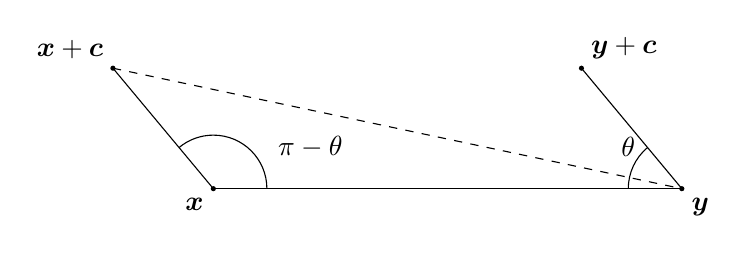
\begin{tikzpicture}[scale=0.85]
  \coordinate (X) at (0,0);
  \coordinate (Y) at (7,0);
  \coordinate (XC) at (-1.5,1.8);
  \coordinate (YC) at (5.5,1.8);
  \draw (X) -- (Y);
  \draw (X) -- (XC);
  \draw (Y) -- (YC);
  \draw[dashed] (XC) -- (Y);
  \fill (X) circle (1.1pt) node[below left] {$\bm{x}$};
  \fill (Y) circle (1.1pt) node[below right] {$\bm{y}$};
  \fill (XC) circle (1.1pt) node[above left] {$\bm{x}+\bm{c}$};
  \fill (YC) circle (1.1pt) node[above right] {$\bm{y}+\bm{c}$};
  \draw (X) ++(0:0.8) arc[start angle=0, end angle=130, radius=0.8];
  \node at (1.45,0.62) {$\pi-\theta$};
  \draw (Y) ++(130:0.8) arc[start angle=130, end angle=180, radius=0.8];
  \node at (6.2,0.62) {$\theta$};
\end{tikzpicture}
\end{center}

若 $\cos\theta\ge 0$，则
\begin{align*}
\abs{(\bm{x}+\bm{c})-\bm{y}}&=\sqrt{a^{2}+\abs{\bm{c}}^{2}+2a\abs{\bm{c}}\cos\theta}\ge\sqrt{a^{2}+\abs{\bm{c}}^{2}}\\
&\ge\sqrt{(\rho-\varepsilon)^{2}+\abs{\bm{c}}^{2}}=\sqrt{\rho^{2}-2\rho\varepsilon+\varepsilon^{2}+\abs{\bm{c}}^{2}}>\sqrt{\rho^{2}+\frac{\abs{\bm{c}}^{2}}{2}}>\rho.
\end{align*}
由此即得 $\operatorname{diam}E<\operatorname{diam}\left(E\cup(E+\bm{c})\right)$．

同理，若 $\cos\theta<0$，则
\[
\abs{(\bm{y}+\bm{c})-\bm{x}}>\rho.
\]
同样得到结论．
\end{solution}

\answerproblem{六、}{20}
设 $a=\sqrt[3]{3}$，$x_{1}=a$，$x_{n+1}=a^{x_{n}}\ (n=1,2,\dots)$．证明：数列 $\{x_{n}\}_{n=1}^{\infty}$ 极限存在，但不是 $3$．

\begin{solution}
易证数列单调上升，有上界 $3$，从而数列极限存在．

具体地，由于 $a=x_{1}=\sqrt[3]{3}>1$，$x_{2}=a^{x_{1}}>a=x_{1}$．一般地，归纳可得 $x_{n+1}=a^{x_{n}}>a^{x_{n-1}}=x_{n}\ (n\ge 2)$．

另一方面，注意到 $a^{3}=3$，归纳可得 $x_{n}\le 3\ (n\ge 1)$．

下证 $\{x_{n}\}$ 的极限不为 $3$．

\textbf{法 I}．我们来归纳地证明 $1<x_{1}<x_{2}<\cdots<x_{n}<\cdots<\frac52$．

具体地，$1<x_{1}=\sqrt[3]{3}=\sqrt[3]{\frac{24}{8}}<\sqrt[3]{\frac{125}{8}}=\frac52$．

假设对某个 $n\ge 1$，$1<x_{n}<\frac52$ 成立，那么
\[
x_{n+1}=a^{x_{n}}<\left(\sqrt[3]{3}\right)^{\frac52}=\sqrt[6]{243},
\]
而另一方面
\[
\left(\frac52\right)^{6}=\left(\frac{25}{4}\right)^{3}=\left(6+\frac14\right)^{3}=216+3\cdot 6^{2}\cdot\frac14+\cdots=243+\cdots>243,
\]
其中 $\cdots$ 显然为正数，故得证 $\sqrt[6]{243}<\frac52$．

由于所有的项 $x_{n}$ 都不超过 $\frac52$，所以数列的极限不可能为 $3$．

\textbf{法 II}．我们来寻找 $\{x_{n}\}$ 的上界 $L$．为此，我们需要关系式 $3^{\frac{L}{3}}\le L$，即 $3^{\frac13}\le L^{\frac1L}$．考虑 $f(x)=x^{\frac1x}\ (x>0)$．我们有
\[
f'(x)=x^{\frac1x}\cdot\frac{1-\ln x}{x^{2}},\qquad x>0.
\]
可见 $f$ 在 $(0,\ee]$ 上严格单增，在 $[\ee,+\infty)$ 上严格单减．我们来归纳地证明 $x_{n}<\ee$．

易见 $x_{1}=3^{\frac13}<\ee^{\frac1e}<\ee$．

若对某个 $n\ge 1$，$x_{n}<\ee$，则 $x_{n+1}=3^{\frac{x_{n}}{3}}<\ee^{\frac{x_{n}}{\ee}}<\ee$．

因此，$\ee$ 是 $\{x_{n}\}$ 的上界．即数列 $\{x_{n}\}$ 的极限不可能为 $3$．

\textbf{法 III}．设 $\{x_{n}\}$ 的极限为 $L$．考察前面关于 $\{x_{n}\}$ 单调有界性的证明，事实上可以得到数列 $\{x_{n}\}$ 严格单增，进而 $x_{n}<L\ (\forall n\ge 1)$．记 $f(x)=a^{x}$，则
\[
f'(3)=a^{3}\ln a=\ln 3>1.
\]

若 $L=3$，由 $f$ 的连续可导性，有 $\delta>0$ 使得当 $x\in(3-\delta,3+\delta)$ 时，$f'(x)>1$．我们有 $N\ge 1$ 使得当 $n\ge N$ 时，$3-\delta<x_{n}<3$．此时，由中值定理，有 $\xi_{n}\in(x_{n},L)$，使得
\[
\abs{x_{n+1}-3}=f(3)-f(x_{n})=f'(\xi_{n})(3-x_{n})\ge 3-x_{n},\qquad n\ge N.
\]
特别，归纳可得
\[
\abs{x_{n}-3}\ge 3-x_{N}>0,\qquad \forall n\ge N.
\]
与 $\{x_{n}\}$ 收敛于 $3$ 矛盾．因此，$\{x_{n}\}$ 的极限不可能是 $3$．
\end{solution}

\answerpaper{数学 B 类}

\answerproblem{一、}{15}
在空间中给定两不同点 $P$ 和 $Q$．过 $P$ 点直线 $L(P)$ 和过 $Q$ 点直线 $L(Q)$ 正交于点 $M$．问：所有可能的正交点 $M$ 构成何种曲面？证明你的结论．
\begin{solution}
在空间中建立直角坐标系，使得线段 $PQ$ 的中点为原点 $O$，直线 $PQ$ 为 $x$ 轴，$P=(-a,0,0)$，$Q=(a,0,0)$（$a>0$）．

设过 $P$ 点直线 $L(P)$ 和过 $Q$ 点直线 $L(Q)$ 正交于 $M=(x,y,z)$ 点，则有
\begin{gather*}
\overrightarrow{PM}\cdot\overrightarrow{QM}=0,\\
(x+a,y,z)\cdot(x-a,y,z)=0,\\
x^{2}+y^{2}+z^{2}=a^{2},
\end{gather*}
为球面．
\end{solution}

\answerproblem{二、}{15}
设 $f(x,y,z)=x^{2}+(y^{2}+z^{2})(1-x)^{3}$．
\begin{enumerate}[label=(\arabic*)]
  \item 计算 $f$ 的驻点．
  \item 求 $f$ 在 $\Sigma$ 上的最小值，其中，$\Sigma$ 是 $\{(x,y,z)\mid |x|\le 2,\ y^{2}+z^{2}\le 4\}$ 的边界．
  \item 求 $f$ 在椭球 $x^{2}+\frac{y^{2}}{2}+\frac{z^{2}}{3}\le 1$ 上的最小值．
\end{enumerate}
\begin{solution}
\textbf{(1)}
\[
\begin{cases}
f_{x}(x,y,z)=2x-3(y^{2}+z^{2})(1-x)^{2},\\
f_{y}(x,y,z)=2y(1-x)^{3},\\
f_{z}(x,y,z)=2z(1-x)^{3}.
\end{cases}
\]
求解 $f_{x}(x_{0},y_{0},z_{0})=f_{y}(x_{0},y_{0},z_{0})=f_{z}(x_{0},y_{0},z_{0})=0$ 的点可得函数在整个空间上只有唯一的驻点 $(x_{0},y_{0},z_{0})=(0,0,0)$．

（注．易见由上述方程的第二式可得 $x_{0}=1$ 或 $y_{0}=0$．但 $x_{0}=1$ 与第一个式子矛盾．因此 $x_{0}=0$，进而又有 $y_{0}=z_{0}=0$．）

\textbf{(2)} $\Sigma=\Sigma_{1}\cup\Sigma_{2}\cup\Sigma_{3}$，其中
\begin{gather*}
\Sigma_{1}=\{(x,y,z)\mid x\in[-2,2],\ y^{2}+z^{2}=4\},\\
\Sigma_{2}=\{(x,y,z)\mid x=2,\ y^{2}+z^{2}\le 4\},\\
\Sigma_{3}=\{(x,y,z)\mid x=-2,\ y^{2}+z^{2}\le 4\}.
\end{gather*}

在 $\Sigma_{1}$ 上，
\[
f(x,y,z)=x^{2}+4(1-x)^{3}=g_{1}(x),\qquad x\in[-2,2].
\]
作为一元函数，考虑 $g_{1}$ 在 $[-2,2]$ 内的驻点：
\[
g_{1}'(\xi)=2\xi-12(1-\xi)^{2}=0.
\]
可得：$\xi_{1}=\frac{3}{2}$，$\xi_{2}=\frac{2}{3}$．

我们有
\[
g_{1}(2)=0,\qquad g_{1}(-2)=112,\qquad g_{1}\Bigl(\frac{3}{2}\Bigr)=\frac{7}{4},\qquad g_{1}\Bigl(\frac{2}{3}\Bigr)=\frac{16}{27}.
\]
故 $f$ 在 $\Sigma_{1}$ 上的最小值为 $0$．

（注：以上讨论说明 $g_{1}(2)=0$ 以及 $g_{1}(-2),g_{1}\bigl(\frac{3}{2}\bigr),g_{1}\bigl(\frac{2}{3}\bigr)\ge 0$ 即可．或不求驻点，直接说明 $g_{1}\ge 0$ 且 $g_{1}(2)=0$．）

在 $\Sigma_{2}$ 上，
\[
f(x,y,z)=4-(y^{2}+z^{2})=g_{2}(x,y)\ge 0,\qquad y^{2}+z^{2}\le 4.
\]
在 $\Sigma_{3}$ 上，
\[
f(x,y,z)=4+27(y^{2}+z^{2})=g_{3}(x,y)\ge 0,\qquad y^{2}+z^{2}\le 4.
\]
故 $f$ 在 $\Sigma$ 上的最小值为 $0$．

\textbf{(3)} 注意到椭球 $x^{2}+\frac{y^{2}}{2}+\frac{z^{2}}{3}\le 1$ 完全在 $\Sigma$ 围成的区域 $\Omega$ 内，而且函数 $f$ 在 $\Omega$ 内有唯一驻点 $(0,0,0)$，$f(0,0,0)=0$．因此，$f$ 在 $\overline{\Omega}$ 上的最小值为 $0$．进而 $f$ 在该椭球上的最小值就是 $0$．
\end{solution}

\answerproblem{三、}{20}
设 $V$ 是复数域 $\C$ 上的 $n$ 维线性空间，$\bm{A}$ 是 $V$ 上的一个线性变换．证明：存在 $\alpha\in V$ 使得 $\{\alpha,\bm{A}\alpha,\cdots,\bm{A}^{n-1}\alpha\}$ 成为 $V$ 的一组基当且仅当对于 $\bm{A}$ 的任一特征值 $\lambda$，$\lambda$ 的几何重数为 $1$．
\begin{solution}
必要性．设存在 $\alpha\in V$ 使得 $\{\alpha,\bm{A}\alpha,\cdots,\bm{A}^{n-1}\alpha\}$ 成为 $V$ 的一组基，显然 $\bm{A}$ 在该基下的矩阵为
\[
A=\begin{pmatrix}
0 & & & & *\\
1 & 0 & & & *\\
 & 1 & \ddots & & \vdots\\
 & & \ddots & 0 & *\\
 & & & 1 & *
\end{pmatrix}.
\]
对任意 $c\in\C$，
\[
cI-A=\begin{pmatrix}
c & & & & *\\
-1 & c & & & *\\
 & -1 & \ddots & & \vdots\\
 & & \ddots & c & *\\
 & & & -1 & *
\end{pmatrix},
\]
其左下角的 $n-1$ 阶子式非零，所以 $\rank(cI-A)\ge n-1$，从而齐次线性方程组
\[
(cI-A)X=0
\]
的解空间维数为 $n-\rank(cI-A)\le 1$．

又对 $\bm{A}$ 的任一特征值 $\lambda$，
\[
(\lambda I-A)X=0
\]
一定有非零解，它的解空间维数 $\ge 1$．所以齐次线性方程组
\[
(\lambda I-A)X=0
\]
的解空间维数为 $1$，即 $\lambda$ 的几何重数为 $1$．

充分性：设 $\bm{A}$ 的互不相同的特征值为 $\lambda_{1},\lambda_{2},\cdots,\lambda_{s}$，代数重数分别为 $d_{1},d_{2},\cdots,d_{s}$，其中 $d_{1}+d_{2}+\cdots+d_{s}=n$，即 $\bm{A}$ 的特征多项式为
\[
f(x)=(x-\lambda_{1})^{d_{1}}(x-\lambda_{2})^{d_{2}}\cdots(x-\lambda_{s})^{d_{s}}.
\]
对于 $1\le i\le s$，记 $V_{\lambda_{i}}=\operatorname{Ker}(\bm{A}-\lambda_{i}\bm{I})^{d_{i}}$，其中 $\bm{I}$ 为恒等变换，则 $V_{\lambda_{i}}$ 为 $\bm{A}$-不变子空间且
\[
V=V_{\lambda_{1}}\oplus V_{\lambda_{2}}\oplus\cdots\oplus V_{\lambda_{s}}.
\]
由于 $\lambda_{i}$ 的几何重数为 $1$，故 $\bm{A}|_{V_{\lambda_{i}}}$ 的 Jordan 标准型为
\[
\begin{pmatrix}
\lambda_{i} & & & \\
1 & \lambda_{i} & & \\
 & \ddots & \ddots & \\
 & & 1 & \lambda_{i}
\end{pmatrix}_{d_{i}\times d_{i}}.
\]
所以存在 $\alpha_{i}\in V_{\lambda_{i}}$ 使得 $(\bm{A}-\lambda_{i}\bm{I})^{d_{i}-1}\alpha_{i}\ne 0$．

令
\[
\alpha=\alpha_{1}+\alpha_{2}+\cdots+\alpha_{s},
\]
则 $\{\alpha,\bm{A}\alpha,\cdots,\bm{A}^{n-1}\alpha\}$ 是 $V$ 的一组基．若否，则 $\alpha,\bm{A}\alpha,\cdots,\bm{A}^{n-1}\alpha$ 线性相关，从而存在次数 $\le n-1$ 的非零多项式 $p(x)\in\C[x]$ 使得 $p(\bm{A})\alpha=0$．由于 $V_{\lambda_{i}}$ 为 $\bm{A}$-不变子空间，所以 $p(\bm{A})\alpha_{i}\in V_{\lambda_{i}}$．由
\[
0=p(\bm{A})\alpha=p(\bm{A})\alpha_{1}+p(\bm{A})\alpha_{2}+\cdots+p(\bm{A})\alpha_{s}
\]
可知 $p(\bm{A})\alpha_{i}=0$．由于 $(\bm{A}-\lambda_{i}\bm{I})^{d_{i}-1}\alpha_{i}\ne 0$，所以 $(x-\lambda_{i})^{d_{i}}$ 是 $\bm{A}$ 的零化 $\alpha_{i}$ 的次数最低的多项式，从而
\[
(x-\lambda_{i})^{d_{i}}\mid p(x).
\]
又当 $i\ne j$ 时，$(x-\lambda_{i})^{d_{i}}$ 与 $(x-\lambda_{j})^{d_{j}}$ 互素，所以
\[
(x-\lambda_{1})^{d_{1}}(x-\lambda_{2})^{d_{2}}\cdots(x-\lambda_{s})^{d_{s}}\mid p(x),
\]
即 $f(x)\mid p(x)$，这与 $\deg p(x)<\deg f(x)$ 且 $p(x)\ne 0$ 矛盾．
\end{solution}

\answerproblem{四、}{15}
证明对任意 $n$ 阶方阵 $A$，存在主对角线上元素为 $1$ 或 $-1$ 的 $n$ 阶对角矩阵 $J$ 使得 $A+J$ 可逆．
\begin{solution}
对 $n$ 做归纳．当 $n=1$ 时，$A=(a)$，显然 $a+1$ 或者 $a-1$ 中一定有一个数非零，结论成立．

设结论对 $n-1$ 阶矩阵成立，下面考察 $n$ 阶方阵 $A$．记
\[
A=\begin{pmatrix}A_{1} & \beta\\ \alpha & a_{nn}\end{pmatrix},
\]
其中 $A_{1}$ 为 $n-1$ 阶矩阵，$\alpha$ 为 $n-1$ 维行向量，$\beta$ 为 $n-1$ 维列向量，$a_{nn}$ 为一个数．由归纳假设，存在主对角线上元素为 $1$ 或 $-1$ 的 $n-1$ 阶对角矩阵 $J_{1}$ 使得 $A_{1}+J_{1}$ 可逆．

从而
\begin{align*}
&\begin{vmatrix}A+\begin{pmatrix}J_{1} & 0\\ 0 & 1\end{pmatrix}\end{vmatrix}
-\begin{vmatrix}A+\begin{pmatrix}J_{1} & 0\\ 0 & -1\end{pmatrix}\end{vmatrix}\\
={}&\begin{vmatrix}A_{1}+J_{1} & \beta\\ \alpha & a_{nn}+1\end{vmatrix}
-\begin{vmatrix}A_{1}+J_{1} & \beta\\ \alpha & a_{nn}-1\end{vmatrix}\\
={}&\begin{vmatrix}A_{1}+J_{1} & \beta-\beta\\ \alpha & (a_{nn}+1)-(a_{nn}-1)\end{vmatrix}\\
={}&2\abs{A_{1}+J_{1}}\ne 0.
\end{align*}
这表明上式最左边的两个行列式中至少有一个非零．

令
\[
J=\begin{pmatrix}J_{1} & 0\\ 0 & 1\end{pmatrix}\quad\text{若}\quad
\begin{vmatrix}A+\begin{pmatrix}J_{1} & 0\\ 0 & 1\end{pmatrix}\end{vmatrix}\ne 0,
\]
或者
\[
J=\begin{pmatrix}J_{1} & 0\\ 0 & -1\end{pmatrix}\quad\text{若}\quad
\begin{vmatrix}A+\begin{pmatrix}J_{1} & 0\\ 0 & -1\end{pmatrix}\end{vmatrix}\ne 0,
\]
则 $J$ 为主对角线上元素为 $1$ 或 $-1$ 的 $n$ 阶对角矩阵且 $\abs{A+J}\ne 0$，即 $A+J$ 可逆，所以结论对 $n$ 阶矩阵成立．

由归纳法原理，结论对任意方阵成立．
\end{solution}

\answerproblem{五、}{15}
设 $f(x)=x^{n}(1-x)^{n}$，
\[
F(x)=f(x)-f''(x)+f^{(4)}(x)-\cdots+(-1)^{n}f^{(2n)}(x).
\]
计算并化简 $\dfrac{\mathrm{d}}{\mathrm{d}x}\bigl(F'(x)\sin x-F(x)\cos x\bigr)$．
\begin{solution}
\begin{align*}
\frac{\dd}{\dd x}\bigl(F'(x)\sin x-F(x)\cos x\bigr)
&=F''(x)\sin x+F'(x)\cos x-F'(x)\cos x+F(x)\sin x\\
&=\bigl(F''(x)+F(x)\bigr)\sin x\\
&=\bigl(f(x)+(-1)^{n}f^{(2n+2)}(x)\bigr)\sin x\\
&=f(x)\sin x=x^{n}(1-x)^{n}\sin x.
\end{align*}
\end{solution}

\answerproblem{六、}{20}
设非负函数 $f$ 在 $[0,+\infty)$ 上连续可微，无穷积分 $\displaystyle\int_{0}^{+\infty}f(x)\dd x$ 收敛，且存在 $[0,+\infty)$ 上的非负函数 $g$，使得
\[
f'(x)\le g(x),\qquad x\ge 0. \tag{1}
\]
分别就下列三种情形，证明 $\displaystyle\lim_{x\to+\infty}f(x)=0$．
\begin{enumerate}[label=(\roman*)]
  \item $\displaystyle\int_{0}^{+\infty}g(x)\dd x$ 收敛．
  \item $g(x)=C>0$，其中 $C$ 为常数．
  \item $g(x)=Cf^{p}(x)$，其中 $C>0$，$p>0$ 为常数．
\end{enumerate}
\begin{solution}
\textbf{法 1}．(i) 由条件 (1)，
\[
f(x)\le f(y)+\int_{y}^{x}g(x)\dd x\le f(y)+\int_{y}^{+\infty}g(x)\dd x,\qquad 0\le y<x.
\]
所以 $f$ 在 $[0,+\infty)$ 上有界．于是
\[
\varlimsup_{x\to+\infty}f(x)\le f(y)+\int_{y}^{+\infty}g(x)\dd x,\qquad 0\le y<+\infty
\]
进而由无穷积分 $\int_{0}^{+\infty}g(x)\dd x$ 收敛，得到
\[
\varlimsup_{x\to+\infty}f(x)\le\varliminf_{x\to+\infty}f(x)
\]
故 $\lim\limits_{x\to+\infty}f(x)=A$ 存在，又无穷积分 $\int_{0}^{+\infty}f(x)\dd x$ 收敛，从而 $A=0$．

(ii) 我们用反证法证明结论．

假设结论不成立，那么存在正数 $a$ 和正数数列 $\{x_{n}\}$，使得 $\lim\limits_{n\to+\infty}x_{n}=+\infty$，$f(x_{n})\ge a$，$n=1,2,\cdots$．显然不妨设
\begin{equation*}
x_{n}>\frac{a}{2C},\qquad n=1,2,\cdots. \tag{2}
\end{equation*}
在区间 $\bigl[x_{n}-\frac{a}{2C},x_{n}\bigr]$ 上对不等式 (1) 从 $x$ 积分到 $x_{n}$，利用 (2) 得到
\[
f(x_{n})-f(x)\le C(x_{n}-x)\ \Rightarrow\ a-f(x)\le C(x_{n}-x)\le C\cdot\frac{a}{2C}=\frac{a}{2}.
\]
我们有
\[
f(x)\ge\frac{a}{2},\qquad x_{n}-\frac{a}{2C}\le x\le x_{n},\ n=1,2,\cdots
\]
从而
\[
\int_{x_{n}-\frac{a}{2C}}^{x_{n}}f(x)\dd x\ge\frac{a}{2}\cdot\frac{a}{2C}=\frac{a^{2}}{4C},\qquad n=0,1,2,\cdots.
\]
此与 $\int_{0}^{+\infty}f(x)\dd x$ 收敛的 Cauchy 准则矛盾，证毕．

(iii) 假设结论不成立，那么存在正数 $a$ 和正数数列 $\{x_{n}\}$，使得 $\lim\limits_{n\to+\infty}x_{n}=+\infty$，$f(x_{n})\ge a$，$n=1,2,\cdots$．显然不妨设
\begin{equation*}
x_{n}>b=\frac{a}{2a^{p-1}C},\qquad n=1,2,\cdots. \tag{3}
\end{equation*}
现在证明 $f$ 在区间 $[x_{n}-b,x_{n}]$ 上的最小值 $m_{n}$ 大于一个正常数．

设 $t_{n}\in[x_{n}-b,x_{n}]$，$f(t_{n})=m_{n}$．我们分两种情况来讨论．

1. $m_{n}=a$，则有 $f(x)\ge a$，$x\in[x_{n}-b,x_{n}]$．

2. $m_{n}<a$，因为 $f(x_{n})\ge a$，所以 $t_{n}<x_{n}$．记 $T_{n}=\sup\{t;f(x)<a,\ x\in[t_{n},t)\}$，那么，由 $f$ 的连续性知道，$t_{n}<T_{n}\le x_{n}$，$f(T_{n})=a$．

在 $t_{n}$ 和 $T_{n}$ 处应用不等式 (1)，利用 (3)，得到
\[
a-m_{n}=f(T_{n})-f(t_{n})\le C\int_{t_{n}}^{T_{n}}f^{p}(x)\dd x\le Ca^{p}(T_{n}-t_{n})\le Ca^{p}b=\frac{a}{2}.
\]
即
\[
\frac{a}{2}\le m_{n}\le f(x),\qquad x\in[x_{n}-b,x_{n}].
\]
综合两种情况，我们总有
\[
f(x)\ge\frac{a}{2},\quad x\in[x_{n}-b,x_{n}].
\]
于是
\[
\int_{x_{n}-b}^{x_{n}}f(x)\dd x\ge\frac{ab}{2}=\frac{a}{4C}>0,
\]
此与 $\int_{0}^{+\infty}f(x)\dd x$ 收敛的 Cauchy 准则矛盾，证毕．

\textbf{法 2}．我们对三种情形作统一处理．设 $g(x)=Cf^{p}(x)+h(x)$，其中 $C\ge 0$，$p\ge 0$ 为常数（$0^{0}$ 理解为 $1$），$h$ 非负且 $\int_{0}^{+\infty}h(x)\dd x$ 收敛．

任取 $m\ge 16C+2$，由 Cauchy 准则，存在 $N=N_{m}\ge 1$ 使得当 $n\ge N$ 时，
\[
\int_{\frac{n}{m^{2}}}^{\frac{n+1}{m^{2}}}\bigl(f(x)+h(x)\bigr)\dd x<\frac{1}{4m^{3}}.
\]
因此，结合 $f$ 非负，对于任何 $n\ge N$，有 $\xi_{n}\in\bigl[\frac{n}{m^{2}},\frac{n+1}{m^{2}}\bigr]$ 使得 $f(\xi_{n})<\frac{1}{4m}$．

我们断言当 $x>\frac{N+1}{m^{2}}$ 时，$f(x)\le\frac{1}{m}$．

否则，有 $\eta_{1}>\frac{N+1}{m^{2}}$，使得 $f(\eta_{1})>\frac{1}{m}$．我们有 $k\ge N$ 使得 $\xi_{k}<\eta_{1}<\xi_{k}+\frac{2}{m^{2}}$．

进一步，设 $\eta_{2}$ 为 $f-\frac{1}{m}$ 在 $[\xi_{k},\eta_{1}]$ 中最小的零点，$\eta_{3}$ 为 $f-\frac{1}{2m}$ 在 $[\xi_{k},\eta_{2}]$ 中最大的零点．则在 $[\eta_{3},\eta_{2}]$ 上 $\frac{1}{2m}\le f\le\frac{1}{m}<1$．从而
\begin{align*}
\frac{1}{2m}&=f(\eta_{2})-f(\eta_{3})=\int_{\eta_{3}}^{\eta_{2}}f'(t)\dd t\\
&\le\int_{\eta_{3}}^{\eta_{2}}\bigl(Cf^{p}(t)+h(t)\bigr)\dd t\le\int_{\eta_{3}}^{\eta_{2}}\bigl(C+h(t)\bigr)\dd t\\
&\le\frac{2C}{m^{2}}+\frac{1}{2m^{3}}\le\frac{1}{4m}.
\end{align*}
矛盾．

因此，当 $x>\frac{N+1}{m}$ 时，$f(x)\le\frac{1}{m}$．由此即得 $\lim\limits_{x\to+\infty}f(x)=0$．
\end{solution}

\answerpaper{非数学 A 类}

\answerproblem{一、}{30}
填空题：
\begin{enumerate}[label=(\arabic*)]
  \item $\displaystyle \lim_{x\to 3}\frac{\sqrt{x^3+9}-6}{2-\sqrt{x^3-23}}=\underline{\hspace{3.5em}}$．
  \item 设 $z=f(x^2-y^2,xy)$，且 $f(u,v)$ 有连续的二阶偏导数，则 $\displaystyle \frac{\partial^2 z}{\partial x\partial y}=\underline{\hspace{3.5em}}$．
  \item 设 $f(x)=\dfrac{1}{x^2-3x+2}$，则 $f^{(n)}(0)=\underline{\hspace{3.5em}}$．
  \item 幂级数 $\displaystyle \sum_{n=1}^{\infty}\frac{(-1)^{n-1}x^{2n}}{n(2n-1)}$ 的收敛域为 $\underline{\hspace{3.5em}}$．
  \item 设曲面 $\Sigma$ 是平面 $y+z=5$ 被柱面 $x^2+y^2=25$ 所截得的部分，则
  \[
    \iint_{\Sigma}(x+y+z)\dd S=\underline{\hspace{6em}}.
  \]
\end{enumerate}
\begin{solution}
\textbf{(1)} 使用洛必达法则，得
\[
\lim_{x\to3}\frac{\sqrt{x^3+9}-6}{2-\sqrt{x^3-23}}
=\lim_{x\to3}\frac{\dfrac{3x^2}{2\sqrt{x^3+9}}}{-\dfrac{3x^2}{2\sqrt{x^3-23}}}
=-\lim_{x\to3}\frac{\sqrt{x^3-23}}{\sqrt{x^3+9}}
=-\frac{1}{3}.
\]

\textbf{(2)}
\begin{align*}
z_x&=2xf_1+yf_2,\\
z_{xy}&=2x\bigl(f_{11}(-2y)+f_{12}x\bigr)+f_2+y\bigl(f_{21}(-2y)+f_{22}x\bigr)\\
&=f_2-4xyf_{11}+2(x^2-y^2)f_{12}+xyf_{22}.
\end{align*}

\textbf{(3)}
\begin{align*}
f(x)&=-\frac{1}{x-1}+\frac{1}{x-2},\\
f^{(n)}(x)&=(-1)^{n+1}n!\left(\frac{1}{(x-1)^{n+1}}-\frac{1}{(x-2)^{n+1}}\right),\\
f^{(n)}(0)&=n!\left(1-\frac{1}{2^{n+1}}\right).
\end{align*}

\textbf{(4)} 因为 $\displaystyle \lim_{n\to\infty}\sqrt[n]{\frac{1}{n(2n-1)}}=1$，所以收敛半径为 $1$．

当 $x=\pm1$ 时，$\displaystyle \sum_{n=1}^{\infty}\frac{(-1)^{n-1}}{n(2n-1)}$ 绝对收敛，故收敛域为 $[-1,1]$．

\textbf{(5)} $\Sigma$ 的方程为 $z=5-y$，故
\[
\dd S=\sqrt{2}\dd x\dd y.
\]
$\Sigma$ 在 $xOy$ 平面的投影 $D_{xy}:x^2+y^2\le25$，故
\[
I=\sqrt{2}\iint_{D_{xy}}(x+5)\dd x\dd y
=5\sqrt{2}\iint_{D_{xy}}\dd x\dd y
=125\sqrt{2}\pi.
\]
\end{solution}

\answerproblem{二、}{14}
解方程
\[
(x^2+y^2+3)\frac{\dd y}{\dd x}=2x\left(2y-\frac{x^2}{y}\right).
\]
\begin{solution}
原方程变形为
\[
\frac{y\dd y}{x\dd x}=\frac{2(2y^2-x^2)}{x^2+y^2+3}.
\]
令 $u=x^2$，$v=y^2$，则原方程化为
\[
\frac{\dd v}{\dd u}=\frac{2(2v-u)}{u+v+3}.
\]
解方程 $2v-u=0$，$u+v+3=0$，得到 $u=-2$，$v=-1$，再令 $U=u+2$，$V=v+1$，上述方程化为
\[
\frac{\dd V}{\dd U}=\frac{2(2V-U)}{U+V}.
\]
作变量替换 $W=\frac{V}{U}$ 得到
\[
U\frac{\dd W}{\dd U}=-\frac{W^2-3W+2}{W+1}.
\]
这是分离变量方程，解之得
\[
U(W-2)^3=C(W-1)^2,
\]
回代得
\[
(y^2-2x^2-3)^3=C(y^2-x^2-1)^2.
\]
\end{solution}

\answerproblem{三、}{14}
设 $\Sigma_1$ 是以 $(0,4,0)$ 为顶点且与曲面
\[
\Sigma_2:\ \frac{x^2}{3}+\frac{y^2}{4}+\frac{z^2}{3}=1\quad(y>0)
\]
相切的圆锥面，求曲面 $\Sigma_1$ 与 $\Sigma_2$ 所围成的空间区域的体积．
\begin{solution}
设 $L$ 是 $xOy$ 平面上过点 $(0,4)$ 且与 $\frac{x^2}{3}+\frac{y^2}{4}=1$ 相切于点 $(x_0,y_0)$ 的直线，则
\[
\frac{x_0^2}{3}+\frac{y_0^2}{4}=1
\quad\text{且切线斜率}\quad
\frac{y_0-4}{x_0}=-\frac{4x_0}{3y_0},
\]
解得 $x_0=\pm\frac{3}{2}$，$y_0=1$．

显然，$\Sigma_1$ 与 $\Sigma_2$ 分别是切线 $L$ 和曲线 $\frac{x^2}{3}+\frac{y^2}{4}=1$ 绕 $y$ 轴旋转而成的曲面，它们的交线位于平面 $y=1$ 上．

记该平面与 $\Sigma_1$、$\Sigma_2$ 围成的空间区域分别记为 $\Omega_1$ 和 $\Omega_2$．

由于 $\Sigma_1$ 是底面圆的半径为 $\frac{3}{2}$，高为 $3$ 的圆锥体，所以其体积
\[
V_1=\frac{1}{3}\pi\left(\frac{3}{2}\right)^2\cdot3=\frac{9\pi}{4}.
\]
又 $\Omega_2$ 的体积为
\[
V_2=\iiint_{\Omega_2}\dd V
=\int_1^2\dd y\iint_{x^2+z^2\le3\left(1-\frac{y^2}{4}\right)}\dd x\dd z
=\pi\int_1^2 3\left(1-\frac{y^2}{4}\right)\dd y
=\frac{5\pi}{4}.
\]
因此，曲面 $\Sigma_1$ 与 $\Sigma_2$ 所围成的空间区域的体积为
\[
\frac{9\pi}{4}-\frac{5\pi}{4}=\pi.
\]
\end{solution}

\answerproblem{四、}{14}
设
\[
I_n=n\int_1^a\frac{\dd x}{1+x^n},
\]
其中 $a>1$．求极限 $\displaystyle \lim_{n\to\infty}I_n$．
\begin{solution}
记 $b=\frac{1}{a}$，则 $0<b<1$．作变量替换 $x=\frac{1}{t}$，得到
\[
I_n=\int_b^1\frac{nt^{n-1}}{t(1+t^n)}\dd t
=\int_b^1\frac{\dd\left(\ln(1+t^n)\right)}{t}.
\]
分部积分得
\[
I_n=\ln2-\frac{\ln(1+b^n)}{b}+\int_b^1\frac{\ln(1+t^n)}{t^2}\dd t.
\]
当 $t\in[b,1]$ 时，$\displaystyle \frac{\ln(1+t^n)}{t^2}\le t^{n-2}$，
\[
0\le\int_b^1\frac{\ln(1+t^n)}{t^2}\dd t
\le\int_b^1 t^{n-2}\dd t
=\frac{1-b^{n-1}}{n-1}.
\]
显然，$\displaystyle \lim_{n\to\infty}\frac{1-b^{n-1}}{n-1}=0$．由夹逼准则，$\displaystyle \lim_{n\to\infty}\int_b^1\frac{\ln(1+t^n)}{t^2}\dd t=0$．

又 $\displaystyle \lim_{n\to\infty}\frac{\ln(1+b^n)}{b}=0$，$\displaystyle \lim_{n\to\infty}I_n=\ln2$．
\end{solution}

\answerproblem{五、}{14}
设 $f(x)$ 在 $[0,1]$ 上有连续的导数且 $f(0)=0$．求证：
\[
\int_0^1 f^2(x)\dd x\le4\int_0^1(1-x)^2|f'(x)|^2\dd x,
\]
并求使上式成为等式的 $f(x)$．
\begin{solution}
由分部积分法
\begin{align*}
\int_0^1 f^2(x)\dd x
&=\left.(x-1)f^2(x)\right|_0^1-\int_0^1(x-1)2f(x)f'(x)\dd x\\
&=2\int_0^1(1-x)f'(x)\cdot f(x)\dd x.
\end{align*}
由 Cauchy 积分不等式，有
\[
\int_0^1(1-x)f'(x)\cdot f(x)\dd x
\le\left(\int_0^1(1-x)^2(f'(x))^2\dd x\right)^{\frac{1}{2}}
\left(\int_0^1 f^2(x)\dd x\right)^{\frac{1}{2}}.
\]
于是
\[
\int_0^1 f^2(x)\dd x\le4\int_0^1(1-x)^2|f'(x)|^2\dd x.
\]
等式成立时应有常数 $c$ 使得 $(1-x)f'(x)=cf(x)$．因此当 $x\in(0,1)$ 时，有
\[
\left((1-x)^cf(x)\right)'
=(1-x)^{c-1}\left((1-x)f'(x)-cf(x)\right)=0.
\]
因而存在常数 $d$ 使得 $f(x)=d(1-x)^{-c}$（$0<x<1$）．
当 $x\to0$ 时，$f(x)\to0$，故 $d=0$．于是 $f\equiv0$．所以使得题中不等式成为等式的函数是 $f(x)=0$．
\end{solution}

\answerproblem{六、}{14}
设数列 $\{x_n\}$ 满足
\[
x_0=\frac{1}{3},\qquad x_{n+1}=\frac{x_n^2}{1-x_n+x_n^2},\quad n\ge0.
\]
证明：无穷级数 $\displaystyle \sum_{n=0}^{\infty}x_n$ 收敛并求其和．
\begin{solution}
\textbf{方法 1.} 根据数学归纳法可知 $x_n>0$．

此外，
\[
x_{n+1}-x_n=-\frac{x_n(1-x_n)^2}{1-x_n+x_n^2}<0.
\]
故 $x_n$ 单调递减，$x_n\le\frac{1}{3}$．

于是，
\[
x_{n+1}=x_n\cdot\frac{x_n}{1-x_n+x_n^2}\le\frac{4}{9}x_n,
\]
$x_n$ 收敛于 $0$．

令 $f(x)=\frac{x}{1+x}$，$x>0$，不难验证 $f(x)$ 严格单调递增且其反函数为 $f^{-1}(x)=\frac{x}{1-x}$．
注意到 $x_{n+1}=f\left(f^{-1}(x_n)-x_n\right)$，故
\[
f^{-1}(x_{n+1})=f^{-1}(x_n)-x_n,\qquad
x_n=f^{-1}(x_n)-f^{-1}(x_{n+1}).
\]
\[
\sum_{i=0}^n x_i=f^{-1}(x_0)-f^{-1}(x_{n+1}).
\]
\[
\sum_{i=0}^{\infty}x_i=f^{-1}(x_0)-f^{-1}(0)=\frac{1}{2}.
\]

\textbf{方法 2.} 证明 $x_n$ 收敛于 $0$ 同方法 1．

注意到
\[
x_n=\frac{x_n}{1-x_n}-\frac{x_{n+1}}{1-x_{n+1}}.
\]
\[
\sum_{i=0}^n x_i=\frac{x_0}{1-x_0}-\frac{x_{n+1}}{1-x_{n+1}}.
\]
\[
\sum_{i=0}^{\infty}x_i=\frac{x_0}{1-x_0}=\frac{1}{2}.
\]
\end{solution}

\answerpaper{非数学 B 类}

\answerproblem{一、}{30}
填空题：
\begin{enumerate}[label=(\arabic*)]
  \item $\lim\limits_{x\to\infty}\left(\dfrac{x+3}{x+2}\right)^{2x-1}=$ \underline{\hspace{6em}}。
  \item 设 $z=f(x^2-y^2,xy)$，且 $f(u,v)$ 有连续的二阶偏导数，则 $\dfrac{\partial^2 z}{\partial x\partial y}=$ \underline{\hspace{6em}}。
  \item 设曲线 $y=\ln(1+ax)+1$ 与曲线 $y=2xy^3+b$ 在 $(0,1)$ 处相切，则 $a+b=$ \underline{\hspace{6em}}。
  \item 设函数 $y=y(x)$ 由方程 $y=1+\arctan(xy)$ 所确定，则 $y'(0)=$ \underline{\hspace{6em}}。
  \item 计算 $\displaystyle\int_0^1 \dd x\int_x^{\sqrt{x}}\frac{\cos y}{y}\dd y=$ \underline{\hspace{6em}}。
\end{enumerate}
\begin{solution}
\textbf{(1)} $\lim\limits_{x\to\infty}\left(1+\dfrac{1}{x+2}\right)^{2(x+2)-5}=\ee^2$。

\textbf{(2)}
\begin{align*}
z_x &= 2x f_1 + y f_2,\\
z_{xy} &= 2x\left(f_{11}(-2y) + x f_{12}\right) + f_2 + y\left(f_{21}(-2y) + x f_{22}\right)\\
&= f_2 - 4xy f_{11} + 2(x^2 - y^2) f_{12} + xy f_{22}.
\end{align*}

\textbf{(3)} 易得 $b=1$，$a=2$，故 $a+b=3$。

\textbf{(4)} 易得 $y'(x)=\dfrac{xy'+y}{1+x^2y^2}$。当 $x=0$ 时，$y'(0)=1$。

\textbf{(5)} 交换积分顺序，得
\[ \int_0^1 \dd x\int_x^{\sqrt{x}}\frac{\cos y}{y}\dd y=\int_0^1 \dd y\int_{y^2}^{y}\frac{\cos y}{y}\dd x=\int_0^1(1-y)\cos y\dd y=1-\cos 1. \]
\end{solution}

\answerproblem{二、}{14}
设曲线 $y=3ax^2+2bx+\ln c$ 经过 $(0,0)$ 点，且当 $0\le x\le 1$ 时 $y\ge 0$。设该曲线与直线 $x=1$，$x$ 轴所围图形的平面图形 $D$ 的面积为 $1$。试求常数 $a,b,c$ 的值，使得 $D$ 绕 $x$ 轴一周后，所得旋转体的体积最小。

\begin{solution}
由于曲线 $y=3ax^2+2bx+\ln c$ 经过 $(0,0)$ 点，故 $\ln c=0$，$c=1$。$D$ 的面积
\[ A=\int_0^1(3ax^2+2bx)\dd x=a+b=1. \]
$D$ 绕 $x$ 轴一周所得到的旋转体体积
\begin{align*}
V &= \pi\int_0^1(3ax^2+2bx)^2\dd x\\
&= \pi\left(\frac{9}{5}a^2+3ab+\frac{4}{3}b^2\right)\\
&= \pi\left(\frac{2}{15}a^2+\frac{1}{3}a+\frac{4}{3}\right).
\end{align*}
\[ V'(a)=\pi\left(\frac{4}{15}a+\frac{1}{3}\right). \]
不难得到，当 $a=-\dfrac{5}{4}$ 时，旋转体得体积最小，此时，$b=\dfrac{9}{4}$，$c=1$。

注：推导最小值点时，用其他办法如配方也可以。
\end{solution}

\answerproblem{三、}{14}
解方程
\[ (x^2+y^2+3)\frac{\dd y}{\dd x}=2x\left(2y-\frac{x^2}{y}\right). \]

\begin{solution}
原方程变形为
\[ \frac{y\dd y}{x\dd x}=\frac{2(2y^2-x^2)}{x^2+y^2+3}. \]
令 $u=x^2$，$v=y^2$，则原方程化为
\[ \frac{\dd v}{\dd u}=\frac{2(2v-u)}{u+v+3}. \]
解方程 $2v-u=0$，$u+v+3=0$，得到 $u=-2$，$v=-1$，再令 $U=u+2$，$V=v+1$，上述方程化为
\[ \frac{\dd V}{\dd U}=\frac{2(2V-U)}{U+V}. \]
作变量替换 $W=\dfrac{V}{U}$ 得到
\[ U\frac{\dd W}{\dd U}=-\frac{W^2-3W+2}{W+1}. \]
这是分离变量方程，解之得 $U(W-2)^3=C(W-1)^2$，回代得
\[ (y^2-2x^2-3)^3=C(y^2-x^2-1)^2. \]
\end{solution}

\answerproblem{四、}{14}
求幂级数 $\displaystyle\sum_{n=1}^{\infty}\frac{(-1)^{n-1}x^{2n}}{n(2n-1)}$ 的收敛域及和函数。

\begin{solution}
因为 $\lim\limits_{n\to\infty}\sqrt[n]{\dfrac{1}{n(2n-1)}}=1$，所以收敛半径为 $1$。

当 $x=\pm1$ 时，$\displaystyle\sum_{n=1}^{\infty}\frac{(-1)^{n-1}}{n(2n-1)}$ 绝对收敛，故收敛域为 $[-1,1]$。

记该幂级数的和函数为 $S(x)$，则在 $(-1,1)$ 上，
\[ \frac{1}{2}S''(x)=\sum_{n=1}^{\infty}(-1)^{n-1}x^{2n-2}=\frac{1}{1+x^2}. \]
\[ S'(x)=2\int_0^x\frac{1}{1+s^2}\dd s=2\arctan x,\quad x\in(-1,1). \]
\[ S(x)=2\int_0^x\arctan s\dd s=2x\arctan x-\ln(1+x^2),\quad x\in(-1,1). \]
由于 $S(x)$ 在收敛域上连续，所以
\[ S(x)=2\int_0^x\arctan s\dd s=2x\arctan x-\ln(1+x^2),\quad x\in[-1,1]. \]
\end{solution}

\answerproblem{五、}{14}
设 $f(x)$ 在 $[0,1]$ 上可导且 $f(0)>0$，$f(1)>0$，$\displaystyle\int_0^1 f(x)\dd x=0$。证明：
\begin{enumerate}[label=(\arabic*)]
  \item $f(x)$ 在 $[0,1]$ 上至少有两个零点；
  \item 在 $(0,1)$ 内至少存在一点 $\xi$，使得 $f'(\xi)+3f^3(\xi)=0$。
\end{enumerate}

\begin{solution}
\textbf{证明. (1)} 首先我在 $(0,1)$ 上至少存在一点 $x_0$ 使得 $f(x_0)<0$。否则若对于任意的 $x\in[0,1]$，$f(x)\ge 0$。$f(x)$ 连续且不恒为零，故 $\int_0^1 f(x)\dd x>0$。与题设矛盾。

其次，因为 $f(x)$ 连续，在区间 $[0,x_0]$ 和 $[x_0,1]$ 上分别应用零点定理知，存在 $\xi_1\in(0,x_0)$，$\xi_2\in(x_0,1)$ 使得 $f(\xi_1)=0$，$f(\xi_2)=0$。

\textbf{(2)} 令 $F(x)=f(x)\ee^{\int_0^x 3f^2(s)\dd s}$，则 $F$ 在 $[0,1]$ 上连续，$(0,1)$ 上可导且 $F(\xi_1)=F(\xi_2)=0$。由罗尔定理，存在 $\xi\in(\xi_1,\xi_2)\subset(0,1)$ 使得 $F'(\xi)=0$。

又 $F'(x)=\left(f'(x)+3f^3(x)\right)\ee^{\int_0^x 3f^2(s)\dd s}$，所以 $f'(\xi)+3f^3(\xi)=0$。
\end{solution}

\answerproblem{六、}{14}
设 $f(x)$ 在 $[0,1]$ 上有连续的导数且 $f(0)=0$。求证：
\[ \int_0^1 f^2(x)\dd x\le 4\int_0^1(1-x)^2|f'(x)|^2\dd x, \]
并求使上式成为等式的 $f(x)$。

\begin{solution}
由分部积分法
\begin{align*}
\int_0^1 f^2(x)\dd x &= (x-1)f^2(x)\Big|_0^1-\int_0^1(x-1)2f(x)f'(x)\dd x\\
&= 2\int_0^1(1-x)f'(x)\cdot f(x)\dd x.
\end{align*}
由 Cauchy 积分不等式，有
\[ \int_0^1(1-x)f'(x)\cdot f(x)\dd x\le\left(\int_0^1(1-x)^2(f'(x))^2\dd x\right)^{\frac{1}{2}}\left(\int_0^1 f^2(x)\dd x\right)^{\frac{1}{2}}. \]
于是
\[ \int_0^1 f^2(x)\dd x\le 4\int_0^1(1-x)^2|f'(x)|^2\dd x. \]
等式成立时应有常数 $c$ 使得 $(1-x)f'(x)=cf(x)$。因此当 $x\in(0,1)$ 时，有
\[ \left((1-x)^cf(x)\right)'=(1-x)^{c-1}\left((1-x)f'(x)-cf(x)\right)=0. \]
因而存在常数 $d$ 使得 $f(x)=d(1-x)^{-c}$（$0<x<1$）。

当 $x\to0$ 时，$f(x)\to0$，故 $d=0$。于是 $f=0$。所以使得题中不等式成为等式的函数是 $f(x)=0$。
\end{solution}

\yearchapter{2024}{第十六届}
\answerpaper{数学 A 类}

\answerproblem{一、}{15}
设双叶双曲面 $S: x^2+y^2-z^2=-2$．记以 $M_0(1,1,-1)$ 为顶点且与 $S$ 的上半叶
\[
  S^+ = \{(x,y,z)\in S \mid z\ge\sqrt{2}\}
\]
相切的所有切线构成的锥面为 $\Sigma$．
\begin{enumerate}[label=(\arabic*)]
  \item 求锥面 $\Sigma$ 的方程；
  \item 求 $S^+\cap\Sigma$ 所在平面 $\pi$ 的方程．
\end{enumerate}

\begin{solution}
\textbf{(1)} 设过顶点 $M(1,1,-1)$，方向向量为 $(l,m,n)$ 的直线的参数方程为
\begin{equation}
  L:\begin{cases}
    x-1=lt,\\
    y-1=mt,\\
    z+1=nt.
  \end{cases}\tag{1}
\end{equation}
将 (1) 代入 $S$ 的方程可得
\[
  (1+lt)^2+(1+mt)^2-(-1+nt)^2+2=0.
\]
即
\begin{equation}
  (l^2+m^2-n^2)t^2+2(l+m+n)t+3=0.\tag{2}
\end{equation}
既然 $L$ 与 $S$ 相切，由 (2) 则有
\[
  4(l+m+n)^2-12(l^2+m^2-n^2)=0.
\]
即
\begin{equation}
  l^2+m^2-2n^2-lm-ln-mn=0.\tag{3}
\end{equation}
结合 (1) 与 (3)，消去参数 $t$ 可得锥面方程
\[
  (x-1)^2+(y-1)^2-2(z+1)^2-(x-1)(y-1)-(x-1)(z+1)-(y-1)(z+1)=0.
\]

\textbf{(2)} 对于任意的 $M_1(x_1,y_1,z_1)\in S^+\cap\Sigma$，设 $M(x,y,z)$ 是连接 $M_0$ 与 $M_1$ 的直线上任意一点，并设 $\overrightarrow{M_1M}=t\overrightarrow{M_0M_1}$，其中 $t$ 为参数．于是有
\begin{equation}
  \begin{cases}
    x-x_1=t(x_1-1),\\
    y-y_1=t(y_1-1),\\
    z-z_1=t(z_1+1).
  \end{cases}\tag{4}
\end{equation}
将 (4) 与 $S^+$ 的方程联立则有
\begin{equation}
  \bigl(x_1(1+t)-t\bigr)^2+\bigl(y_1(1+t)-t\bigr)^2-\bigl(z_1(1+t)+t\bigr)^2+2=0.\tag{5}
\end{equation}
利用 $x_1^2+y_1^2-z_1^2=-2$，由 (5) 可得
\begin{equation}
  (-1-2x_1-2y_1+2z_1)t^2-2(x_1+y_1+z_1+2)t=0.\tag{6}
\end{equation}
由于 $M_1(x_1,y_1,z_1)$ 是切点，因此有 $x_1+y_1+z_1+2=0$，因此所求的平面 $\pi$ 的方程为
\[
  x+y+z+2=0.
\]
\end{solution}

\answerproblem{二、}{15}
设 $s\ge 0$，
\[
  \varphi(s)=\int_0^{+\infty}\frac{\ln(1+sx^2)}{x(1+x^2)}\dd x.
\]
求 $\varphi(1)$ 和 $\varphi(2)$．

\begin{solution}
我们有 $\lim\limits_{x\to 0^+}\dfrac{\ln(1+x)}{\sqrt{x}}=0$，$\lim\limits_{x\to+\infty}\dfrac{\ln(1+x)}{\sqrt{x}}=0$．因此，有常数 $C>0$，使得
\[
  \ln(1+x)\le C\sqrt{x},\qquad \forall x>0.
\]
从而，
\[
  \frac{\ln(1+sx^2)}{x(1+x^2)}\le C\frac{\sqrt{s}}{1+x^2},\qquad \forall x>0,\ s\ge 0.
\]
因此，广义积分 $\displaystyle\int_0^{+\infty}\frac{\ln(1+sx^2)}{x(1+x^2)}\dd x$ 关于 $s\in[0,+\infty)$ 内闭一致收敛．进而 $\varphi$ 在 $[0,+\infty)$ 上连续．

另一方面，由
\[
  \frac{x}{(1+x^2)(1+sx^2)}\le \frac{1}{2\sqrt{s}(1+x^2)},\qquad \forall x>0,\ s>0
\]
可得，积分 $\displaystyle\int_0^{+\infty}\frac{\ln(1+sx^2)}{x(1+x^2)}\dd x$ 形式求导后得到的积分 $\displaystyle\int_0^{+\infty}\frac{x}{(1+x^2)(1+sx^2)}\dd x$ 关于 $s\in(0,+\infty)$ 内闭一致收敛．因此，$\varphi$ 在 $(0,+\infty)$ 内连续可导且
\begin{align*}
  \varphi'(s)&=\int_0^{+\infty}\frac{x}{(1+x^2)(1+sx^2)}\dd x\\
  &=\frac{1}{1-s}\int_0^{+\infty}\Bigl(\frac{x}{1+x^2}-\frac{sx}{1+sx^2}\Bigr)\dd x\\
  &=\frac{1}{2(1-s)}\ln\frac{1+x^2}{1+sx^2}\biggr|_{x=0}^{+\infty}=-\frac{\ln s}{2(1-s)}.
\end{align*}
（上式当 $s=1$ 时理解为相应的极限，或不妨只考虑 $s\ne 1$ 的情形）

结合 $\varphi(0)=0$，得到
\begin{align*}
  \varphi(1)&=-\int_0^1\frac{\ln s}{2(1-s)}\dd s=-\int_0^1\frac{\ln(1-s)}{2s}\dd s\\
  &=-\lim_{\varepsilon\to 0^+}\int_0^{1-\varepsilon}\frac{\ln(1-s)}{2s}\dd s
   =\lim_{\varepsilon\to 0^+}\int_0^{1-\varepsilon}\sum_{n=1}^{\infty}\frac{s^{n-1}}{2n}\dd s\\
  &=\lim_{\varepsilon\to 0^+}\sum_{n=1}^{\infty}\int_0^{1-\varepsilon}\frac{s^{n-1}}{2n}\dd s
   =\lim_{\varepsilon\to 0^+}\sum_{n=1}^{\infty}\frac{(1-\varepsilon)^n}{2n^2}\\
  &=\sum_{n=1}^{\infty}\frac{1}{2n^2}=\frac{\pi^2}{12}.
\end{align*}

同理，
\begin{align*}
  \varphi(2)&=-\int_0^2\frac{\ln s}{2(1-s)}\dd s=-\int_{-1}^1\frac{\ln(1-s)}{2s}\dd s\\
  &=-\lim_{\varepsilon\to 0^+}\int_{-(1-\varepsilon)}^{1-\varepsilon}\frac{\ln(1-s)}{2s}\dd s
   =\lim_{\varepsilon\to 0^+}\int_{-(1-\varepsilon)}^{1-\varepsilon}\sum_{n=1}^{\infty}\frac{s^{n-1}}{2n}\dd s\\
  &=\lim_{\varepsilon\to 0^+}\sum_{n=1}^{\infty}\int_{-(1-\varepsilon)}^{1-\varepsilon}\frac{s^{n-1}}{2n}\dd s
   =\lim_{\varepsilon\to 0^+}\sum_{n=0}^{\infty}\frac{(1-\varepsilon)^{2n+1}}{(2n+1)^2}\\
  &=\sum_{n=0}^{\infty}\frac{1}{(2n+1)^2}=\frac{\pi^2}{8}.
\end{align*}

\textbf{注.} 计算中有多种其它方法，例如，可利用
\begin{align*}
  \int_0^1\frac{\ln(1+s)}{s}\dd s&=\int_0^1\frac{\ln(1-s^2)-\ln(1-s)}{s}\dd s\\
  &=\int_0^1\frac{\ln(1-s)}{2s}\dd s-\int_0^1\frac{\ln(1-s)}{s}\dd s
   =-\int_0^1\frac{\ln(1-s)}{2s}\dd s;
\end{align*}
\begin{align*}
  \int_0^1\frac{\ln(1-s)}{s}\dd s
  &=\lim_{\beta\to 1^-}\lim_{\alpha\to 0^+}\int_0^1\frac{(1-s)^\alpha\ln(1-s)}{s^\beta}\dd s\\
  &=\lim_{\beta\to 1^-}\lim_{\alpha\to 0^+}\frac{\dd}{\dd\alpha}\int_0^1\frac{(1-s)^\alpha}{s^\beta}\dd s.
\end{align*}
\end{solution}

\answerproblem{三、}{20}
设
\[
  A=\begin{pmatrix}
    a_{11} & a_{12} & a_{13}\\
    a_{21} & a_{22} & a_{23}\\
    a_{31} & a_{32} & a_{33}
  \end{pmatrix}
\]
为实数域 $\R$ 上的 $3\times 3$ 不可逆方阵．若 $A$ 的伴随矩阵 $A^*$ 为
\[
  A^*=\begin{pmatrix}
    a_{11}^2 & a_{12}^2 & a_{13}^2\\
    a_{21}^2 & a_{22}^2 & a_{23}^2\\
    a_{31}^2 & a_{32}^2 & a_{33}^2
  \end{pmatrix},
\]
求 $A$．

\begin{solution}
\textbf{(1)} 由矩阵 $A$ 不可逆知 $\rank(A^*)=0$ 或 $1$．

\textbf{(2)} 若 $\rank(A^*)=0$，则显然有 $A^*=0$，进而 $A=0$．

\textbf{(3)} 若 $\rank(A^*)=1$，则 $A^*$ 的任何 $2$ 阶子式皆为 $0$．特别地有
\[
  \begin{vmatrix}
    a_{11}^2 & a_{12}^2\\
    a_{21}^2 & a_{22}^2
  \end{vmatrix}=0,\qquad
  \begin{vmatrix}
    a_{21}^2 & a_{22}^2\\
    a_{31}^2 & a_{32}^2
  \end{vmatrix}=0,\qquad
  \begin{vmatrix}
    a_{11}^2 & a_{12}^2\\
    a_{31}^2 & a_{32}^2
  \end{vmatrix}=0.
\]
于是得到
\[
  \begin{cases}
    a_{11}a_{22}=\pm a_{12}a_{21},\\
    a_{21}a_{32}=\pm a_{22}a_{31},\\
    a_{12}a_{31}=\pm a_{11}a_{32}.
  \end{cases}
\]
如果上面三个等式中有某个等式的正号成立，不妨设 $a_{11}a_{22}=a_{12}a_{21}$，于是 $A$ 有子式
\[
  \begin{vmatrix}
    a_{11} & a_{12}\\
    a_{21} & a_{22}
  \end{vmatrix}=0,
\]
它是矩阵 $A$ 中元素 $a_{33}$ 的代数余子式，由伴随矩阵 $A^*$ 的定义得到 $a_{33}^2=0$，即 $a_{33}=0$．如果上面三个等式中每个等式出现的都是负号，则将该三个等式的左右两边分别相乘得
\[
  a_{11}a_{22}a_{21}a_{32}a_{12}a_{31}=-a_{11}a_{22}a_{21}a_{32}a_{12}a_{31},
\]
从而 $a_{11},a_{12},a_{21},a_{22},a_{31},a_{32}$ 中至少有一个为 $0$．总之 $A^*$ 至少有一个元素是 $0$．

不妨设 $a_{11}^2=0$．若 $A^*$ 的第一列不全为 $0$，则由 $\rank(A^*)=1$ 知 $A^*$ 的第二列和第三列皆可由 $A^*$ 的第一列线性表出，故 $A^*$ 的第一行元素全部为 $0$．从而 $A^*$ 有一整行元素全为 $0$ 或有一整列元素全为 $0$．相应地，$A$ 也有一整行元素全为 $0$ 或有一整列元素全为 $0$．不妨设 $A$ 的第一行元素全为 $0$，此时 $A$ 的其它元素的代数余子式全为 $0$，故 $a_{22}^2=a_{23}^2=a_{32}^2=a_{33}^2=0$．这表明在矩阵 $A$ 中有 $a_{22}=a_{23}=a_{32}=a_{33}=0$，所以矩阵 $A$ 的元素 $a_{12}$ 和 $a_{13}$ 的代数余子式都是 $0$，由 $A^*$ 的定义得到 $a_{21}^2=a_{31}^2=0$，这导致 $A^*=0$，与 $\rank(A^*)=1$ 矛盾．故我们总有 $A=0$．
\end{solution}

\answerproblem{四、}{15}
熟知实数域 $\R$ 上的一元多项式集合 $\R[x]$ 在多项式加法和数乘下构成 $\R$ 上的一个线性空间．设 $f_i(x)\in\R[x]$ 且次数为 $n_i$，$1\le i\le 2024$，这里规定零多项式的次数为 $-\infty$，已知
\[
  \sum_{i=1}^{2024} n_i<2047276,
\]
证明：$f_1(x),f_2(x),\cdots,f_{2024}(x)$ 为空间 $\R[x]$ 中线性相关的向量组．

\begin{solution}
记向量组 $f_1(x),f_2(x),\cdots,f_{2024}(x)$ 为向量组 (I)，若向量组 (I) 中有零多项式 $0$，即包含 $\R[x]$ 中的零元，则显然向量组 (I) 线性相关．若向量组 (I) 中每个多项式都是非零多项式，则向量组 (I) 中一定有两个次数相同的多项式．事实上，若 $n_1,n_2,\cdots,n_{2024}$ 两两不同，不失一般性可假设 $n_1<n_2<\cdots<n_{2024}$．于是 $n_i\ge i-1$，进而
\[
  \sum_{i=1}^{2024} n_i\ge \sum_{i=1}^{2024}(i-1)=\frac{2023\times 2024}{2}=2047276,
\]
矛盾．

由于向量组 (I) 中存在次数相同的两个多项式，不妨设 $n_i=n_j=n$，$j>i$，且有
\[
  f_i(x)=ax^n+\cdots,\qquad f_j(x)=bx^n+\cdots,
\]
其中 $a,b\ne 0$．令 $g(x)=f_i(x)-\dfrac{a}{b}f_j(x)$，则显然有向量组 (I) 与向量组 (II)：
\[
  f_1(x),\cdots,f_{i-1}(x),g(x),f_{i+1}(x),\cdots,f_j(x),\cdots,f_{2024}(x)
\]
等价．

注意到 $\deg g(x)<\deg f_i(x)$，故向量组 (II) 中多项式的次数之和小于 $\displaystyle\sum_{i=1}^{2024}n_i<2047276$．类似地，向量组 (II) 中一定有零多项式或者有两个次数相同的多项式，从而向量组 (II) 线性相关或者得到与向量组 (II) 等价的向量组 (III) 且向量组 (III) 中多项式次数之和小于向量组 (II) 中多项式的次数之和，又由向量组等价的传递性易知向量组 (III) 与向量组 (I) 等价．重复前述过程，每一步都可以得到一个与之前向量组等价的向量组使得其若不包含零多项式时其中多项式的次数之和更低，这个过程一直进行下去，最后我们可以得到与向量组 (I) 等价的向量组 (IV)，其中的多项式的次数之和 $<0$．由此得到向量组 (IV) 中一定包含零多项式，所以向量组 (IV) 在 $\R[x]$ 中线性相关．由等价性，向量组 (I)，即 $f_1(x),f_2(x)\cdots,f_{2024}(x)$，在 $\R[x]$ 中线性相关．
\end{solution}

\answerproblem{五、}{15}
讨论以下级数的收敛性：
\[
  \sum_{n=2}^{\infty}\frac{(-1)^n}{n+(-1)^{[\sqrt{n}]}},
  \qquad
  \sum_{n=2}^{\infty}\frac{(-1)^n}{\sqrt{n}+(-1)^{[\sqrt{n}]}},
\]
其中 $[x]$ 表示 $x$ 的整数部分．

\begin{solution}
\textbf{I.} 由 Leibniz 判别法，级数 $\displaystyle\sum_{n=2}^{\infty}\frac{(-1)^n}{n}$ 收敛．而
\[
  \abs{\frac{(-1)^n}{n+(-1)^{[\sqrt{n}]}}-\frac{(-1)^n}{n}}
  =\frac{1}{n\bigl(n+(-1)^{[\sqrt{n}]}\bigr)}\le \frac{1}{n(n-1)},\qquad \forall n\ge 2.
\]
因此，$\displaystyle\sum_{n=2}^{\infty}\Bigl(\frac{(-1)^n}{n+(-1)^{[\sqrt{n}]}}-\frac{(-1)^n}{n}\Bigr)$ 绝对收敛．从而 $\displaystyle\sum_{n=2}^{\infty}\frac{(-1)^n}{n+(-1)^{[\sqrt{n}]}}$ 收敛．显然，它不是绝对收敛的．

\textbf{II.} 对于第二个级数，同样易见它不是绝对收敛的．我们给出以下两种方法证明其收敛．

\textbf{方法 1.} 由于级数的一般项趋于零，因此，对相邻两项加括号后不改变其收敛性，即我们只要证明级数
\[
  \sum_{n=1}^{\infty}\Bigl(\frac{1}{\sqrt{2n}+(-1)^{[\sqrt{2n}]}}
  -\frac{1}{\sqrt{2n+1}+(-1)^{[\sqrt{2n+1}]}}\Bigr)
\]
收敛，即
\[
  \sum_{n=1}^{\infty}
  \frac{(-1)^{[\sqrt{2n+1}]}-(-1)^{[\sqrt{2n}]}+\sqrt{2n+1}-\sqrt{2n}}
  {\bigl(\sqrt{2n}+(-1)^{[\sqrt{2n}]}\bigr)\bigl(\sqrt{2n+1}+(-1)^{[\sqrt{2n+1}]}\bigr)}
\]
收敛．而这只要证明
\[
  \sum_{n=1}^{\infty}
  \frac{(-1)^{[\sqrt{2n+1}]}-(-1)^{[\sqrt{2n}]}}
  {\bigl(\sqrt{2n}+(-1)^{[\sqrt{2n}]}\bigr)\bigl(\sqrt{2n+1}+(-1)^{[\sqrt{2n+1}]}\bigr)}
\]
收敛．注意到 $[\sqrt{2k+1}]-[\sqrt{2k}]=1$ 当且仅当存在 $m$ 使得 $2k+1=(2m+1)^2$，即 $k=2m^2+2m$．我们有
\begin{align*}
  &\sum_{n=1}^{\infty}\abs{\frac{(-1)^{[\sqrt{2n+1}]}-(-1)^{[\sqrt{2n}]}}
  {\bigl(\sqrt{2n}+(-1)^{[\sqrt{2n}]}\bigr)\bigl(\sqrt{2n+1}+(-1)^{[\sqrt{2n+1}]}\bigr)}}\\
  &\qquad=\sum_{m=1}^{\infty}\frac{2}{\bigl(\sqrt{4m^2+4m+1}\bigr)\cdot 2m}<+\infty.
\end{align*}
因此，级数 $\displaystyle\sum_{n=2}^{\infty}\frac{(-1)^n}{\sqrt{n}+(-1)^{[\sqrt{n}]}}$ 条件收敛．

\textbf{方法 2.} 由 Leibniz 判别法，级数 $\displaystyle\sum_{n=2}^{\infty}\frac{(-1)^n}{\sqrt{n}}$ 收敛．记 $S_1=0$，$S_n=\displaystyle\sum_{k=2}^{n}(-1)^{k+[\sqrt{k}]}$，则易见 $|S_n|\le 2+2\sqrt{n}$．我们有
\begin{align*}
  \sum_{k=2}^{n}\frac{(-1)^{k+[\sqrt{k}]}}{k}
  &=\sum_{k=2}^{n}\frac{S_k-S_{k-1}}{k}
   =\sum_{k=2}^{n}\frac{S_k}{k}-\sum_{k=2}^{n}\frac{S_{k-1}}{k}\\
  &=\sum_{k=2}^{n}\frac{S_k}{k}-\sum_{k=2}^{n-1}\frac{S_k}{k+1}
   =\frac{S_n}{n}+\sum_{k=2}^{n-1}\frac{S_k}{k(k+1)},\qquad \forall n\ge 2.
\end{align*}
因此，级数 $\displaystyle\sum_{n=2}^{\infty}\frac{(-1)^{n+[\sqrt{n}]}}{n}$ 收敛．这样要证明原级数收敛，只要证明
\[
  \sum_{n=2}^{\infty}\Bigl(\frac{(-1)^n}{\sqrt{n}}
  -\frac{(-1)^n}{\sqrt{n}+(-1)^{[\sqrt{n}]}}
  -\frac{(-1)^{n+[\sqrt{n}]}}{n}\Bigr)
\]
收敛，即 $\displaystyle\sum_{n=2}^{\infty}\frac{(-1)^{n+1}}{n\bigl(\sqrt{n}+(-1)^{[\sqrt{n}]}\bigr)}$ 收敛．而该级数是绝对收敛的．因此，级数 $\displaystyle\sum_{n=2}^{\infty}\frac{(-1)^n}{\sqrt{n}+(-1)^{[\sqrt{n}]}}$ 条件收敛．

\textbf{注.} 若没有讨论绝对收敛性，不扣分．
\end{solution}

\answerproblem{六、}{20}
\begin{enumerate}[label=(\arabic*)]
  \item 设 $f_1(t)=\dfrac{t+3}{2}$，$f_2(t)=\dfrac{t+6}{3}$，$\{n_k\}$ 为取值于 $\{1,2\}$ 的整数列．令 $F_1(t)=f_{n_1}(t)$，$F_{k+1}(t)=F_k\bigl(f_{n_{k+1}}(t)\bigr)\ (k\ge 1)$．证明：对任何 $x\in\R$，极限 $\lim\limits_{k\to+\infty}F_k(x)$ 存在且与 $x$ 无关．
  \item 若题 (1) 中的 $f_1,f_2$ 改为 $f_1(t)=t-\arctan t$，$f_2(t)=2\arctan t-t$，结论如何？
\end{enumerate}

\begin{solution}
\textbf{(1)} 我们有
\[
  f_1'(t)=\frac{1}{2},\qquad f_2'(t)=\frac{1}{3},\qquad \forall t\in\R.
\]
因此，由微分中值定理可得
\[
  |f_k(t)-f_k(s)|\le \frac{1}{2}|t-s|,\qquad \forall k=1,2;\ t,s\in\R.
\]
这表明 $f_1,f_2$ 都是压缩映射．而它们的唯一的不动点恰好都是 $\bar{x}=3$．

于是，任取 $x\in\R$，对于任何 $k\ge 1$，我们有
\begin{align*}
  |F_k(x)-3|
  &=\bigl|f_{n_1}\circ f_{n_2}\circ\cdots\circ f_{n_k}(x)-f_{n_1}(3)\bigr|\\
  &\le \frac{1}{2}\bigl|f_{n_2}\circ\cdots\circ f_{n_k}(x)-3\bigr|
   =\frac{1}{2}\bigl|f_{n_2}\circ\cdots\circ f_{n_k}(x)-f_{n_2}(3)\bigr|\\
  &\le \cdots\le \frac{1}{2^{k-1}}\bigl|f_{n_k}(x)-3\bigr|
   =\frac{1}{2^{k-1}}\bigl|f_{n_k}(x)-f_{n_k}(3)\bigr|\\
  &\le \frac{1}{2^k}|x-3|.
\end{align*}
令 $k\to+\infty$ 即得 $\lim\limits_{k\to+\infty}F_k(x)=3$．

\textbf{(2)} 当 $f_1(t)=t-\arctan t$，$f_2(t)=2\arctan t-t$ 时，
\[
  f_1'(t)=\frac{t^2}{1+t^2},\qquad f_2'(t)=\frac{1-t^2}{1+t^2},\qquad \forall x\in\R.
\]
因此，对任何 $t\in\R$，有 $|f_1'(t)|<1$，$|f_2'(t)|\le 1$ 且当且仅当 $t=0$ 时，有 $|f_2'(t)|=1$．由此结合 $f_1(0)=f_2(0)=0$ 可得 $f_1,f_2$ 有唯一的不动点 $\bar{x}=0$．进而
\[
  |f_k(t)|\le |t|,\qquad \forall k=1,2;\ t\in\R.
\]

现任取 $x\in\R$，则 $|F_k(x)|\le |x|\ (k\ge 1)$．我们要证明 $\lim\limits_{k\to+\infty}F_k(x)=0$．否则有 $\{F_k(x)\}$ 的子列 $\{F_{m_k}(x)\}$ 满足 $0<\delta<|F_{m_k}(x)|\le |x|\ (k\ge 1)$．这样，$|f_1'|,|f_2'|$ 在
$\bigl[\frac{\delta}{2},|x|\bigr]\cup\bigl[-|x|,-\frac{\delta}{2}\bigr]$ 上有上界 $\ell<1$．由微分中值定理，对任何 $y\in[\delta,|x|]$，有
\begin{align*}
  |f_k(\pm y)|
  &=\Bigl|f_k(\pm y)-f_k\Bigl(\pm\frac{\delta}{2}\Bigr)+f_k\Bigl(\pm\frac{\delta}{2}\Bigr)-f_k(0)\Bigr|\\
  &\le \Bigl|f_k(\pm y)-f_k\Bigl(\pm\frac{\delta}{2}\Bigr)\Bigr|
   +\Bigl|f_k\Bigl(\pm\frac{\delta}{2}\Bigr)-f_k(0)\Bigr|\\
  &\le \ell\Bigl(y-\frac{\delta}{2}\Bigr)+\frac{\delta}{2}
   =\ell y+(1-\ell)\frac{\delta}{2}\\
  &\le \ell y+(1-\ell)\frac{y}{2}=\frac{\ell+1}{2}y,\qquad k=1,2.
\end{align*}
另一方面，
\begin{align*}
  \delta &\le |F_{m_k}(x)|=\bigl|f_{n_1}\circ f_{n_2}\circ\cdots\circ f_{n_{m_k}}(x)\bigr|\\
  &\le \bigl|f_{n_j}\circ f_{n_{j+1}}\circ\cdots\circ f_{n_{m_k}}(x)\bigr|\le |x|,
  \qquad \forall j=1,2,\dots,m_k,
\end{align*}
因此，
\begin{align*}
  |F_{m_k}(x)|
  &=\bigl|f_{n_1}\circ f_{n_2}\circ\cdots\circ f_{n_{m_k}}(x)\bigr|\\
  &\le \frac{\ell+1}{2}\bigl|f_{n_2}\circ\cdots\circ f_{n_{m_k}}(x)\bigr|\\
  &\le \cdots\le \Bigl(\frac{\ell+1}{2}\Bigr)^{m_k}|x|,\qquad k\ge 1.
\end{align*}
令 $k\to+\infty$ 得 $\lim\limits_{k\to+\infty}|F_{m_k}(x)|=0$．矛盾．

因此，$\lim\limits_{k\to+\infty}F_k(x)=0$．

\textbf{注.} 注意到 $F_k$ 的定义方式，$\{|F_k(x)-\bar{x}|\}$ 不见得是单调下降的．
\end{solution}

\answerpaper{数学 B 类}

\answerproblem{一、}{15}
已知单叶双曲面
\begin{align*}
S:\ x^2+y^2-z^2=1. \tag{1}
\end{align*}
\begin{enumerate}[label=(\arabic*)]
  \item 求 $S$ 上经过 $M_0(1,-1,1)$ 点的两条不同族的直母线方程；
  \item 求 $S$ 上相互垂直的直母线交点的轨迹.
\end{enumerate}
\begin{solution}
\textbf{(1)} 由方程 (1) 可得
\begin{align*}
(x+z)(x-z)=(1+y)(1-y). \tag{2}
\end{align*}
由 (2) 可设所求直母线为
\begin{align*}
L_1:\ \begin{cases}
  u(x+z)=v(1+y),\\
  v(x-z)=u(1-y),
\end{cases}
\qquad
L_2:\ \begin{cases}
  \lambda(x+z)=\mu(1-y),\\
  \mu(x-z)=\lambda(1+y),
\end{cases} \tag{3}
\end{align*}
其中，实数 $u,v$ 不全为零；实数 $\mu,\lambda$ 不全为零.

将 $M_0(1,-1,1)$ 代入 (3)，可得 $u=0$，以及 $\mu=\lambda\ne0$，从而得到
\begin{align*}
L_1:\ \begin{cases}
  1+y=0,\\
  x-z=0,
\end{cases}
\qquad
L_2:\ \begin{cases}
  x+z=1-y,\\
  x-z=1+y.
\end{cases} \tag{4}
\end{align*}
（即 $L_1:\ x=\dfrac{y+1}{0}=z$，$L_2:\ \dfrac{x-1}{0}=y=-z$）

\textbf{(2)} 因为过单叶双曲面上任意一点，有且仅有两条不同直母线通过它. 不妨设这两条直母线分别为 $L_1,L_2$，那么它们的方向向量分别为
\[
  \mathbf{s}_1=(v^2-u^2,\ 2uv,\ u^2+v^2)
\]
和
\[
  \mathbf{s}_2=(-\mu^2+\lambda^2,\ 2\lambda\mu,\ -\lambda^2-\mu^2).
\]
由题设 $\mathbf{s}_1$ 与 $\mathbf{s}_2$ 正交，则有 $\mathbf{s}_1\cdot\mathbf{s}_2=0$，于是可得
\begin{align*}
(v^2-u^2)(\lambda^2-\mu^2)+4uv\lambda\mu-(u^2+v^2)(\lambda^2+\mu^2)=0. \tag{5}
\end{align*}
设这两直母线相交于点 $P(X,Y,Z)$，则
\begin{align*}
X^2+Y^2-Z^2=1. \tag{6}
\end{align*}
情形 1：若 $1+Y\ne0$，有
\begin{align*}
\begin{cases}
  u=1+Y,\\
  v=X+Z,\\
  \lambda=X-Z,\\
  \mu=1+Y.
\end{cases} \tag{7}
\end{align*}
结合 (5)、(6) 和 (7) 得
\begin{align*}
(1+Y)^2Z^2=0. \tag{8}
\end{align*}
因为 $1+Y\ne0$，由 (8) 可得 $Z=0$. 再由 (6) 可得 $P(X,Y,Z)$ 的轨迹为
\[
  X^2+Y^2=1,\quad Z=0.
\]
情形 2：若 $1+Y=0$，则 $1-Y\ne0$，于是
\[
  \begin{cases}
    u=X-Z,\\
    v=1-Y,\\
    \lambda=1-Y,\\
    \mu=X+Z.
  \end{cases}
\]
与上面的讨论类似可得 $Z=0$，因此所得轨迹为
\[
  X^2+Y^2=1,\quad Z=0.
\]
\end{solution}

\answerproblem{二、}{15}
设 $s\ge0$，
\[
  \varphi(s)=\int_0^{+\infty}\frac{\ln(1+sx^2)}{x(1+x^2)}\dd x.
\]
求 $\varphi(1)$ 和 $\varphi(2)$.
\begin{solution}
我们有 $\lim\limits_{x\to0^+}\dfrac{\ln(1+x)}{\sqrt{x}}=0$，$\lim\limits_{x\to+\infty}\dfrac{\ln(1+x)}{\sqrt{x}}=0$. 因此，有常数 $C>0$，使得
\[
  \ln(1+x)\le C\sqrt{x},\qquad \forall x>0.
\]
从而，
\[
  \frac{\ln(1+sx^2)}{x(1+x^2)}\le C\frac{\sqrt{s}}{1+x^2},\qquad \forall x>0,\ s\ge0.
\]
因此，广义积分 $\displaystyle\int_0^{+\infty}\frac{\ln(1+sx^2)}{x(1+x^2)}\dd x$ 关于 $s\in[0,+\infty)$ 内闭一致收敛. 进而 $\varphi$ 在 $[0,+\infty)$ 上连续.

另一方面，由
\[
  \frac{x}{(1+x^2)(1+sx^2)}\le\frac{1}{2\sqrt{s}(1+x^2)},\qquad \forall x>0,\ s>0
\]
可得，积分 $\displaystyle\int_0^{+\infty}\frac{\ln(1+sx^2)}{x(1+x^2)}\dd x$ 形式求导后得到的积分 $\displaystyle\int_0^{+\infty}\frac{x}{(1+x^2)(1+sx^2)}\dd x$ 关于 $s\in(0,+\infty)$ 内闭一致收敛. 因此，$\varphi$ 在 $(0,+\infty)$ 内连续可导且
\begin{align*}
\varphi'(s)&=\int_0^{+\infty}\frac{x}{(1+x^2)(1+sx^2)}\dd x\\
&=\frac{1}{1-s}\int_0^{+\infty}\left(\frac{x}{1+x^2}-\frac{sx}{1+sx^2}\right)\dd x\\
&=\frac{1}{2(1-s)}\ln\frac{1+x^2}{1+sx^2}\Big|_{x=0}^{+\infty}=-\frac{\ln s}{2(1-s)}.
\end{align*}
（上式当 $s=1$ 时理解为相应的极限，或不妨只考虑 $s\ne1$ 的情形）

结合 $\varphi(0)=0$，得到
\begin{align*}
\varphi(1)&=-\int_0^1\frac{\ln s}{2(1-s)}\dd s=-\int_0^1\frac{\ln(1-s)}{2s}\dd s\\
&=-\lim_{\varepsilon\to0^+}\int_0^{1-\varepsilon}\frac{\ln(1-s)}{2s}\dd s=\lim_{\varepsilon\to0^+}\int_0^{1-\varepsilon}\sum_{n=1}^{\infty}\frac{s^{n-1}}{2n}\dd s\\
&=\lim_{\varepsilon\to0^+}\sum_{n=1}^{\infty}\int_0^{1-\varepsilon}\frac{s^{n-1}}{2n}\dd s=\lim_{\varepsilon\to0^+}\sum_{n=1}^{\infty}\frac{(1-\varepsilon)^n}{2n^2}\\
&=\sum_{n=1}^{\infty}\frac{1}{2n^2}=\frac{\pi^2}{12}.
\end{align*}
同理，
\begin{align*}
\varphi(2)&=-\int_0^2\frac{\ln s}{2(1-s)}\dd s=-\int_{-1}^1\frac{\ln(1-s)}{2s}\dd s\\
&=-\lim_{\varepsilon\to0^+}\int_{-(1-\varepsilon)}^{1-\varepsilon}\frac{\ln(1-s)}{2s}\dd s=\lim_{\varepsilon\to0^+}\int_{-(1-\varepsilon)}^{1-\varepsilon}\sum_{n=1}^{\infty}\frac{s^{n-1}}{2n}\dd s\\
&=\lim_{\varepsilon\to0^+}\sum_{n=1}^{\infty}\int_{-(1-\varepsilon)}^{1-\varepsilon}\frac{s^{n-1}}{2n}\dd s=\lim_{\varepsilon\to0^+}\sum_{n=0}^{\infty}\frac{(1-\varepsilon)^{2n+1}}{(2n+1)^2}\\
&=\sum_{n=0}^{\infty}\frac{1}{(2n+1)^2}=\frac{\pi^2}{8}.
\end{align*}

\textbf{注.} 计算中有多种其它方法，例如，可利用
\begin{align*}
\int_0^1\frac{\ln(1+s)}{s}\dd s&=\int_0^1\frac{\ln(1-s^2)-\ln(1-s)}{s}\dd s\\
&=\int_0^1\frac{\ln(1-s)}{2s}\dd s-\int_0^1\frac{\ln(1-s)}{s}\dd s=-\int_0^1\frac{\ln(1-s)}{2s}\dd s;
\end{align*}
\begin{align*}
\int_0^1\frac{\ln(1-s)}{s}\dd s&=\lim_{\beta\to1^-}\lim_{\alpha\to0^+}\int_0^1\frac{(1-s)^\alpha\ln(1-s)}{s^\beta}\dd s\\
&=\lim_{\beta\to1^-}\lim_{\alpha\to0^+}\frac{\dd}{\dd\alpha}\int_0^1\frac{(1-s)^\alpha}{s^\beta}\dd s.
\end{align*}
\end{solution}

\answerproblem{三、}{20}
设
\[
  A=\begin{pmatrix}
    a_{11} & a_{12} & a_{13}\\
    a_{21} & a_{22} & a_{23}\\
    a_{31} & a_{32} & a_{33}
  \end{pmatrix}
\]
为实数域 $\R$ 上的 $3\times3$ 不可逆方阵. 若 $A$ 的伴随矩阵 $A^*$ 为
\[
  A^*=\begin{pmatrix}
    a_{11}^2 & a_{12}^2 & a_{13}^2\\
    a_{21}^2 & a_{22}^2 & a_{23}^2\\
    a_{31}^2 & a_{32}^2 & a_{33}^2
  \end{pmatrix},
\]
求 $A$.
\begin{solution}
\textbf{(1)} 由矩阵 $A$ 不可逆知 $\rank(A^*)=0$ 或 $1$.

\textbf{(2)} 若 $\rank(A^*)=0$，则显然有 $A^*=0$，进而 $A=0$.

\textbf{(3)} 若 $\rank(A^*)=1$，则 $A^*$ 的任何 $2$ 阶子式皆为 $0$. 特别地有
\[
  \begin{vmatrix}
    a_{11}^2 & a_{12}^2\\
    a_{21}^2 & a_{22}^2
  \end{vmatrix}=0,\qquad
  \begin{vmatrix}
    a_{21}^2 & a_{22}^2\\
    a_{31}^2 & a_{32}^2
  \end{vmatrix}=0,\qquad
  \begin{vmatrix}
    a_{11}^2 & a_{12}^2\\
    a_{31}^2 & a_{32}^2
  \end{vmatrix}=0.
\]
于是得到
\[
  \begin{cases}
    a_{11}a_{22}=\pm a_{12}a_{21},\\
    a_{21}a_{32}=\pm a_{22}a_{31},\\
    a_{12}a_{31}=\pm a_{11}a_{32}.
  \end{cases}
\]
如果上面三个等式中有某个等式的正号成立，不妨设 $a_{11}a_{22}=a_{12}a_{21}$，于是 $A$ 有子式
\[
  \begin{vmatrix}
    a_{11} & a_{12}\\
    a_{21} & a_{22}
  \end{vmatrix}=0,
\]
它是矩阵 $A$ 中元素 $a_{33}$ 的代数余子式，由伴随矩阵 $A^*$ 的定义得到 $a_{33}^2=0$，即 $a_{33}=0$. 如果上面三个等式中每个等式出现的都是负号，则将该三个等式的左右两边分别相乘得
\[
  a_{11}a_{22}a_{21}a_{32}a_{12}a_{31}=-a_{11}a_{22}a_{21}a_{32}a_{12}a_{31},
\]
从而 $a_{11},a_{12},a_{21},a_{22},a_{31},a_{32}$ 中至少有一个为 $0$. 总之 $A^*$ 至少有一个元素是 $0$.

不妨设 $a_{11}^2=0$. 若 $A^*$ 的第一列不全为 $0$，则由 $\rank(A^*)=1$ 知 $A^*$ 的第二列和第三列皆可由 $A^*$ 的第一列线性表出，故 $A^*$ 的第一行元素全部为 $0$. 从而 $A^*$ 有一整行元素全为 $0$ 或有一整列元素全为 $0$. 相应地，$A$ 也有一整行元素全为 $0$ 或有一整列元素全为 $0$. 不妨设 $A$ 的第一行元素全为 $0$，此时 $A$ 的其它元素的代数余子式全为 $0$，故 $a_{22}^2=a_{23}^2=a_{32}^2=a_{33}^2=0$. 这表明在矩阵 $A$ 中有 $a_{22}=a_{23}=a_{32}=a_{33}=0$，所以矩阵 $A$ 的元素 $a_{12}$ 和 $a_{13}$ 的代数余子式都是 $0$，由 $A^*$ 的定义得到 $a_{21}^2=a_{31}^2=0$，这导致 $A^*=0$，与 $\rank(A^*)=1$ 矛盾. 故我们总有 $A=0$.
\end{solution}

\answerproblem{四、}{15}
设 $f(x)$ 为实数域 $\R$ 上没有零点的实连续函数. 若 $f(2023)+f(2024)=2025$，证明：对任意 $x_1,x_2,\cdots,x_n\in\R$，均有矩阵
\[
  A=\begin{pmatrix}
    1+f(x_1) & f(x_2) & \cdots & f(x_n)\\
    f(x_1) & 1+f(x_2) & \cdots & f(x_n)\\
    \vdots & \vdots & \ddots & \vdots\\
    f(x_1) & f(x_2) & \cdots & 1+f(x_n)
  \end{pmatrix}
\]
为可逆矩阵.
\begin{solution}
\textbf{法 I.} \textbf{(1)} 由 $f(x)$ 在 $\R$ 上没有零点且连续可得 $f(x)$ 恒正或恒负，又由 $f(2023)+f(2024)=2025$ 知 $f(x)$ 恒正.

\textbf{(2)} 计算矩阵 $A$ 的行列式有
\begin{align*}
\abs{A}&=\begin{vmatrix}
  E-\begin{pmatrix}-1\\-1\\\vdots\\-1\end{pmatrix}\bigl(f(x_1)\ \ f(x_2)\ \ \cdots\ \ f(x_n)\bigr)
\end{vmatrix}\\
&=\begin{vmatrix}
  1-\bigl(f(x_1)\ \ f(x_2)\ \ \cdots\ \ f(x_n)\bigr)\begin{pmatrix}-1\\-1\\\vdots\\-1\end{pmatrix}
\end{vmatrix}\\
&=1+f(x_1)+f(x_2)+\cdots+f(x_n),
\end{align*}
注意到由 (1) 知 $f(x)$ 恒正，故 $\abs{A}=1+f(x_1)+f(x_2)+\cdots+f(x_n)>0$，所以 $A$ 可逆.

\textbf{法 II.} \textbf{(1)} 由 $f(x)$ 在 $\R$ 上没有零点且连续可得 $f(x)$ 恒正或恒负，又由 $f(2023)+f(2024)=2025$ 知 $f(x)$ 恒正.

\textbf{(2)} 设 $\alpha=(1,1,\cdots,1)^T$，$\beta=(f(x_1),f(x_2),\cdots,f(x_n))$，则 $A=E+\alpha\beta$，其中 $E$ 为 $n$ 阶单位矩阵. 由于 $\alpha\beta$ 与 $\beta\alpha=f(x_1)+f(x_2)+\cdots+f(x_n)$ 有相同的非零特征值，由 $f(x)$ 恒正得到 $f(x_1)+f(x_2)+\cdots+f(x_n)>0$，所以 $\alpha\beta$ 的特征值为 $f(x_1)+f(x_2)+\cdots+f(x_n)$（一重）和 $0$（$n-1$ 重）. 所以 $A$ 的特征值为 $1+f(x_1)+f(x_2)+\cdots+f(x_n)$（一重）和 $1$（$n-1$ 重），它们均不为 $0$，所以 $A$ 可逆.

\textbf{法 III.} \textbf{(1)} 由 $f(x)$ 在 $\R$ 上没有零点且连续可得 $f(x)$ 恒正或恒负，又由 $f(2023)+f(2024)=2025$ 知 $f(x)$ 恒正.

\textbf{(2)} 反证，若 $A$ 不可逆，则 $A$ 有 $0$ 作为其特征值. 现设 $v=(a_1,a_2,\cdots,a_n)^T\ne0$ 为 $A$ 关于 $0$ 的一个特征向量. 于是有
\[
  \begin{pmatrix}
    f(x_1) & f(x_2) & \cdots & f(x_n)\\
    f(x_1) & f(x_2) & \cdots & f(x_n)\\
    \vdots & \vdots & \ddots & \vdots\\
    f(x_1) & f(x_2) & \cdots & f(x_n)
  \end{pmatrix}
  \begin{pmatrix}
    a_1\\a_2\\\vdots\\a_n
  \end{pmatrix}
  =-\begin{pmatrix}
    a_1\\a_2\\\vdots\\a_n
  \end{pmatrix},
\]
故
\[
  a_1f(x_1)+a_2f(x_2)+\cdots+a_nf(x_n)=-a_1=-a_2=\cdots=-a_n.
\]
结果 $a_1=a_2=\cdots=a_n$.

令 $a=a_1$，则有 $a\ne0$. 再次由 $Av=0$ 得
\[
  (1+f(x_1))a+(f(x_2)+\cdots+f(x_n))a=0,
\]
进而
\[
  1+f(x_1)+\cdots+f(x_n)=0.
\]
与 (1) 中所证 $f(x)$ 恒正矛盾，所以 $A$ 可逆.
\end{solution}

\answerproblem{五、}{15}
对于 $n\ge2$，记
\[
  E_n=\{k\in\N\mid 1\le k^2\le n\},
\]
\[
  F_n=\{\sqrt{k}\mid 1\le k\le n,\ k\in\N,\ \sqrt{k}\notin\N\}.
\]
令 $A_n,B_n$ 依次为 $E_n,F_n$ 中所有元素之和. 计算极限 $\lim\limits_{n\to+\infty}\dfrac{A_n}{n^{\frac{3}{2}}}$ 和 $\lim\limits_{n\to+\infty}\dfrac{B_n}{n^{\frac{3}{2}}}$ 并说明理由，其中 $\N$ 为自然数集.
\begin{solution}
易见 $E_n$ 中元素个数和每个元素的值均不超过 $[\sqrt{n}]\le\sqrt{n}$. 因此，$0\le A_n\le n$. 从而
\[
  \lim_{n\to+\infty}\frac{A_n}{n^{\frac{3}{2}}}=0.
\]
进一步，易见
\begin{align*}
E_n&=\{\sqrt{k}\mid 1\le k\le n,\ k\in\N,\ \sqrt{k}\in\N\}\\
&=\{\sqrt{k}\mid 1\le k\le n,\ k\in\N\}\setminus F_n.
\end{align*}
因此，结合 Stolz 公式，得到
\begin{align*}
\lim_{n\to+\infty}\frac{B_n}{n^{\frac{3}{2}}}&=\lim_{n\to+\infty}\frac{\sum\limits_{k=1}^{n}\sqrt{k}-A_n}{n^{\frac{3}{2}}}=\lim_{n\to+\infty}\frac{\sum\limits_{k=1}^{n}\sqrt{k}}{n^{\frac{3}{2}}}\\
&=\lim_{n\to+\infty}\frac{\sqrt{n}}{n^{\frac{3}{2}}-(n-1)^{\frac{3}{2}}}=\lim_{n\to+\infty}\frac{n^{-1}}{1-(1-n^{-1})^{\frac{3}{2}}}=\frac{2}{3}.
\end{align*}
这也可以利用定积分得到
\[
  \lim_{n\to+\infty}\frac{B_n}{n^{\frac{3}{2}}}=\lim_{n\to+\infty}\frac{\sum\limits_{k=1}^{n}\sqrt{k}}{n^{\frac{3}{2}}}=\int_0^1\sqrt{x}\dd x=\frac{2}{3}.
\]
\end{solution}

\answerproblem{六、}{20}
设 $\alpha>0$ 是常数. 又设 $\{x_n\}$ 和 $\{y_n\}$ 为正数列且满足 $x_1=2024$，$y_1=20251109$，$x_{n+1}+x_{n+1}^{1+\alpha}=x_n$，$y_{n+1}+2^{-\alpha}y_{n+1}^{1+\alpha}\le y_n\ (n\ge1)$.
\begin{enumerate}[label=(\arabic*)]
  \item 证明 $\{nx_n^{\alpha}\}$ 收敛并求极限.
  \item 证明：$\varlimsup\limits_{n\to+\infty}ny_n^{\alpha}\le\dfrac{2^{\alpha}}{\alpha}$.
\end{enumerate}
\begin{solution}
令 $f(x)=x+x^{1+\alpha}\ (x\ge0)$. 则 $f$ 在 $[0,+\infty)$ 上严格单增，取值于 $[0,+\infty)$.

\textbf{(1)} 由 $f$ 的上述性质易见 $x_{n+1}$ 是 $f(x)=x_n$ 的唯一解，且 $x_{n+1}<x_n\ (n\ge1)$. 因此，$\{x_n\}$ 收敛于某个 $\bar{x}\ge0$.

进一步，有 $\bar{x}+\bar{x}^{1+\alpha}=\bar{x}$. 从而 $\bar{x}=0$. 即 $\lim\limits_{n\to+\infty}x_n=0$.

从而，由 Stolz 公式，可得
\begin{align*}
\lim_{n\to+\infty}nx_n^{\alpha}&=\lim_{n\to+\infty}\frac{n}{x_n^{-\alpha}}=\lim_{n\to+\infty}\frac{1}{x_{n+1}^{-\alpha}-x_n^{-\alpha}}=\lim_{n\to+\infty}\frac{1}{x_{n+1}^{-\alpha}-\left(x_{n+1}+x_{n+1}^{1+\alpha}\right)^{-\alpha}}\\
&=\lim_{x\to0^+}\frac{1}{x^{-\alpha}-(x+x^{1+\alpha})^{-\alpha}}=\lim_{x\to0^+}\frac{x^{\alpha}}{1-(1+x^{\alpha})^{-\alpha}}=\frac{1}{\alpha}.
\end{align*}

\textbf{(2)} 令 $y_n=2Y_n\ (n\ge1)$. 则 $\{Y_n\}$ 为正数列且满足 $Y_1=1012500$，$f(Y_{n+1})\le Y_n\ (n\ge1)$.

\textbf{法 I.} 令 $X_1=Y_1$，$f(X_{n+1})=X_n\ (n\ge1)$. 则归纳可证 $Y_n\le X_n\ (n\ge1)$. 而从 (1) 的证明可见，同样有 $\lim\limits_{n\to+\infty}\dfrac{n}{X_n^{-\alpha}}=\dfrac{1}{\alpha}$. 因此，
\begin{align*}
\varlimsup_{n\to+\infty}ny_n^{\alpha}=\varlimsup_{n\to+\infty}2^{\alpha}nY_n^{\alpha}\le\lim_{n\to+\infty}2^{\alpha}nX_n^{\alpha}=\frac{2^{\alpha}}{\alpha}.
\end{align*}

\textbf{法 II.} 类似 (1) 可证 $\{Y_n\}$ 严格单调减趋于零. 从而推广 Stolz 定理，可得
\begin{align*}
\varlimsup_{n\to+\infty}\frac{n}{y_n^{-\alpha}}&=2^{\alpha}\varlimsup_{n\to+\infty}\frac{n}{Y_n^{-\alpha}}\le2^{\alpha}\varlimsup_{n\to+\infty}\frac{1}{Y_{n+1}^{-\alpha}-Y_n^{-\alpha}}\\
&\le2^{\alpha}\varlimsup_{n\to+\infty}\frac{1}{Y_{n+1}^{-\alpha}-\left(Y_{n+1}+Y_{n+1}^{1+\alpha}\right)^{-\alpha}}=2^{\alpha}\lim_{x\to0^+}\frac{1}{x^{-\alpha}-(x+x^{1+\alpha})^{-\alpha}}\\
&=2^{\alpha}\lim_{x\to0^+}\frac{x^{\alpha}}{1-(1+x^{\alpha})^{-\alpha}}=\frac{2^{\alpha}}{\alpha}.
\end{align*}
\end{solution}

\answerpaper{非数学 A 类}

\answerproblem{一、}{30}
填空题：
\begin{enumerate}[label=(\arabic*)]
  \item $\displaystyle\int_0^1 \ln(1+x^2)\dd x=$ \underline{\hspace{6em}}。
  \item 设 $D: x^2+y^2\le r^2$，其中 $r>0$。则
  \[ \lim_{r\to 0^+}\frac{\iint_D (\ee^{x^2+y^2}-1)\dd x\dd y}{r^4}=\underline{\hspace{6em}}. \]
  \item 已知函数 $z=f(xy,\ee^{x+y})$，且 $f(x,y)$ 具有二阶连续偏导数。则
  \[ \frac{\partial^2 z}{\partial x\partial y}=\underline{\hspace{10em}}. \]
  \item 直线 $L:\dfrac{x-1}{1}=\dfrac{y}{1}=\dfrac{z-1}{-1}$ 在平面 $\pi: x-y+2z-1=0$ 上的投影直线 $L_0$ 的单位方向向量为 \underline{\hspace{6em}}。
  \item 设 $L$ 为圆周 $x^2+y^2=9$，取逆时针方向，则第二型曲线积分
  \[ \int_L \frac{-y}{4x^2+y^2}\dd x+\frac{x}{4x^2+y^2}\dd y=\underline{\hspace{6em}}. \]
\end{enumerate}
\begin{solution}
\textbf{(1)} 因为
\[ \int \ln(1+x^2)\dd x=x\ln(1+x^2)-\int\frac{2x^2}{1+x^2}\dd x=x\ln(1+x^2)-2x+2\arctan x+C, \]
故原式等于 $\ln 2-2+\dfrac{\pi}{2}$。

\textbf{(2)} 利用极坐标变换 $x=\rho\cos\theta$，$y=\rho\sin\theta$，则
\[ \iint_D (\ee^{x^2+y^2}-1)\dd x\dd y=2\pi\int_0^r(\ee^{\rho^2}-1)\rho\dd\rho=\pi(\ee^{r^2}-1-r^2). \]
注意，$r\to0^+$ 时，$\ee^{r^2}-1-r^2=\dfrac{r^4}{2}+o(r^4)$，故原式 $=\dfrac{\pi}{2}$。

\textbf{(3)}
\begin{align*}
z_x &= yf_1+\ee^{x+y}f_2,\\
z_{xy} &= (xf_{11}+\ee^{x+y}f_{12})y+f_1+(xf_{21}+\ee^{x+y}f_{22})\ee^{x+y}+\ee^{x+y}f_2\\
&= xyf_{11}+(x+y)\ee^{x+y}f_{12}+\ee^{2(x+y)}f_{22}+f_1+\ee^{x+y}f_2.
\end{align*}

\textbf{(4)} 直线 $L$ 的一般式方程为
\[ \begin{cases} x-y-1=0,\\ y+z-1=0. \end{cases} \]
这样，过 $L$ 的平面束方程为
\[ x-y-1+\lambda(y+z-1)=0, \]
即
\[ x+(\lambda-1)y+\lambda z-1-\lambda=0, \]
其中 $\lambda$ 为参数。平面的法向量为 $(1,\lambda-1,\lambda)$。

此法向量与平面 $\pi$ 的法向量垂直当且仅当 $(1,\lambda-1,\lambda)\cdot(1,-1,2)=0$，即 $\lambda=-2$。从而，过 $L$ 且与平面 $\pi$ 垂直的平面为 $x-3y-2z+1=0$。于是，投影直线 $L_0$ 的方程为
\[ \begin{cases} x-3y-2z+1=0,\\ x-y+2z-1=0. \end{cases} \]
由此，$L_0$ 的方向向量为 $(-4,-2,1)$。故单位方向向量为
\[ \pm\left(-\frac{4}{\sqrt{21}},-\frac{2}{\sqrt{21}},\frac{1}{\sqrt{21}}\right). \]
注：单位方向向量有两个，得到一个即可。

\textbf{(5)} 记
\[ P=\frac{-y}{4x^2+y^2},\qquad Q=\frac{x}{4x^2+y^2},\qquad L_1: 4x^2+y^2=4, \]
取顺时针方向。在 $L$ 与 $L_1$ 所围成的环状区域内，$P,Q$ 都是连续可微的且 $Q_x-P_y\equiv0$。根据 Green 公式，
\[ \int_{L+L_1}P\dd x+Q\dd y=0. \]
故
\[ \int_L P\dd x+Q\dd y=\int_{-L_1}P\dd x+Q\dd y=\frac{1}{4}\int_{-L_1}-y\dd x+x\dd y. \]
再由 Green 公式，
\[ \frac{1}{4}\int_{-L_1}-y\dd x+x\dd y=\frac{1}{4}\iint_D 2\dd x\dd y=\frac{1}{2}\sigma(D)=\pi, \]
其中 $D: 4x^2+y^2\le4$，$\sigma(D)=2\pi$ 为 $D$ 的面积。
\end{solution}

\answerproblem{二、}{14}
求微分方程 $(x^3-y^2)\dd x+(x^2y+xy)\dd y=0$ 的通解。

\begin{solution}
\textbf{解法1.} 设 $u=y^2$，则原方程化为
\[ \frac{\dd u}{\dd x}=\frac{2u}{x(1+x)}-\frac{2x^2}{x+1}. \]
这个线性方程的通解为
\[ \left(\frac{1+x}{x}\right)^2u+(1+x)^2=C. \]
即
\[ \left(\frac{1+x}{x}\right)^2y^2+(1+x)^2=C. \]

\textbf{解法2.} 原方程可化为
\[ x\dd x+y\dd y+y\frac{x\dd y-y\dd x}{x^2}=0, \]
即
\[ \frac{1}{2}\dd(x^2+y^2)+y\dd\left(\frac{y}{x}\right)=0. \]
两边同时除以 $\sqrt{x^2+y^2}$，得
\[ \frac{1}{2}\frac{\dd(x^2+y^2)}{\sqrt{x^2+y^2}}+\frac{1}{\sqrt{1+(y/x)^2}}\cdot\frac{y}{x}\cdot\dd\left(\frac{y}{x}\right)=0, \]
即
\[ \dd\left(\sqrt{x^2+y^2}\right)+\dd\left(\sqrt{1+\left(\frac{y}{x}\right)^2}\right)=0. \]
故
\[ \sqrt{x^2+y^2}+\frac{\sqrt{x^2+y^2}}{x}=C. \]
即
\[ (1+x)\sqrt{x^2+y^2}=Cx. \]

\textbf{解法3.} 将原方程化为 $x\dd x+y\dd y+y\dfrac{x\dd y-y\dd x}{x^2}=0$，即
\[ \frac{1}{2}\dd(x^2+y^2)+y\dd\left(\frac{y}{x}\right)=0. \]
令 $x=r\cos\theta$，$y=r\sin\theta$，则 $r=\sqrt{x^2+y^2}$，$\tan\theta=\dfrac{y}{x}$，方程化为
\[ \frac{1}{2}\dd r^2+r\sin\theta\dd\tan\theta=0, \]
\[ \dd r+\sec\theta\tan\theta\dd\theta=0. \]
积分得，$r+\sec\theta=C$。

换回原变量，得原方程的通解为
\[ \sqrt{x^2+y^2}+\frac{\sqrt{x^2+y^2}}{x}=C. \]
\end{solution}

\answerproblem{三、}{14}
设函数
\[ f(x)=\begin{cases}\dfrac{1}{\ln(1+x)}-\dfrac{1}{x}, & 0<x\le1,\\[6pt] k, & x=0. \end{cases} \]
\begin{enumerate}
  \item 求常数 $k$ 的值，使得 $f(x)$ 在区间 $[0,1]$ 上连续；
  \item 对 (1) 中 $k$ 的值，求函数 $f(x)$ 的最小值 $\lambda$ 与最大值 $\mu$。
\end{enumerate}
\begin{solution}
\textbf{(1)}
\begin{align*}
\lim_{x\to0^+}f(x) &= \lim_{x\to0^+}\frac{x-\ln(1+x)}{x\ln(1+x)}=\lim_{x\to0^+}\frac{x-\ln(1+x)}{x^2}\\
&= \lim_{x\to0^+}\frac{1-\dfrac{1}{1+x}}{2x}=\lim_{x\to0^+}\frac{1}{2(1+x)}=\frac{1}{2}.
\end{align*}
令 $k=\dfrac{1}{2}$，则 $\lim\limits_{x\to0^+}f(x)=f(0)=\dfrac{1}{2}$。所以 $f(x)$ 在 $[0,1]$ 上连续。

\textbf{(2)} 易知，$f(x)$ 在 $(0,1)$ 内可导，且
\[ f'(x)=-\frac{1}{(1+x)\ln^2(1+x)}+\frac{1}{x^2}=\frac{g(x)}{x^2(1+x)\ln^2(1+x)}, \]
其中
\[ g(x)=(1+x)\ln^2(1+x)-x^2. \]
因为 $g'(x)=\ln^2(1+x)+2\ln(1+x)-2x$，且
\[ g''(x)=\frac{2\ln(1+x)}{1+x}+\frac{2}{1+x}-2=\frac{2\ln(1+x)-2x}{1+x}<0\quad(0<x\le1), \]
所以 $g'(x)$ 在 $[0,1]$ 上单调递减，故当 $0<x\le1$ 时，$g'(x)<g'(0)=0$。这又推出 $g(x)$ 在 $[0,1]$ 上单调递减，故当 $0<x\le1$ 时，$g(x)<g(0)=0$。从而 $f'(x)<0$（$0<x\le1$），又可推出 $f(x)$ 在 $[0,1]$ 上单调递减。因此，
\[ \min_{0\le x\le1}f(x)=f(1)=\frac{1}{\ln2}-1,\qquad \max_{0\le x\le1}f(x)=f(0)=\frac{1}{2}. \]
于是，函数 $f(x)$ 的最小值 $\lambda=\dfrac{1}{\ln2}-1$，最大值 $\mu=\dfrac{1}{2}$。
\end{solution}

\answerproblem{四、}{14}
求曲面积分
\[ I=\iint_S(x^2-x)\dd y\dd z+(y^2-y)\dd z\dd x+(z^2-z)\dd x\dd y, \]
其中 $S$ 是上半球面 $x^2+y^2+z^2=R^2$（$z\ge0$）的上侧。

\begin{solution}
\textbf{解法1.} 记 $\Sigma=\{(x,y,z)\mid z=0,\ x^2+y^2\le R^2\}$，取下侧。由 Gauss 公式知
\[ \iint_{S+\Sigma}(x^2-x)\dd y\dd z+(y^2-y)\dd z\dd x+(z^2-z)\dd x\dd y=\iiint_\Omega(2x+2y+2z-3)\dd x\dd y\dd z, \]
其中，$\Omega=\{(x,y,z)\mid z\ge0,\ x^2+y^2+z^2\le R^2\}$。

由于，
\[ \iint_\Sigma(x^2-x)\dd y\dd z+(y^2-y)\dd z\dd x+(z^2-z)\dd x\dd y=0. \]
所以，
\[ I=\iiint_\Omega(2x+2y+2z-3)\dd x\dd y\dd z. \]
由对称性，
\[ I=\iiint_\Omega(2z-3)\dd x\dd y\dd z. \]
用球坐标变换 $x=r\cos\theta\sin\varphi$，$y=r\sin\theta\sin\varphi$，$z=r\cos\varphi$，得
\[ I=\int_0^{2\pi}\dd\theta\int_0^{\pi/2}\dd\varphi\int_0^R(2r\cos\varphi-3)r^2\sin\varphi\dd r=2\pi\left(\frac{R^4}{4}-R^3\right). \]
注：最后一步直接利用直角坐标计算也可以。

\textbf{解法2.} $S$ 的参数方程为
\[ x=R\cos\theta\sin\varphi,\qquad y=R\sin\theta\sin\varphi,\qquad z=R\cos\varphi,\qquad \left(0\le\varphi\le\frac{\pi}{2},\ 0\le\theta\le2\pi\right). \]
曲面 $S$ 上的点 $(x,y,z)$ 处的单位法向为 $\dfrac{(x,y,z)}{R}$。故，
\begin{align*}
I &= \iint_S(x^2-x,\,y^2-y,\,z^2-z)\cdot\frac{(x,y,z)}{R}\dd S\\
&= \frac{1}{R}\iint_S\left[x^3+y^3+z^3-(x^2+y^2+z^2)\right]\dd S\\
&= \frac{1}{R}\iint_S\left[x^3+y^3+z^3-R^2\right]\dd S.
\end{align*}
由对称性可知
\[ \iint_S x^3\dd S=\iint_S y^3\dd S=0. \]
故，
\begin{align*}
I &= \frac{1}{R}\iint_S z^3\dd S-R\iint_S\dd S=\frac{1}{R}\iint_S z^3\dd S-2\pi R^3\\
&= \frac{1}{R}\iint_{\substack{0\le\varphi\le\pi/2\\ 0\le\theta\le2\pi}}(R\cos\varphi)^3R^2\sin\varphi\dd\varphi\dd\theta-2\pi R^3\\
&= 2\pi R^4\int_0^{\pi/2}\cos^3\varphi\sin\varphi\dd\varphi-2\pi R^3\\
&= 2\pi R^4\cdot\frac{1}{4}-2\pi R^3\\
&= \frac{\pi R^4}{2}-2\pi R^3.
\end{align*}
\end{solution}

\answerproblem{五、}{14}
设 $f(x)$ 是 $(-\infty,+\infty)$ 上具有连续导数的非负函数，且存在 $M>0$ 使得对任意的 $x,y\in(-\infty,+\infty)$，有 $|f'(x)-f'(y)|\le M|x-y|$。证明：对于任意实数 $x$，恒有 $(f'(x))^2\le2Mf(x)$。

\begin{solution}
\textbf{证明.} 任取 $x\in(-\infty,+\infty)$，对任意 $h\in(-\infty,+\infty)$，且 $h\ne0$，恒有
\begin{align*}
0\le f(x+h) &= f(x)+\int_0^h f'(x+t)\dd t\\
&= f(x)+\int_0^h\left(f'(x+t)-f'(x)\right)\dd t+f'(x)h.
\end{align*}
取 $h$ 使得 $hf'(x)\le0$，则
\[ -f'(x)h\le f(x)+\int_0^h\left(f'(x+t)-f'(x)\right)\dd t\le f(x)+M\frac{h^2}{2}. \]
\[ |f'(x)|\le\frac{f(x)}{|h|}+M\frac{|h|}{2}. \]
取 $|h|=\sqrt{\dfrac{2f(x)}{M}}$，即得所证不等式 $(f'(x))^2\le2Mf(x)$。
\end{solution}

\answerproblem{六、}{14}
证明：级数 $\displaystyle\sum_{n=1}^{\infty}\sum_{k=1}^{\infty}\frac{(-1)^{[\sqrt{n}]}}{n^2+k^2}$ 收敛，其中 $[x]$ 表示不超过 $x$ 的最大整数。

\begin{solution}
\textbf{证明.} 对于任意固定的 $n$ 和 $N$，有
\[ \sum_{k=1}^{N}\frac{1}{k^2+n^2}\le\sum_{k=1}^{N}\int_{k-1}^{k}\frac{1}{y^2+n^2}\dd y=\int_0^N\frac{1}{y^2+n^2}\dd y=\frac{1}{n}\arctan\frac{N}{n}. \]
\[ \sum_{k=1}^{N}\frac{1}{k^2+n^2}\ge\sum_{k=1}^{N}\int_{k}^{k+1}\frac{1}{y^2+n^2}\dd y=\int_1^{N+1}\frac{1}{y^2+n^2}\dd y=\frac{1}{n}\left(\arctan\frac{N+1}{n}-\arctan\frac{1}{n}\right). \]
\[ \left|\sum_{k=1}^{N}\frac{1}{k^2+n^2}-\frac{\pi}{2n}\right|\le\frac{\pi}{2n}-\frac{1}{n}\left(\arctan\frac{N+1}{n}-\arctan\frac{1}{n}\right). \]
令 $N\to\infty$，即有
\[ \left|\sum_{k=1}^{\infty}\frac{1}{k^2+n^2}-\frac{\pi}{2n}\right|\le\frac{1}{n}\arctan\frac{1}{n}. \]
注意到
\[ \sum_{n=1}^{\infty}\left|\sum_{k=1}^{\infty}\frac{(-1)^{[\sqrt{n}]}}{n^2+k^2}-\frac{\pi}{2}\frac{(-1)^{[\sqrt{n}]}}{n}\right|=\sum_{n=1}^{\infty}\left|\sum_{k=1}^{\infty}\frac{1}{n^2+k^2}-\frac{\pi}{2n}\right|\le\sum_{n=1}^{\infty}\frac{1}{n}\arctan\frac{1}{n}<+\infty. \]
即 $\displaystyle\sum_{n=1}^{\infty}\left(\sum_{k=1}^{\infty}\frac{(-1)^{[\sqrt{n}]}}{n^2+k^2}-\frac{\pi}{2}\frac{(-1)^{[\sqrt{n}]}}{n}\right)$ 绝对收敛，从而收敛。由此，级数 $\displaystyle\sum_{n=1}^{\infty}\sum_{k=1}^{\infty}\frac{(-1)^{[\sqrt{n}]}}{n^2+k^2}$ 与级数 $\displaystyle\sum_{n=1}^{\infty}\frac{\pi}{2}\frac{(-1)^{[\sqrt{n}]}}{n}$ 同敛散。以下只需证级数 $\displaystyle\sum_{n=1}^{\infty}\frac{(-1)^{[\sqrt{n}]}}{n}$ 收敛。

记 $S_n$ 为级数 $\displaystyle\sum_{n=1}^{\infty}\frac{(-1)^{[\sqrt{n}]}}{n}$ 的前 $n$ 项部分和，则有
\[ S_{n^2}=\sum_{m=1}^{n-1}\sum_{k=m^2}^{(m+1)^2-1}\frac{(-1)^{[\sqrt{k}]}}{k}+\frac{(-1)^n}{n^2}=\sum_{m=1}^{n-1}(-1)^mC_m+\frac{(-1)^n}{n^2}, \]
其中
\[ C_m=\sum_{k=m^2}^{(m+1)^2-1}\frac{1}{k}. \]
由 $C_m<m\cdot\dfrac{1}{m^2}+(m+1)\cdot\dfrac{1}{m^2+m}=\dfrac{2}{m}$ 知，$C_m\to0$，$m\to\infty$。

此外，$C_m>(m+1)\cdot\dfrac{1}{m^2+m}+m\cdot\dfrac{1}{m^2+2m}>\dfrac{2}{m+1}>C_{m+1}$，从而 $C_m$ 单调递减，级数 $\displaystyle\sum_{m=1}^{\infty}(-1)^mC_m$ 收敛，$S_{n^2}$ 收敛。

对于其它的 $N$，存在 $n$ 使得
\[ n^2\le N<(n+1)^2,\qquad |S_N-S_{n^2}|\le C_n<\frac{2}{n}\to0,\quad N\to\infty. \]
故级数 $\displaystyle\sum_{n=1}^{\infty}\frac{(-1)^{[\sqrt{n}]}}{n}$ 收敛，证毕。
\end{solution}

\answerpaper{非数学 B 类}

\answerproblem{一、}{30}
填空题：
\begin{enumerate}[label=(\arabic*)]
  \item 极限 $\displaystyle \lim_{x\to 0}\frac{\ln(1+x^2)-x^2}{\sin^4 x}=\underline{\hspace{3.5em}}$．
  \item $\displaystyle \int_{-2}^{2}(x^3\cos^5 x+\sqrt{4-x^2})\dd x=\underline{\hspace{3.5em}}$．
  \item 设 $y=y(x)$ 由方程 $\displaystyle \ee^{3y}+\int_0^{x+y}\cos t^2\dd t=1$ 确定．则 $\displaystyle \left.\frac{\dd^2 y}{\dd x^2}\right|_{(0,0)}=\underline{\hspace{3.5em}}$．
  \item 设 $z=f(xy,\ee^{x+y})$，其中 $f$ 具有二阶连续偏导数．则
  \[
    z_{xy}=\underline{\hspace{10em}}.
  \]
  \item 设 $D:\ x^2+y^2\le r^2$，其中 $r>0$．则 $\displaystyle \lim_{r\to 0^+}\frac{\displaystyle \iint_D (\ee^{x^2+y^2}-1)\dd x\dd y}{r^4}=\underline{\hspace{3.5em}}$．
\end{enumerate}
\begin{solution}
\textbf{(1)} $x\to 0$ 时，$\ln(1+x^2)=x^2-\frac{x^4}{2}+o(x^4)$，$\sin^4x=x^4+o(x^4)$．故原式 $=-\frac{1}{2}$．

\textbf{(2)} 由于积分区间对称，被积函数第一项是奇函数，故原式 $=\int_{-2}^{2}\sqrt{4-x^2}\dd x$．注意，此积分为圆心在原点，半径为 $2$ 的上半圆盘的面积，故积分 $=2\pi$．

\textbf{(3)} 两端对 $x$ 求导得
\[
  3y'\ee^{3y}+(1+y')\cos(x+y)^2=0.
\]
继续求导得
\[
  3y''\ee^{3y}+9(y')^2\ee^{3y}+y''\cos(x+y)^2-2(x+y)(1+y')^2\sin(x+y)^2=0.
\]
将 $x=0$，$y=0$ 分别代入上面两式，得
\[
  \left.y'(x)\right|_{(0,0)}=-\frac{1}{4},\qquad
  \left.y''(x)\right|_{(0,0)}=-\frac{9}{64}.
\]

\textbf{(4)}
\begin{align*}
  z_x &= yf_1+\ee^{x+y}f_2,\\
  z_{xy} &= (xf_{11}+\ee^{x+y}f_{12})y+f_1+(xf_{21}+\ee^{x+y}f_{22})\ee^{x+y}+\ee^{x+y}f_2\\
  &= xyf_{11}+(x+y)\ee^{x+y}f_{12}+\ee^{2(x+y)}f_{22}+f_1+\ee^{x+y}f_2.
\end{align*}

\textbf{(5)} 利用极坐标变换 $x=\rho\cos\theta$，$y=\rho\sin\theta$，则
\[
  \iint_D(\ee^{x^2+y^2}-1)\dd x\dd y
  =2\pi\int_0^r(\ee^{\rho^2}-1)\rho\dd\rho
  =\pi(\ee^{r^2}-1-r^2).
\]
注意，$r\to 0^+$ 时，$\ee^{r^2}-1-r^2=\frac{r^4}{2}+o(r^4)$，故原式 $=\frac{\pi}{2}$．
\end{solution}

\answerproblem{二、}{14}
用 Lagrange 乘子法求函数 $f(x,y,z)=x+2y+3z$ 在平面 $x-y+z=1$ 和圆柱面 $x^2+y^2=1$ 的交线上的最大值．
\begin{solution}
构造 Lagrange 函数
\[
  L(x,y,z;\lambda,\mu)=x+2y+3z-\lambda(x-y+z-1)-\mu(x^2+y^2-1).
\]
解方程组
\[
  \begin{cases}
    L_x=1-\lambda-2\mu x=0,\\
    L_y=2+\lambda-2\mu y=0,\\
    L_z=3-\lambda=0,\\
    x-y+z-1=0,\\
    x^2+y^2-1=0.
  \end{cases}
\]
不难得到，$\lambda=3$，$x=-\frac{1}{\mu}$，$y=\frac{5}{2\mu}$．代入 $x^2+y^2-1=0$ 得 $\mu=\pm\frac{\sqrt{29}}{2}$．于是
\[
  x=\mp\frac{2}{\sqrt{29}},\qquad
  y=\pm\frac{5}{\sqrt{29}},\qquad
  z=1\pm\frac{7}{\sqrt{29}}.
\]
注意到
\[
  f\left(\mp\frac{2}{\sqrt{29}},\pm\frac{5}{\sqrt{29}},1\pm\frac{7}{\sqrt{29}}\right)=3\pm\sqrt{29}.
\]
所以函数 $f$ 在给定曲线上的最大值为 $3+\sqrt{29}$．
\end{solution}

\answerproblem{三、}{14}
求函数 $\displaystyle f(x)=\frac{1}{(x-1)(x+3)}$ 在 $x_0=2$ 处的 Taylor 级数，并确定它的收敛域．
\begin{solution}
\[
  f(x)=\frac{1}{4}\left(\frac{1}{x-1}-\frac{1}{x+3}\right)
  =\frac{1}{4}\left(\frac{1}{1+x-2}-\frac{1}{5}\cdot\frac{1}{1+\frac{x-2}{5}}\right).
\]
又
\[
  \frac{1}{1+x-2}=\sum_{n=0}^{\infty}(-1)^n(x-2)^n,\qquad \abs{x-2}<1,
\]
\[
  \frac{1}{1+\frac{x-2}{5}}=\sum_{n=0}^{\infty}(-1)^n\left(\frac{x-2}{5}\right)^n,\qquad \abs{\frac{x-2}{5}}<1.
\]
于是得到 $f(x)$ 在 $x=2$ 处的 Taylor 展式
\[
  f(x)=\frac{1}{4}\sum_{n=0}^{\infty}(-1)^n\left(1-\frac{1}{5^{n+1}}\right)(x-2)^n,\qquad \abs{x-2}<1.
\]
当 $x=1$ 时，级数变为 $\frac{1}{4}\sum_{n=0}^{\infty}\left(1-\frac{1}{5^{n+1}}\right)$，它的通项不趋于零，发散．

当 $x=3$ 时，级数变为 $\frac{1}{4}\sum_{n=0}^{\infty}(-1)^n\left(1-\frac{1}{5^{n+1}}\right)$，它的通项不趋于零，发散．

所以该幂级数的收敛域为 $(1,3)$．
\end{solution}

\answerproblem{四、}{14}
求微分方程 $(x^3-y^2)\dd x+(x^2y+xy)\dd y=0$ 的通解．
\begin{solution}
\textbf{解法 1}．设 $u=y^2$，则原方程化为 $\dfrac{\dd u}{\dd x}=\dfrac{2u}{x(1+x)}-\dfrac{2x^2}{x+1}$．

这线性方程的通解为
\[
  \left(\frac{1+x}{x}\right)^2u+(1+x)^2=C.
\]
即
\[
  \left(\frac{1+x}{x}\right)^2y^2+(1+x)^2=C.
\]

\textbf{解法 2}．原方程可化为
\[
  x\dd x+y\dd y+y\frac{x\dd y-y\dd x}{x^2}=0,
\]
即，
\[
  \frac{1}{2}\dd(x^2+y^2)+y\dd\left(\frac{y}{x}\right)=0.
\]
两边同时除以 $\sqrt{x^2+y^2}$，得
\[
  \frac{1}{2}\cdot\frac{\dd(x^2+y^2)}{\sqrt{x^2+y^2}}
  +\frac{1}{\sqrt{1+\left(\frac{y}{x}\right)^2}}\cdot\frac{y}{x}\cdot\dd\left(\frac{y}{x}\right)=0,
\]
即，
\[
  \dd\left(\sqrt{x^2+y^2}\right)+\dd\left(\sqrt{1+\left(\frac{y}{x}\right)^2}\right)=0.
\]
故，
\[
  \sqrt{x^2+y^2}+\frac{\sqrt{x^2+y^2}}{x}=C,
\]
即，
\[
  (1+x)\sqrt{x^2+y^2}=Cx.
\]

\textbf{解法 3}．将原方程化为 $x\dd x+y\dd y+y\dfrac{x\dd y-y\dd x}{x^2}=0$，即
\[
  \frac{1}{2}\dd(x^2+y^2)+y\dd\left(\frac{y}{x}\right)=0.
\]
令 $x=r\cos\theta$，$y=r\sin\theta$，则 $r=\sqrt{x^2+y^2}$，$\tan\theta=\frac{y}{x}$，方程化为
\[
  \frac{1}{2}\dd r^2+r\sin\theta\dd\tan\theta=0,
\]
\[
  \dd r+\sec\theta\tan\theta\dd\theta=0.
\]
积分得，$r+\sec\theta=C$．

换回原变量，得原方程的通解为
\[
  \sqrt{x^2+y^2}+\frac{\sqrt{x^2+y^2}}{x}=C.
\]
\end{solution}

\answerproblem{五、}{14}
已知 $\displaystyle \int_0^{+\infty}\frac{\sin x}{x}\dd x=\frac{\pi}{2}$．
\begin{enumerate}[label=(\arabic*)]
  \item 计算 $\displaystyle I_1=\int_0^{+\infty}\left(\frac{\sin x}{x}\right)^2\dd x$．
  \item 计算 $\displaystyle I_2=\int_0^{+\infty}\left(\frac{\sin x}{x}\right)^3\dd x$．
\end{enumerate}
\begin{solution}
\textbf{(1)} 当 $a>0$ 时，做变换 $x=\frac{u}{a}$，$\displaystyle \int_0^{+\infty}\frac{\sin(ax)}{x}\dd x=\int_0^{+\infty}\frac{\sin u}{\frac{u}{a}}\dd\left(\frac{u}{a}\right)=\frac{\pi}{2}$．

\begin{align*}
  \int_0^{+\infty}\left(\frac{\sin x}{x}\right)^2\dd x
  &=\left.-\frac{1}{x}\cdot\sin^2x\right|_{0}^{+\infty}+\int_0^{+\infty}\frac{1}{x}\cdot2\sin x\cos x\dd x\\
  &=\int_0^{+\infty}\frac{\sin(2x)}{x}\dd x=\frac{\pi}{2}.
\end{align*}

\textbf{(2)} 当 $a>0$ 时，做变换 $x=\frac{u}{a}$，易得 $\displaystyle \int_0^{+\infty}\left(\frac{\sin(ax)}{x}\right)^2\dd x=\frac{\pi}{2}a$．因此
\begin{align*}
  \int_0^{+\infty}\left(\frac{\sin x}{x}\right)^3\dd x
  &=\left.-\frac{1}{2x^2}\cdot\sin^3x\right|_{0}^{+\infty}+\int_0^{+\infty}\frac{1}{2x^2}\cdot3\sin^2x\cos x\dd x\\
  &=\frac{3}{4}\int_0^{+\infty}\frac{\sin x\sin(2x)}{x^2}\dd x
   =\frac{3}{8}\int_0^{+\infty}\frac{\cos x-\cos(3x)}{x^2}\dd x\\
  &=\frac{3}{8}\int_0^{+\infty}\frac{(1-\cos(3x))-(1-\cos x)}{x^2}\dd x\\
  &=\frac{3}{8}\int_0^{+\infty}\frac{2\sin^2\left(\frac{3x}{2}\right)-2\sin^2\left(\frac{x}{2}\right)}{x^2}\dd x\\
  &=\frac{3}{4}\left(\int_0^{+\infty}\frac{\sin^2\left(\frac{3x}{2}\right)}{x^2}\dd x-\int_0^{+\infty}\frac{\sin^2\left(\frac{x}{2}\right)}{x^2}\dd x\right)\\
  &=\frac{3}{4}\cdot\frac{\pi}{2}=\frac{3\pi}{8}.
\end{align*}
\end{solution}

\answerproblem{六、}{14}
设 $f(x)$ 是 $(-\infty,+\infty)$ 上具有连续导数的非负函数，且存在 $M>0$ 使得对任意的 $x,y\in(-\infty,+\infty)$，有 $\abs{f'(x)-f'(y)}\le M\abs{x-y}$．证明：对于任意实数 $x$，恒有 $(f'(x))^2\le 2Mf(x)$．
\begin{solution}
\textbf{证明}．任取 $x\in(-\infty,+\infty)$，对任意 $h\in(-\infty,+\infty)$，且 $h\ne 0$，恒有
\begin{align*}
  0\le f(x+h)&=f(x)+\int_0^h f'(x+t)\dd t\\
  &=f(x)+\int_0^h(f'(x+t)-f'(x))\dd t+f'(x)h.
\end{align*}
取 $h$ 使得 $hf'(x)\le 0$，则
\[
  -f'(x)h\le f(x)+\int_0^h(f'(x+t)-f'(x))\dd t\le f(x)+M\frac{h^2}{2}.
\]
\[
  \abs{f'(x)}\le\frac{f(x)}{\abs{h}}+M\frac{\abs{h}}{2}.
\]
取 $\abs{h}=\sqrt{\frac{2f(x)}{M}}$，即得所证不等式 $(f'(x))^2\le 2Mf(x)$．
\end{solution}

\yearchapter{2025}{第十七届}
\answerpaper{数学 A 类}

\answerproblem{一、}{15}
记三维欧氏空间中不共面的四点 $A,B,C,D$ 生成的四面体为 $ABCD$．在四面体 $ABCD$ 内部取一点 $O$，设四面体 $OBCD$ 的体积为 $V_A$，四面体 $OACD$ 的体积为 $V_B$，四面体 $OABD$ 的体积为 $V_C$，四面体 $OABC$ 的体积为 $V_D$．（图略：四面体 $ABCD$，内部一点 $O$ 与四个顶点分别用虚线相连）
\begin{enumerate}[label=(\arabic*)]
  \item 求证：$\Bigl(\overrightarrow{OA}\cdot\bigl(\overrightarrow{OC}\times\overrightarrow{OD}\bigr)\Bigr)\Bigl(\overrightarrow{OB}\cdot\bigl(\overrightarrow{OC}\times\overrightarrow{OD}\bigr)\Bigr)<0$；
  \item 求证：$V_A\overrightarrow{OA}+V_B\overrightarrow{OB}+V_C\overrightarrow{OC}+V_D\overrightarrow{OD}=\vec{0}$．
\end{enumerate}
\begin{solution}
\textbf{(1)} 因为点 $A,B$ 落在 $O,C,D$ 所决定的平面的两侧，若 $\overrightarrow{OA},\overrightarrow{OC},\overrightarrow{OD}$ 为右手系，则 $\overrightarrow{OB},\overrightarrow{OC},\overrightarrow{OD}$ 为左手系，反之亦然．故
\[
\Bigl(\overrightarrow{OA}\cdot\bigl(\overrightarrow{OC}\times\overrightarrow{OD}\bigr)\Bigr)\Bigl(\overrightarrow{OB}\cdot\bigl(\overrightarrow{OC}\times\overrightarrow{OD}\bigr)\Bigr)<0.
\]

\textbf{(2)} 三维欧氏空间中四个向量 $\overrightarrow{OA},\overrightarrow{OB},\overrightarrow{OC},\overrightarrow{OD}$ 线性相关．因为 $O$ 点在四面体 $ABCD$ 内部，所以这四个向量中每三个向量线性无关，故存在非零实数 $x,y,z,w$ 使得
\begin{equation*}
x\overrightarrow{OA}+y\overrightarrow{OB}+z\overrightarrow{OC}+w\overrightarrow{OD}=\vec{0}.\tag{$*$}
\end{equation*}
将 $(*)$ 式与向量 $\overrightarrow{OC}\times\overrightarrow{OD}$ 作内积，得到
\[
x\,\overrightarrow{OA}\cdot\bigl(\overrightarrow{OC}\times\overrightarrow{OD}\bigr)
+y\,\overrightarrow{OB}\cdot\bigl(\overrightarrow{OC}\times\overrightarrow{OD}\bigr)=0.
\]
不妨设 $\overrightarrow{OA},\overrightarrow{OC},\overrightarrow{OD}$ 为右手系，则 $\overrightarrow{OB},\overrightarrow{OC},\overrightarrow{OD}$ 为左手系，而三个共起点向量决定的平行六面体的体积等于 $6$ 倍的这三个向量起点和三终点顶点决定的四面体体积，故
\[
\overrightarrow{OA}\cdot\bigl(\overrightarrow{OC}\times\overrightarrow{OD}\bigr)=6V_B,\qquad
\overrightarrow{OB}\cdot\bigl(\overrightarrow{OC}\times\overrightarrow{OD}\bigr)=-6V_A,\qquad
y=\frac{V_B}{V_A}x.
\]
同理，将 $(*)$ 式与向量 $\overrightarrow{OB}\times\overrightarrow{OD}$ 作内积，得到 $z=\dfrac{V_C}{V_A}x$；将 $(*)$ 式与向量 $\overrightarrow{OB}\times\overrightarrow{OC}$ 作内积，得到 $w=\dfrac{V_D}{V_A}x$．代入 $(*)$ 式，得到
\[
V_A\overrightarrow{OA}+V_B\overrightarrow{OB}+V_C\overrightarrow{OC}+V_D\overrightarrow{OD}=\vec{0}.
\]
\end{solution}

\answerproblem{二、}{15}
设 $N\geqslant 1$，$\mathcal{S}$ 是包含 $N$ 个整数的集合，满足如下的加性唯一性条件：

若 $n_k\in\mathcal{S}\ (1\leqslant k\leqslant 4)$ 且 $n_1+n_2=n_3+n_4$，则必有 $n_1=n_3$ 或 $n_1=n_4$．

令 $f(x):=\sum\limits_{n\in\mathcal{S}}\ee^{2\pi\ii nx}$．
\begin{enumerate}[label=(\arabic*)]
  \item 计算 $\displaystyle\int_0^1|f(x)|^2\dd x$，$\displaystyle\int_0^1|f(x)|^4\dd x$．
  \item 证明：$\displaystyle\int_0^1|f(x)|\dd x\geqslant\frac{1}{2\sqrt{N}}$．
\end{enumerate}
\begin{solution}
\textbf{(1)} 我们有
\[
|f(x)|^2=f(x)\overline{f(x)}
=\Bigl(\sum_{m\in\mathcal{S}}\ee^{2\pi\ii mx}\Bigr)\Bigl(\sum_{n\in\mathcal{S}}\ee^{-2\pi\ii nx}\Bigr)
\equiv N+g(x),
\]
其中
\[
g(x)=\sum_{\substack{m,n\in\mathcal{S}\\ m\neq n}}\ee^{2\pi\ii(m-n)x}.
\]
于是，注意到当整数 $k\neq 0$ 时，$\displaystyle\int_0^1\ee^{2\pi\ii kx}\dd x=0$，立即得到 $\displaystyle\int_0^1 g(x)\dd x=0$，从而
\[
\int_0^1|f(x)|^2\dd x=N.
\]
而由题设条件，对于 $m_1\neq n_1$，$m_2\neq n_2$，若 $m_1\neq m_2$，则 $m_1-n_1\neq m_2-n_2$．于是，
\[
g(x)=\sum_{k\in\mathcal{S}_g}\ee^{2\pi\ii kx},
\]
这里集合 $\mathcal{S}_g$ 由 $N^2-N$ 个两两不同的非零整数组成．这样，又有
\[
\int_0^1|f(x)|^4\dd x
=\int_0^1\bigl(N^2+2Ng(x)+|g(x)|^2\bigr)\dd x
=N^2+0+(N^2-N)=2N^2-N.
\]

\textbf{(2)} 对于本小题，我们提供两种方式的证明．

\textbf{法 I.} 注意到 $\displaystyle\int_0^1 g(x)\dd x=0$，我们有
\begin{align*}
\sqrt{N}-\int_0^1|f(x)|\dd x
&=\int_0^1\bigl(\sqrt{N}-\sqrt{N+g(x)}\bigr)\dd x
=-\int_0^1\frac{g(x)}{\sqrt{N}+\sqrt{N+g(x)}}\dd x\\
&=\int_0^1\Bigl(\frac{g(x)}{2\sqrt{N}}-\frac{g(x)}{\sqrt{N}+\sqrt{N+g(x)}}\Bigr)\dd x\\
&=\int_0^1\frac{g^2(x)}{2\sqrt{N}\bigl(\sqrt{N}+\sqrt{N+g(x)}\bigr)^2}\dd x\\
&\leqslant\int_0^1\frac{g^2(x)}{2N\sqrt{N}}\dd x
=\frac{N^2-N}{2N\sqrt{N}}<\frac{\sqrt{N}}{2}.
\end{align*}
因此，
\[
\int_0^1|f(x)|\dd x>\frac{\sqrt{N}}{2}.
\]

\textbf{法 II.} 由 H\"older 不等式，我们有
\begin{align*}
N=\int_0^1|f(x)|^2\dd x
&\leqslant\Bigl(\int_0^1|f(x)|\dd x\Bigr)^{\frac23}\Bigl(\int_0^1|f(x)|^4\dd x\Bigr)^{\frac13}\\
&=\Bigl(\int_0^1|f(x)|\dd x\Bigr)^{\frac23}\bigl(2N^2-N\bigr)^{\frac13}.
\end{align*}
因此，
\[
\int_0^1|f(x)|\dd x\geqslant\sqrt{\frac{N^3}{2N^2-N}}>\frac{\sqrt{N}}{\sqrt{2}}>\frac{\sqrt{N}}{2}.
\]
\end{solution}

\answerproblem{三、}{20}
设 $m,n$ 为大于 $2$ 的整数，$a_1,\cdots,a_{m+1}$ 为任意 $m+1$ 个有理数，$\mathbb{Q}^{n\times n}$ 为有理数域上 $n$ 阶方阵全体．证明：
\begin{enumerate}[label=(\arabic*)]
  \item $\mathbb{Q}^{n\times n}$ 中存在 $m$ 个元素 $B_1,\cdots,B_m$ 使得行列式 $|B_j|=j\ (j=1,\cdots,m)$ 成立．
  \item $\mathbb{Q}^{n\times n}$ 中存在 $m$ 个元素 $A_1,\cdots,A_m$ 使得下列两条同时成立：
  \begin{enumerate}[label=(\roman*)]
    \item $|A_j|=a_j\ (j=1,\cdots,m)$；
    \item $|A_1-A_2-\cdots-A_m|=a_{m+1}$．
  \end{enumerate}
\end{enumerate}
\begin{solution}
\textbf{(1)} 令
\[
B_1=\begin{pmatrix}
1& & &\\
& \ddots& &\\
& & \ddots&\\
& & &1
\end{pmatrix},\quad
B_2=\begin{pmatrix}
1& & &\\
&2& &\\
& & \ddots&\\
& & &1
\end{pmatrix},\quad\cdots,\quad
B_m=\begin{pmatrix}
1& & &\\
& \ddots& &\\
& &1&\\
& & &m
\end{pmatrix},
\]
则有
\[
|B_j|=j,\qquad \forall\, j=1,\cdots,m.
\]

\textbf{(2)} 令
\[
A_1=\begin{pmatrix}
a_1&0& &\\
1&1& &\\
& & \ddots&\\
& & &1
\end{pmatrix},\quad
A_2=\begin{pmatrix}
a_2&b& &\\
0&1& &\\
& & \ddots&\\
& & &1
\end{pmatrix},
\]
\[
A_i=\begin{pmatrix}
a_i& & &\\
&1& &\\
& & \ddots&\\
& & &1
\end{pmatrix},\qquad i=3,\cdots,m.
\]
则有
\begin{enumerate}[label=(\roman*)]
  \item $|A_j|=a_j$，$j=1,\cdots,m$；
  \item
  \[
  |A_1-A_2-\cdots-A_m|=
  \begin{vmatrix}
  a_1-\sum\limits_{i=2}^{m}a_i&-b& &\\
  1&-(m-2)& &\\
  & & \ddots&\\
  & & &-(m-2)
  \end{vmatrix}.
  \]
\end{enumerate}
于是有
\[
|A_1-A_2-\cdots-A_m|=\bigl(-s(m-2)+b\bigr)\bigl[-(m-2)\bigr]^{m-2},
\]
其中
\[
s=a_1-\sum_{i=2}^{m}a_i.
\]
取
\[
b=s(m-2)+\frac{(-1)^m a_{m+1}}{(m-2)^{m-2}},
\]
则有 $b\in\mathbb{Q}$，从而 $A_1,\cdots,A_m$ 满足条件．证毕．
\end{solution}

\answerproblem{四、}{15}
设 $K$ 为数域，$\mathcal{A}:V\to V$ 是 $n$ 维 $K$-向量空间 $V$ 上的线性算子（线性变换），$\mu_{\mathcal{A}}(x)$，$\chi_{\mathcal{A}}(x)\in K[x]$ 分别是 $\mathcal{A}$ 的极小多项式和特征多项式．证明：
\begin{enumerate}[label=(\arabic*)]
  \item 存在 $\alpha\in V$ 使 $\mu_{\mathcal{A}}(x)=\mu_{\mathcal{A},\alpha}(x)$，其中 $\mu_{\mathcal{A},\alpha}(x)$ 是集合
  \[
    \{\,f(x)\in K[x]\mid f(\mathcal{A})(\alpha)=0\,\}
  \]
  中首项系数为 1，次数最小的多项式；
  \item $K[\mathcal{A}]\cdot\alpha:=\{\,f(\mathcal{A})(\alpha)\mid \forall f(x)\in K[x]\,\}$ 是 $\deg\mu_{\mathcal{A},\alpha}(x)$ 维 $\mathcal{A}$-不变子空间；
  \item 设 $\mathcal{B}:V\to V$ 是任意线性算子．若 $\mu_{\mathcal{A}}(x)=\chi_{\mathcal{A}}(x)$，则
  \[
    \mathcal{A}\cdot\mathcal{B}=\mathcal{B}\cdot\mathcal{A}
    \iff \text{存在}\ f(x)\in K[x]\ \text{使}\ \mathcal{B}=f(\mathcal{A}).
  \]
\end{enumerate}
\begin{solution}
\textbf{(1)} 设 $\mu_{\mathcal{A}}(x)=p_1(x)^{m_1}\cdots p_s(x)^{m_s}$，$m_i>0$，是 $\mu_{\mathcal{A}}(x)$ 的不可约分解，则 $V=V_1\oplus\cdots\oplus V_s$，$\mathcal{A}(V_i)\subset V_i$，且 $\mathcal{A}_i=\mathcal{A}|_{V_i}$ 的极小多项式 $\mu_{\mathcal{A}_i}(x)=p_i(x)^{m_i}$．先证明存在 $\alpha_i\in V_i$ 使 $\mu_{\mathcal{A},\alpha_i}(x)=p_i(x)^{m_i}$．事实上，若 $m_i=1$，$\forall\alpha_i\in V_i$ 非零，则 $\mu_{\mathcal{A},\alpha_i}(x)\mid\mu_{\mathcal{A}_i}(x)=p_i(x)$，故 $\mu_{\mathcal{A},\alpha_i}(x)=p_i(x)$．若 $m_i>1$，则 $p_i(\mathcal{A})^{m_i-1}\neq 0$，因此存在 $\alpha_i\in V_i$ 使 $p_i(\mathcal{A})^{m_i-1}\alpha_i\neq 0$．另一方面，由 $\mu_{\mathcal{A},\alpha_i}(x)\mid\mu_{\mathcal{A}_i}(x)$ 得 $\mu_{\mathcal{A},\alpha_i}(x)=p_i(x)^{m_i'}$（$m_i'\leqslant m_i$）．若 $m_i'<m_i$，则
\[
p_i(\mathcal{A})^{m_i-1}\alpha_i=p_i(\mathcal{A})^{m_i-m_i'-1}p_i(\mathcal{A})^{m_i'}\alpha_i=0,
\]
此与 $p_i(\mathcal{A})^{m_i-1}\alpha_i\neq 0$ 矛盾，故 $\mu_{\mathcal{A},\alpha_i}(x)=p_i(x)^{m_i}$．令 $\alpha=\alpha_1+\cdots+\alpha_s$，则
\[
0=\mu_{\mathcal{A},\alpha}(\mathcal{A})\alpha
=\mu_{\mathcal{A},\alpha}(\mathcal{A})\alpha_1+\cdots+\mu_{\mathcal{A},\alpha}(\mathcal{A})\alpha_s,
\qquad \mu_{\mathcal{A},\alpha}(\mathcal{A})\alpha_i\in V_i.
\]
由 $V_1+\cdots+V_s$ 是直和得
\[
\mu_{\mathcal{A},\alpha}(\mathcal{A})\alpha_i=0,\qquad 1\leqslant i\leqslant s,
\]
从而 $p_i(x)^{m_i}\mid\mu_{\mathcal{A},\alpha}(x)$，$1\leqslant i\leqslant s$，由此可得 $\mu_{\mathcal{A}}(x)\mid\mu_{\mathcal{A},\alpha}(x)$．因此 $\mu_{\mathcal{A},\alpha}(x)=\mu_{\mathcal{A}}(x)$．

\textbf{(2)} 设 $d=\deg\mu_{\mathcal{A},\alpha}(x)$，由 $\mu_{\mathcal{A},\alpha}(x)$ 的定义，结合多项式的带余除法可直接证明
\[
\alpha,\ \mathcal{A}(\alpha),\ \mathcal{A}^2(\alpha),\ \cdots,\ \mathcal{A}^{d-1}(\alpha)
\]
是 $K[\mathcal{A}]\cdot\alpha$ 的一组基．进而 $K[\mathcal{A}]\cdot\alpha$ 是 $\deg\mu_{\mathcal{A},\alpha}(x)$ 维 $\mathcal{A}$-不变子空间．

\textbf{(3)} 由 $\mu_{\mathcal{A}}(x)=\chi_{\mathcal{A}}(x)$，存在 $\alpha\in V$ 使 $V=K[\mathcal{A}]\cdot\alpha$．设 $\mathcal{B}(\alpha)=f(\mathcal{A})(\alpha)$，若 $\mathcal{A}\mathcal{B}=\mathcal{B}\mathcal{A}$，则 $\forall\beta=g(\mathcal{A})(\alpha)\in V$，有
\[
\mathcal{B}(\beta)=g(\mathcal{A})\cdot\mathcal{B}(\alpha)
=g(\mathcal{A})\cdot f(\mathcal{A})(\alpha)=f(\mathcal{A})(\beta).
\]
故 $\mathcal{B}=f(\mathcal{A})$．
\end{solution}

\answerproblem{五、}{15}
设 $f\in C[0,1]\cap C^2(0,1)$，$\sup\limits_{x\in(0,1)}f''(x)=2$．证明：存在唯一的二次多项式 $P(x)=x^2+bx+c$，使得 $P(0)-f(0)=P(1)-f(1)=0$，且下列结论之一成立：
\begin{enumerate}[label=(\arabic*)]
  \item $f(x)>P(x)\ (\forall x\in(0,1))$；
  \item $f(x)=P(x)\ (\forall x\in[0,1])$．
\end{enumerate}
\begin{solution}
\textbf{(i)} 对于 $P(x)=x^2+bx+c$，易见 $P(0)-f(0)=P(1)-f(1)=0$ 成立的充分必要条件是 $c=f(0)$，$b=f(1)-1-f(0)$．因此，满足 $P(0)-f(0)=P(1)-f(1)=0$ 的二次多项式 $P(x)=x^2+bx+c$ 存在唯一．

我们要证明该多项式 $P$ 满足 (1) 或 (2)．

记 $F(x)=P(x)-f(x)$（$x\in[0,1]$），由题设，$F\in C[0,1]\cap C^2(0,1)$，且
\[
F''(x)\geqslant 0,\qquad \forall x\in(0,1).
\]
即 $F$ 是凸函数，因此，
\[
F(x)\leqslant \max\{F(0),F(1)\}=0,\qquad \forall x\in[0,1].
\]

\textbf{(ii)} 我们给出以下两种写法．它们本质上是一样的．

\textbf{写法 I.}\par
若对每个 $x\in(0,1)$，$F(x)=0$，则由连续性，$F$ 在 $[0,1]$ 上恒为零，即情形 (2) 发生．

否则，存在一个 $\xi\in(0,1)$ 使得 $F(\xi)<0$．从而，对于 $x\in(0,\xi)$，有
\[
F(x)=F\Bigl(\frac{x}{\xi}\,\xi\Bigr)
\leqslant\frac{x}{\xi}F(\xi)+\Bigl(1-\frac{x}{\xi}\Bigr)F(0)<0.
\]
而对于 $x\in(\xi,1)$，记 $\alpha=\dfrac{1-x}{1-\xi}$，有
\[
F(x)=F\bigl(\alpha\xi+(1-\alpha)\bigr)
\leqslant\alpha F(\xi)+(1-\alpha)F(1)<0.
\]
因此，
\[
F(x)<0,\qquad \forall x\in(0,1).
\]
即情形 (1) 发生．

\textbf{写法 II.}\par
若对每个 $x\in(0,1)$，$F(x)<0$，则情形 (1) 发生．

否则，存在一个 $\xi\in(0,1)$ 使得 $F(\xi)=0$．从而，对于 $x\in(0,\xi)$，记 $\alpha=\dfrac{1-\xi}{1-x}$，有
\[
F(x)=\frac{1}{\alpha}\bigl(\alpha F(x)+(1-\alpha)F(1)\bigr)
\geqslant\frac{1}{\alpha}F\bigl(\alpha x+(1-\alpha)\cdot 1\bigr)
=\frac{1}{\alpha}F(\xi)=0.
\]
而对于 $x\in(\xi,1)$，有
\[
F(x)=\frac{x}{\xi}\Bigl(\frac{\xi}{x}F(x)+\frac{x-\xi}{x}F(0)\Bigr)
\geqslant\frac{x}{\xi}F(\xi)=0.
\]
因此，
\[
F(x)\geqslant 0,\qquad \forall x\in(0,1).
\]
结合 $F\leqslant 0$ 以及连续性得到 $F$ 在 $[0,1]$ 上恒为零．即情形 (2) 发生．$\square$

\textbf{注 1.} 证明中直接使用闭区间 $[a,b]$ 上凸函数 $g$ 的如下一些众所周知的基本性质，不扣分：

(i) 凸函数的最大值在边界取到．

(ii) 可导凸函数的导数单增．

(iii) 对于 $a\leqslant x<y<z\leqslant b$，
\[
\frac{g(y)-g(x)}{y-x}\leqslant\frac{g(z)-g(x)}{z-x}\leqslant\frac{g(z)-g(y)}{z-y}.
\]

\textbf{注 2.} 本题证明的写法可以有非常多的变化．比如，若在 $x_0\in(0,1)$ 处，$F(x_0)=0$，

利用 (ii)，则 $F$ 在 $x_0$ 处取得极大值，从而 $F'(x_0)=0$．因此，$F'$ 在 $(0,x_0)$ 内小于等于零，在 $(x_0,1)$ 内大于等于零，于是 $x_0$ 又是 $F$ 的最小值点，从而 $F\equiv 0$．

利用 (iii)，则对任何 $0\leqslant x<x_0<y\leqslant 1$，有
\begin{align*}
\frac{F(x)-F(x_0)}{x-x_0}&\leqslant\frac{F(1)-F(x_0)}{1-x_0}=0,\\
\frac{F(y)-F(x_0)}{y-x_0}&\leqslant\frac{F(x_0)-F(0)}{x_0-0}=0.
\end{align*}
从而结合 $F\leqslant 0$ 可得 $F(x)=F(y)=0$．
\end{solution}

\answerproblem{六、}{20}
设 $\mathcal{A}$ 为正整数集 $\mathbb{Z}_+$ 的子集，$\lim\limits_{n\to+\infty}\frac{S_n(0,1)}{n}$ 存在，记为 $p$，其中对于 $0\leqslant a\leqslant b\leqslant 1$，$S_n(a,b)$ 表示集合 $\{\,k\in\mathcal{A}\mid an\leqslant k\leqslant bn\,\}$ 的元素个数．
\begin{enumerate}[label=(\arabic*)]
  \item 若 $0<a<b<1$，证明极限 $\lim\limits_{n\to+\infty}\frac{S_n(a,b)}{n}$ 存在并求其值．
  \item 若 $f$ 在 $[0,1]$ 上 \textbf{Riemann} 可积，证明：
  \[
    \lim_{n\to+\infty}\frac{1}{n}\sum_{k\leqslant n,\ k\in\mathcal{A}}f\Bigl(\frac{k}{n}\Bigr)=p\int_0^1 f(x)\dd x.
  \]
\end{enumerate}
\begin{solution}
\textbf{(1)} 考虑 $n>\dfrac{2}{a}$．用 $[x]$ 表示实数 $x$ 的整数部分，则易见
\begin{align*}
\{k\in\mathcal{A}\mid an\leqslant k\leqslant bn\}
&\subseteq\{k\in\mathcal{A}\mid [an]-1<k\leqslant [bn]+1\}\\
&=\{k\in\mathcal{A}\mid 1\leqslant k\leqslant [bn]+1\}\setminus\{k\in\mathcal{A}\mid 1\leqslant k\leqslant [an]-1\},
\end{align*}
因此，
\[
S_n(a,b)\leqslant S_{[bn]+1}(0,1)-S_{[an]-1}(0,1),
\]
类似地，有
\[
S_n(a,b)\geqslant S_{[bn]}(0,1)-S_{[an]+1}(0,1),
\]
因此，由题设条件可得
\[
\lim_{n\to+\infty}\frac{S_n(a,b)}{n}=(b-a)p.
\]

\textbf{(2)} 由 (1) 的结论，对于 $0<a<b<1$ 以及 $f=\chi_{[a,b]}$，本小题的结论成立：
\[
\lim_{n\to+\infty}\frac{1}{n}\sum_{k\leqslant n,\ k\in\mathcal{A}}f\Bigl(\frac{k}{n}\Bigr)=p\int_0^1 f(x)\dd x.
\]
事实上，仿 (1) 可证对于 $0\leqslant a\leqslant b\leqslant 1$ 以及 $f=\chi_{[a,b]},\chi_{(a,b]},\chi_{[a,b)},\chi_{(a,b)}$，结论成立（$[a,a]$ 理解为 $\{a\}$）．进而当 $f$ 是 $[0,1]$ 上分段常值函数时，本小题的结论成立．

一般地，设 $f$ 在 $[0,1]$ 上 Riemann 可积，设 $M$ 为 $|f|$ 的一个上界．任取 $m\geqslant 1$，将 $[0,1]$ 作 $m$ 等分，记该等分划分为 $P_m$，定义
\[
f_m(x):=\begin{cases}
\sup\limits_{t\in\left[\frac{k}{m},\frac{k+1}{m}\right]}f(t), & x\in\left(\frac{k}{m},\frac{k+1}{m}\right),\ 0\leqslant k\leqslant m-1;\\[2mm]
M, & \text{其他}.
\end{cases}
\]
\[
g_m(x):=\begin{cases}
\inf\limits_{t\in\left[\frac{k}{m},\frac{k+1}{m}\right]}f(t), & x\in\left(\frac{k}{m},\frac{k+1}{m}\right),\ 0\leqslant k\leqslant m-1;\\[2mm]
-M, & \text{其他}.
\end{cases}
\]
则
\[
g_m(x)\leqslant f(x)\leqslant f_m(x),\qquad \forall x\in[0,1],
\]
\[
\int_0^1 g_m(x)\dd x=L(f;P_m),\qquad \int_0^1 f_m(x)\dd x=U(f;P_m),
\]
其中 $U(f;P_m)$，$L(f;P_m)$ 分别表示 $f$ 对应于划分 $P_m$ 的 Darboux 上和与下和．这样，
\[
\frac{1}{n}\sum_{k\leqslant n,\ k\in\mathcal{A}}g_m\Bigl(\frac{k}{n}\Bigr)
\leqslant\frac{1}{n}\sum_{k\leqslant n,\ k\in\mathcal{A}}f\Bigl(\frac{k}{n}\Bigr)
\leqslant\frac{1}{n}\sum_{k\leqslant n,\ k\in\mathcal{A}}f_m\Bigl(\frac{k}{n}\Bigr),
\]
并令 $n\to+\infty$ 得到
\[
pL(f;P_m)\leqslant\varliminf_{n\to+\infty}\frac{1}{n}\sum_{k\leqslant n,\ k\in\mathcal{A}}f\Bigl(\frac{k}{n}\Bigr)
\leqslant\varlimsup_{n\to+\infty}\frac{1}{n}\sum_{k\leqslant n,\ k\in\mathcal{A}}f\Bigl(\frac{k}{n}\Bigr)
\leqslant pU(f;P_m).
\]
再令 $m\to+\infty$ 即得
\[
\lim_{n\to+\infty}\frac{1}{n}\sum_{k\leqslant n,\ k\in\mathcal{A}}f\Bigl(\frac{k}{n}\Bigr)=p\int_0^1 f(x)\dd x.
\]
结论得证．$\square$

\textbf{注.} 若第二小题采用其他证明途径．

对于 $f(x)=x^k$ 或 $f(x)=\cos 2k\pi x$，或 $f(x)=\sin 2k\pi x$，证明结论成立，可考虑在第一小题 $5$ 分基础上再给 $5$ 分．

若进一步证明 $f$ 为连续函数（连续周期函数），或 $f$ 为分段线性的连续函数时，结论成立，则可以共给到 $14$ 分．
\end{solution}

\answerpaper{数学 B 类}

\answerproblem{一、}{15}
三角形三条中线的交点称为三角形的重心．在四面体 $ABCD$ 中，记 $\overrightarrow{e_1}:=\overrightarrow{AB}$，$\overrightarrow{e_2}:=\overrightarrow{AC}$，$\overrightarrow{e_3}:=\overrightarrow{AD}$，并设 $O_1,O_2$ 和 $O_3$ 分别为 $\triangle BCD$，$\triangle ACD$ 和 $\triangle ABD$ 的重心．
\begin{enumerate}[label=(\arabic*)]
  \item 在坐标系 $\{A,\overrightarrow{e_1},\overrightarrow{e_2},\overrightarrow{e_3}\}$ 下，求 $O_1$ 点的坐标 $(x,y,z)$，其中 $\overrightarrow{AO_1}=x\overrightarrow{e_1}+y\overrightarrow{e_2}+z\overrightarrow{e_3}$；
  \item 证明三直线 $AO_1$，$BO_2$ 及 $CO_3$ 相交于一点 $P$；
  \item 在坐标系 $\{A,\overrightarrow{e_1},\overrightarrow{e_2},\overrightarrow{e_3}\}$ 下，求 (2) 中交点 $P$ 的坐标．
\end{enumerate}
\begin{solution}
\textbf{(1)} 由于 $O_1$ 是 $\triangle BCD$ 的重心，直线 $BO_1$ 与对边 $CD$ 交于点 $E$，则 $\dfrac{BO_1}{O_1E}=2$．从而
\[
  \overrightarrow{AO_1}=\frac{1}{3}\overrightarrow{AB}+\frac{2}{3}\overrightarrow{AE}
  =\frac{1}{3}\overrightarrow{AB}+\frac{1}{3}\left(\overrightarrow{AC}+\overrightarrow{AD}\right).
\]
从而在坐标系 $\{A,\overrightarrow{e_1},\overrightarrow{e_2},\overrightarrow{e_3}\}$ 下，$O_1$ 点的坐标为 $\left(\frac{1}{3},\frac{1}{3},\frac{1}{3}\right)$．

\textbf{(2)} 类似可得 $O_2,O_3$ 的坐标分别为 $\left(0,\frac{1}{3},\frac{1}{3}\right)$、$\left(\frac{1}{3},0,\frac{1}{3}\right)$．

设 $AO_1$ 与 $BO_2$ 的交点为 $P(x,y,z)$．令 $\overrightarrow{AP}=\lambda\overrightarrow{AO_1}$，$\overrightarrow{BP}=\mu\overrightarrow{BO_2}$．由 $\overrightarrow{AP}+\overrightarrow{PB}+\overrightarrow{BA}=\vec{0}$ 得：
\[
  \lambda\overrightarrow{AO_1}-\mu\overrightarrow{BO_2}-\overrightarrow{AB}=\vec{0}.
\]
即
\[
  \lambda\left(\frac{1}{3}\vec{e}_1+\frac{1}{3}\vec{e}_2+\frac{1}{3}\vec{e}_3\right)
  -\mu\left(\frac{1}{3}\vec{e}_2+\frac{1}{3}\vec{e}_3-\vec{e}_1\right)-\vec{e}_1=\vec{0}.
\]
解得 $\lambda=\mu=\dfrac{3}{4}$．故
\[
  \overrightarrow{AP}=\lambda\overrightarrow{AO_1}
  =\frac{3}{4}\left(\frac{1}{3}\vec{e}_1+\frac{1}{3}\vec{e}_2+\frac{1}{3}\vec{e}_3\right)
  =\frac{1}{4}(\vec{e}_1+\vec{e}_2+\vec{e}_3).
\]
即 $P$ 的坐标为 $\left(\frac{1}{4},\frac{1}{4},\frac{1}{4}\right)$．

此时
\[
  \overrightarrow{CP}=\overrightarrow{AP}-\overrightarrow{AC}
  =\frac{1}{4}(\vec{e}_1+\vec{e}_2+\vec{e}_3)-\vec{e}_2
  =\frac{1}{4}\vec{e}_1-\frac{3}{4}\vec{e}_2+\frac{1}{4}\vec{e}_3.
\]
又 $\overrightarrow{CP}=3\cdot\overrightarrow{PO_3}$，
\[
  \overrightarrow{PO_3}=\overrightarrow{AO_3}-\overrightarrow{AP}
  =\frac{1}{3}\vec{e}_1+\frac{1}{3}\vec{e}_3-\frac{1}{4}(\vec{e}_1+\vec{e}_2+\vec{e}_3)
  =\frac{1}{12}\vec{e}_1-\frac{1}{4}\vec{e}_2+\frac{1}{12}\vec{e}_3.
\]
故 $C,P,O_3$ 三点共线．从而 $AO_1,BO_2,CO_3$ 相交于一点 $P$．

\textbf{(3)} 由 (2) 知交点 $P$ 的坐标为 $\left(\frac{1}{4},\frac{1}{4},\frac{1}{4}\right)$．
\end{solution}

\answerproblem{二、}{15}
设 $N\geqslant 1$，$\mathcal{S}$ 是包含 $N$ 个整数的集合，满足如下的加性唯一性条件：

若 $n_k\in\mathcal{S}\ (1\leqslant k\leqslant 4)$ 且 $n_1+n_2=n_3+n_4$，则必有 $n_1=n_3$ 或 $n_1=n_4$．

令 $f(x):=\sum\limits_{n\in\mathcal{S}}\ee^{2\pi\ii nx}$．
\begin{enumerate}[label=(\arabic*)]
  \item 计算 $\displaystyle\int_0^1|f(x)|^2\dd x$，$\displaystyle\int_0^1|f(x)|^4\dd x$．
  \item 证明：$\displaystyle\int_0^1|f(x)|\dd x\geqslant\frac{1}{2\sqrt{N}}$．
\end{enumerate}
\begin{solution}
\textbf{(1)} 我们有
\begin{align*}
  |f(x)|^2=f(x)\overline{f(x)}
  &=\left(\sum_{m\in\mathcal{S}}\ee^{2\pi\ii mx}\right)\left(\sum_{n\in\mathcal{S}}\ee^{-2\pi\ii nx}\right)\\
  &\equiv N+g(x),
\end{align*}
其中，
\[
  g(x)=\sum_{\substack{m,n\in\mathcal{S}\\ m\neq n}}\ee^{2\pi\ii(m-n)x}.
\]
于是，注意到当整数 $k\neq 0$ 时，$\displaystyle\int_0^1\ee^{2\pi\ii kx}\dd x=0$，立即得到 $\displaystyle\int_0^1 g(x)\dd x=0$，从而
\[
  \int_0^1|f(x)|^2\dd x=N.
\]
而由题设条件，对于 $m_1\neq n_1$，$m_2\neq n_2$，若 $m_1\neq m_2$，则 $m_1-n_1\neq m_2-n_2$．于是，
\[
  g(x)=\sum_{k\in\mathcal{S}_g}\ee^{2\pi\ii kx},
\]
这里集合 $\mathcal{S}_g$ 由 $N^2-N$ 个两两不同的非零整数组成．这样，又有
\begin{align*}
  \int_0^1|f(x)|^4\dd x
  &=\int_0^1\left(N^2+2Ng(x)+|g(x)|^2\right)\dd x\\
  &=N^2+0+(N^2-N)=2N^2-N.
\end{align*}

\textbf{(2)} 对于本小题，我们提供两种方式的证明．

\textbf{法 I.} 注意到 $\displaystyle\int_0^1 g(x)\dd x=0$，我们有
\begin{align*}
  \sqrt{N}-\int_0^1|f(x)|\dd x
  &=\int_0^1\left(\sqrt{N}-\sqrt{N+g(x)}\right)\dd x
  =-\int_0^1\frac{g(x)}{\sqrt{N}+\sqrt{N+g(x)}}\dd x\\
  &=\int_0^1\left(\frac{g(x)}{2\sqrt{N}}-\frac{g(x)}{\sqrt{N}+\sqrt{N+g(x)}}\right)\dd x\\
  &=\int_0^1\frac{g^2(x)}{2\sqrt{N}\left(\sqrt{N}+\sqrt{N+g(x)}\right)^2}\dd x\\
  &\leqslant\int_0^1\frac{g^2(x)}{2N\sqrt{N}}\dd x
  =\frac{N^2-N}{2N\sqrt{N}}<\frac{\sqrt{N}}{2}.
\end{align*}
因此，
\[
  \int_0^1|f(x)|\dd x>\frac{\sqrt{N}}{2}.
\]

\textbf{法 II.} 由 Hölder 不等式，我们有
\begin{align*}
  N=\int_0^1|f(x)|^2\dd x
  &\leqslant\left(\int_0^1|f(x)|\dd x\right)^{\frac{2}{3}}
  \left(\int_0^1|f(x)|^4\dd x\right)^{\frac{1}{3}}\\
  &=\left(\int_0^1|f(x)|\dd x\right)^{\frac{2}{3}}\left(2N^2-N\right)^{\frac{1}{3}}.
\end{align*}
因此，
\[
  \int_0^1|f(x)|\dd x\geqslant\sqrt{\frac{N^3}{2N^2-N}}
  >\frac{\sqrt{N}}{\sqrt{2}}>\frac{\sqrt{N}}{2}.
\]
\end{solution}

\answerproblem{三、}{20}
设 $m,n$ 为大于 2 的整数，$a_1,\cdots,a_{m+1}$ 为任意 $m+1$ 个有理数，$\mathbb{Q}^{n\times n}$ 为有理数域上 $n$ 阶方阵全体．证明：
\begin{enumerate}[label=(\arabic*)]
  \item $\mathbb{Q}^{n\times n}$ 中存在 $m$ 个元素 $B_1,\cdots,B_m$ 使得行列式 $|B_j|=j\ (j=1,\cdots,m)$ 成立．
  \item $\mathbb{Q}^{n\times n}$ 中存在 $m$ 个元素 $A_1,\cdots,A_m$ 使得下列两条同时成立：
  \begin{enumerate}[label=(\roman*)]
    \item $|A_j|=a_j\ (j=1,\cdots,m)$；
    \item $|A_1-A_2-\cdots-A_m|=a_{m+1}$．
  \end{enumerate}
\end{enumerate}
\begin{solution}
\textbf{(1)} 令
\[
  B_1=\begin{pmatrix}1& & \\ & \ddots & \\ & & 1\end{pmatrix},\qquad
  B_2=\begin{pmatrix}1& & & \\ & 2 & & \\ & & \ddots & \\ & & & 1\end{pmatrix},\qquad
  \cdots,\qquad
  B_m=\begin{pmatrix}1& & & \\ & \ddots & & \\ & & 1 & \\ & & & m\end{pmatrix},
\]
则有
\[
  |B_j|=j,\qquad \forall\, j=1,\cdots,m.
\]

\textbf{(2)} 令
\[
  A_1=\begin{pmatrix}a_1 & 0 & & \\ 1 & 1 & & \\ & & \ddots & \\ & & & 1\end{pmatrix},\qquad
  A_2=\begin{pmatrix}a_2 & b & & \\ 0 & 1 & & \\ & & \ddots & \\ & & & 1\end{pmatrix},
\]
\[
  A_i=\begin{pmatrix}a_i & & & \\ & 1 & & \\ & & \ddots & \\ & & & 1\end{pmatrix},\qquad i=3,\cdots,m.
\]
则有
\begin{enumerate}[label=(\roman*)]
  \item $|A_j|=a_j$，$j=1,\cdots,m$；
  \item 
  \[
    |A_1-A_2-\cdots-A_m|=
    \begin{pmatrix}
      a_1-\sum\limits_{i=2}^{m}a_i & -b & & \\
      1 & -(m-2) & & \\
      & & \ddots & \\
      & & & -(m-2)
    \end{pmatrix}.
  \]
\end{enumerate}
于是有
\[
  |A_1-A_2-\cdots-A_m|=\left(-s(m-2)+b\right)[-(m-2)]^{m-2},
\]
其中
\[
  s=a_1-\sum_{i=2}^{m}a_i.
\]
取
\[
  b=s(m-2)+\frac{(-1)^ma_{m+1}}{(m-2)^{m-2}},
\]
则有 $b\in\mathbb{Q}$，从而 $A_1,\cdots,A_m$ 满足条件．证毕．
\end{solution}

\answerproblem{四、}{15}
设 $A$ 为 $n$ 阶方阵，其主对角线上的元素皆为 3，其余位置上的元素不是 2 就是 2029．证明：$\rank A=n$ 或 $n-1$．
\begin{solution}
令
\[
  B=\begin{pmatrix}2&\cdots&2\\ \vdots&\ddots&\vdots\\ 2&\cdots&2\end{pmatrix},
\]
且令 $C=A-B$，则有 $C$ 的主对角线上元素皆为 1，其余位置上的元素不是 0 就是 2027．

用 $\overline{m}$ 表示整数 $m$ 模 2027 所得的剩余类，将 $C$ 的每个元素模 2027，则有
\[
  \overline{C}=\begin{pmatrix}\overline{1}& & \overline{0}\\ & \ddots & \\ \overline{0} & & \overline{1}\end{pmatrix},
\]
于是
\[
  |\overline{C}|=\overline{1}=\overline{|C|}.
\]
从而 $A-B$ 是可逆的（即 $|A-B|\neq 0$）．于是
\[
  n=\rank(A-B)\leqslant \rank A+\rank B=\rank A+1,
\]
$\rank A=n-1$ 或 $n$．证毕．
\end{solution}

\answerproblem{五、}{15}
设 $k$ 为正整数．
\begin{enumerate}[label=(\arabic*)]
  \item 证明：对任何 $k\geqslant 1$，方程 $x^{3k+1}+x^2-6x+1=0$ 在 $\bigl(0,\frac{1}{2}\bigr)$ 内有唯一根 $x_k$；
  \item 证明：点列 $\{x_k\}$ 严格单减；
  \item 求极限 $\lim\limits_{k\to+\infty}x_k$．
\end{enumerate}
\begin{solution}
对于 $k\geqslant 1$，记 $f_k(x)=x^{3k+1}+x^2-6x+1$．

\textbf{(1)} 对于 $k\geqslant 1$，易见 $f_k$ 在 $\left[0,\frac{1}{2}\right]$ 上连续可微，$f_k(0)=1$，$f_k\left(\frac{1}{2}\right)<1+1-3+1=0$．由介值定理，存在 $x_k\in\left(0,\frac{1}{2}\right)$ 使得 $f_k(x_k)=0$．

另一方面，由二项展开可见 $2^{3k}=(1+1)^{3k}\geqslant 1+3k$，从而
\[
  f_k'(x)=(3k+1)x^{3k}+2x-6\leqslant\frac{3k+1}{2^{3k}}+1-6<0
  \quad \left(x\in\left[0,\frac{1}{2}\right]\right),
\]
因此，$f_k$ 在 $\left[0,\frac{1}{2}\right]$ 上严格单减．故 $f_k$ 在 $\left[0,\frac{1}{2}\right]$ 上至多只有一个零点．结合 $x_k$ 为 $f_k$ 的零点得到 $f_k$ 在 $\left(0,\frac{1}{2}\right)$ 内有唯一根 $x_k$．

\textbf{(2)} 对任何 $k\geqslant 1$，
\[
  f_{k+1}(x_k)=x_k^{3k+4}+x_k^2-6x_k+1<x_k^{3k+1}+x_k^2-6x_k+1=f_k(x_k)=0.
\]
因此，结合 (1) 的结论得到 $x_{k+1}<x_k$．即 $\{x_k\}$ 严格单减．

\textbf{(3)} 由于 $\{x_k\}$ 是严格单减的正数列，因此 $\lim\limits_{k\to+\infty}x_k$ 存在，设为 $\bar{x}$．则注意到 $0<x_k^{3k+1}<\frac{1}{2^{3k+1}}$，可得 $\lim\limits_{k\to+\infty}x_k^{3k+1}=0$．因此，
\[
  \bar{x}^2-6\bar{x}+1=0.
\]
解得 $\bar{x}=3-2\sqrt{2}$ 或 $\bar{x}=3+2\sqrt{2}$（舍去）．最后得到 $\lim\limits_{k\to+\infty}x_k=3-2\sqrt{2}$．
\end{solution}

\answerproblem{六、}{20}
设 $f\in C^1[0,1]$ 满足
\[
  f(x)\ln^2 x+xf'(x)\leqslant 0,\qquad \forall x\in(0,1).
\]
证明下列结论之一成立：
\begin{enumerate}[label=(\arabic*)]
  \item $\displaystyle\int_0^1 f(t)\dd t<\int_0^x f(t)\dd t\leqslant 0\ (\forall x\in(0,1))$；
  \item $f(x)=0\ (\forall x\in[0,1])$．
\end{enumerate}
\begin{solution}
考虑 $F(x):=\ee^{\frac{\ln^3 x}{3}}f(x)\ (x\in(0,1])$ 并补充定义 $F(0)=\lim\limits_{x\to0^+}F(x)=0$．则 $F$ 在 $[0,1]$ 上连续，在 $(0,1]$ 上可导．

由题设，
\[
  F'(x)=\left(\ee^{\frac{\ln^3 x}{3}}f(x)\right)'
  =\frac{1}{x}\ee^{\frac{\ln^3 x}{3}}\left(f(x)\ln^2 x+xf'(x)\right)\leqslant 0,
  \qquad \forall x\in(0,1).
\]
因此，$F$ 在 $[0,1]$ 上单调下降．

特别，$F(x)\leqslant F(0)=0\ (x\in[0,1])$．进而
\[
  f(x)\leqslant 0,\qquad \forall x\in[0,1].
\]
因此，
\[
  \int_0^1 f(t)\dd t=\int_0^x f(t)\dd t+\int_x^1 f(t)\dd t\leqslant\int_0^x f(t)\dd t,
  \qquad \forall x\in[0,1].
\]
若对每个 $x\in(0,1)$，$f(x)=0$，则由连续性，$f$ 在 $[0,1]$ 上恒为零，即情形 (2) 发生．

否则，存在一个 $\xi\in(0,1)$ 使得 $f(\xi)<0$．从而 $F(\xi)<0$．进而对任何 $t\in[\xi,1]$，$F(t)\leqslant F(\xi)<0$，从而又有 $f(t)<0$．于是对任何 $x\in(0,1)$，$\displaystyle\int_x^1 f(t)\dd t<0$．所以
\[
  \int_0^1 f(t)\dd t<\int_0^x f(t)\dd t,\qquad \forall x\in(0,1),
\]
即情形 (1) 发生．$\square$
\end{solution}

\answerpaper{非数学 A 类}

\answerproblem{一、}{30}
填空题：
\begin{enumerate}[label=(\arabic*)]
  \item 设函数 $f(x)=x-\ln(1+x)-\frac{1}{2}x\sin x$，$g(x)=ax^3$，且满足 $\displaystyle \lim_{x\to 0}\frac{f(x)}{g(x)}=1$，则 $a=\underline{\hspace{3.5em}}$．
  \item 设平面过原点与点 $(6,-3,2)$，且与平面 $4x-y+2z-8=0$ 垂直，则此平面方程为 $\underline{\hspace{3.5em}}$．
  \item 极限 $\displaystyle \lim_{x\to 0}\frac{\displaystyle \int_0^{\sin^2 x}\ln(1+t)\dd t}{(\sqrt[3]{1+x^3}-1)\sin x}=\underline{\hspace{3.5em}}$．
  \item 设函数 $f(u,v)$ 具有一阶连续偏导数，$f(2,0)=3$，$f_u'(2,0)=5$，又设 $z=z(x,y)$ 是由方程 $xz=f(2x-y,xyz)$ 确定的隐函数，则 $\displaystyle \left.\frac{\partial z}{\partial x}\right|_{\substack{x=1\\ y=0}}=\underline{\hspace{3.5em}}$．
  \item 设曲线 $L$ 为球面 $x^2+y^2+z^2=4$ 与平面 $x+y+z=3$ 的交线，则曲线积分
  \[
    \int_L (x^2+2xy)\dd s=\underline{\hspace{10em}}.
  \]
\end{enumerate}
\begin{solution}
  \textbf{(1)} 根据 Taylor 公式，
  \[
    \ln(1+x)=x-\frac{x^2}{2}+\frac{x^3}{3}+o(x^3),\qquad
    \sin x=x-\frac{x^3}{6}+o(x^3),
  \]
  所以
  \[
    f(x)=-\frac{1}{3}x^3+o(x^3).
  \]
  因为 $\displaystyle \lim_{x\to 0}\frac{f(x)}{g(x)}=1$，即
  \[
    \lim_{x\to 0}\frac{-\frac{1}{3}x^3+o(x^3)}{ax^3}=1,
  \]
  所以 $a=-\frac{1}{3}$．

  \textbf{(2)} 易得此平面方程为 $2x+2y-3z=0$．

  注：答案不唯一，系数差个倍数都对，例如：$-2x-2y+3z=0$ 或 $x+y-\frac{3}{2}z=0$ 也对．

  \textbf{(3)}
  \begin{align*}
    \lim_{x\to 0}\frac{\displaystyle\int_0^{\sin^2 x}\ln(1+t)\dd t}{(\sqrt[3]{1+x^3}-1)\sin x}
    &=\lim_{x\to 0}\frac{\displaystyle\int_0^{\sin^2 x}\ln(1+t)\dd t}{\frac{1}{3}x^4}\\
    &=\lim_{x\to 0}\frac{\ln(1+\sin^2 x)\cdot 2\sin x\cos x}{\frac{4}{3}x^3}
    =\frac{3}{2}.
  \end{align*}

  \textbf{(4)} 对方程两边关于 $x$ 求偏导数，得
  \[
    z+x\frac{\partial z}{\partial x}=2f_u'+yf_v'\left(z+x\frac{\partial z}{\partial x}\right).
  \]
  由此解得
  \[
    \frac{\partial z}{\partial x}=\frac{1}{x}\left(\frac{2f_u'}{1-yf_v'}-z\right).
  \]
  注意到 $x=1$，$y=0$ 时，$z=f(2,0)=3$，$f_u'(2,0)=5$，所以
  \[
    \left.\frac{\partial z}{\partial x}\right|_{\substack{x=1\\ y=0}}=2f_u'(2,0)-3=7.
  \]

  \textbf{(5)} 根据对称性，得
  \begin{align*}
    \int_L (x^2+2xy)\dd s
    &=\frac{1}{3}\int_L (x^2+y^2+z^2)\dd s+\frac{2}{3}\int_L (xy+yz+zx)\dd s\\
    &=\frac{1}{3}\int_L (x^2+y^2+z^2)\dd s
      +\frac{1}{3}\int_L \bigl((x+y+z)^2-(x^2+y^2+z^2)\bigr)\dd s\\
    &=\frac{1}{3}\int_L (x+y+z)^2\dd s=6\pi.
  \end{align*}
\end{solution}

\answerproblem{二、}{14}
设 $f(x)$ 在 $(-\infty,+\infty)$ 上连续，在 $x=0$ 处可导，且满足
\[
  f(x)=x^3+x^2\lim_{x\to 0}\frac{f(x)}{x}-x\int_0^1 f(x)\dd x.
\]
求函数 $f(x)$ 的表达式．
\begin{solution}
  易知 $f(0)=0$，所以 $\displaystyle \lim_{x\to 0}\frac{f(x)}{x}=\lim_{x\to 0}\frac{f(x)-f(0)}{x-0}=f'(0)$．

  记 $a=f'(0)$，$b=\displaystyle\int_0^1 f(x)\dd x$，则
  \begin{equation}
    f(x)=x^3+ax^2-bx. \tag{1}
  \end{equation}
  由此得 $a=\displaystyle \lim_{x\to 0}\frac{f(x)}{x}=-b$．

  再对式子 (1) 的两边在 $[0,1]$ 上作定积分，得
  \begin{align*}
    b&=\int_0^1 x^3\dd x+a\int_0^1 x^2\dd x-b\int_0^1 x\dd x\\
    &=\frac{1}{4}+\frac{1}{3}a-\frac{1}{2}b.
  \end{align*}
  与 $a=-b$ 联立解得 $a=-\frac{3}{22}$，$b=\frac{3}{22}$，所以
  \[
    f(x)=x^3-\frac{3}{22}x^2-\frac{3}{22}x,\qquad -\infty<x<+\infty.
  \]
\end{solution}

\answerproblem{三、}{14}
求微分方程 $y'x\ln x\sin y+(1-x\cos y)\cos y=0$ 的通解．
\begin{solution}
  将原方程变形为
  \begin{equation}
    y'\sin y+\frac{1}{x\ln x}\cos y=\frac{1}{\ln x}\cos^2 y. \tag{1}
  \end{equation}
  令 $z=\cos y$，则上述方程可化为 $n=2$ 的 Bernoulli 方程
  \[
    z'-\frac{1}{x\ln x}z=-\frac{1}{\ln x}z^2.
  \]
  令 $u=z^{-1}$，原方程可进一步化为非齐次线性方程
  \[
    u'+\frac{1}{x\ln x}u=\frac{1}{\ln x}.
  \]
  利用公式，得上述方程的通解为
  \[
    u=\ee^{-\int\frac{\dd x}{x\ln x}}
    \left(\int\frac{1}{\ln x}\ee^{\int\frac{\dd x}{x\ln x}}\dd x+C\right)
    =\frac{1}{\ln x}(x+C).
  \]
  将其中的变量换回原变量：$u=z^{-1}=\frac{1}{\cos y}$，得所求通解为
  \[
    \frac{1}{\cos y}=\frac{1}{\ln x}(x+C).
  \]
\end{solution}

\answerproblem{四、}{14}
设 $\Omega$ 是由平面 $\Pi_1:\ x=0$，$\Pi_2:\ x=y$，$\Pi_3:\ y=z$，$\Pi_4:\ z=1$，$\Pi_5:\ z=2$ 围成的空间区域，求三重积分
\[
  \iiint_{\Omega}\frac{\dd x\dd y\dd z}{\sqrt{y^2+z^2}}.
\]
\begin{solution}
  采用先二后一法．设 $1\le z\le 2$，用平面 $z=z$ 截 $\Omega$ 得平面区域：$D_z=\{(x,y)\mid 0\le x\le z,\ 0\le y\le x\}$，则
  \begin{align*}
    \iiint_{\Omega}\frac{\dd x\dd y\dd z}{\sqrt{y^2+z^2}}
    &=\int_1^2 \dd z\iint_{D_z}\frac{\dd x\dd y}{\sqrt{y^2+z^2}}\\
    &=\int_1^2 \dd z\int_0^z \dd y\int_0^y \frac{\dd x}{\sqrt{y^2+z^2}}\\
    &=\int_1^2 \dd z\int_0^z \frac{y}{\sqrt{y^2+z^2}}\dd y\\
    &=\int_1^2 \left.\sqrt{y^2+z^2}\right|_0^z \dd z
      =(\sqrt{2}-1)\int_1^2 z\dd z\\
    &=\frac{3(\sqrt{2}-1)}{2}.
  \end{align*}
\end{solution}

\answerproblem{五、}{14}
判断级数 $\displaystyle \sum_{n=1}^{\infty}a_n$ 的收敛性，其中 $a_n=\sin^2 x\sin^2 2x\cdots\sin^2 2^n x$，$x\in(-\infty,+\infty)$．
\begin{solution}
  \textbf{(1)} 令 $f(x)=\sin^2 x\sin 2x$，则
  \[
    f'(x)=2\sin^2 x(3-4\sin^2 x)
    =-8\sin^2 x\left(\sin x-\frac{\sqrt{3}}{2}\right)\left(\sin x+\frac{\sqrt{3}}{2}\right).
  \]
  令 $f'(x)=0$，在 $(0,\pi)$ 中得到两个根 $x_1=\frac{\pi}{3}$，$x_2=\frac{2\pi}{3}$．

  容易证明函数 $f(x)$ 在 $\left(0,\frac{\pi}{3}\right)\cup\left(\frac{2\pi}{3},\pi\right)$ 上单调增加，在 $\left(\frac{\pi}{3},\frac{2\pi}{3}\right)$ 上单调减少．

  \textbf{(2)} 由于 $f(x)$ 的周期为 $\pi$，$f(0)=f(\pi)=0$，$f(x)$ 在 $[0,\pi]$ 上的最大值和最小值分别为 $f\left(\frac{\pi}{3}\right)=\frac{3\sqrt{3}}{8}$ 和 $f\left(\frac{2\pi}{3}\right)=-\frac{3\sqrt{3}}{8}$．故 $\abs{f(x)}\le\frac{3\sqrt{3}}{8}$．

  最后，由
  \[
    a_n^{3/2}=\abs{\sin x}\cdot\abs{f(x)f(2x)\cdots f(2^{n-1}x)}\cdot\abs{\sin^2 2^n x}
    \le\left(\frac{3\sqrt{3}}{8}\right)^n,
  \]
  知 $a_n\le\left(\frac{3\sqrt{3}}{8}\right)^{\frac{2n}{3}}=\left(\frac{3}{4}\right)^n$．从而级数 $\displaystyle \sum_{n=1}^{\infty}a_n$ 收敛．
\end{solution}

\answerproblem{六、}{14}
设函数 $f(x),g(x)$ 在 $[a,b]$ 上连续可导且满足以下三个条件：
\begin{enumerate}[label=(\roman*)]
  \item $\displaystyle \int_a^b f(x)\dd x=\int_a^b g(x)\dd x=0$；
  \item $f'(x)g(x)-f(x)g'(x)>0$，$x\in[a,b]$；
  \item $g(x)$ 在 $(a,b)$ 上有唯一零点 $\xi$．
\end{enumerate}
证明：
\begin{enumerate}
  \item $\displaystyle \int_a^b f(x)\left(\int_a^x g(s)\dd s\right)\dd x=-\int_a^b g(x)\left(\int_a^x f(s)\dd s\right)\dd x$．
  \item $\displaystyle \int_a^b f(x)\left(\int_a^x g(s)\dd s\right)\dd x>0$．
\end{enumerate}
\begin{solution}
  \textbf{(1)} 记 $F(x)=\displaystyle\int_a^x f(s)\dd s$，$G(x)=\displaystyle\int_a^x g(s)\dd s$，则由分部积分
  \[
    \int_a^b f(x)G(x)\dd x=\int_a^b G(x)\dd F(x)=-\int_a^b F(x)g(x)\dd x,
  \]
  这里，用到了条件 $F(b)=G(b)=0$．

  \textbf{(2)} 显然，$g'(\xi)\ne 0$，不妨设 $g'(\xi)>0$，则在 $[a,\xi]$ 上 $g(x)<0$，在 $(\xi,b]$ 上 $g(x)>0$．
  \[
    \int_a^b f(x)\left(\int_a^x g(s)\dd s\right)\dd x
    =\frac{1}{2}\iint_D\bigl(f(x)g(s)-f(s)g(x)\bigr)\dd x\dd s,
  \]
  其中，$D=\{(x,s)\mid a\le s\le x\le b\}$．

  把 $D$ 分成三部分：$D=D_1\cup D_2\cup D_3$，其中，$D_1=\{(x,s)\mid a\le s\le x\le \xi\}$，$D_2=\{(x,s)\mid a\le s\le\xi\le x\le b\}$，$D_3=\{(x,s)\mid \xi\le s\le x\le b\}$．

  由条件 $f'(x)g(x)-f(x)g'(x)>0$ 知 $\frac{f(x)}{g(x)}$ 在 $[a,\xi]$ 和 $[\xi,b]$ 上严格单调递增，从而在 $D_1$ 和 $D_3$ 上，$f(x)g(s)-f(s)g(x)\ge 0$ 且不恒等于 $0$，故
  \[
    \iint_{D_1\cup D_3}\bigl(f(x)g(s)-f(s)g(x)\bigr)\dd x\dd s>0.
  \]
  又
  \begin{align*}
    \iint_{D_2}\bigl(f(x)g(s)-f(s)g(x)\bigr)\dd x\dd s
    &=\int_\xi^b f(x)\dd x\int_a^\xi g(s)\dd s-\int_\xi^b g(x)\dd x\int_a^\xi f(s)\dd s\\
    &=0,
  \end{align*}
  最后一个等式用到了 $\displaystyle\int_\xi^b f(x)\dd x=-\int_a^\xi f(s)\dd s$，$\displaystyle\int_\xi^b g(x)\dd x=-\int_a^\xi g(s)\dd s$．

  综上，$\displaystyle\int_a^b f(x)\left(\int_a^x g(s)\dd s\right)\dd x>0$．
\end{solution}

\answerpaper{非数学 B 类}

\answerproblem{一、}{30}
填空题（每小题 6 分）：
\begin{enumerate}[label=(\arabic*)]
  \item 已知函数 $y=x^2\ee^{\sin x}$，则 $y''(0)=\underline{\hspace{3.5em}}$．
  \item 设平面过原点与点 $(6,-3,2)$，且与平面 $4x-y+2z-8=0$ 垂直，则此平面方程为 $\underline{\hspace{3.5em}}$．
  \item 设 $f(x)$ 连续，且 $f(x)+f(-x)=2$．求
  \[
  \int_{-1}^{1}\left(f(x)+x^2\ln\left(x+\sqrt{x^2+1}\right)\right)\dd x=\underline{\hspace{3.5em}}.
  \]
  \item 设函数 $f(u,v)$ 具有一阶连续偏导数，$f(2,0)=3$，$f'_u(2,0)=5$，又设 $z=z(x,y)$ 是由方程 $xz=f(2x-y,xyz)$ 确定的隐函数，则 $\displaystyle \left.\frac{\partial z}{\partial x}\right|_{\substack{x=1\\y=0}}=\underline{\hspace{3.5em}}$．
  \item 积分 $\displaystyle \int_1^{+\infty}\frac{\ln x}{(1+x)^2}\dd x=\underline{\hspace{3.5em}}$．
\end{enumerate}
\begin{solution}
\textbf{(1)} 易得结果为 $2$．

\textbf{(2)} 易得此平面方程为 $2x+2y-3z=0$．

注：答案不唯一，系数差个倍数都对，例如：$-2x-2y+3z=0$ 或 $x+y-\frac{3}{2}z=0$ 也对．

\textbf{(3)} 因为 $y=\ln\left(x+\sqrt{x^2+1}\right)$ 是奇函数，故
\[
\int_{-1}^{1}x^2\ln\left(x+\sqrt{x^2+1}\right)\dd x=0,
\]
所以原积分化为：
\[
\int_{-1}^{1}f(x)\dd x=\int_{0}^{1}\bigl(f(x)+f(-x)\bigr)\dd x=2.
\]

\textbf{(4)} 对方程两边关于 $x$ 求偏导数，得
\[
z+x\frac{\partial z}{\partial x}=2f'_u+yf'_v\left(z+x\frac{\partial z}{\partial x}\right).
\]
由此解得
\[
\frac{\partial z}{\partial x}=\frac{1}{x}\left(\frac{2f'_u}{1-yf'_v}-z\right).
\]
注意到 $x=1,\,y=0$ 时，$z=f(2,0)=3$，$f'_u(2,0)=5$，所以
\[
\left.\frac{\partial z}{\partial x}\right|_{\substack{x=1\\y=0}}=2f'_u(2,0)-3=7.
\]

\textbf{(5)} 利用分部积分，得
\begin{align*}
\int_1^{+\infty}\frac{\ln x}{(1+x)^2}\dd x
&=\int_1^{+\infty}\ln x\dd\left(-\frac{1}{1+x}\right)
=-\frac{\ln x}{1+x}\Big|_1^{+\infty}+\int_1^{+\infty}\frac{\dd x}{x(1+x)}\\
&=\int_1^{+\infty}\frac{\dd x}{x(1+x)}=\int_1^{+\infty}\left(\frac{1}{x}-\frac{1}{x+1}\right)\dd x\\
&=\ln\frac{x}{x+1}\Big|_1^{+\infty}=\ln 2.
\end{align*}
\end{solution}

\answerproblem{二、}{14}
设 $a,b$ 为常数，函数 $f(x,y)=ax^2+by^2+1$ 在点 $(4,3)$ 处的所有方向导数中，沿方向 $\mathbf{l}=-4\mathbf{i}-3\mathbf{j}$ 的方向导数最大，最大值为 10．
\begin{enumerate}
  \item 求 $a,b$ 的值；
  \item 求曲面 $z=f(x,y)$ 被平面 $z=0$ 所截下的有限部分的面积．
\end{enumerate}
\begin{solution}
\textbf{(1)} 函数 $f(x,y)=ax^2+by^2+1$ 在点 $(4,3)$ 处的梯度为
\[
\mathbf{grad}\,f\big|_{(4,3)}=\{2ax,2by\}\big|_{(4,3)}=\{8a,6b\}.
\]
根据题设可知
\[
\begin{cases}
\dfrac{8a}{-4}=\dfrac{6b}{-3}>0,\\[2mm]
\sqrt{(8a)^2+(6b)^2}=10.
\end{cases}
\]
解得 $a=b=-1$．

\textbf{(2)} 曲面方程为 $z=1-x^2-y^2$，曲面在 $xOy$ 平面上的投影区域为
\[
D=\{(x,y)\mid x^2+y^2\le 1\},
\]
故所求面积为
\begin{align*}
A&=\iint_D\sqrt{1+(-2x)^2+(-2y)^2}\dd x\dd y=\iint_D\sqrt{1+4x^2+4y^2}\dd x\dd y\\
&=\int_0^{2\pi}\dd\theta\int_0^1\sqrt{1+4r^2}\cdot r\dd r=\frac{\pi}{4}\int_0^1\sqrt{1+4r^2}\dd(1+4r^2)\\
&=\frac{\pi}{6}\left(5\sqrt{5}-1\right).
\end{align*}
\end{solution}

\answerproblem{三、}{14}
求由方程 $2x^2+2y^2+z^2+8xz-z+8=0$ 所确定的函数 $z=z(x,y)$ 的极值．
\begin{solution}
对所给方程两边分别关于 $x$ 和 $y$ 求偏导，得：
\begin{align*}
4x+2z\frac{\partial z}{\partial x}+8z+8x\frac{\partial z}{\partial x}-\frac{\partial z}{\partial x}&=0,\\
4y+2z\frac{\partial z}{\partial y}+8x\frac{\partial z}{\partial y}-\frac{\partial z}{\partial y}&=0.
\end{align*}
解之得
\[
\frac{\partial z}{\partial x}=-\frac{4x+8z}{2z+8x-1},\qquad
\frac{\partial z}{\partial y}=-\frac{4y}{2z+8x-1}.
\]
令 $\frac{\partial z}{\partial x}=\frac{\partial z}{\partial y}=0$，得到 $x=-2z,\ y=0$，代入原方程得 $7z^2+z-8=0$．

解该方程得 $z_1=1,\ z_2=-\frac{8}{7}$，于是得到驻点 $(-2,0)$ 和 $\left(\frac{16}{7},0\right)$．

继续求导可得
\[
z_{xx}=-\frac{4+2z_x^2+16z_x}{2z+8x-1},\qquad
z_{xy}=-\frac{2z_xz_y}{2z+8x-1},\qquad
z_{zz}=-\frac{4+2z_y^2}{2z+8x-1}.
\]
在点 $(-2,0)$ 处，$A=z_{xx}=\frac{4}{15}$，$B=z_{xy}=0$，$C=z_{zz}=\frac{4}{15}$；在点 $\left(\frac{16}{7},0\right)$ 处，$A=z_{xx}=-\frac{4}{15}$，$B=z_{xy}=0$，$C=z_{zz}=-\frac{4}{15}$．在这两个点都有 $B^2-AC<0$，从而函数 $z=z(x,y)$ 在 $(-2,0)$ 处取得极小值 $z=1$，在 $\left(\frac{16}{7},0\right)$ 处取得极大值 $z=-\frac{8}{7}$．
\end{solution}

\answerproblem{四、}{14}
求微分方程 $y'x\ln x\sin y+(1-x\cos y)\cos y=0$ 的通解．
\begin{solution}
将原方程变形为
\[
y'\sin y+\frac{1}{x\ln x}\cos y=\frac{1}{\ln x}\cos^2 y. \tag{1}
\]
令 $z=\cos y$，则上述方程可化为 $n=2$ 的 Bernoulli 方程
\[
z'-\frac{1}{x\ln x}z=-\frac{1}{\ln x}z^2.
\]
令 $u=z^{-1}$，原方程可进一步化为非齐次线性方程
\[
u'+\frac{1}{x\ln x}u=\frac{1}{\ln x}.
\]
利用公式，得上述方程的通解为
\[
u=\ee^{-\int\frac{\dd x}{x\ln x}}\left(\int\frac{1}{\ln x}\ee^{\int\frac{\dd x}{x\ln x}}\dd x+C\right)=\frac{1}{\ln x}(x+C).
\]
将其中的变量换回原变量：$u=z^{-1}=\frac{1}{\cos y}$，得所求通解为
\[
\frac{1}{\cos y}=\frac{1}{\ln x}(x+C).
\]
\end{solution}

\answerproblem{五、}{14}
\begin{enumerate}
  \item 设函数 $f(x)=\sin^2 x\sin 2x$，讨论 $f(x)$ 在区间 $(0,\pi)$ 的单调性；
  \item 判断级数 $\displaystyle \sum_{n=1}^{\infty}a_n$ 的收敛性，其中 $a_n=\sin^2 x\sin^2 2x\cdots\sin^2 2^n x,\ x\in(-\infty,+\infty)$．
\end{enumerate}
\begin{solution}
\textbf{(1)} $f'(x)=2\sin^2x\left(3-4\sin^2x\right)=-8\sin^2x\left(\sin x-\frac{\sqrt{3}}{2}\right)\left(\sin x+\frac{\sqrt{3}}{2}\right)$．

令 $f'(x)=0$，可得两个根 $x_1=\frac{\pi}{3},\ x_2=\frac{2\pi}{3}$．

容易证明函数 $f(x)$ 在 $\left(0,\frac{\pi}{3}\right)\cup\left(\frac{2\pi}{3},\pi\right)$ 上单调增加，在 $\left(\frac{\pi}{3},\frac{2\pi}{3}\right)$ 上单调减少．

\textbf{(2)} 由于 $f(x)$ 的周期为 $\pi$，$f(0)=f(\pi)=0$，$f(x)$ 在 $[0,\pi]$ 上的最大值和最小值分别为 $f\left(\frac{\pi}{3}\right)=\frac{3\sqrt{3}}{8}$ 和 $f\left(\frac{2\pi}{3}\right)=-\frac{3\sqrt{3}}{8}$．故 $\abs{f(x)}\le\frac{3\sqrt{3}}{8}$．

最后，由
\[
a_n^{3/2}=\abs{\sin x}\cdot\abs{f(x)f(2x)\cdots f(2^{n-1}x)}\cdot\abs{\sin^2 2^n x}\le\left(\frac{3\sqrt{3}}{8}\right)^n,
\]
知 $a_n\le\left(\left(\frac{3\sqrt{3}}{8}\right)^{2/3}\right)^n=\left(\frac{3}{4}\right)^n$．从而级数 $\displaystyle \sum_{n=1}^{\infty}a_n$ 收敛．
\end{solution}

\answerproblem{六、}{14}
设 $f(x)$ 在 $[a,b]$ 上有连续的导数，记
\[
A=\frac{1}{b-a}\int_a^b f(x)\dd x.
\]
试证明：
\[
\int_a^b\abs{f(x)-A}^2\dd x\le\frac{(a-b)^2}{2}\int_a^b\abs{f'(x)}^2\dd x.
\]
\begin{solution}
根据积分中值定理，存在 $c\in[a,b]$，使得 $A=\frac{1}{b-a}\int_a^b f(x)\dd x=f(c)$．

先后利用 Newton-Leibniz 公式与 Cauchy 积分不等式，得
\begin{align*}
\abs{f(x)-A}^2&=\abs{f(x)-f(c)}^2=\left(\int_c^x f'(t)\dd t\right)^2\\
&\le\left|\int_c^x 1^2\dd t\int_c^x\abs{f'(t)}^2\dd t\right|\le\abs{x-c}\int_a^b\abs{f'(t)}^2\dd t.
\end{align*}
所以
\[
\int_a^b\abs{f(x)-A}^2\dd x\le\int_a^b\abs{x-c}\dd x\int_a^b\abs{f'(t)}^2\dd t.
\]
易知
\begin{align*}
\int_a^b\abs{x-c}\dd x&=\int_a^c\abs{x-c}\dd x+\int_c^b\abs{x-c}\dd x=\int_a^c(c-x)\dd x+\int_c^b(x-c)\dd x\\
&=\frac{1}{2}(a-c)^2+\frac{1}{2}(b-c)^2=\frac{1}{2}\left[(a-c)^2+(b-c)^2\right].
\end{align*}
令 $g(t)=(a-t)^2+(b-t)^2$，易知 $g(t)$ 在 $[a,b]$ 上的最大值为 $(a-b)^2$．所以
\[
\int_a^b\abs{x-c}\dd x\le\frac{(a-b)^2}{2},
\]
这就证明了
\[
\int_a^b\abs{f(x)-A}^2\dd x\le\frac{(a-b)^2}{2}\int_a^b\abs{f'(x)}^2\dd x.
\]
\end{solution}

\end{document}
